% LAYOUT %%%%%%%%%%%%%%%%%%%%%%%%%%%%%%%%%%%%%%%%%%%%
%%% Using the report class
\documentclass[11pt, 			% Recommended
               twoside,         % SHOULD BE
               %singlespacing
			  ]{report}

%%% Margins
\usepackage[a4paper,
			%width=150mm,
			top=30mm,
			bottom=30mm,
            right=20mm,
            left=20mm,
            % Offset to bind pages
            bindingoffset=7mm,  
            % To make room for the header
            headheight=20mm,    
           ]{geometry}

% Line spacing - 1 is normal, 1.3 is onehalf and 1.6 is double spacing
\linespread{1.6}

%%% Change titles & stuff
\makeatletter
\renewcommand{\@chapapp}{Section}
\makeatother
%\renewcommand{\abstractname}{Résumé}
%\renewcommand{\appendixname}{Table des annexes}

%%%%%%%%%%%%%%%%%%%%%%%%%%%%%%%%%%%%%%%%%%%%%%%%%%%%%

% Miscellaneous packages %%%%%%%%%%%%%%%%%%%%%%%%%%%%

%%% Really basic packages here to handle languages
\usepackage[english]{babel}
\usepackage[utf8]{inputenc}
\usepackage[T1]{fontenc}
\usepackage{lmodern}
\usepackage{dsfont}
% The font
%\usepackage{concmath}
% Highlight stuff for revisions + colors and units
\usepackage{color}
\usepackage[x11names]{xcolor}
\usepackage{graphicx}
%\usepackage[CaptionAfterwards]{fltpage}
%\usepackage{amsmath,amssymb, bm}
\usepackage[squaren, Gray, cdot]{SIunits}

% Where your pictures are
\graphicspath{ {pics/} }

%%% Header & Footer
\usepackage{fancyhdr}
\pagestyle{fancy}
\fancyhead{}
\fancyhead[RO,LE]{\rightmark}
\fancyfoot{}
\fancyfoot[LE,RO]{\thepage}
\fancyfoot[CE,CO]{\leftmark}
%\fancyfoot[RE,LO]{\section}
\renewcommand{\headrulewidth}{0.4pt}
\renewcommand{\footrulewidth}{0.4pt}

% Some symbols
\usepackage{textcomp}

% To include pdfs, like articles, directly
\usepackage{pdfpages}            

% For figures
\usepackage[font={small,stretch=1.3}]{caption}
\usepackage{subcaption}

% For text boxes spanning multiple pages
% And to add a color to it
\usepackage{framed}
% Access the different colors here
% http://mirrors.standaloneinstaller.com/ctan/macros/latex/contrib/xcolor/xcolor.pdf page 40
\colorlet{shadecolor}{LightSteelBlue1}
\colorlet{framecolor}{Blue4}

% New environment for shaded frames
\newenvironment{frshaded}{%
\def\FrameCommand{
\fboxrule=\FrameRule
\fboxsep=\FrameSep
\fcolorbox{framecolor}{shadecolor}
}%
\MakeFramed {\FrameRestore}}%
{\endMakeFramed}
% Use like this
%\begin{frshaded}
%\end{frshaded}

% To make todo notes, exemple in the intro
\usepackage[textwidth=3cm]{todonotes}

% For appendices
\usepackage[toc,page]{appendix}
% And change the names
\renewcommand{\appendixname}{Appendix}
%\renewcommand{\appendixtocname}{Annexes}
%\renewcommand{\appendixpagename}{Annexes}

% Line breaks in text
% Warning: should find something better for urls >.<
%\sloppy

% Add quotes
\usepackage{dirtytalk}

% Fancy tables
\usepackage{multirow}

% Urls
\usepackage{url}


% for pdf docs to read on computers
% use this when compiling the pdf version (to send by mail)
% comment it when you want to print it

% Package only for the template
\usepackage{lipsum}

%%%%%%%%%%%%%%%%%%%%%%%%%%%%%%%%%%%%%%%%%%%%%%%%%%%%%

% Glossary %%%%%%%%%%%%%%%%%%%%%%%%%%%%%%%%%%%%%%

% if you need a glossary
% \usepackage{glossaries}         
% \makeglossaries

% \newglossaryentry{ABF}{name=ABF, description={Adaptive Biasing Force}}

% Use \newglossaryentry{utc}{name=UTC, description={Coordinated Universal Time}} to add a glossary entry within the document
% Use gls{utc} to use that entry somewhere

%%%%%%%%%%%%%%%%%%%%%%%%%%%%%%%%%%%%%%%%%%%%%%%%%%%%%

% Bibliography %%%%%%%%%%%%%%%%%%%%%%%%%%%%%%%%%%%%%%

% Required to generate language-dependent quotes in the bibliography
%\usepackage[autostyle=true]{csquotes}

% Use biber - way better than bibtex
\usepackage[colorlinks=true,citecolor=blue]{hyperref}
\usepackage{amsmath,amsfonts,amssymb,mhchem,chemfig}
%\usepackage{chemformula}
%\usepackage{cases}
%\usepackage{textgreek}
%\usepackage{authblk}
%\usepackage{natbib}
%\captionsetup[figure]{font=footnotesize,labelfont=footnotesize}
%\bibliographystyle{abbrvnat}
%\setcitestyle{authoryear,open={(},close={)}}
% Bibliography %%%%%%%%%%%%%%%%%%%%%%%%%%%%%%%%%%%%%%

% Required to generate language-dependent quotes in the bibliography
\usepackage[autostyle=true]{csquotes}

% Use biber - way better than bibtex
\usepackage[backend=bibtex,
% 			citestyle=numeric-comp,
%             bibstyle=numeric,
            citestyle=authoryear,
            bibstyle=authoryear,
            %dashed=false,
            sorting=nyt,
            natbib=true,
            doi=true,
            url=false,
            isbn=false,
            eprint=false,
            giveninits=true,
            uniquename=init,
            maxcitenames=1, 
            minbibnames=6, 
            maxbibnames=6
            ]{biblatex}

% The filename of the bibliography
\addbibresource{thesis.bib} 
% To escape some underscores in the .bib exported from mendeley
\DeclareSourcemap{ % Used when .bib/Bibliography is compiled, not when document is
    \maps{
        \map{ % Replaces '{\_}', '{_}' or '\_' with just '_'
            \step[fieldsource=url,
                  match=\regexp{\{\\\_\}|\{\_\}|\\\_},
                  replace=\regexp{\_}]
        }
        \map{ % Replaces '{'$\sim$'}', '$\sim$' or '{~}' with just '~'
            \step[fieldsource=url,
                  match=\regexp{\{\$\\sim\$\}|\{\~\}|\$\\sim\$},
                  replace=\regexp{\~}]
        }
        \map{ % Replaces '{\_}', '{_}' or '\_' with just '_'
            \step[fieldsource=doi,
                  match=\regexp{\{\\\_\}|\{\_\}|\\\_},
                  replace=\regexp{\_}]
        }
        \map{ % Replaces '{'$\sim$'}', '$\sim$' or '{~}' with just '~'
            \step[fieldsource=doi,
                  match=\regexp{\{\$\\sim\$\}|\{\~\}|\$\\sim\$},
                  replace=\regexp{\~}]
        }
    }
}

% Start with roman numbers until the introduction
\pagenumbering{roman}

% handle the abbverviations ?
% Basic abbreviation page here, you can play around with the two "5cm"
% To increase or decrease the spacing between the abbreviation and the words
\usepackage{calc}
\makeatletter
\newcommand{\tocfill}{\cleaders\hbox{$\m@th \mkern\@dotsep mu . \mkern\@dotsep mu$}\hfill}
\makeatother
\newcommand{\abbrlabel}[1]{\makebox[5cm][l]{\textbf{#1}\ \tocfill}}
\newenvironment{abbreviations}{\begin{list}{}{\renewcommand{\makelabel}{\abbrlabel}%
        \setlength{\labelwidth}{5cm}\setlength{\leftmargin}{\labelwidth+\labelsep}%
                                              \setlength{\itemsep}{0pt}}}{\end{list}}
                                              
% crossed text, if you need it
\usepackage[normalem]{ulem}
%\newcommand\sfdefault{cmss}
%%%%%%%%%%%%%%%%%%%%%%%%%%%%%%%%%%%%%%%%%%%%%%%%%%%%%
\renewcommand{\paragraph}{\textcolor{purple}}
\usepackage{amsthm}
\usepackage{thmtools}
\declaretheoremstyle[bodyfont=\bfseries]{normalbody}
\declaretheorem[style=normalbody,name=Box]{Note-box}

%\DeclareCaptionType[fileext=ext]{float}
\usepackage{capt-of}
\usepackage{tikz}
    \usetikzlibrary{shadows}
\usepackage[most]{tcolorbox}
    \tcbuselibrary{skins}

\newtcolorbox{mybox}[1]{
colback=black!0!white,colframe=white!1!black,title=#1,fonttitle=\bfseries
}


\begin{document}
%% Title page
\begin{titlepage}
\centering
\vspace*{-2cm}

\begin{center}
	\begin{minipage}[c]{\linewidth}
    \centering
		%\includegraphics[height=1.5cm]{amu.png}
        
\includegraphics[height=3cm]{Logo_UCBL.jpg}
        %\includegraphics[height=1.5cm]{imm.png}
        %\includegraphics[height=1.5cm]{lism.png}
	\end{minipage}\hfill
\end{center}

\begin{center}
    \vspace{-0.2cm}
    \small N$^o$ d'ordre NNT : 2021LY\\
	\vspace{0.4cm}
	\large \textbf{THÈSE de DOCTORAT DE L'UNIVERSITÉ DE LYON}\\
	%\vspace{0.2cm}
	\normalsize opérée au sein de\\
	%\vspace{0.2cm}
	\textbf{l'Université Claude Bernard Lyon 1}\\
	\vspace{-0.3cm}
	UMR 5558 - Laboratoire de Biométrie et Biologie Evolutive\\
    \begin{center}
		%
		\textbf{École Doctorale} N$^o~342$ \\
		\vspace{-0.3cm}
		\textbf{Évolution Écosystèmes Microbiologie Modélisation}
    \end{center}
	%\vspace{0.4cm}
    \textbf{Discipline} : Biologie \\
    \textbf{Spécialité de doctorat} : Biologie de l'Evolution\\
    
        %\vspace{0.4cm}
        \Large \textbf{Florian LABOUREL}
        \vspace{0.75cm}
        \hline
        \begin{center}
        \vspace{0.25cm}
				\Large \textbf{A mechanistic view of}\\
				\Large \textbf{the Evolution of Cell Diversity}\\
				\vspace{0.25cm}
				\normalsize or when\\
				\vspace{0.25cm}
				\large
				Constraints meet Chance and Necessity \normalsize\\
				\vspace{0cm}
				\large in Life's struggle for Multiplication\\
    \end{center}
    \vspace{0.25cm}
    \hline
	\vspace{1cm}
    \normalsize Soutenance publique le xx/12/2021 devant le jury composé de:\\
\end{center}

%\vspace{0.2cm} \normalsize
\begin{center}
\begin{tabular}{lr}
\vspace{-0.2cm}
	\small \textbf{Nicolas Lartillot}, DR, CNRS UMR 5558 & Président \\
	\vspace{-0.2cm}
	\small \textbf{Carole Knibbe}, MCU, INSA LYON & Rapporteuse \\%/Christine DILLMANN
    \vspace{-0.2cm}
	\small \textbf{Ivana Gudelj}, Pr., University of Exeter & Rapporteuse \\
    \vspace{-0.2cm}
	\small \textbf{Maria Rebolleda-Gomez}, Ass. Pr., University of California & Examinateur \\
	\vspace{-0.2cm}
	\small \textbf{François-Xavier Dechaume-Moncharmont}, Pr., CNRS UMR 5023 & Examinateur \\
    \vspace{-0.2cm}
	\small \textbf{Étienne Rajon}, MCU, Université Lyon 1 & Directeur de thèse \\
    \vspace{-0.2cm}
    \small \textbf{Frédéric Menu}, Pr., Université Lyon 1 5558 & Co-directeur de thèse \\
    \vspace{-0.2cm}
    \small \textbf{Vincent Daubin}, DR, UMR 5558 & Encadrant de thèse  \\
\end{tabular}
\end{center}
% \vspace{0.4cm}
% \begin{center}\normalsize Numéro national de thèse/suffixe local: 2018AIXM0000/000ED62\\\end{center}
\end{titlepage}


% %%% Abstract
%\begin{section*}{Résumé}
\Large
 \begin{center}
Résumé \\ 
\hspace{20pt}

\end{center}

\normalsize

Abstract en français

\newpage

\Large
 \begin{center}
Abstract \\ 
\hspace{20pt}

\end{center}

\normalsize

Since Life was born, its Evolution has created an exceptional diversity of entities spanning an extravagant range of sizes from tiny microscopic molecules to the giant organisms that embody Megafauna. This broad variability, which exists both between and within classes of biological entities (eg. proteins), has often been theoretically explained  by  assuming the existence of biological trade-offs – impossibility to optimise many traits at once - and/or specific niches (eg. two different nutrients in the environment). However, how these trade-offs build up at the cellular level has mostly remained elusive because models  of specialisation overlook the very mechanistic underpinnings of cells, that is to say how they actually work. Here, we develop a model where the fitness of cells emerges from a sequence of enzyme-substrate reactions that each produce a specific metabolite like ATP, and first show that accounting for physical, ecological and cellular constraints sheds light on the reasons why enzyme properties  resemble a zoo although they seemingly evolve under a similar directional selective pressure – and should thus, at first glance, all look the same. Based on these metabolic fitness landscapes and Adaptive Dynamics, we then simulate cell competition to demonstrate how the simple and intrinsic physical constraint of membrane permeability can explain the emergence of cell diversification - further followed by cell specialisation – even within constant environments, a poorly understood phenomenon known as cross-feeding. Such a model enables to predict which intermediate metabolites should give rise to cross-feeding and we highlight that the available data strikingly match our predictions. Finally, we conclude by discussing about the evolutionary accessibility of these phenotypes  and sketch a final step of this project that attempts to determine whether this cell specialisation is more likely to occur through non-genetic diversified bet-hedging or genetic polymorphism/speciation.

\newpage
%\end{section*}

\newpage 
% \thispagestyle{empty}

\begin{center}
%{\Large \textbf{Comeddia dell'Arte et roman d'apprentissage: où l'on voit que la Science est une oeuvre collective} } 
\end{center}
\vspace{\fill}

\textit{“Nobody is the author or producer of his own life story ... somebody began it and is its subject in the twofold sense, namely, its actor and sufferer ... but nobody is the author ...”}

Hannah Arendt


\textit{“Science is like sex: sure, it may give some practical results, but that's not why we do it.”}

Richard P. Feynman


“All animals are equal, but some animals are more equal than others.”

\vspace{\fill}

\newpage

\setcounter{tocdepth}{3}
{
  \hypersetup{linkcolor=black}
  \tableofcontents
}

%\listoffigures

%\listoftables

% MAIN TEXT %%%%%%%%%%%%%%%%%%%%%%%%%%%%%%%%%%%%%%%%%

%\newpage
\thispagestyle{empty}
\begin{center}
{\Large \textbf{Liste des abréviations} } \\

\vspace{\fill}

\begin{abbreviations}
\end{abbreviations} 
\end{center}

\vspace{\fill}

\newpage


% normal numbering from here
\pagenumbering{arabic}

%%%% Each chapter is in a different file
%% In the [], how the chapter will be called in the table of contents
%% In the {}, the name of the chapter in the text
%% The chaptermark is the name of the chapter in the footer
%%% You want a small enough chaptermark or it will overflow to the sides
\chapter{General introduction - an initiatic journey through the maze of Modelling in Evolutionary Biology}
\chaptermark{General introduction}

‘‘\textit{If we knew what we were doing, it would not be called research, would it?}''.

Albert Einstein\\

As Einstein brilliantly put it, research is about travelling in an unknown land, where unknown unknowns mingle with known unknowns, both of which sometimes lie quietly, hidden behind unknown erroneous truths. Think about Ptolemy, admiring his ingenious system that describes how stars and planets orbit around the earth in the not yet called Solar System. Definitely, this held together, like a house of cards; but in a sense, it was a part of the truth, like a flat earth is, in first approximation, true. Indeed, no truth is definitive in Science, which inspired Einstein the following ironical parable:

\textit{``Student:
Dr. Einstein, Aren't these the same questions as last year's final exam?''}

\textit{Dr. Einstein: Yes; But this year the answers are different."}\\

Since a PhD is the first step into the maze of scientific research, this should be anything but a surprise when a PhD does end up far from where it was heading. This is commonly appreciated by considering that what matters (most) is not the end but the initiatory route followed to reach this end. Yet, this adage sounds somewhat vague and should dissatisfy any trained ear, mainly because it does not insist enough on the witty role played by the route itself both on its own edification and on the resulting insights, as argued by \citet{Van-Valen76}, one of the most inspirational evolutionarist ever, in a visionary grant criticism: \textit{`` I have had several useful ideas in biology and mathematics. None were developed under a government grant, and none could have been. I have also had several grants and eventually realised that the required conformity stultified my research}. Wrapped up with contingency and necessity, this evolutionary-like phenomenon holds at any scale of scientific research, from the individual project up to the history of entire fields, not only to its learning stage, and can be likened to Lakatos' concept of research programs fecundity according to which the acknowledgement of a theory relies on its ability to give birth to new research programmes \citep{Lakatos76,Chalmers76}. How much Darwin's ideas were guided by its trip on the Beagle \citep{Darwin45}, its way of collecting facts; and would they have at all emerged had he not boarded on it; no one shall never know. Nor shall we ever know how much they changed the way he did and we do research in Biology, and whether it would have been different had Wallace discovered Evolution alone \citep{Wallace58}.

My PhD work was no exception to this path-dependent pattern, as we shall explain further on, but still, there is more to the story than this universal pattern. To follow its logic requires to go back to its genesis and history, an erstwhile exercise nowadays overlooked in Science, often sacrificed for the sake of both legibility and rationality. At the roots of this project was the idea that cell differentiation, the traditional distinctive trait of multicellular organisms, could have evolved first within unicellular organisms, contrary to the dominant paradigm (see Figure \ref{fig:EvoRoutes-Multi}) according to which complex organisms are cell aggregates that later acquire the ability to differentiate into several cell types. This alternate scenario had already been suggested by \citet{Ispolatov12} and Niklas and Newman \citep{NiklasNewman13,Niklas14}, and is also further supported by the ubiquitous presence of the multicellular genetic toolkit among unicellular organisms \citep{Rokas08,Ruiz-Trillo08,Tikhonenkov20}. What is more, the widespread existence of non-genetic unicellular heterogeneity\footnote{Non-genetic heterogeneity refers to organisms that produce distinctive phenotypes - individuals - from a single genotype. Some authors have been using the term individuality interchangeably with that of heterogeneity \citep{Pradeu16} - even if the first concerns an organism while the latter defines a population - mostly those who do not work on evolutionary questions (\textit{eg.} physiologists, cognitive scientists), what we do not do at this stage for purpose of clarity (we clarify these points in section\textcolor{red}{(à compléter))}.} \citep{Veening08b,Ratcliff10,PaulssonHuh11a,Cerulus16,Takhaveev18} lends further credence to a "differentiation-first" scenario whereby complex multicellular organisms evolved from unicellular ancestors prone to differentiation.

\begin{figure}[h!]
    \centering
    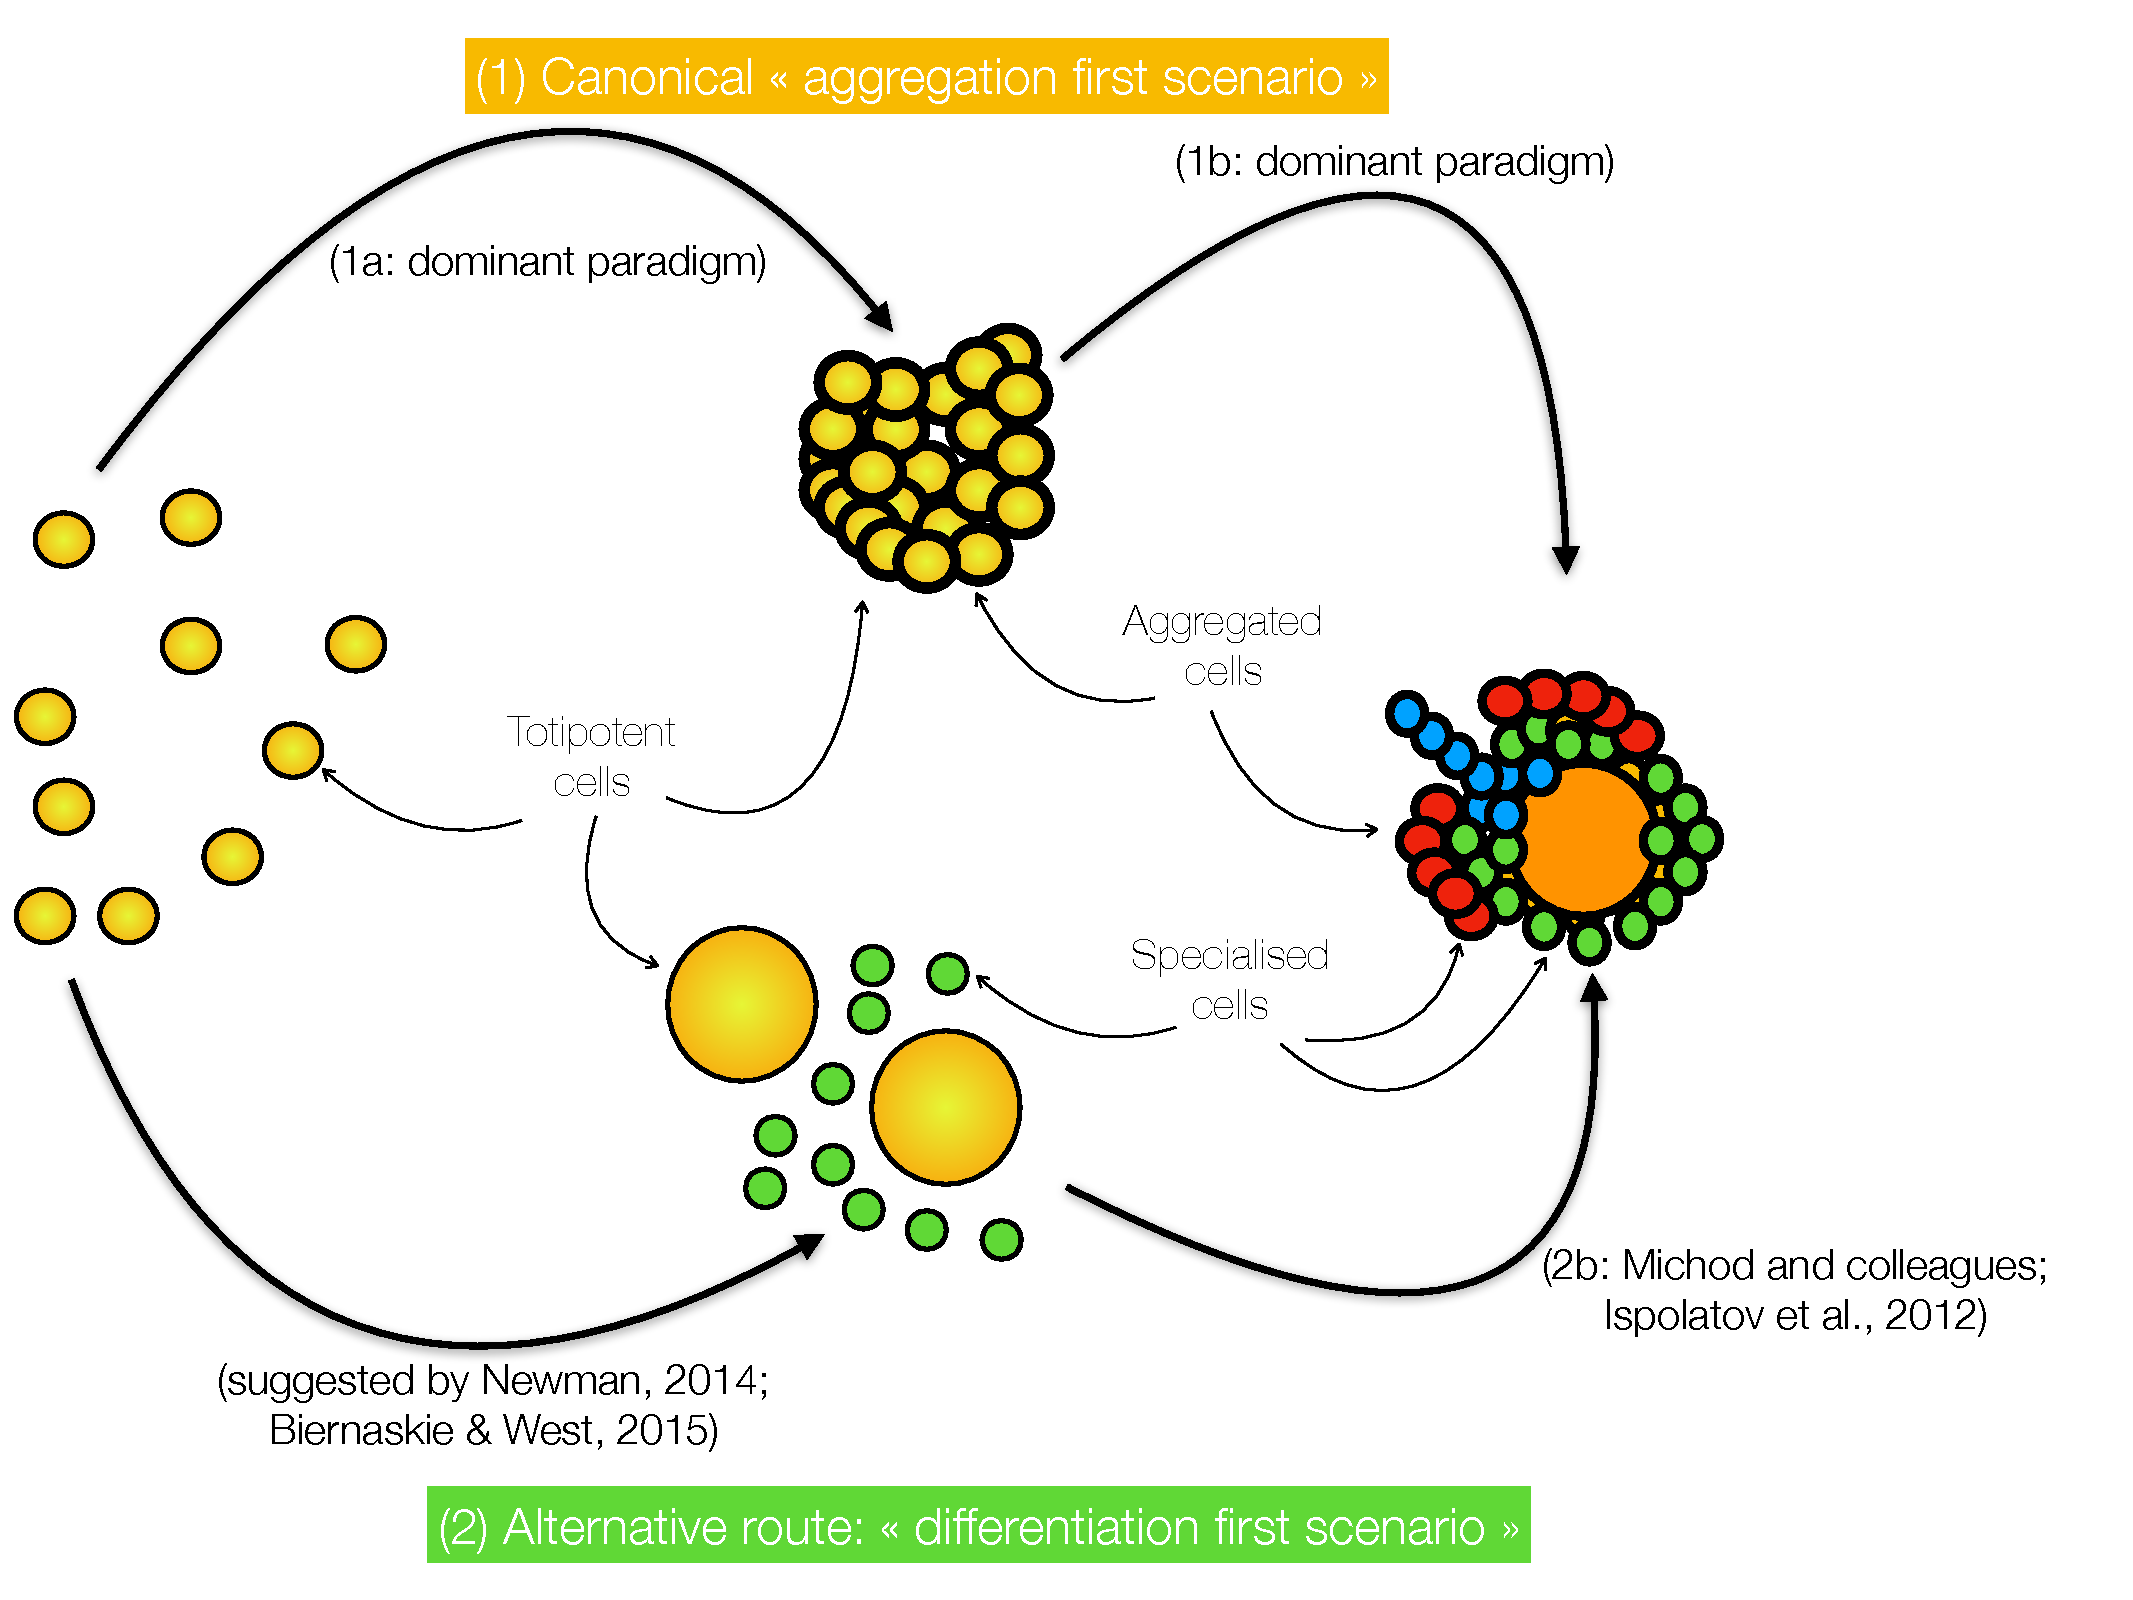
\includegraphics[scale=0.425,trim=0cm 0cm 1cm 0cm,clip]{pics/Cell-Diversity/Schema_route_to_multi.pdf}
    \caption{In the widely accepted "aggregation first scenario", differentiation occurs in already existing aggregates. Recently, \citet{Ispolatov12} have shown that multicellularity could evolve through the cooption of a differentiation behaviour pre-existing in solitary cells. Short after, \citet{BiernaskieWest15} developed a model suggesting coevolution between aggregation and cooperation, triggered by the emergence of aggregation. Meanwhile, \citet{Rokas08}, \citet{Ruiz-Trillo08} and \citet{Tikhonenkov20} have enlightened us about the ubiquitous presence of multicellular toolkit genes among unicellulars \citep{Sebe-Pedros16,Sebe-Pedros17,Ferrer-Bonet17}, and \citet{Niklas14} reminded us that differentiation can be advantageous even for unicellular organisms, which may have therefore paved the way for complex multicellularity \citep{Brunet17}.}
    \label{fig:EvoRoutes-Multi}
    \vspace{-0.5cm}
\end{figure}

For it triggered a dramatic increase in complexity and thereby in diversity, Evolution towards Multicellularity is considered one of the few Major Evolutionary Transitions - METs thereafter - Life came through during its course on earth \citep{Szathmary95,Szathmary15}. More precisely, this is an Evolutionary Transition in Individuality \citep{Michod96,Michod97,West15} - ETI - since it comes with a shift of the level on which Natural Selection operates \citep{Buss87}. During this transition, a transfer of fitness occurs that brings together lower level units into a collective to eventually form a higher level unit \citep{Okasha05,Bourrat15}. We review what makes these transitions special and how they foster Life diversity in section \textcolor{red}{compléter}. Hitherto, insights on ETIs have mostly stemmed from frameworks that rely on arbitrary - and \textit{ad hoc} - fitness functions, aiming to show under which conditions Natural Selection should promote division of labour among lower-level units, and, in turn, drive this transfer of fitness. More specifically, these functions involve two components -- fecundity and survival -- which are supposed to be subject to a trade-off whose convexity determines the benefit conferred by the division of labour \citep{Michod97,Michod05,Rueffler12,Nedelcu12}. Despite being rather artificial, this framework stimulated thoughts and provided the community with qualitative predictions where an explicit trade-off prevails and can readily be captured.

The great philosopher, Bertrand Russell, once said that \textit{the greatest challenge to any thinker is stating the problem in a way that will allow a solution}, and it is very true and even unavoidable. Of course, often in the History of Science, scientists have invented tools to answer their questions. Isaac Newton developed its methods of fluxions\footnote{Fluxion is Newton's equivalent for the (mathematical) differentiation notation concomitantly developed by Leibniz and which went down in history.} to understand the laws of motions \citep{Kleiner01} while Fisher imagined the analysis of variance at the onset of his career when he was starting to study population genetics \citep{Fisher19,Fisher21,Conniffe91}. But no matter how inventive scientists are, the invention still makes them look at their problem through a particular inflexible lens, as it were. In other words, stating the problem in a way that allows a solution impacts not only the solutions we find but also how we interpret these solutions. Thus far, the approach used by scientists interested in ETIs are faced with three closely related limitations. First, it focuses on the effect of an uncharacterized (and unrealistic) preexisting trade-off whereas identifying how it emerges from cellular underpinnings and its ensuing shape remains a conundrum. Meanwhile, how much the chosen definition for fitness - at both levels of individuality - can capture biological reality is anything but clear, to say the least, especially when division of labour facilitates the emergence of and/or exploitation of a new ecological niche. As a corollary, it is hard if not impossible to make quantitative - or even testable - predictions beyond simplistic experiments \citep{Ratcliff12,Bernardes21}. No less importantly, ignoring the mechanisms at the root of the trade-off(s) rules out the possibility for organisms to overcome them through other processes than the transition itself.  Finally, without specifying a genotype-phenotype map - explictly or implicitly - it is impossible to determine the genetic and ecological factors making this transition susceptible to happen (or preventing it). Our original goal was to tackle these issues by adopting a complementary approach based on a mechanistic framework.\\
%Multicellular organisms 

\textit{Yes, fitness is the central concept of evolutionary biology, but it is an elusive concept. Almost everyone who looks at it seriously comes out in a different place.}

Leigh Van Valen\\

Paradoxically, most foundational concepts in Science have proven to be contentious, fleeting and evanescent glimpses teetering as soon as one attempts to get close, akin speed and position which refuse to be captured together at the tiniest scales, questioning their very existence. Sometimes absolute as in Newton's Principia \citep{Greene99,Greene04}, sometimes relative as under Ernst Mach's pen \citep{Greene99,Raine75}, Space and Time have been tossed back and forth ever since They exist, and their ongoing turbulent journey is not finished at all now that they are woven in the same fabric \citep{Einstein05}, for their dimensionality is henceforth standing on the operating table of scientists \citep{Kaluza21,Klein91,Greene04}, awaiting to \textit{explain reality by the impossible} as pointed out by Alexandre Koyré \citep{Koyre73}. No one exactly knows, either, what Money is, other than a belief, nor is the role it plays on economic processes clear: while some proposed that it is purely neutral, especially in the long-run \citep{Friedman95,Hall18,Salerno20}, others thought that burying money to stimulate the creation of industries specialized at unearthing money would be better under certain circumstances such as a job crisis \citep{Keynes36}. Life also had its share of troubles going through the mind of scientists \citep{Schrodinger44,Forterre10,Weber10,,Tessera11}, as more than a hundred propositions have been recorded \citep{Trifonov11}, some of them would now willingly abandon completely the very idea of a definition to rely instead on a fuzzy logic \citep{Bruylants10} more capable to accommodate with a continuous scale from non-life to life and where, following Joseph Felsenstein, \textit{``Rocks [would be] the outgroup''} \citep{Felsenstein03}; but, as coal and oil may not be, one may question : "Which rock is the outgrup, Joe?"

Fitness has definitely earned its place in this distinguished family, and not only because Van Valen is always right. For a long while, Karl Popper denied to Evolution its scientific status on the ground that fitness is a tautology \citep{Popper76}, which it is, as long as one thinks that it is essentially a metrics\footnote{the same argument could be made for time}, as shown by the most basic theorems of Natural Selection \citep{Fisher30,Price72b,Wagner10,Queller17}. Fitness measures the ability of an entity to multiply (not to survive, contrary to a common shortcut) and as such can be the object of a measurement theory \citep{Wagner10} : in a sense, it is the idea that the more one reproduces in a lifetime, the more one will be represented as time goes by, an idea that Popper himself applied to highlight the evolutionary logic behind the scientific approach \citep{Popper72}. If each star -- or cloud, or whatever object one may think to -- gives birth to more stars after it has died, one will see a universe filled with more and more stars: stars would have a high fitness. Recently, the case has incidentally been made that there could be Natural Selection at the level of universes \citep{Smolin97}. At this stage though, it remains effectively untestable. The problem raised by Popper was that fitness measures the ability of an entity to survive but that we determined this ability by measuring the survival, giving rise to a circular reasoning. What makes Evolution a scientific theory is that fitness emerges from mechanistic underpinnings, a case which was recently made by \citet{Doebeli17}, albeit without getting past the metrics problem:  since they only insist on the importance of drawing fitness from birth and death contributions, they do not propose solutions to what fitness is in the first place.

Fitness is the ability of an organism to exploit its environment in order to multiply. Be it to apprehend quantitatively fitness transfers or even the mere effect of Evolution on cell phenotypes, we need to develop an approach where the mapping of phenotypes to fitness genuinely reflects cellular processes and their eventual trade-offs. Cell phenotypes result from the selective expression of proteins through regulatory networks, synchronized production of biomass through intertwined metabolic pathways comprised of enzymes. There have been previous woks where gene network governs the (Hogeweg, Beslon).

In a first work, we built such an evolutionary model where fitness arises from mechanistic underpinnings about genetic, cellular and metabolic processes. This framework is described in the first subsection of results. Using simulations, we demonstrated that  promote the evolution phenotypic heterogenity through , and how this degree of cellular individuality is canalized by the environmental stochasticity. Nevertheless, not knowing the shape of the genotype-phenotype-fitness map keeps from resolving which factors 

It turns out that building such multidimensional metabolic fitness landscapes from a theoretical point of view had not been achieved before. Because some of these dimensions can influence fitness and hence buffer each other weaknesses, they can partly explain why enzyme efficiencies resemble a zoo when gathered together \citep{Bar-Even11}. Along with genetic drift, this dimensionality had long been suggested as a possible explanation for this broad variability \citep{Hartl85,Clark91}. However, we have shown in Subsection \ref{Enzyme-Evolution} (article published in \textit{Molecular Biology and Evolution}) that this explanation is unlikely if not unfounded. Enzyme efficiencies should on the contrary be highly predictable when the mutation-selection-drift has established, while data indicate that they are in fact far more contingent on chemical and metabolic features than related to effective population sizes of organisms. Instead, we have shown that the existence of local metabolic constraints modulate fitness landscapes on which enzymes evolve. These key drivers are extensively studied in Subsection \ref{Enzyme-Evolution}.

Not only are enzyme efficiencies widely distributed, most of them are only moderately efficient and, even more surprisingly, far off their expected physical limits \citep{Bar-Even11,Bar-Even15}. Hence, enzyme efficiencies can be profoundly affected when the cellular content reaches a level that hinders the diffusion of macromolecules (short refs). 

Meanwhile, these moderate enzyme efficiencies significantly depart from the expected population genetics steady-state. As often in biology, this may result from numerous factors, such as the trade-off between protein activity and stability for instance. However, as discussed in the introduction of section (\textcolor{red}{XX}), this latter is unlikely to explain a pattern widely shared among enzymes, as it has been shown to be very enzyme and ecological conditions dependent. Yet, this mutationl load is not entirely unforeseen by theory. In the twilight of the XX$^{eth}$ century, \citet{Hartl96} and \citet{Poon00} have shown that complexity may come at a great cost. 

We discussed 

For quite a while, Science has relied on 
Biology is the science of interactions (citation Smolin)


\chapter{Evolutionary Principia of Cell Diversification}
\chaptermark{State of the art}

%\section{The ubiquity and protean nature of cell diversity}

%\subsection{Introduction: boundless diversity as the ultimate outcome of Evolution}

%\subsection{About cell diversification: }

%- Intro about spatial and temporal diversity (to say that cell diversification is different than cell diversity and focus on diversification occurring as a consequence of environmental pressures)
%Cell
%- Speciation and polymorphism
%- 
%- Multicellular differentiation

%\subsection{Cell diversification through the evolutionary looking-glass: rethinking the dichotomy between unicellular and multicellular organisms}

%Introduction on artificial classification (from a philosophical perspective)

%\section{The causes of Diversification: a tale of drift and trade-offs}

%\subsection{Drifting away from one another: Evolution without Adaptation sustains the Tree of Diversity}

%\subsection{Trade-off as the pervasive theoretical explanation for adaptive cell diversification}

%Aparté(A note on the construction of niche.)

%\subsection{Trade-off in Evolutionary Theory: shape and }

%\section{Cellular constraints as inescapable by-products of cell functioning}

%\subsection{Cell fitness as the product of metabolic pathways}

%About Michaelis Menten equations

%\subsection{Molecular crowding gives rise to an inescapable and universal cellular trade-off}

%\section{Gene networks: constraints, opportunities and in between}

%\subsection{Gene networks determines the rate and accessibility of phenotypes}

%\subsection{Gene networks can be exploited to produce a wide range of cellular behaviours} 

%\section{About modelling approaches in Evolution}

\chapter[Results]{Results}
\chaptermark{Results}
%\input{chapters/methods}

%\section{Insights on the evolution of cell phenotypic strategies from an explanatory model: use and misuse of mechanistic approaches in Evolution}

%\subsection{An evolutionary approach based on the intertwining of mechanistic processes}

%\subsection{\textit{In silico} Evolution favors phenotypic heterogeneity among generalist }

%\subsection{In search for the lost causality: the challenging issue of unravelling the drivers behind evolutionary outcomes in such models}

\section{A new perspective on enzyme evolution: finding a way towards predictability}\label{Enzyme-Evolution}

\subsection{Resource uptake and the evolution of moderately efficient enzyme}

This chapter was published in \textit{Molecular Biology and Evolution} (\url{https://doi.org/10.1093/molbev/msab132} ).

\subsubsection{Abstract}

Enzymes speed up reactions that would otherwise be too slow to sustain the metabolism of self-replicators. 
Yet, most enzymes seem only moderately efficient, exhibiting kinetic parameters orders of magnitude lower than their expected physically achievable maxima and spanning over surprisingly large ranges of values. Here, we question how these parameters evolve using a mechanistic model where enzyme efficiency is a key component of individual competition for resources. We show that kinetic parameters are under strong directional selection only up to a point, above which enzymes appear to evolve under near-neutrality, thereby confirming the qualitative observation of other modelling approaches. 
While the existence of a large fitness plateau could potentially explain the extensive variation in enzyme features reported, we show using a population genetics model that such a widespread distribution is an unlikely outcome of evolution on a common landscape, as mutation-selection-drift balance occupy a narrow area even when very moderate biases towards lower efficiency are considered. Instead, differences in the evolutionary context encountered by each enzyme should be involved, such that each evolves on an individual, unique landscape. Our results point to drift and effective population size playing an important role, along with the kinetics of nutrient transporters, the tolerance to high concentrations of intermediate metabolites, and the reversibility of reactions. Enzyme concentration also shapes selection on kinetic parameters, but we show that the joint evolution of concentration and efficiency does not yield extensive variance in evolutionary outcomes when documented costs to protein expression are applied.

%\keyword{Enzyme evolution, Enzyme kinetics, $k_\text{cat}/K_M$, $k_\text{cat}$, Facilitated diffusion, Michaelis-Menten}

%\maketitle

\subsubsection{{Introduction}\label{sec:Intro}}


Living organisms need to uptake and metabolize nutrients, relying on enzymes to catalyse chemical reactions along metabolic pathways. Accordingly, and despite being intrinsically reversible \citep{Haldane30,Klipp94}, \textit{in vivo} enzyme-catalyzed reactions are commonly thought of as an irreversible two-step process \citep{MichaelisMenten1913,Bar-Even11,Bar-Even15,Johnson11}:
\begin{equation}
\ce{ E + S <=>[k_{f}][k_{r}] ES ->[k_{cat}] E + P },
\label{chemMM}
\end{equation}
where $k_f$ and $k_r$ are the rates of association and dissociation between enzyme and substrate, and $k_\text{cat}$ is the turnover number, that is the rate of formation of the product $P$ from $ES$ complexes. The first part of this chemical equation describes the encounters between the enzyme $E$ and the substrate $S$; the enzyme will be efficient if $ES$ complexes form often and do not dissociate before the substrate has been turned into a product, which is reflected by the constant $K_\text{M}=\dfrac{k_\text{r}+k_\text{cat}}{k_\text{f}}$. The efficiency $v$ of an enzyme -- the rate at which it makes a product $P$ from $S$ -- depends on these two constants through equation (\ref{EquiBHsimp}):
\begin{equation}
v=k_{cat}.[E_\text{tot}].\frac{[S]}{K_\text{M}+[S]},
\label{EquiBHsimp}
\end{equation}
\noindent under the assumption that the concentration $[S]$ is approximately constant and that of $[ES]$ is at steady-state \citep{MichaelisMenten1913, Briggs25}.
 
At first glance, Natural Selection is presumed to optimize enzymatic efficiency by pushing $k_\text{cat}$ upwards and $K_\text{M}$ downwards to universal physical limits. Enzyme efficiencies are for instance limited by the diffusion properties of their aqueous environment, which sets an upper bound of approximately $10^8-10^{10} M^{-1}s^{-1}$ for the ratio ${k_\text{cat}}/{K_\text{M}}$  \citep{Alberty58,Zhou82}. Nearly optimal enzymes indeed seem to exist, as exemplified by triosephosphate isomerase (TIM) whose ratio is close to this theoretical ceiling \citep{Knowles77}. But they are uncommon: most enzymes appear to be only moderately efficient and far off these physical limits -- including enzymes immediately flanking TIM in the glycolysis metabolic pathway \citep{Davidi18}.
Indeed, \citet{Bar-Even11} have analysed a dataset of several hundreds of enzymes and found a wide diversity among enzyme parameters, thus sketching a puzzling pattern that has far more in common with a zoo than it looks like variations around an archetypal form.\\

%To date, three sources of explanations have been invoked to explain both the reported variance in parameter estimates and the fact that many look suboptimal: (1) \textit{in vitro} estimates do not reflect the \textit{in vivo} functioning of enzymes, (2) physical constraints vary between enzymes such that their achievable optima differ, and (3) Evolution fails to produce optimum properties.\\

This wide distribution of enzyme features could partly be explained by differences between enzyme behaviour \textit{in vivo} and \textit{in vitro}. Such differences are expected, first because diffusion in a test tube is hardly comparable to diffusion in the cytoplasm \citep{Ellis01,Rivas04,Zhou08,Rivas18}. As the cytoplasm gets packed, the cell approaches a state where molecules are less mobile, hindering substrate-enzyme encounters \citep{Muramatsu88,Zimmerman93,Blanco18}. In this regard, $K_\text{M}$ values are likely underestimated \textit{in vitro}, and enzymes should perform less efficiently \textit{in vivo}. Simultaneously, macromolecular crowding can sometimes improve catalytic activity \textit{in vivo}, making specificity constants $k_\text{cat}/K_\text{M}$ higher than their \textit{in vitro} estimates \citep{Ralston90,Ellis01,Jiang07,Pozdnyakova10}. Crowding effects are obviously important for our understanding of enzyme evolution but, alone, they are definitely too weak to explain the wide variability across enzymes insofar as their reported estimates typically lie in the range of one order of magnitude \citep{Davidi16}. \\%In addition, the combination of these opposing effects should buffer the overall effect each one would separately have on activity as detailed above \citep{Tabaka14,Zhou08}.%J'ai l'impression qu'on pourrait se passer de cette dernière phrase, et expliquer au reviewer que c'est déjà présent finalement.

Another source of explanation to the observed distribution of enzymes (in)efficiencies is a failure of Evolution to consistently optimize them, possibly due to physical constraints. Indeed, \citet{Heckmann18} have shown how a variety of $k_\text{cat}$s may evolve provided that some of them are physically constrained. Besides the diffusion limit already mentioned, constraints on enzyme evolution might include an intrinsic trade-off \citep{Gudelj10,Stiffler15} that originates from the dependency of both $k_\text{cat}$ and $K_\text{M}$ on intermediate energy profiles \citep{Heinrich91}. Nonetheless, this trade-off is scarcely observable among evolved enzymes -- \citet{Bar-Even11} report a coefficient of determination around $0.09$ for the correlation between $\log_{10}(k_\text{cat})$ and $\log_{10}(K_\text{M})$ -- suggesting that it can be overcome. 
Other constraints may exist and be specific of a given reaction \citep{Klipp94} -- \textit{e.g.} reaction reversibility -- potentially explaining a part of the variance in enzyme efficiencies.
It remains that estimating constraints on all individual enzymes appears like a daunting task, which could be guided, in part, by the identification of deviations from evolutionary predictions.\\


Following this idea, the premise of our theoretical investigation into the origins of enzyme diversity is that it results mainly from unconstrained evolution, such that the reported differences may be caused by the combined action of selection and genetic drift. It is important to notice that the information we have is partial, as an enzyme's activity is the joint result of its kinetic constants and cellular concentration, perhaps also contributing to the reported variance in the former. In fact, \citet{Davidi16}'s method to determine \textit{in vivo} turn-over rates lends some credence to the idea that increased levels of expression make up for lower kinetic constants \citep{Davidi18}. 
%But protein extra expression comes at a great cost for fitness \citep{Wagner05,Lang09,ScottM10,Noor16,Kafri16}, as it requires both energy and matter \citep{Novick57,Stoebel08,Wagner05,Lynch15} and as the efficiency of physical processes may depend heavily on an optimal intermediate content \citep{Dong95,Dill11,Andrews20}. 
It is therefore obvious that an enzyme's expression needs to be considered as another dimension of its activity, especially since it has been shown that the evolutionary tuning of gene expression can happen very quickly \citep{Dekel05}.

Concomitantly, an enzyme's activity can be impacted by protein misfolding, which reduces the effective enzyme concentration \citep{Tokuriki09,Yue05,Drummond05,Echave17a} while also impacting fitness by enhancing protein erroneous interactions \citep{Yang12} and the formation of toxic protein aggregates \citep{Bucciantini02,Sabate10,Geiler-Samerotte11}. Protein stability is thus under strong purifying selection to avoid the deleterious effects of misfolding \citep{Drummond08}. Accordingly, it has been shown that proteins have evolved to stand beyond a stability threshold \citep{Bloom05}, although marginally \citep{Taverna02}. 
%Through the fact that mutations are on average destabilizing \citep{Tokuriki07,Tokuriki08}, there exists a well-known trade-off between stability and activity \citep{Shoichet95,DePristo05,Tokuriki08}. 
Because mutations are on average destabilizing, this definitely narrows down the spectrum of adaptive mutations \citep{Shoichet95,DePristo05, Weinreich06,Tokuriki07,Tokuriki08, Lunzer10}. Nevertheless, several studies have reported the existence of a genotype space where activity can be optimized without compromising stability \citep{Schreiber94,Burg02,Bloom04,Knies17,Miller17}. Even when improving function requires the fixation of destabilizing mutations, compensatory mutations can in principle cancel out stability losses arising from active site evolution \citep{DePristo05,Tokuriki08,Tokuriki09,Storz18}. Adaptive evolution may even be facilitated by preexisting mutational robustness against misfolding \citep{Bloom06,Bloom07}. Therefore, although the requirement of a stable, correctly folding protein may sometimes slow down the evolutionary process, it is rather unlikely that stability explains the distribution of enzyme kinetic parameters albeit marginally.\\

%Together with the fact that \citet{Bar-Even11} shown a clear-cut influence of enzyme pathways

%Peut-être faudra-t-il un peu revoir cette structure, car je trouve finalement un peu bizarre de couper entre ces éléments explicatifs.


Enzyme kinetics evolution has often been considered theoretically through the lens of flux control \citep{Burns85,Clark91,Fell92,Kacser95,Yi19}. Indeed, the control of the flux in a metabolic pathway is shared between all enzymes, in what is known as the summation theorem \citep {Kacser73,Heinrich74}. Thence, because the sum of control coefficients must equal 1 within a pathway, if all enzymes have similar kinetic parameters, none of them exerts a strong influence \citep{Dean95}. But if one enzyme departs from this trend and becomes inefficient, it exerts a strong control at the expense of others \citep{Dykhuizen90}. This leads to diminishing-returns epistasis in which the fitness landscape flattens because, as an enzyme becomes more efficient, subsequent mutations have smaller effects \citep{Kacser73,Dykhuizen87,Tokuriki12}, a finding that has since received empirical confirmation \citep{Fell92,Dean95,Lunzer05,Yi19,Chou14}.

%Flux control theory have come to the conclusion that the activity of individual enzymes should evolve on fitness landscapes exhibiting diminishing returns epistasis, such that enzymes should quickly reach a fitness plateau.
 \citet{Hartl85} and \citet{Dean86} have considered such a fitness landscape under a population genetics framework to conclude that enzymes may quickly reach a fitness plateau and evolve on nearly neutral landscapes \citep{Ohta92}. Nonetheless, these studies fall short of explaining why inefficient enzymes having stronger control do not evolve higher activities \citep{Yi19}. In these models as in most, an enzyme's efficiency is captured by its activity, generally represented by a composite of $k_\text{cat}$, $K_\text{M}$ and enzyme concentration \citep{Hartl85,Clark91,Chou14,Kaltenbach14}, such that the distinct evolutionary dynamics of these parameters, together with an enzyme's concentration, is ignored. This reduction of an enzyme's dimensionality goes against the empirical observation that each dimension may have a differential impact on fitness in the context of antibiotic resistance \citep{Walkiewicz12,Stiffler15,Rodrigues16} and that each is thus necessary to predict evolutionary outcomes \citep{Walkiewicz12}.\\

Perhaps more importantly, \citet{Heinrich91} and \citet{Schuster08} have pointed out that these modelling frameworks assume a constant value for either or both concentrations of the first substrate and of the final product \citep{Orth10}, whereas Evolution should instead maximize the amount of final products generated. \citet{Klipp94} found that the aforementioned concentrations indeed have a major influence on optimal rate constants under certain assumptions. 
Likewise, nutrient uptake is most often not considered explicitly in existing models of enzyme evolution, while it is obviously critical in the competition for resources \citep{Dykhuizen94}. 

Nutrient uptake occurs when metabolites move inwards across cell membranes; it may rely on membrane permeability only (passive diffusion) or involve channels and carrier proteins, be they transporters or cotransporters \citep{Stein86a}.
Here we build a model that explicitly includes passive (PD hereafter) or facilitated diffusion (FD) followed by an unbranched metabolic pathway to study how resource availability coupled to transport modulates the evolution of enzymes along the pathway.
In ecological scenarios where individuals compete for resources, Natural Selection should favour genotypes that maximize the net intake of molecules and their transformation, which are linked under both PD and FD.

Based on this premise, we confirm that the evolution of enzyme kinetic parameters $k_f$ and $k_\text{cat}$ takes place on cliff-like fitness landscapes where a fitness plateau covers a wide part of the relevant parameter space. Kinetic parameters have co-dependent but distinct evolutionary dynamics -- and thus distinct sensitivities to certain parameters of the model -- such that the shape of the plateau can be modulated by changing parameters of the model within realistic ranges. We show that this fitness landscape depends on features of transporters that initiate a metabolic pathway, along with parameters that vary among enzymes within a pathway, like the tolerance to high concentrations of intermediate metabolites or the reversibility of reactions.

We further demonstrate, using a simple population genetics model, that the evolutionarily expected features of an enzyme should be predictable, even though enzymes evolve near-neutrally on the fitness plateau. This is because the model includes slightly biased mutations that tend to produce a majority of less efficient enzymes. We thus postulate that the wide variety of enzyme features reported might be explained in a large part by differences in the shape of their fitness landscapes. While testing this hypothesis will require extensive information about individual enzymes, we made a small step in this direction, showing that enzymes involved in metabolic pathways with different types of transporters exhibit differences that our model qualitatively predicts.  

\subsubsection{Results\label{sec:Results}}

\paragraph{\noindent Passive diffusion is generally inadequate to sustain cell metabolism}

In the version of our model in which intake relies on passive diffusion (PD), the net uptake of a nutrient is a direct outcome of its concentration gradient, and therefore of how efficiently the first enzyme catalyses its transformation inside the cell. Assuming that fitness is proportional to the flux of product of this reaction, we find that the fitness landscape has a cliff-like shape with fitness increasing steeply as parameters $k_\text{cat}$ and $k_f$ increase (see Supplementary materials, section Text S1). The precise shape will not be commented in detail here, for it is very similar to landscapes obtained under facilitated diffusion (FD, treated in the rest of this manuscript). 

Importantly, our results indicate that PD can only sustain a small part of the metabolism of most living cells given cell permeabilities reported in the literature \citep{Wood68,Milo10}, suggesting that this process may not be a determining factor in the evolution of enzymes along metabolic pathways. Indeed, even extremely efficient enzymes, harbouring values of $k_\text{cat}$ and $k_\text{cat}/K_\text{M}$ close to their physical limits, yield low inward fluxes that approach $10^{-2}~mM.s^{-1}$ when considering a spherical cell with a diameter $D=1 \mu m$. To get a sense of how low these fluxes are, we calculated the maximum cell size they can theoretically sustain. Considering that basal metabolic demands are approximately proportional to the cell volume and using estimates by \citet{Lynch15} for this relationship, we predicted the maximum size enabled by sugar passive diffusion (see \ref{sec:M&M} - Materials and Methods). Setting a (conservatively high) medium concentration in glucose $[G]=1$M yields a theoretical volume ceiling $V_{est}=0.84 \mu m^3$. 

Nearly all eukaryotes, and most prokaryotes are \textit{de facto} larger than this threshold \citep{Heim17}, which might help explain the apparent ubiquity of FD. While this demonstration hinges on numbers for sugar uptake, which may arguably be the task requiring the highest flux, PD may be limiting for many other metabolites \citep{Boer10}, depending on their permeability and availability in the environment: even for very high amino-acids concentrations that may only be met in multicellular organisms \citep{Schmidt16} and assuming the highest observed permeability for such metabolites \citep{Chakrabarti94}, these levels are orders of magnitude lower than with FD (see Supplementary material - section Text S1 for PD results).

\noindent \paragraph{General shape of the fitness landscape under facilitated diffusion}

For most metabolites, FD relies on the specific binding of the substrate to transmembrane carrier proteins (transporters hereafter), followed by its translocation to the other side of the membrane \citep{danielli1954,Kotyk67,Stein86d}. Our model builds on \citet{Kuile94}'s approach to model FD, considering the simplifying assumption of symmetric transport. Within this framework, FD operates on the concentration gradient \citep{Bosdriesz18} and is susceptible to saturation, represented by constant $K_T$ -- similar to $K_M$ in the Michaelis-Menten equation -- and an interaction constant $\alpha$ (see Methods for details). We assessed how this saturation phenomenon influences the selection pressure acting on forward enzyme kinetic parameters ($k_f$ and $k_\text{cat}$) under various scenarios. 

\begin{figure*}[t!]
\centering
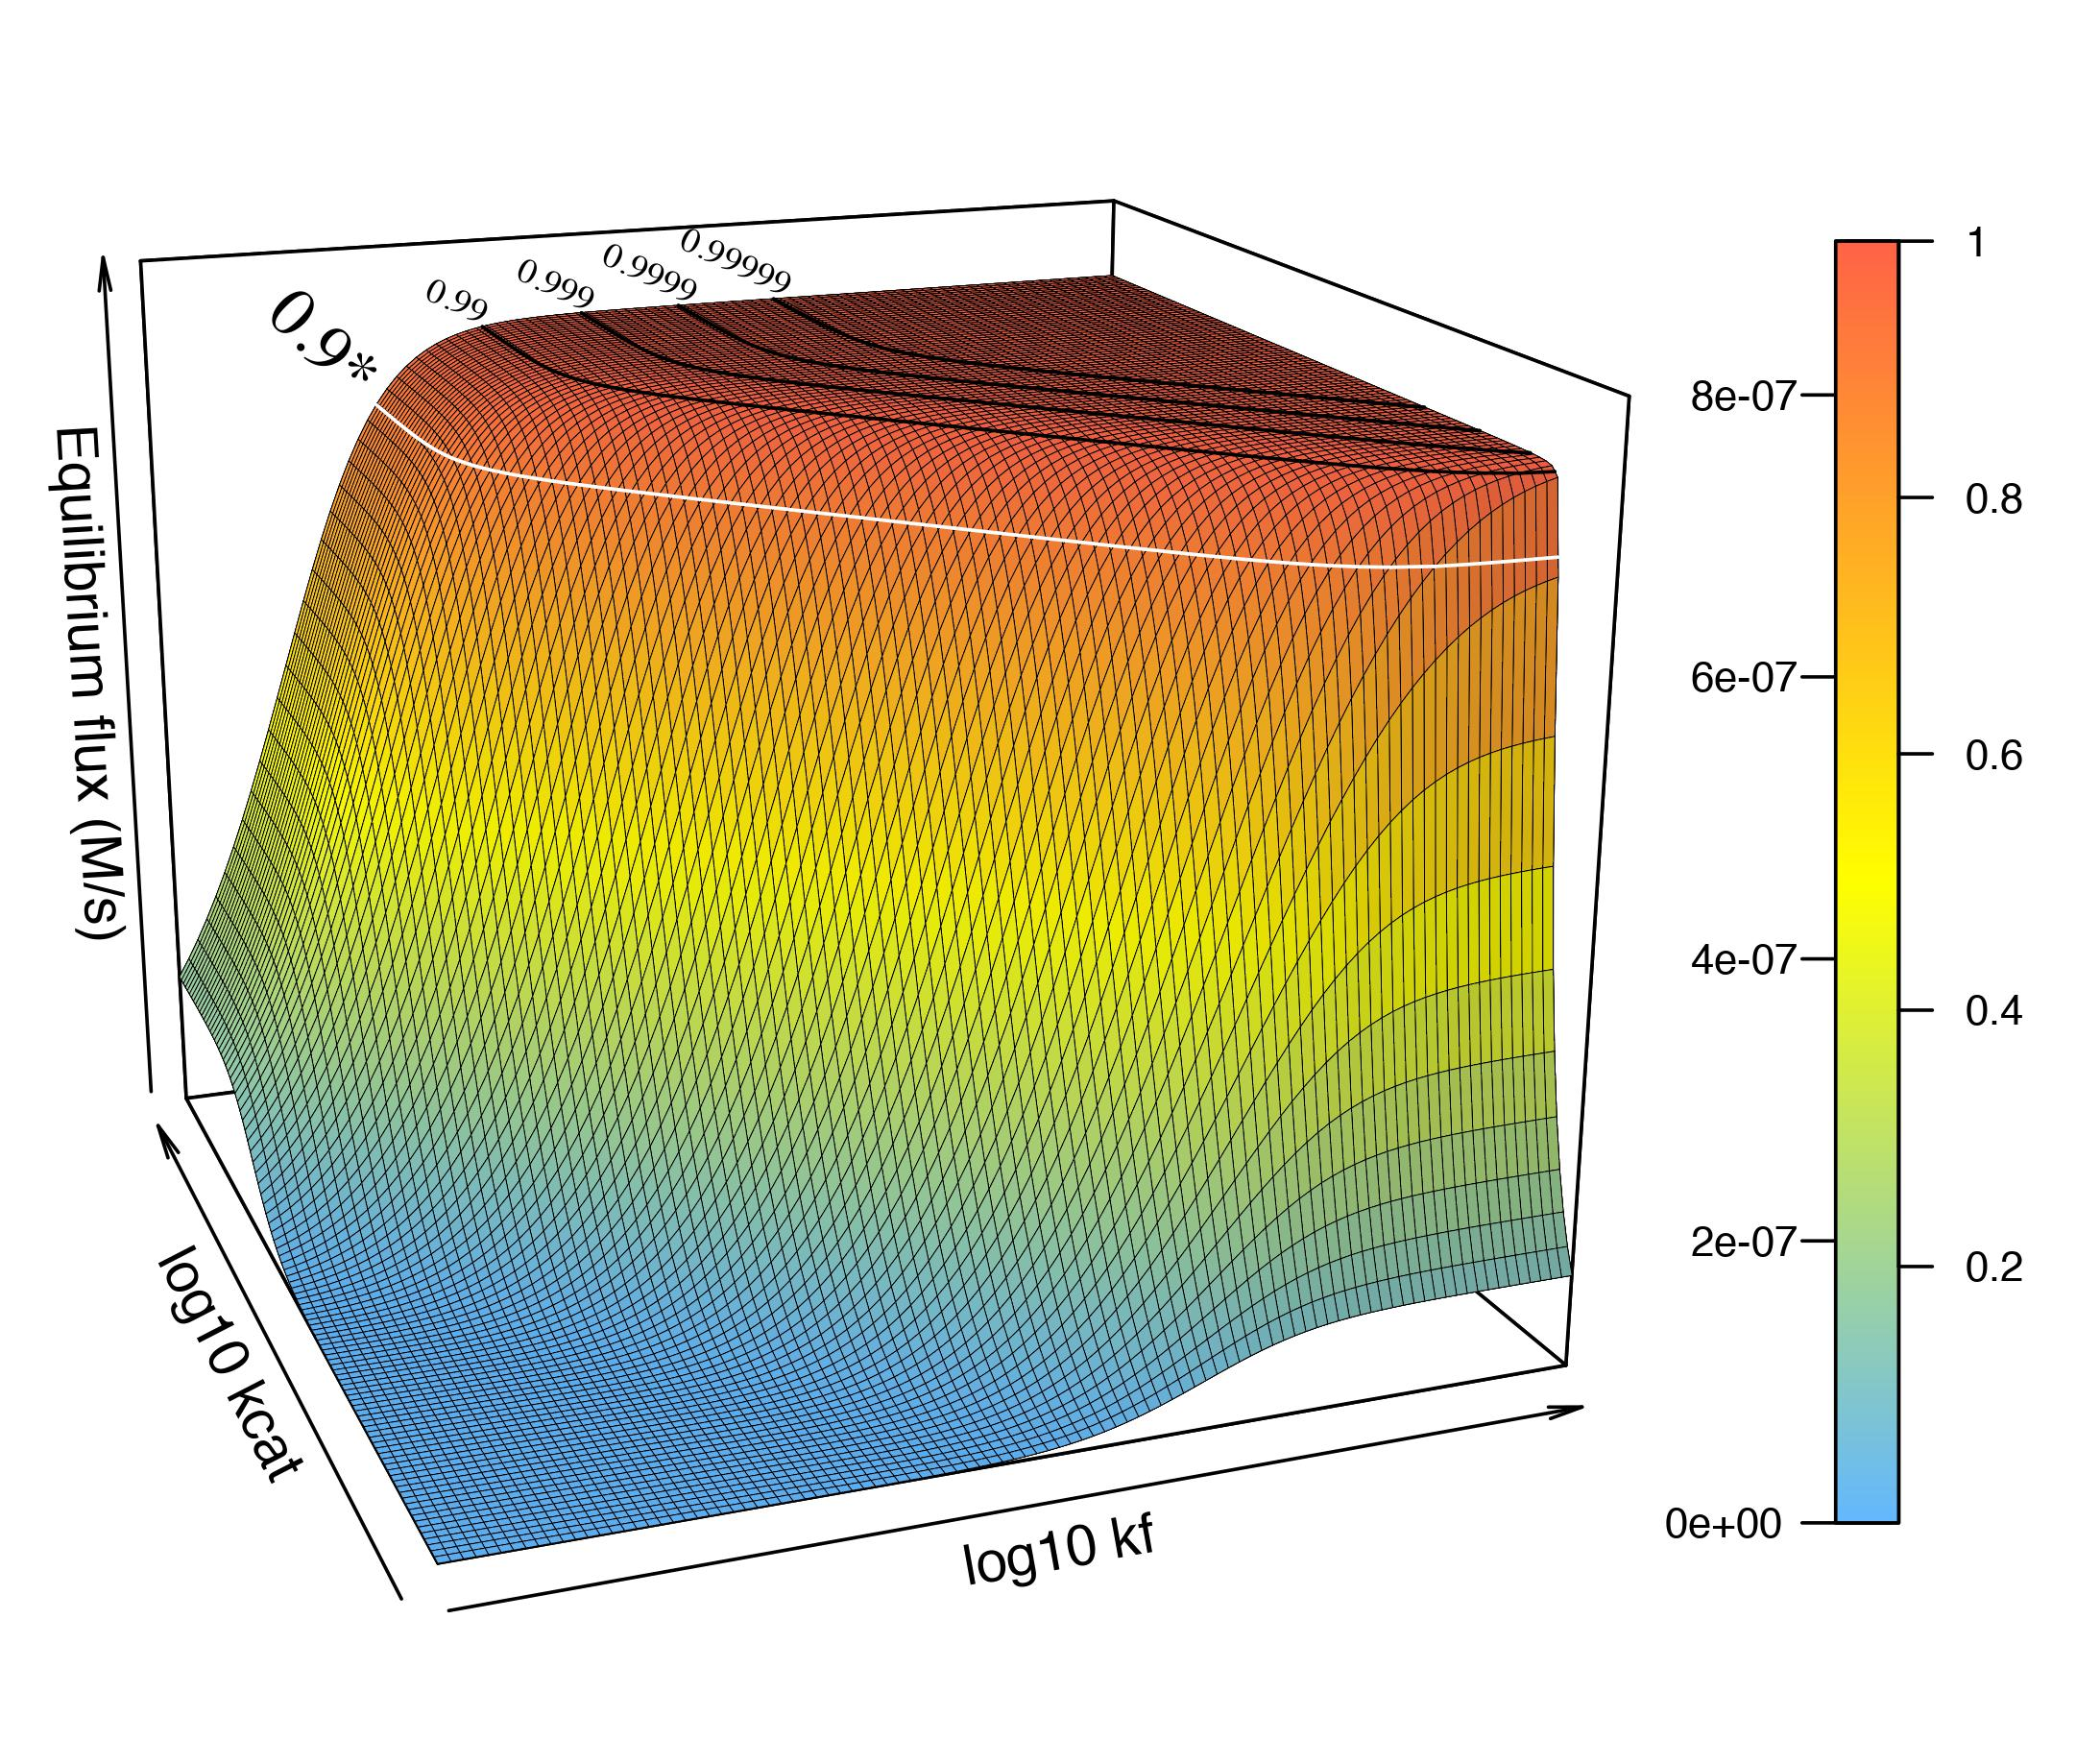
\includegraphics[scale=0.55,trim=0cm 0.5cm 0 1cm,clip]{pics/Enzymes/3DFitLandscape.jpeg} 
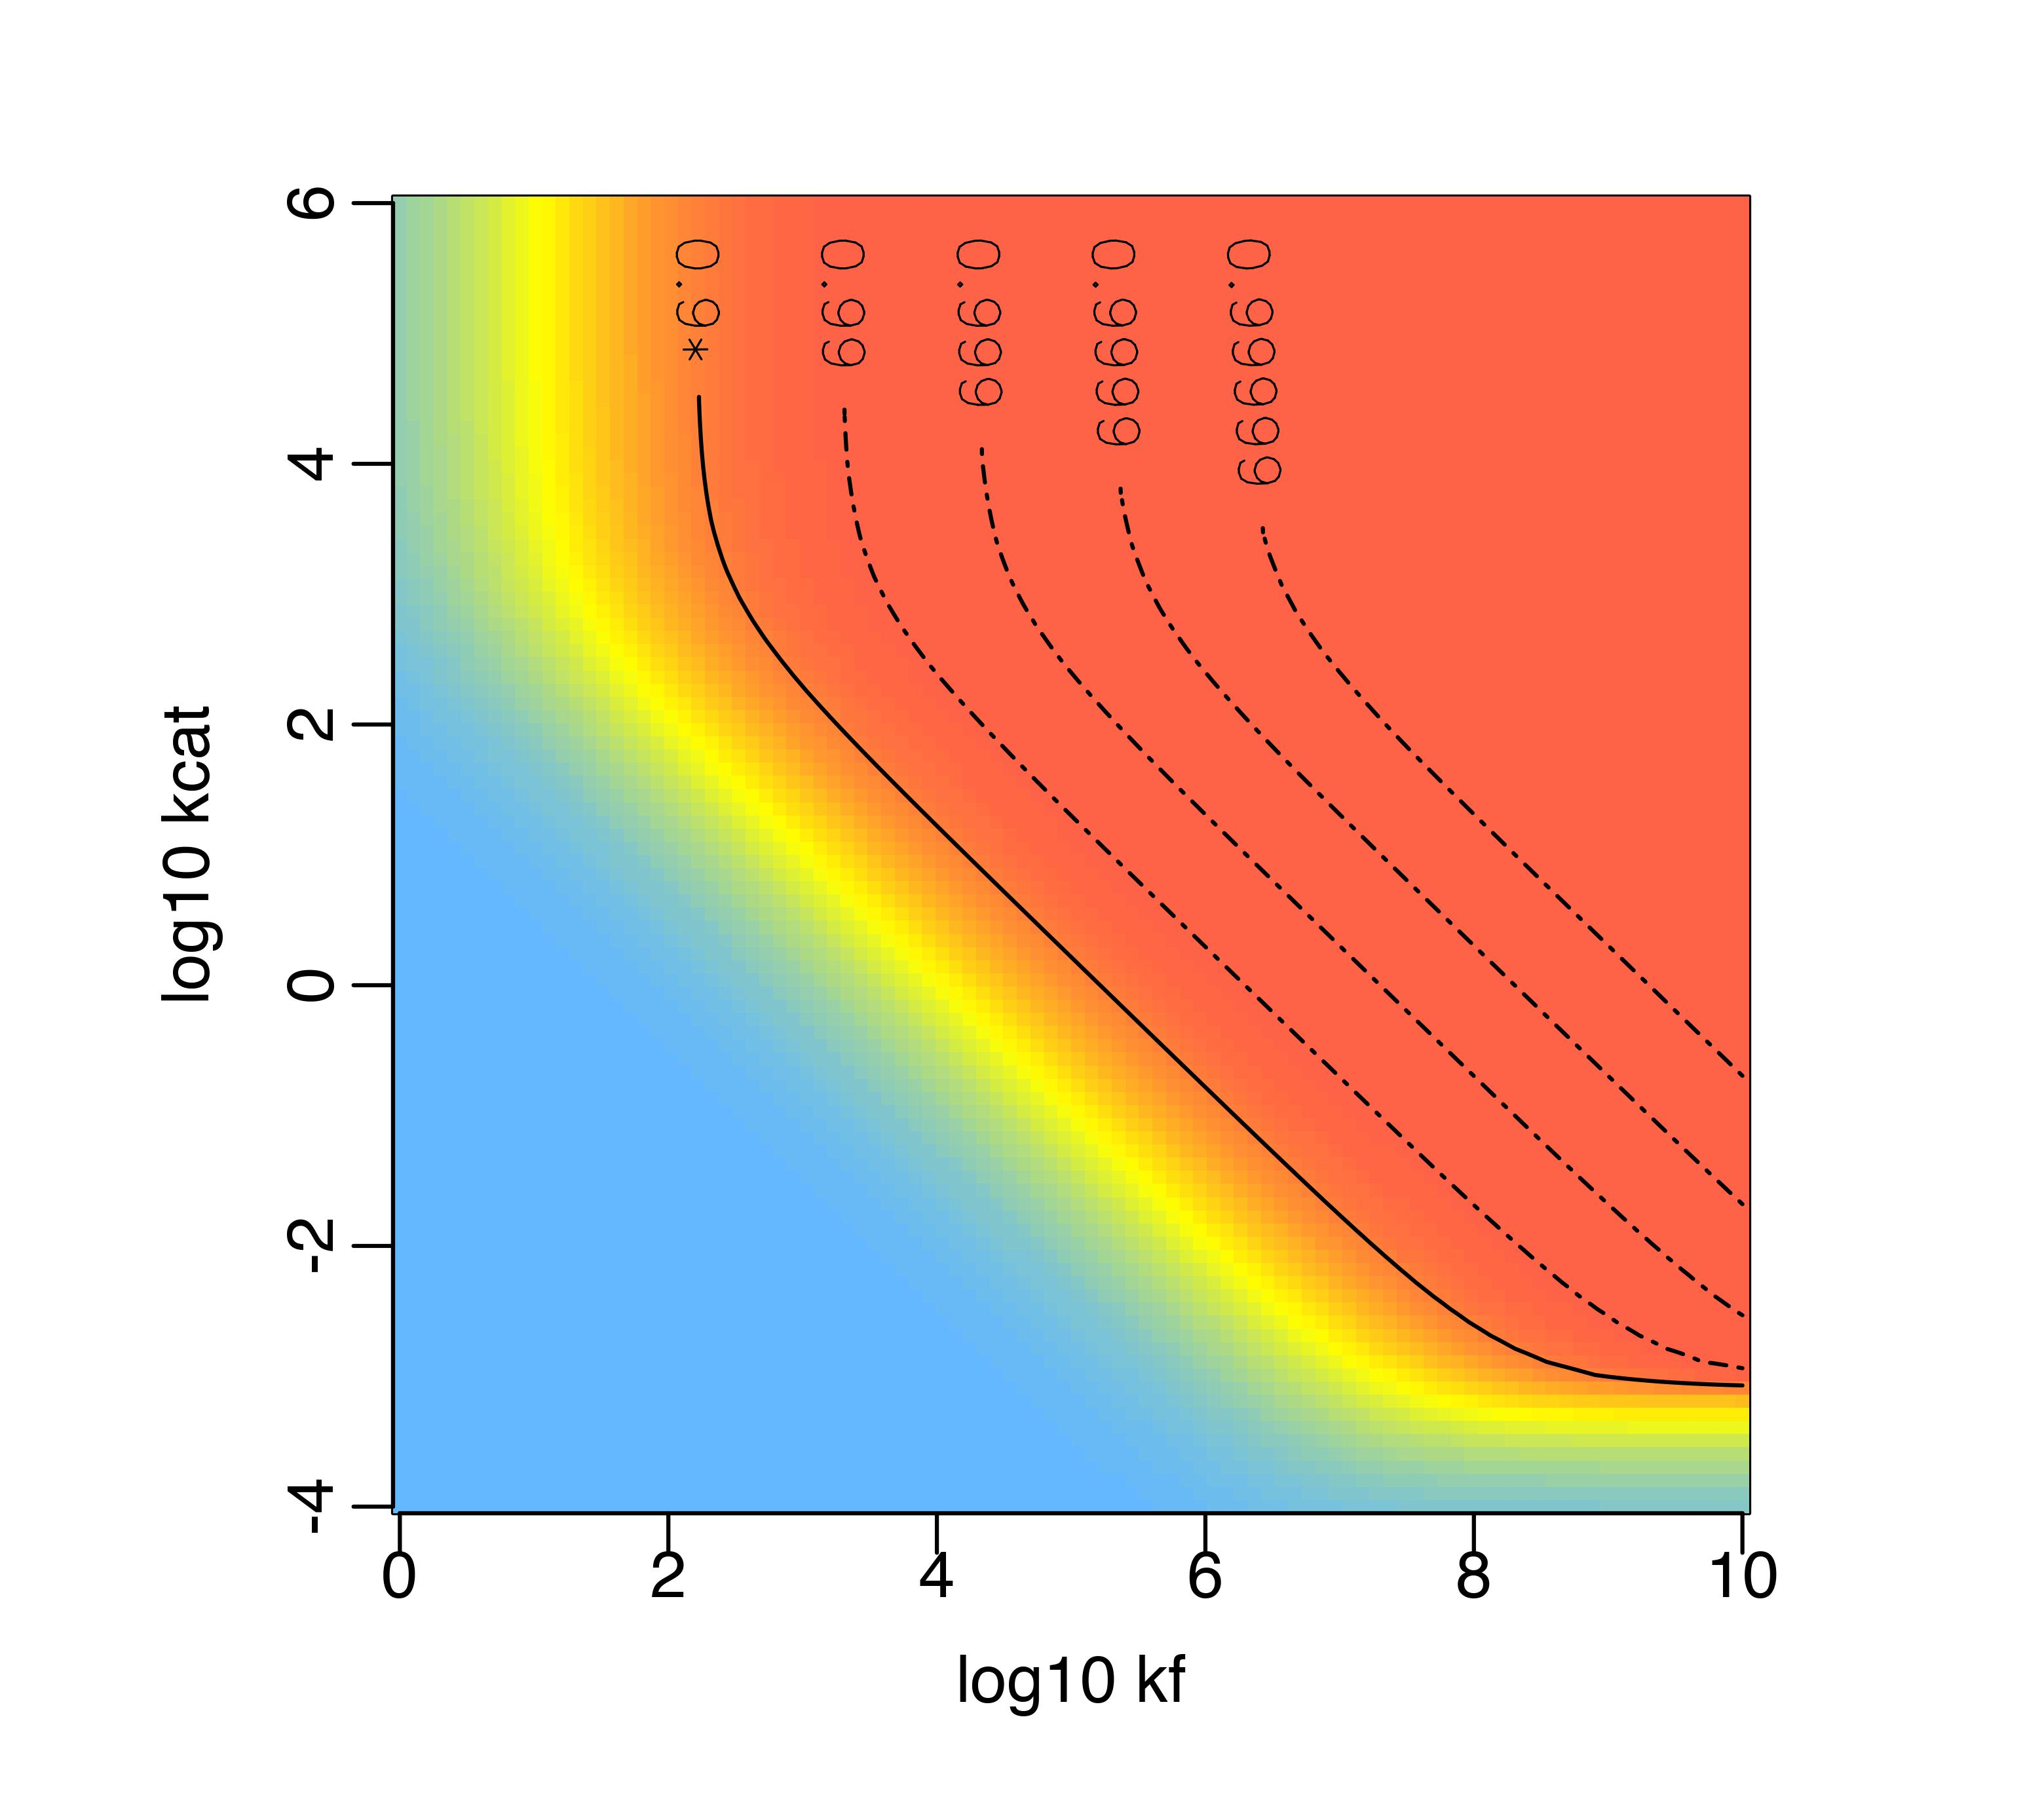
\includegraphics[scale=0.55,trim=0 0cm 0cm 0.5cm,clip]{pics/Enzymes/2DFitLandscape.jpeg}  
%\vspace{0.5cm}
\caption{The flux of product following substrate uptake by transporters and conversion by a dedicated enzyme depends on kinetic parameters $k_f$ and $k_\text{cat}$. This landscape is based on a moderately low flux at saturation $V_{Tm}=1 \mu M.s^{-1}$ close to those measured for amino acids and nucleosides in E.\textit{coli} \citep{Zampieri2019}. We also set the transport saturation ratio $[S_\text{out}]/K_\text{T}$ to 10 such that the FD process approaches saturation, and relatively high transporter affinity $K_\text{T}=50\mu M$, also in line with estimates for nucleosides \citep{Griffith96,Xie04}. Other parameter values include $k_r=10^3s^{-1}$ and $[E_{tot}]=1mM$. The color gradient indicates the absolute and normalized (with a maximum flux of $1$) values of equilibrium flux.
}
\label{figure3D2DFit}
\end{figure*}

In order to depict a fitness landscape representative of an average enzyme, we first consider a situation where transporters induce a moderately low rate $V_{Tm}$ and saturate with a relatively high affinity -- corresponding to a low $K_T$ (FIG.~\ref{figure3D2DFit}). In this situation, the inward flux at steady-state (which, as argued in the introduction, can be considered representative of fitness) forms a plateau when the upstream enzyme in the metabolic pathway has high $k_\text{cat}$ and $k_f$. This low equilibrium flux elasticity coincides with the saturation theory \citep{Wright34, Kacser73,Hartl85,Dykhuizen87,Dean95,Yi19}, especially with its version incorporating facilitated diffusion \citep{Kuile94,Dean95}. The flux plateau is delineated by parallel isoclines (solid and interrupted lines in FIG.~\ref{figure3D2DFit}) oriented in the bottom-right direction of the landscape for intermediate values of $k_\text{cat}$ and $k_f$, such that decreasing $k_f$ by one order of magnitude can be compensated by a similar increase in $k_\text{cat}$. While this mutual dependency holds even for high $k_f$ values as long as $k_\text{cat}$ is not critically low (\textit{i.e.} when $k_\text{cat}>10^{-3}$), it stops when $k_\text{cat}\geq 10^3$, where increasing $k_\text{cat}$ no longer improves fitness. 
%%% On ne peut pas faire le commentaire suivant en s'appuyant sur la fig 1
%This negative relationship in a part of the isocline depends on the dissociation rate of enzyme-substrate complexes, $k_r$. As $k_r$ decreases away from $k_{cat}$, the isocline progressively loses this oblique part (Fig.~\ref{figure3D2DFit}), a trend that will be fully appreciated below. 
Besides, the influence of $k_\text{cat}$ and $k_f$ is not strictly equivalent, since the increase in flux is more gradual in response to $k_f$. 
 
Furthermore, and contrary to the textbook picture whereby most biological reactions are not limited by diffusion at all \citep{Bar-Even11,Sweetlove18}, increasing an enzyme's association rate $k_f$ – be it through its diffusivity or its binding rate – may still enhance the equilibrium flux when diffusion is substantially faster than catalysis.

\noindent \paragraph{Properties of facilitated diffusion modulate the landscape}

To explore the effect of FD kinetics on the evolution of enzymes in the metabolic pathway, we studied the influence of  $K_T$ -- the affinity of the transporter for the substrate -- and $V_{Tm}$ -- the maximum transport rate -- still assuming that the substrate is close to saturation ($[S_\text{out}]/K_T=10$). We find that increasing the transport flux $V_{Tm}$ exerts a positive selection pressure on kinetic parameters for the upstream enzyme (\textit{i.e.} for increasing $k_\text{cat}$ and $k_f$). The plateau is shifted accordingly (see FIG.~\ref{figure2DSSatStud}-A), towards the top-right corner of the landscape, at a distance that corresponds to the magnitude of the change in $V_{Tm}$. Increasing the affinity of the transporter (\textit{i.e.} decreasing $K_T$), however, selects for higher $k_{f}$ (the isoclines are displaced to the right and the fold change is similar to that of $K_T$) but has no other visible influence on $k_\text{cat}$ than increasing its codependency with $k_f$, a result that holds regardless of the flux at saturation $V_{Tm}$ (notice that we only considered high $V_{Tm}$s, larger than in the average case, because these cases are more likely to be under directional selection). 

This specific effect on the affinity of the upstream enzyme is likely due to a competition between the transporter -- which can transport the substrate in both directions -- and the enzyme, which harvests the substrate at a rate that depends on the dissociation constant $K_D=k_r/k_f$. It should be noted that nutrients under lower demands -- \textit{e.g.} amino acids -- are generally less concentrated in the environment, often coinciding with a higher affinity of their transporter. Therefore, the possible combinations of flux and affinity likely occupy a restricted space of possibilities where flux and affinity are negatively linked \citep{Gudelj10,Bosdriesz18}, which as can be seen in SM Figs.~S3-A,E,I results in landscapes that mainly differ by the minimum value of $k_\text{cat}$ on the plateau. In FIG.~\ref{figure2DSSatStud}-A, we have considered ranges of empirical estimates for sugars (high flux with low to moderate affinity) \citep{Stein86d,Maier02}, nucleosides \citep{Griffith96} and amino acids \citep{Stein86d,Zampieri2019} (weak to moderate flux with moderate to high affinity), which indeed mainly correspond to these combinations.   


\begin{figure*}[h!]
\centering
%\begin{minipage}{0.45\textwidth}
%\hfill
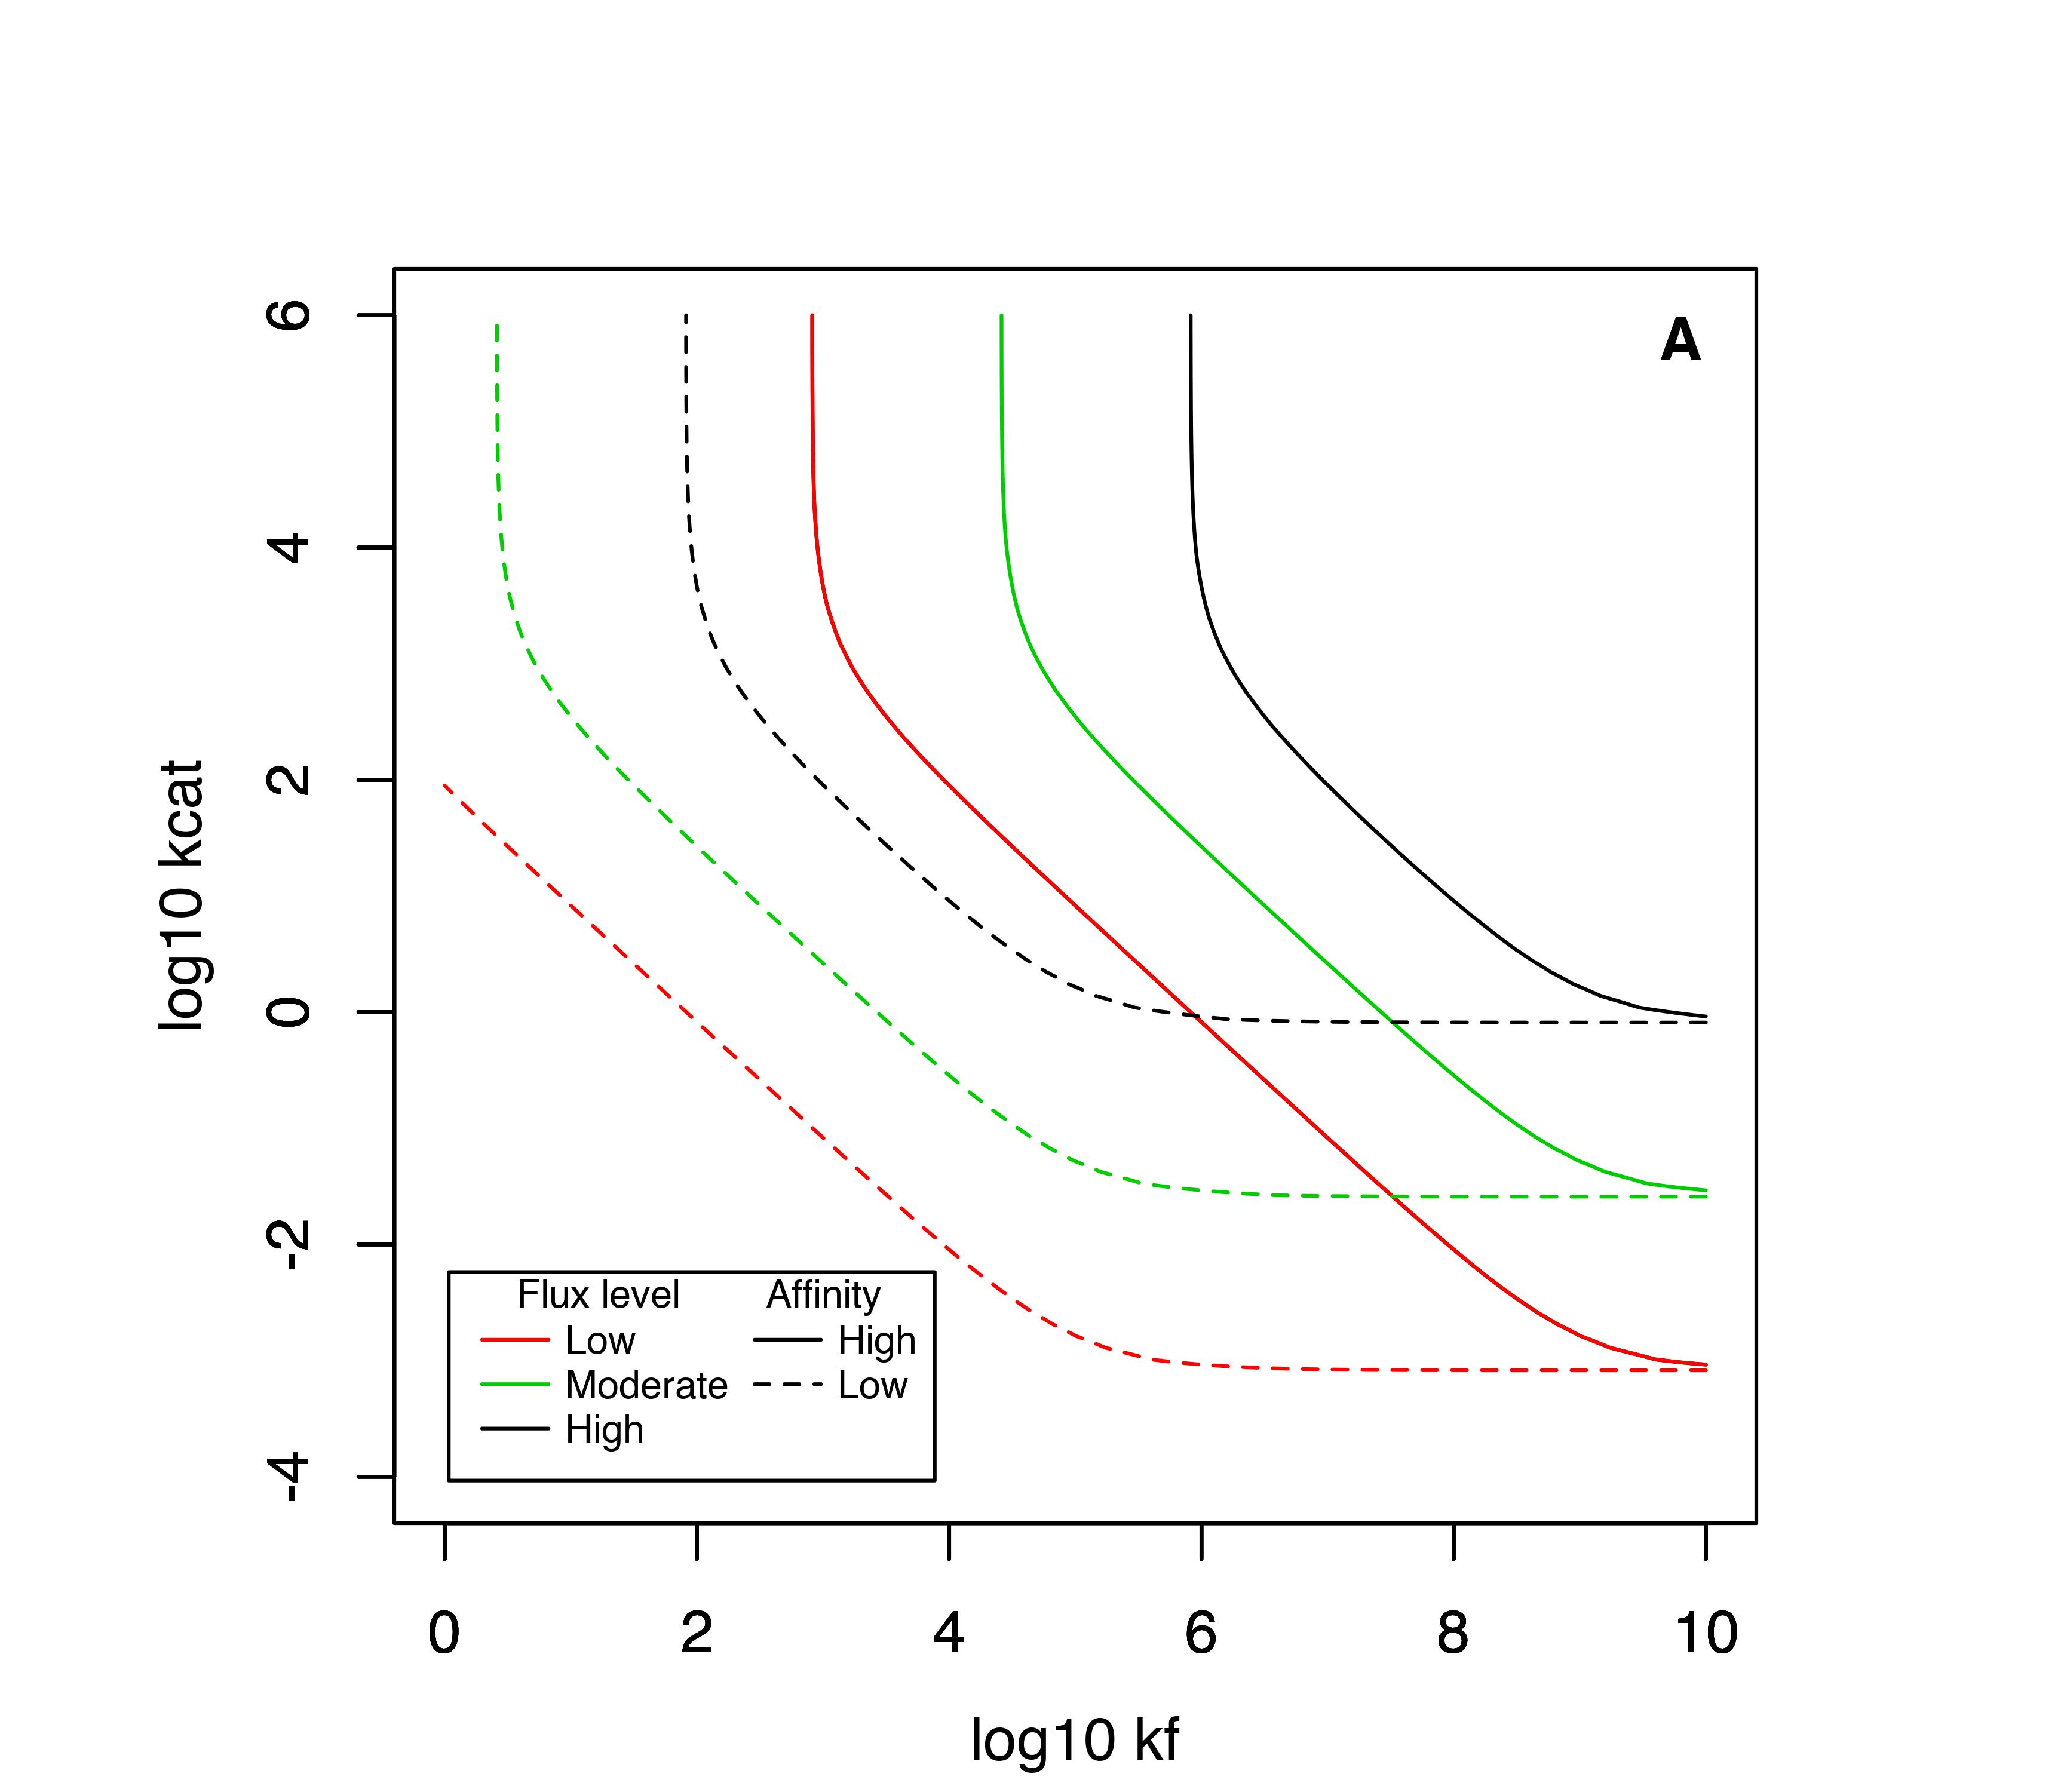
\includegraphics[scale=0.55,trim=0.5cm -0.3cm 0cm 1.5cm,clip]{pics/Enzymes/2DFit_Flux_Sat.jpeg}
%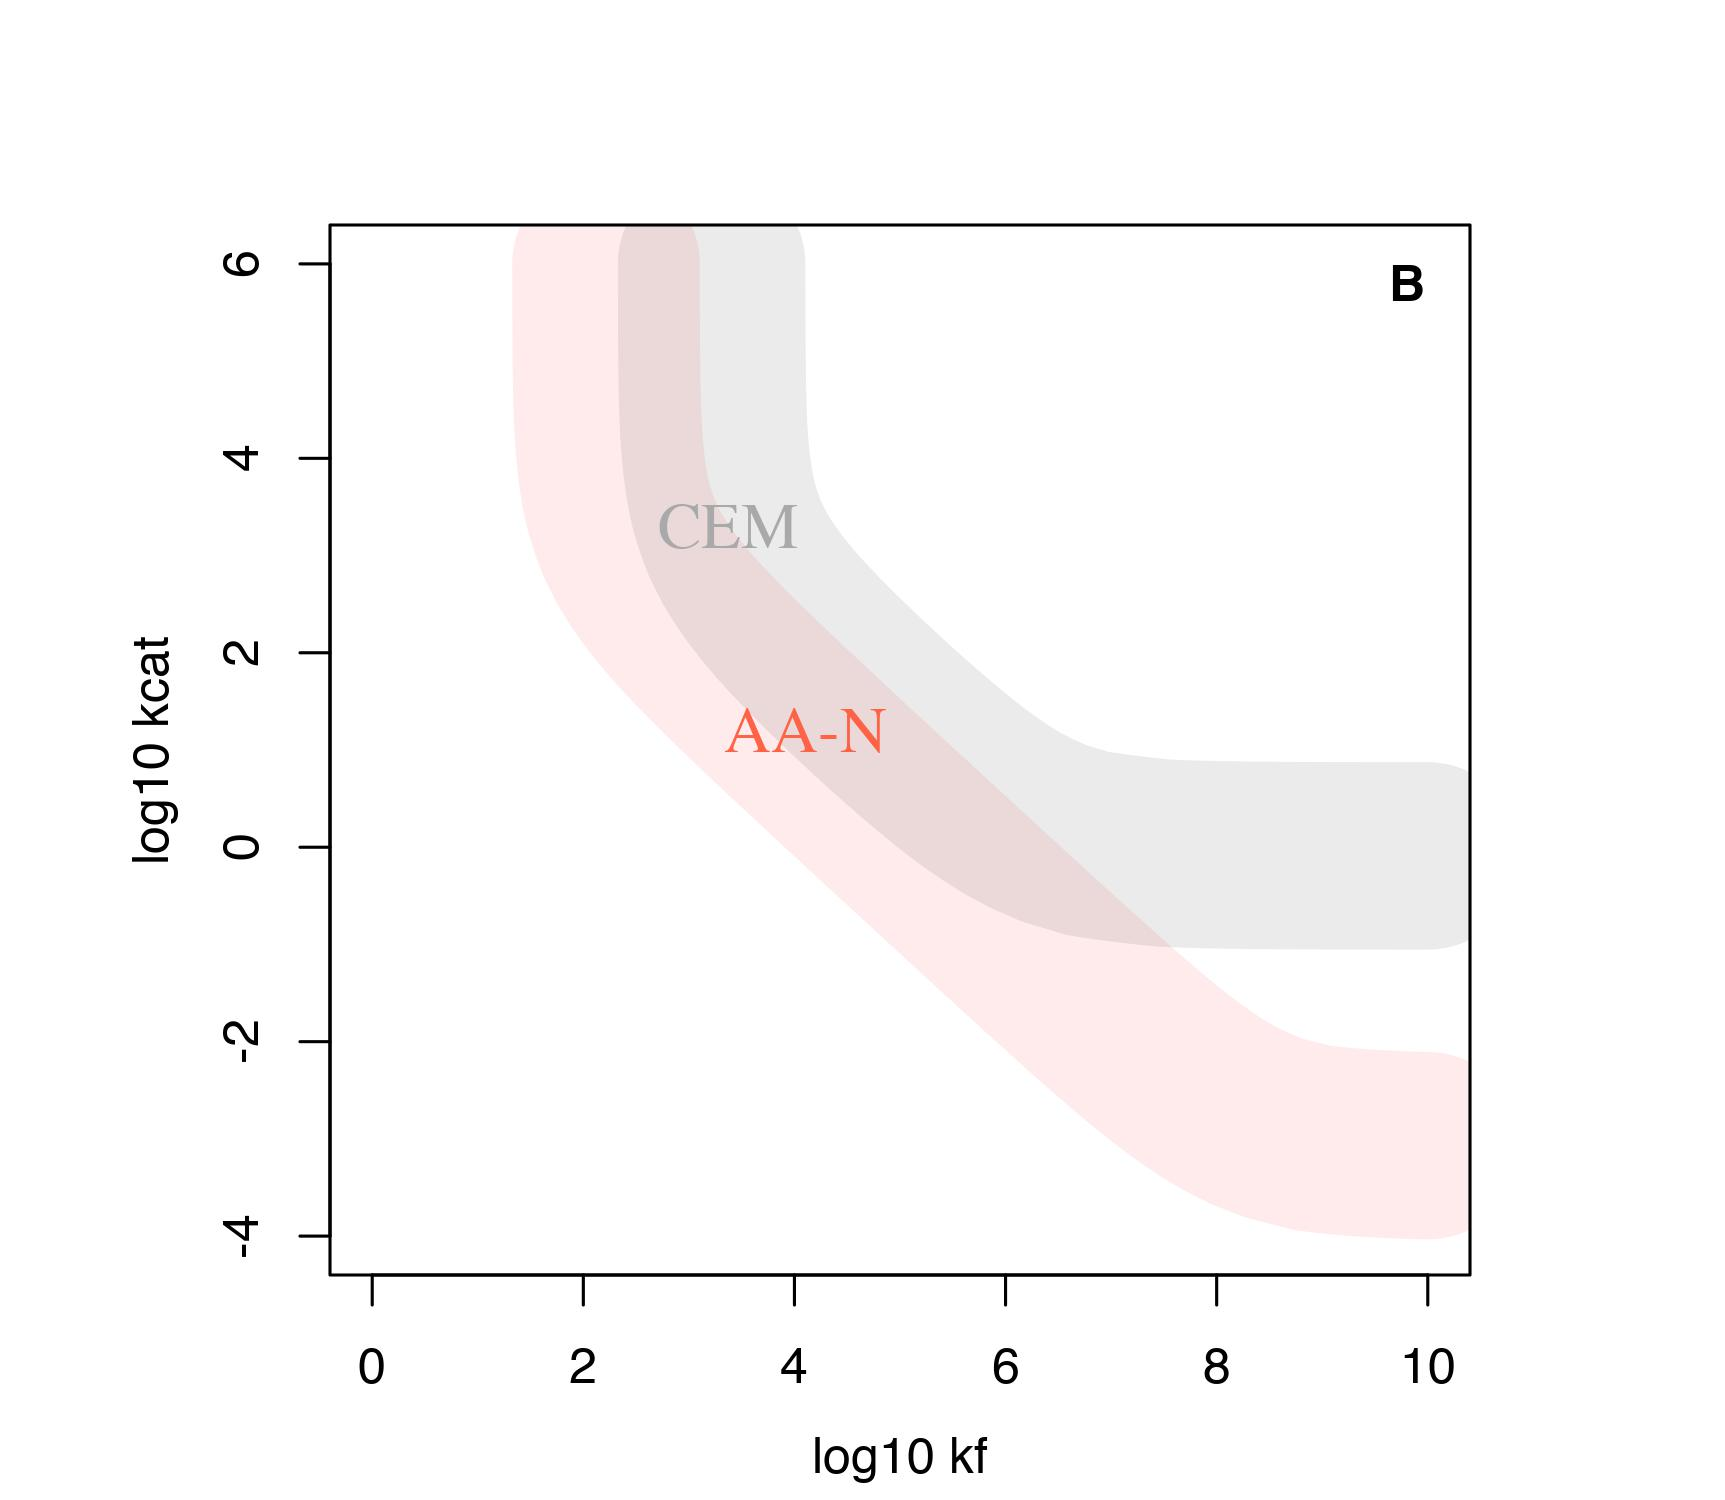
\includegraphics[scale=0.575,trim=0.5cm -0.3cm 0cm 1.5cm,clip]{Figures/2DFit_Flux&Trans.jpeg}
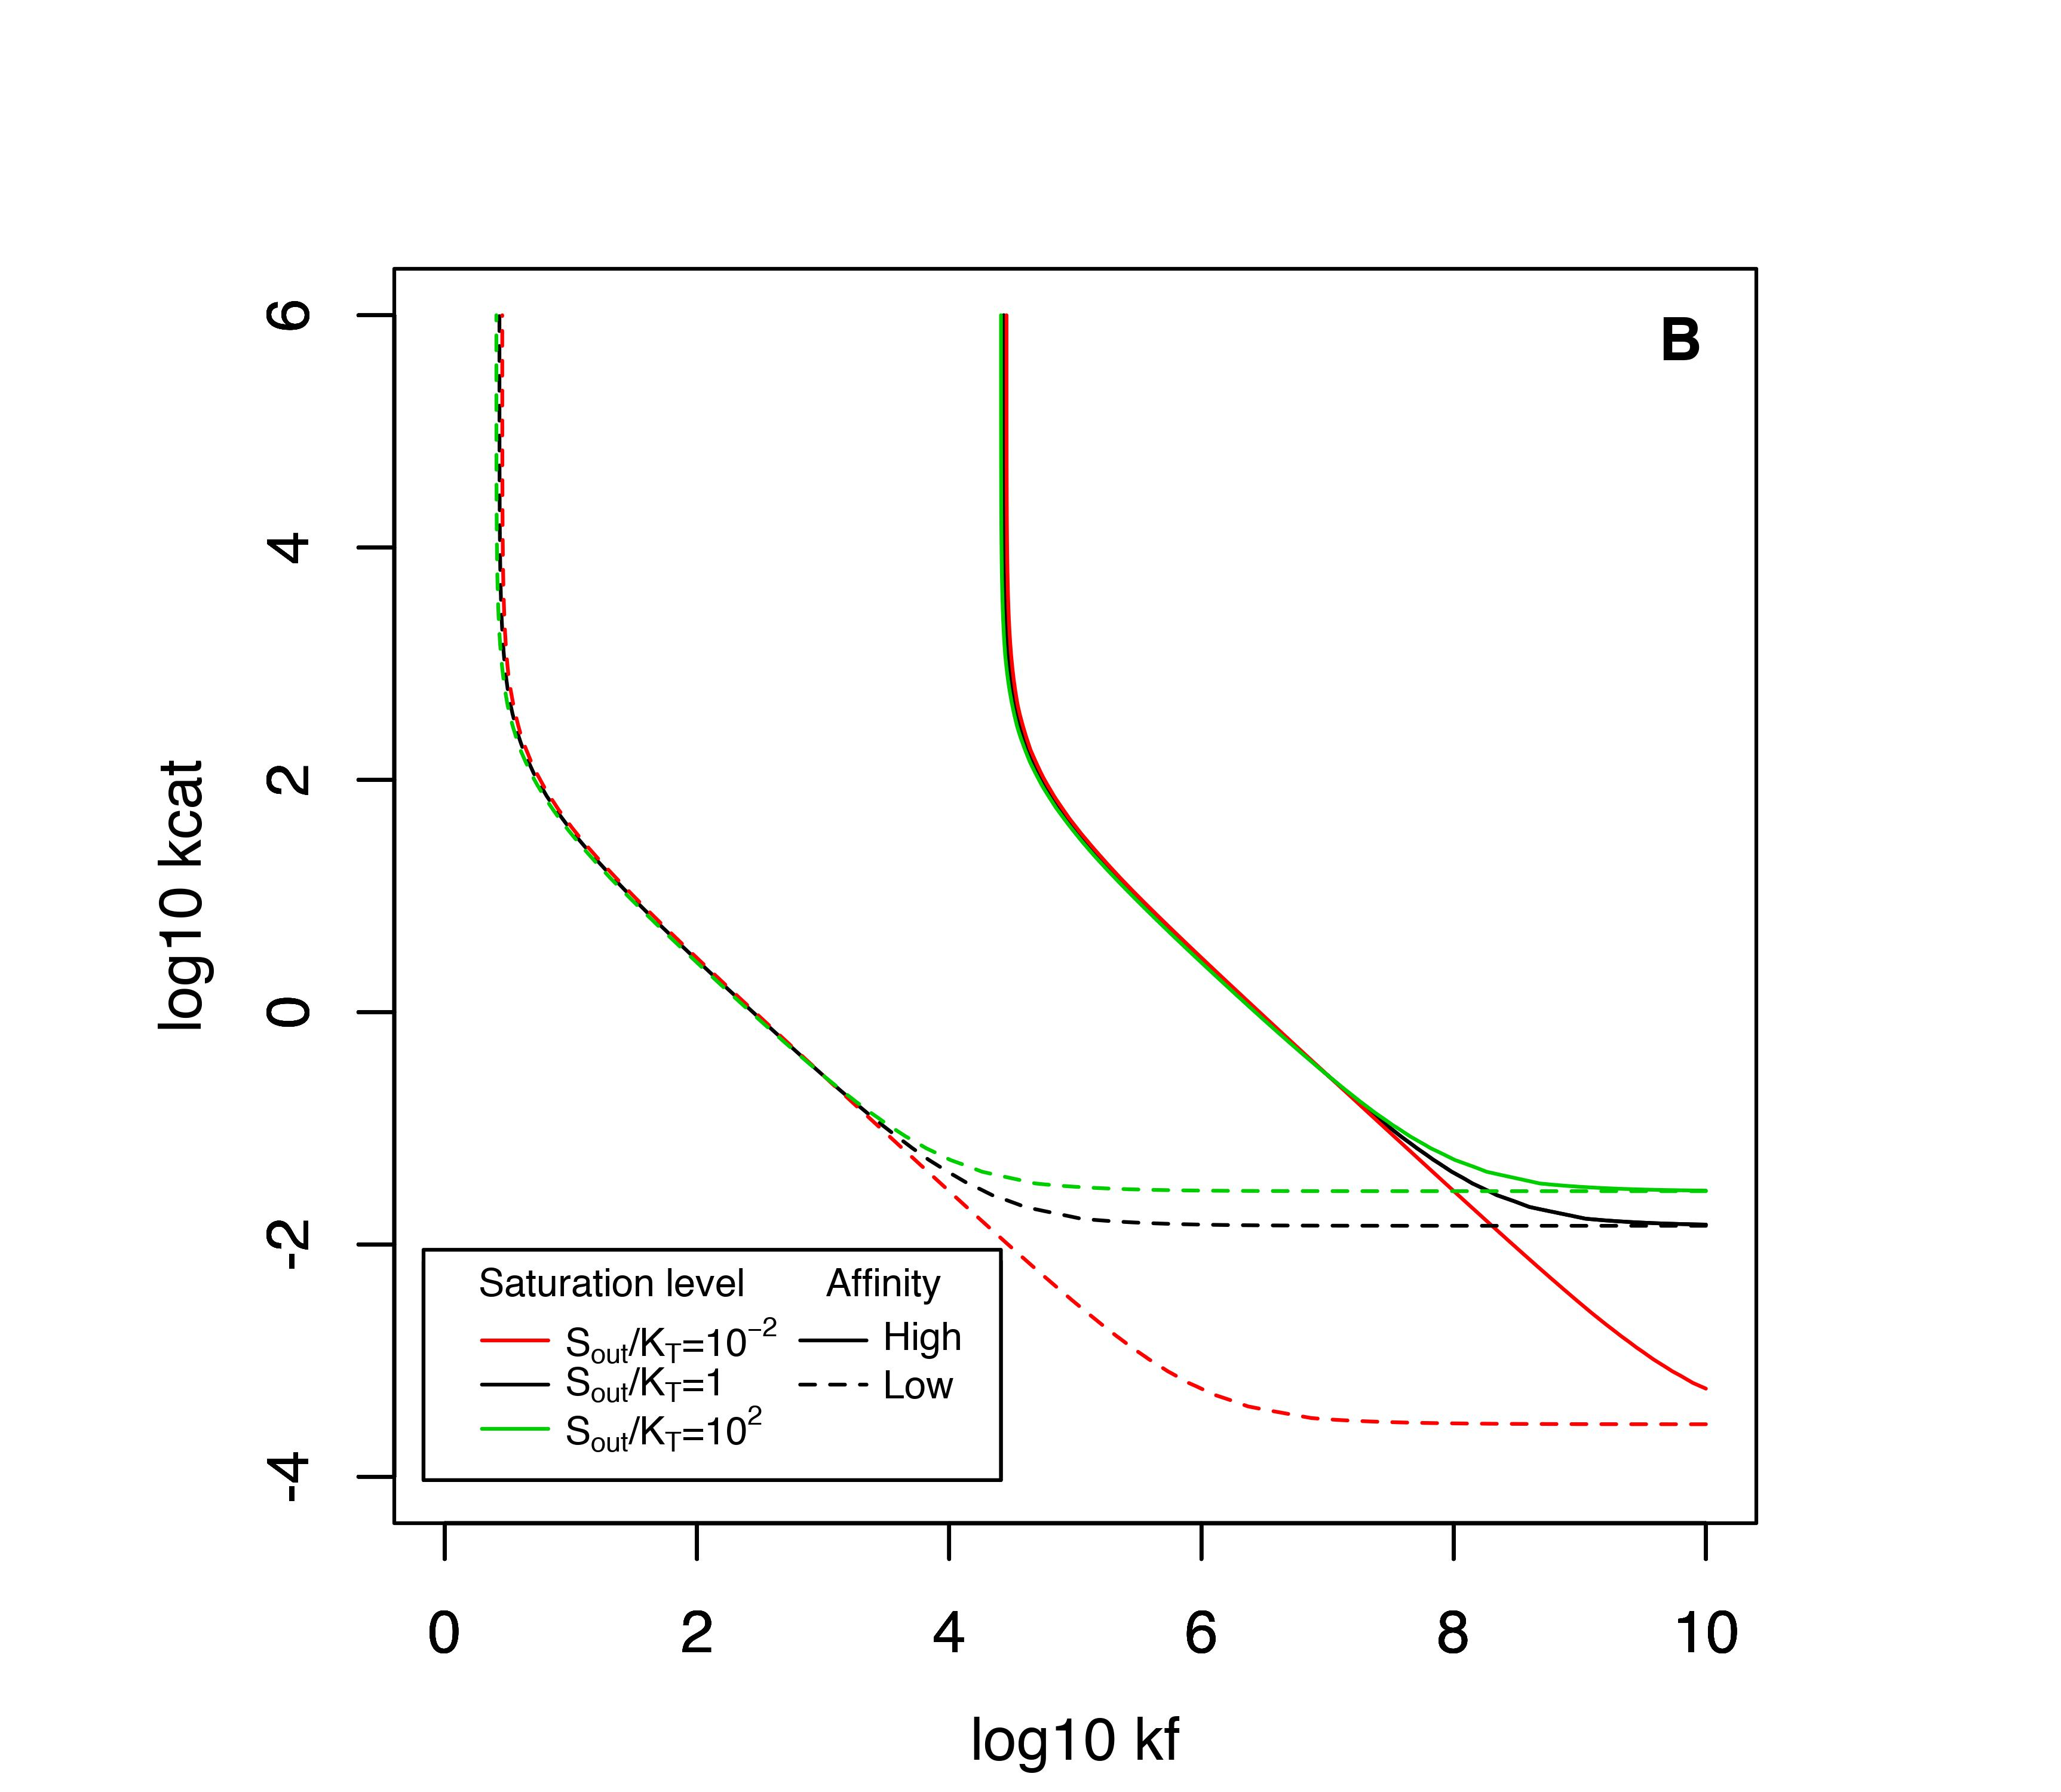
\includegraphics[scale=0.55,trim=0.5cm -0.3cm 0cm 1.5cm,clip]{pics/Enzymes/2DFit_NonSatToSat.jpeg}
%\end{minipage}
%\hfill
%\begin{minipage}{0.45\textwidth}
%\othercaption{}
%\end{minipage}
%\vspace{0.5cm}
\caption{Features of a transporter have an impact on the flux landscape for upstream enzymes, as shown by the $0.9$ isoclines -- above which the relative flux is $>90\%$ -- that delineate the fitness plateau for each set of parameter. A: low ($K_T=0.1M$) and high ($10\mu M$) transporter affinities are considered, in combination with low ($V_{Tm}=10^{-6} M$), moderate ($10^{-4.5} M$) or high maximum flux ($10^{-3} M$). Increasing $K_T$ extends the plateau only towards the left part of the landscape, allowing enzymes with lower $k_f$ on the plateau, whereas decreasing $V_{Tm}$ extends the plateau in both directions. B: the shape of the fitness plateau is however little dependent on the saturation of the transporter, for a transporter with moderate flux ($V_{Tm}=10^{-4.5}M.s^{-1}$; the effect is identical for higher $V_{Tm}$, see SM Fig. S2). Other parameter values: $k_r=1000/s$, $[E_{tot}]=1mM$ and $[S_{env}]=10 \times K_T$.}
\label{figure2DSSatStud}
\end{figure*}

So far we have considered transporters saturated by high external substrate concentrations. Relaxing this assumption has little impact on the fitness landscape, except that very low values of $k_\text{cat}$ (lower than $10^{-2}$ in FIG. \ref{figure2DSSatStud}-B) can only sustain the low influx of transporters far from saturation, but fail to keep up with higher influxes in richer environments. 
%(see Fig.~\ref{figure2DSSatStud}-B, and more in depth-explanations of this effect in the next section and in SM Text S3.1 where non saturated transporters can be assimilated to a less efficient firs enzyme). 

\noindent \paragraph{Enzymes differ among metabolic pathways}

\begin{figure}[h!]
\centering
%\includegraphics[scale=0.43,trim=0cm -0.75cm 0cm 1.5cm,clip]{Figures/2DFitLandscape_Full_Dataset.jpeg}
%\hspace{-0.3cm}
\begin{minipage}[c]{0.5\textwidth}
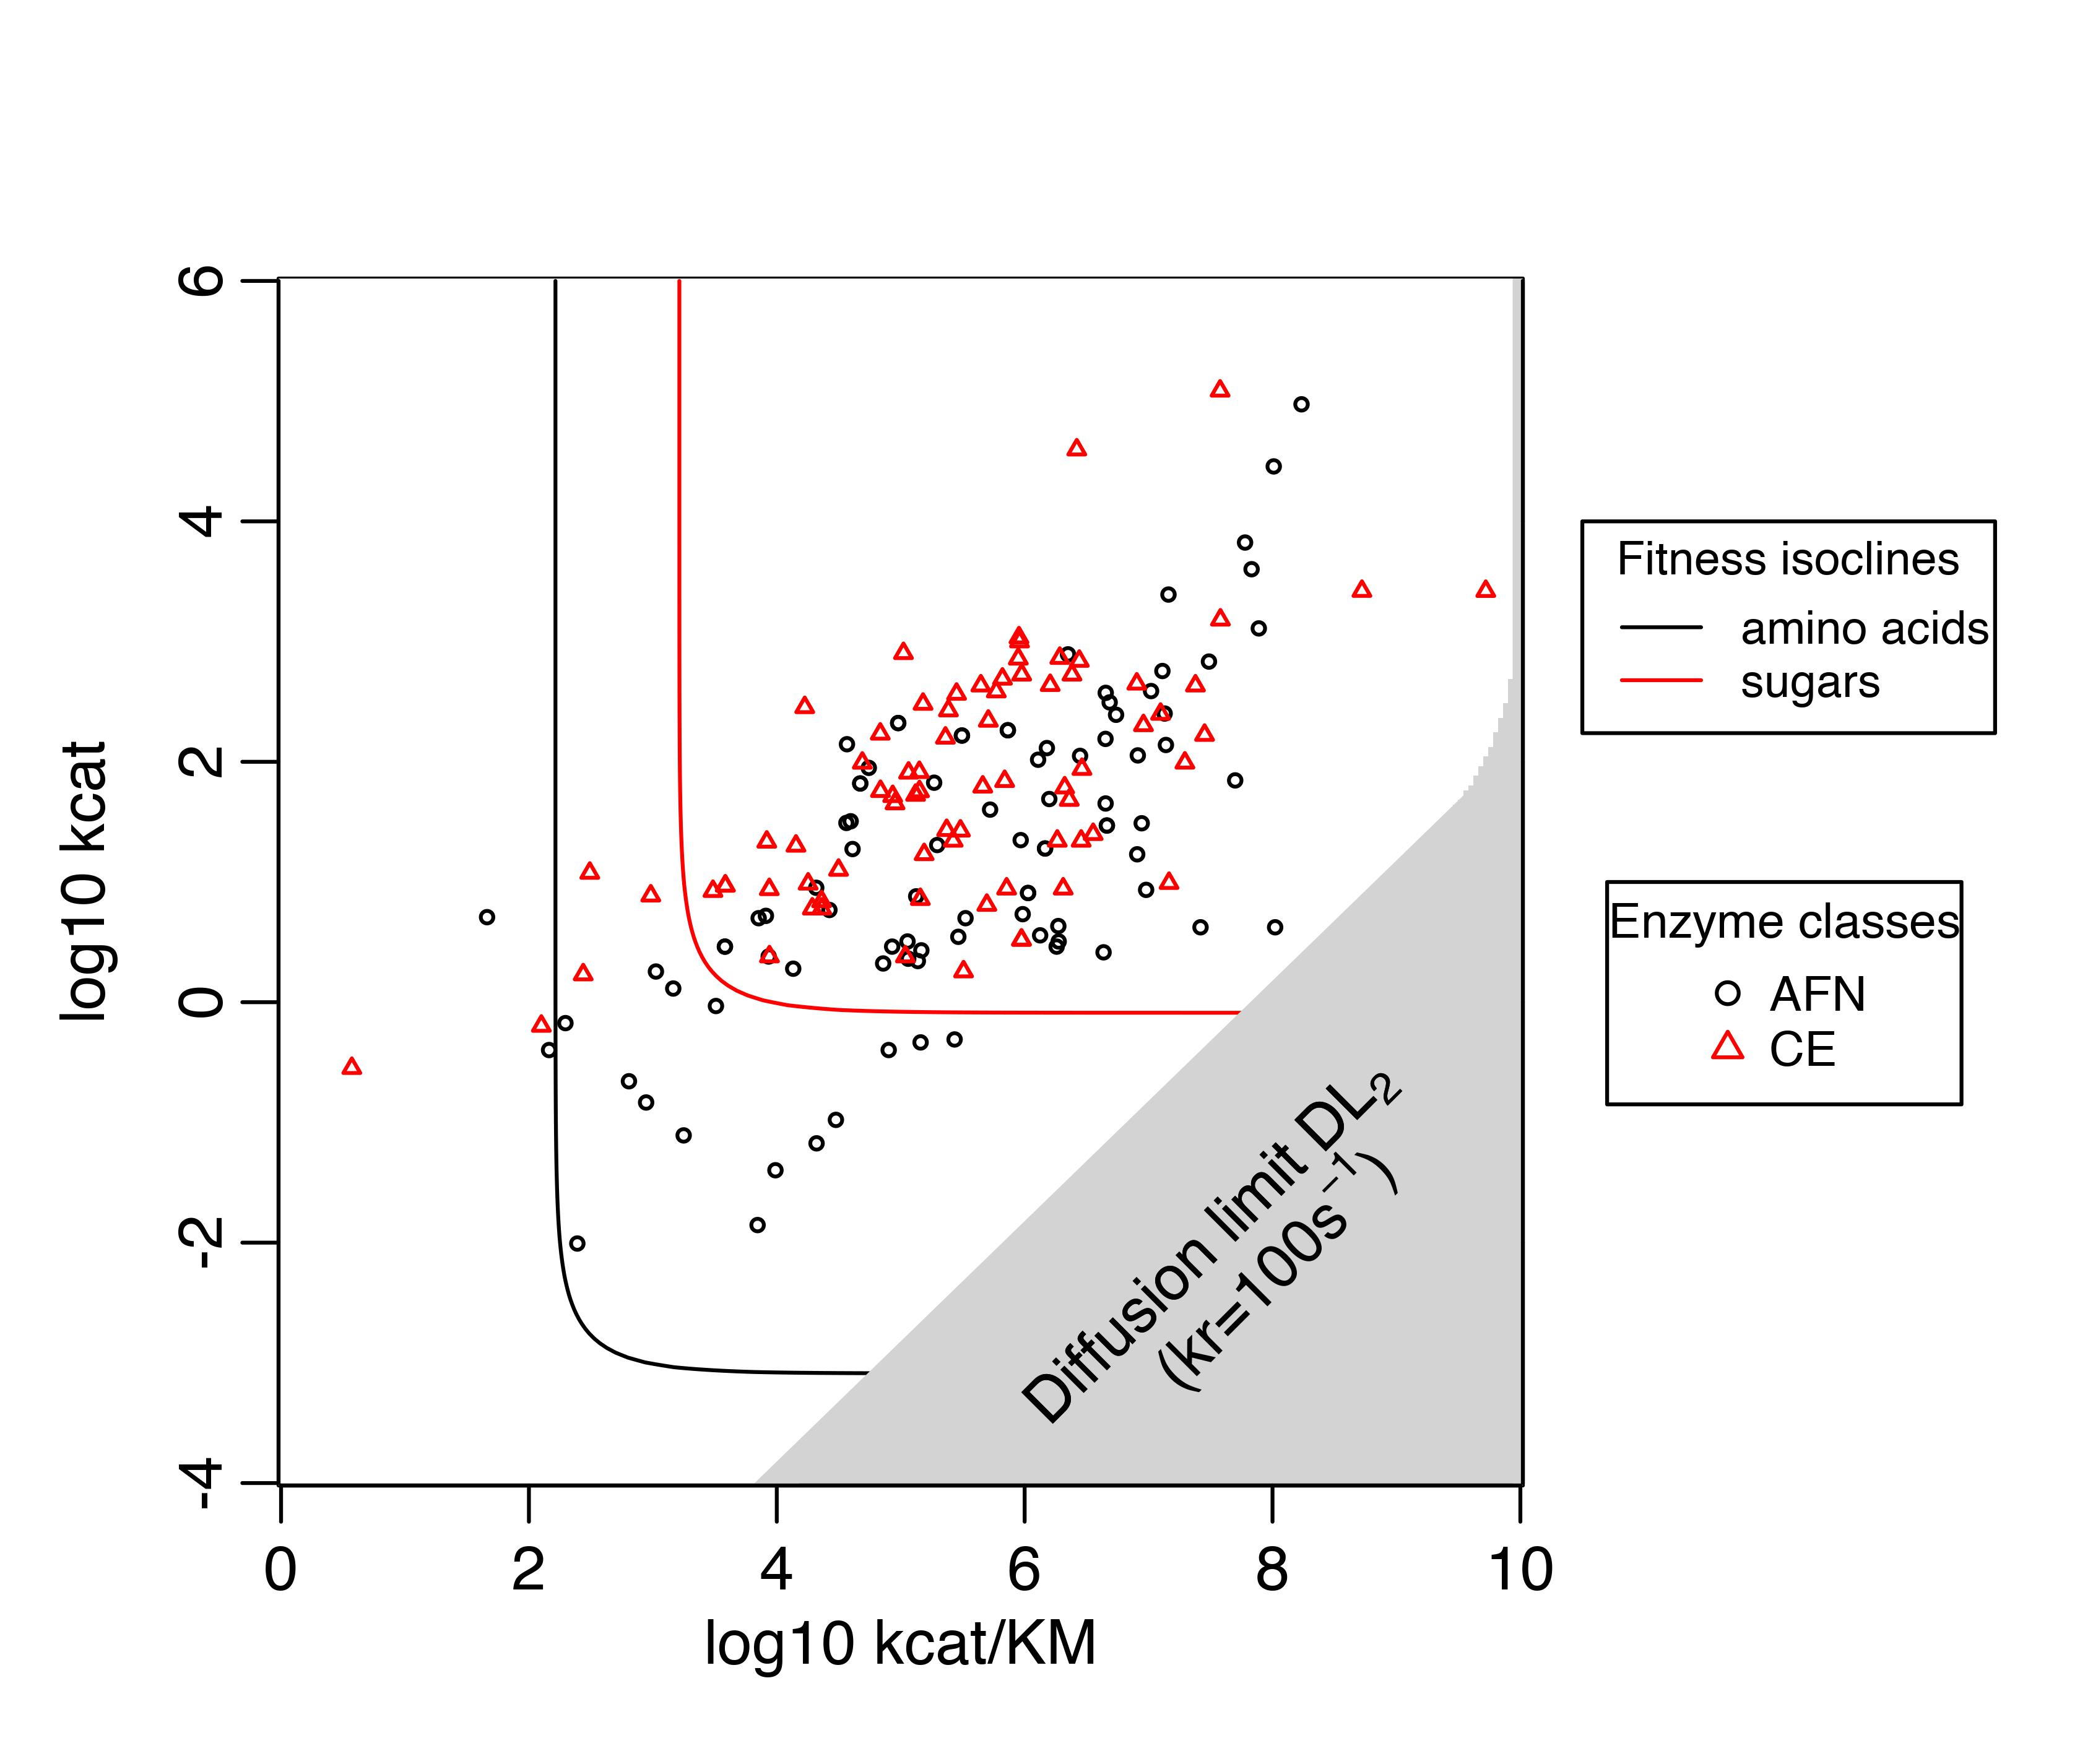
\includegraphics[scale=0.65,trim=0cm 0cm 0cm 1cm,clip]{pics/Enzymes/2DFitContour_DataClasses.jpeg}
\vspace{-0.5cm}
\caption{\textit{In vitro} experimental estimates of kinetic parameters $k_\text{cat}$ and $k_\text{cat}/K_\text{M}$ exhibit different dist-}
\label{figure2D_BarEven_Dataset}
\end{minipage}\hfill
%
\begin{minipage}[c]{0.38\textwidth}
\caption*{ributions for enzymes involved in different categories of pathways -- as identified by \citet{Bar-Even11} -- namely (AFN): amino acids, fatty acids, and nucleotides and (CE): carbohydrates and energy. Corresponding fitness landscapes -- differing by transporter features -- are superimposed, with the parameter space narrowed down due to the diffusion limit (grey area, set for $k_r=10^2 s^{-1}$). The isoclines shown correspond to parameter values typical of sugar transporters ($K_T=5mM$,$V_{Tm}=1mM.s^{-1}$, in red) \citep{Maier02} or amino acids transporters (same as in FIG.~\ref{figure3D2DFit}, in black).}
\end{minipage}
\end{figure}

We then superimposed empirical estimates of kinetic parameters over our theoretical fitness landscapes, after substituting parameter $k_f$ for its usual empirical counterpart, $k_\text{cat} / K_\text{M}$. Because $k_{cat}/K_\text{M} = k_fk_{cat}/(k_r+k_{cat})$, this approximation only holds when $k_\text{cat} \gg k_r$. Representing the fitness landscape in this parameter space
sets an inaccessible area in the bottomright part of the landscapes where $k_f$ would exceed the diffusion limit (grey area on FIG.~\ref{figure2D_BarEven_Dataset}). For purposes of inclusiveness, we used $k_r=10^{2}s^{-1}$ by default -- noting that this limit would be displaced upwards for larger $k_r$ (and downwards otherwise).

We otherwise used sets of parameters that correspond to typical features of sugar and amino acid/nucleoside transporters to obtain FIG.~\ref{figure2D_BarEven_Dataset}. Because we have previously shown that changing the affinity or maximum flux of transporters may move the fitness plateau, our model predicts that enzymes involved in the corresponding pathways (\textit{e.g.} of sugars and amino acids) should have their own specific distributions. We see that enzymes involved in the central carbohydrate metabolism as categorized by \citet{Bar-Even11} have on average higher $k_\text{cat}$ and $K_\text{M}$ than those metabolising amino-acids and nucleotides. Our superimposition with the predicted fitness plateaus in FIG.~\ref{figure2D_BarEven_Dataset} suggests that there may indeed be an explainable difference between enzymes contributing to carbohydrate processing (in red) and to that of other primary metabolites (in black, \textit{e.g.} amino acids).
We acknowledge that this result implicitly suggests that enzymes within a pathway have evolved on a common fitness landscape, spreading neutrally onto the fitness plateau. This is by no means our interpretation, as this subset of the full dataset includes enzymes that differ in many other ways that, as we will see, make each enzyme evolve on its own fitness landscape and thereby potentially explain a large part of this observed variance. 

\noindent \paragraph{Downstream enzymes also evolve on cliff-like fitness landscapes}

\begin{figure*}[t!]
\centering
\begin{minipage}[c]{0.48\linewidth}
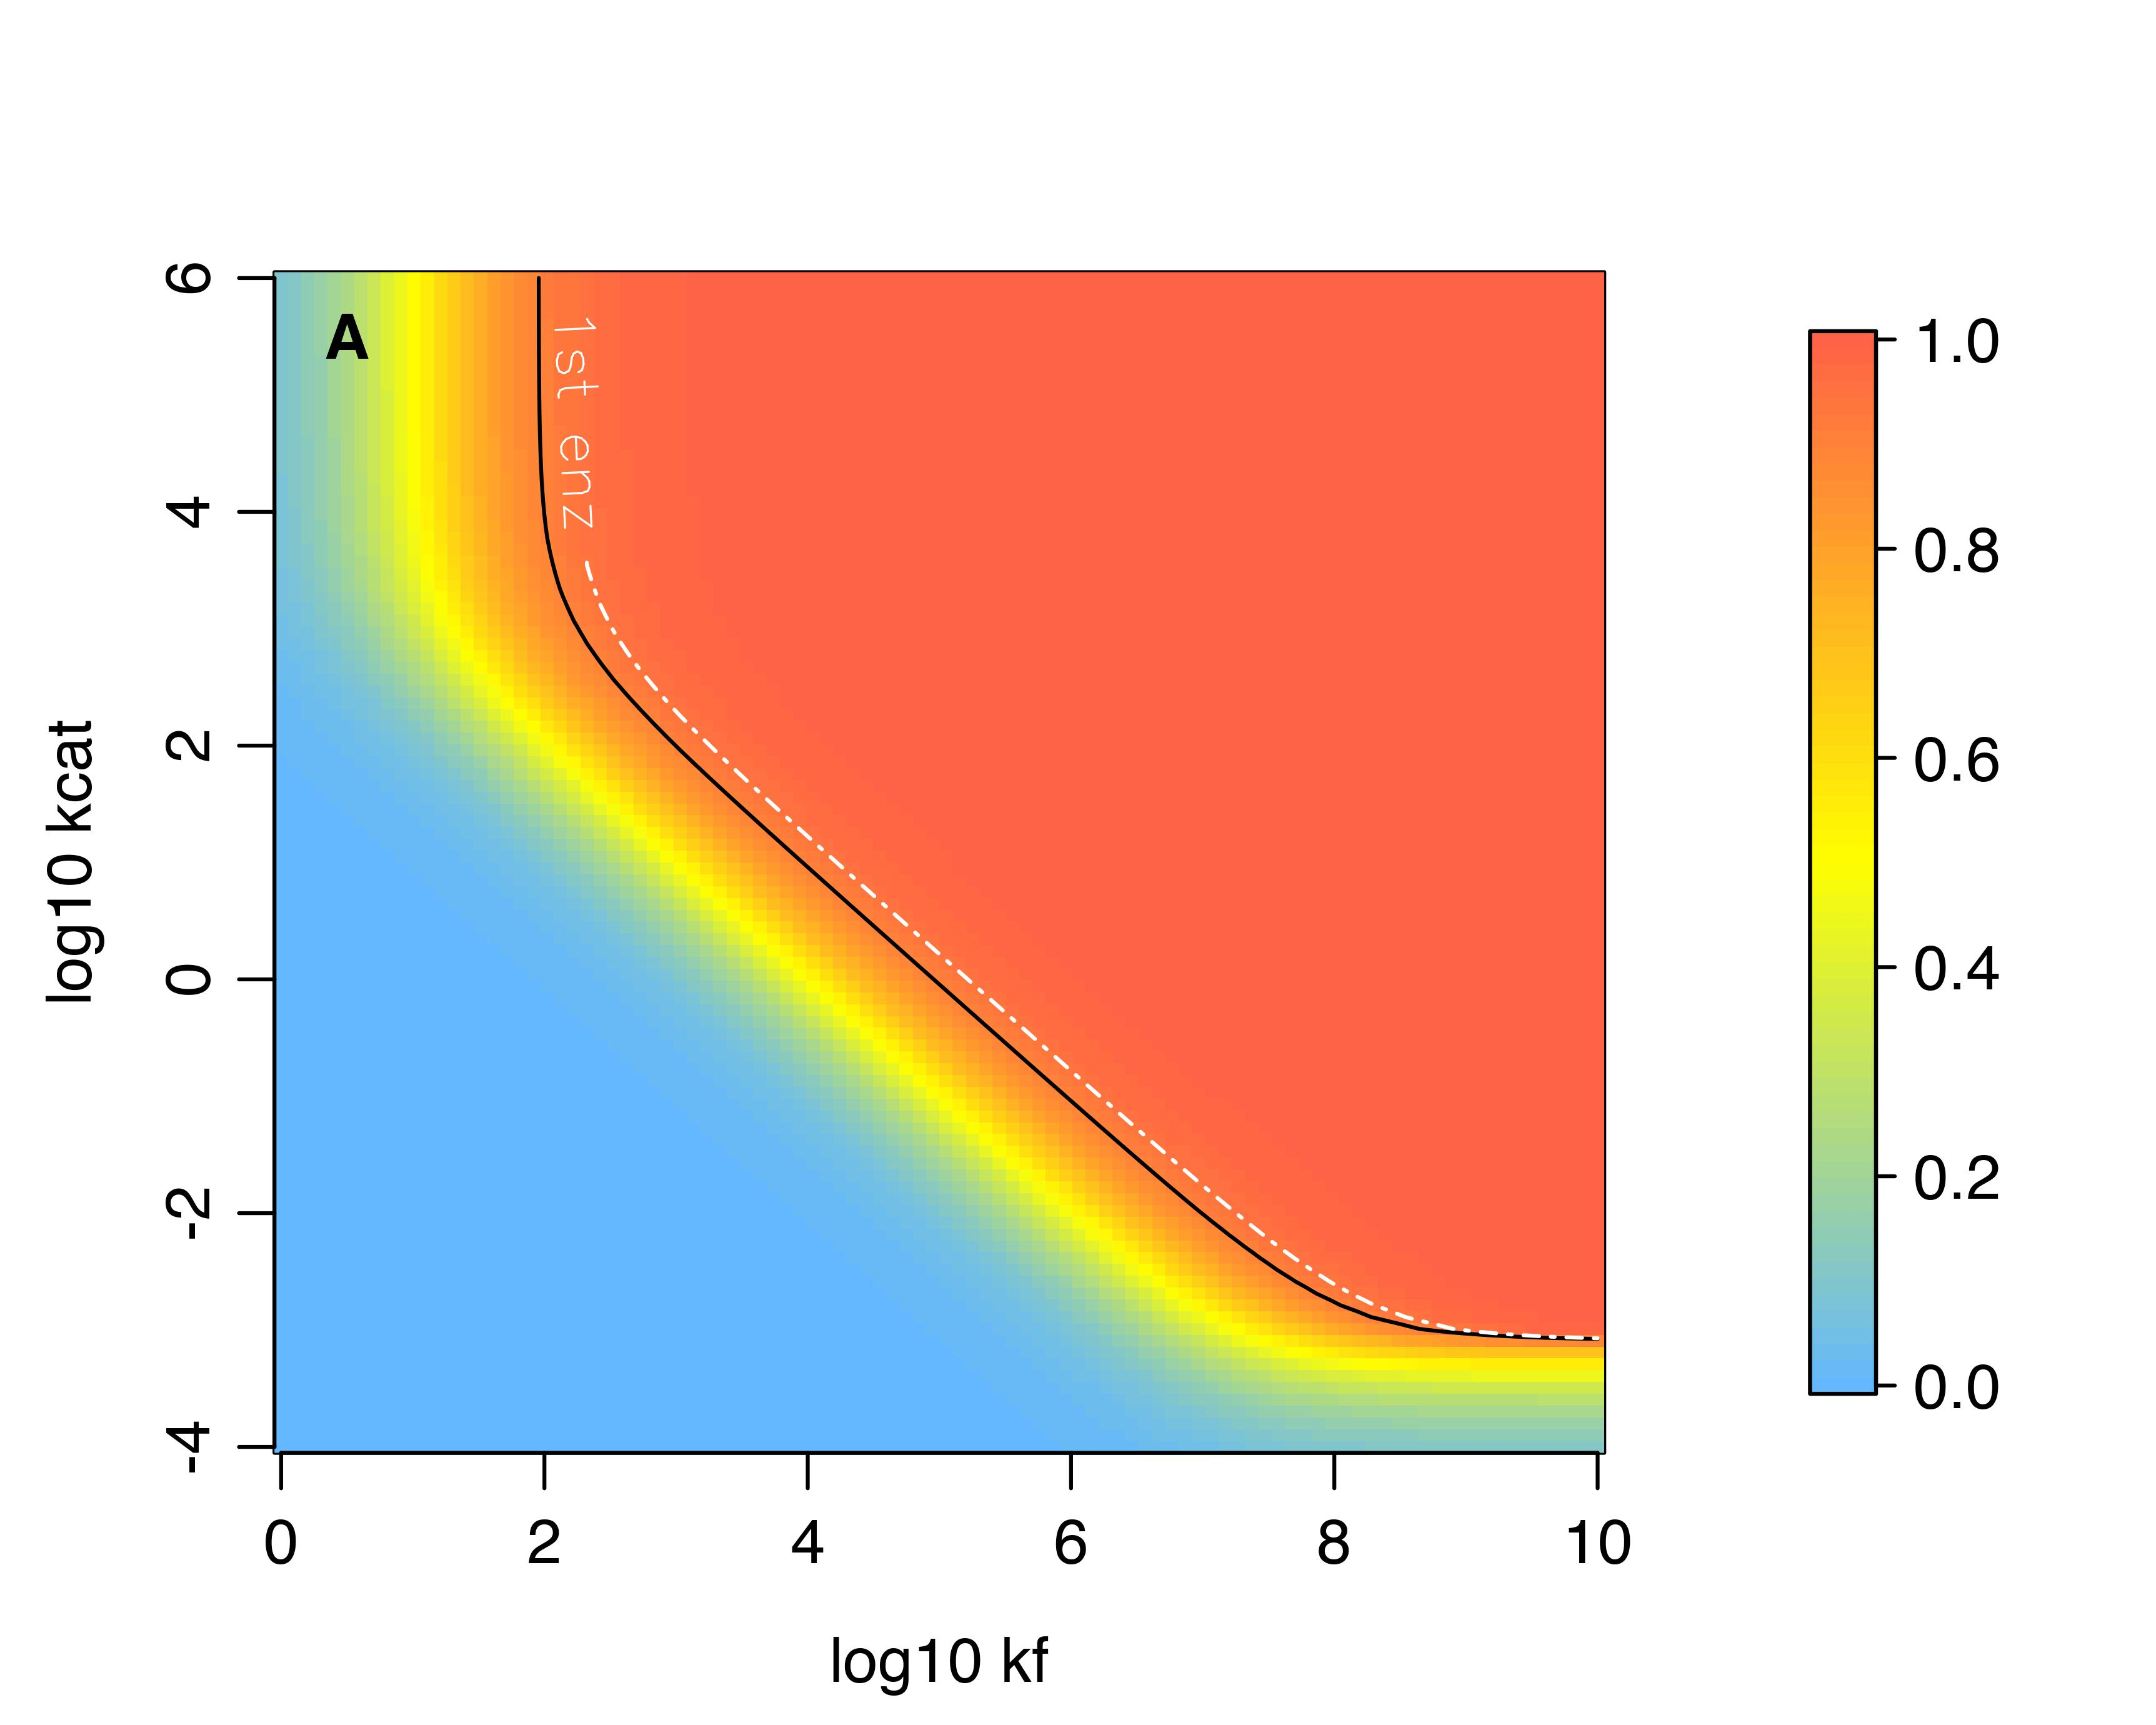
\includegraphics[scale=0.625,trim=0cm 0cm 0cm 1.5cm,clip]{pics/Enzymes/2DFitLandscape_etahigh_noreverse.jpeg} 
%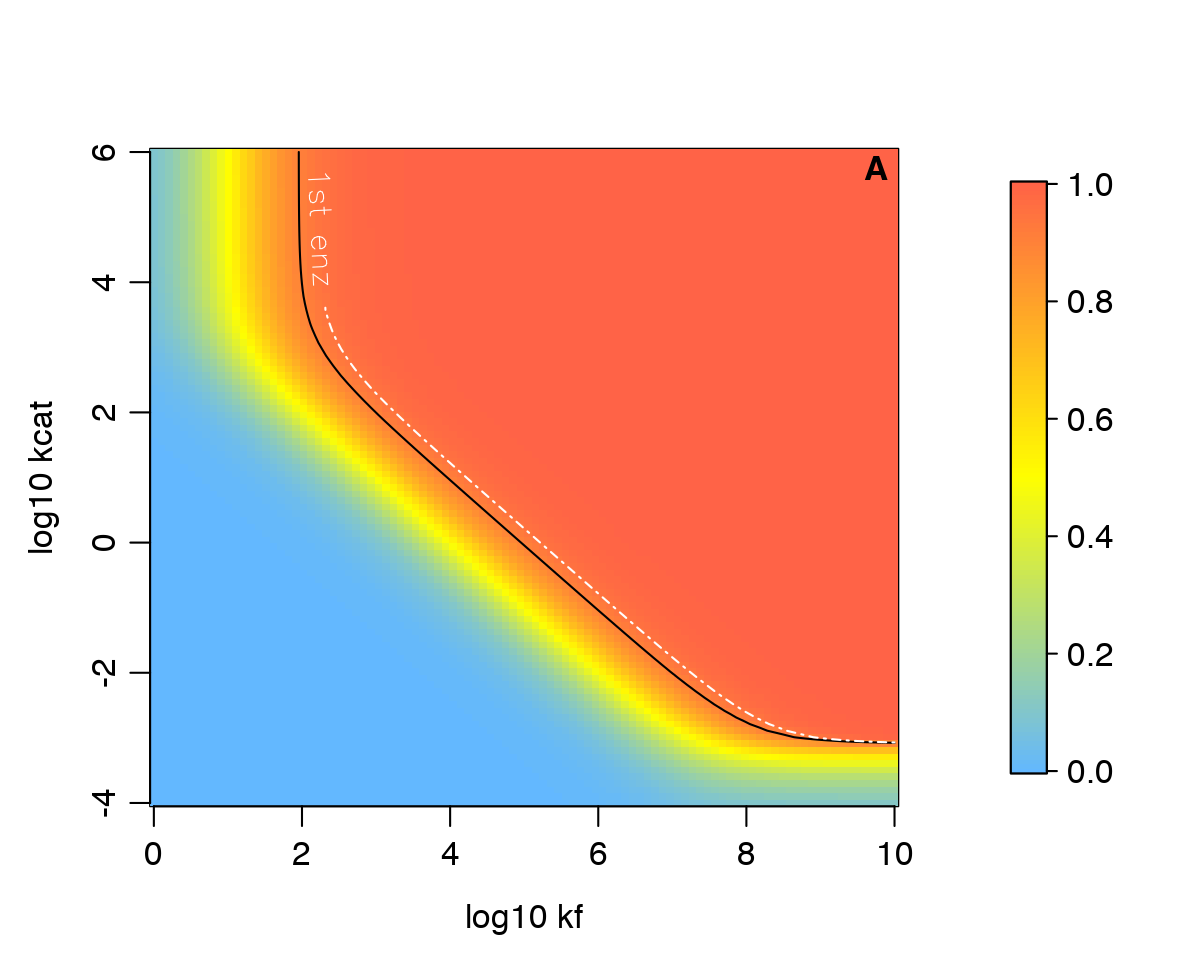
\includegraphics[scale=0.5]{Figures/2DFitLandscape_etahigh_noreverse.png} 
\end{minipage} \hfill
\begin{minipage}[c]{0.48\linewidth}
\includegraphics[scale=0.625,trim=0cm 0cm 0cm 1.5cm,clip]{pics/Enzymes/2DFit_Landscape_2Enz_First_Enz_Influence.jpeg} 
%\includegraphics[scale=0.42,trim=10 0 0 0,clip]{Figures/2DFit_Landscape_2Enz_First_Enz_Influence.jpeg} 
\end{minipage}
%\vspace{0.5cm}
\caption{Downstream enzymes exhibit similar fitness landscapes as those upstream, with a dependency to degradation parameter $\eta_d$. A: a high degradation rate ($\eta_d=10^{-2} /s$) results in a fitness plateau for the second enzyme very similar to that of the first enzyme ; in the case presented the first enzyme is considered ``perfect'' in order to draw the fitness landscape of the second enzyme ($k_f=10^{10}M^{-1}.s^{-1}$, $k_{cat}=10^6s^{-1}$, $k_r=10^3s^{-1}$, $[E_{tot}]=1mM$). B: decreasing the degradation rate allows less efficient enzymes (with lower $k_\text{cat}$ or $k_f$) to reach the fitness plateau. Considering the first enzyme to be inefficient ($k_f=10^{2}M^{-1}.s^{-1}$, $k_{cat}=10^{-2}s^{-1}$, $k_r=10^3s^{-1}$) instead of perfect marginally changes the fitness landscape by making organisms tolerant to extremely low $k_\text{cat}$. Other parameter values are identical to FIG.~\ref{figure3D2DFit} (findings are relatively similar for sugar-like transporters, as reported in SM - Fig. S6).}
\label{figure2D_2Enz_Deg}
\end{figure*}

One of the factors that makes enzymes different along a pathway is their position, such that the fitness landscape in FIG.\ref{figure3D2DFit} may only hold for the most upstream enzyme in a pathway. Indeed, because the flux of the first product in a pathway increases with the substrate gradient across the cell membrane, the upstream enzyme of a given metabolic pathway is selected for efficiency as described above. In contrast, this selection pressure does not apply directly downstream; at steady-state, even inefficient enzymes can in principle process newly formed substrate molecules at an elevated rate, assuming that the concentration of the substrate is allowed to reach any steady-state value. This is an obviously unreasonable assumption, since a part of this standing substrate should be lost by outward diffusion or degradation \citep{Jones15,Bosdriesz18}. The loss of fitness may therefore result from the loss of metabolites in a way that can be modelled by a constant degradation rate $\eta_{d}$ \citep{Chou14} (assuming that the external environment is infinite, the degradation term can as well represent an efflux). Highly concentrated metabolites may also be involved in widespread non-specific \citep{Keller15} or promiscuous interactions \citep{Khersonsky10,Schauble13,Peracchi18} that may interfere with other cellular processes; this is well captured by the linear cost as non-specific interactions should follow Michaelis-Menten kinetics albeit with much lower affinities, hence following an approximately linear relationship up to very high cellular concentrations (see Materials and Methods for more details). However for some reactions the accumulation of metabolites may result in the production of toxic compounds \citep{Lilja17, Niehaus20}, hence triggering toxicity best modelled as a non-linear fitness cost \citep{Clark91,Wright10}.

We first consider a ``perfect", highly concentrated upstream enzyme ($k_f=10^{10}M^{-1}s^{-1}$, $k_{cat}=10^6s^{-1}$, $k_r=10^3s^{-1}$, $[E_{tot}]=10^{-3}M$) and focus on the second enzyme in the pathway, showing that it evolves on a fitness landscape that has a similar shape than described above, still hitting a plateau (FIG.~\ref{figure2D_2Enz_Deg}, with the same parameterization as FIG.~\ref{figure3D2DFit}). The degradation rate creates a ceiling for the concentration of the product of the first reaction, such that reducing $\eta_{d}$ allows for higher concentrations (see SM Fig. S4) and makes the flux tolerant to second enzymes with lower $k_f$s, whereas selection on $k_\text{cat}$ is barely impacted by this parameter. The plateau is therefore extended to the left when high product concentrations are enabled at low $\eta_{d}$ (see FIG.~\ref{figure2D_2Enz_Deg}-B). The shape of the plateau is little impacted by changes in the efficiency of the first enzyme, especially when it stands on the plateau. These results are almost independent of the transporter initiating the pathway %, although degradation rates limiting metabolite concentrations to similar levels push the plateau to the right slightly more when compared to the landscape of the first enzyme 
(see SM Fig. S6 for the case of moderate affinity, high flux transporters). 

The shape of the negative relationship between metabolite concentration and fitness can be important (Figs~S7-S9 in SM), as it can make the fitness landscape of an enzyme dependent of the overall flux of the metabolic pathway, and therefore on other enzymes in the pathway. Indeed, low general fluxes (as modelled by an inefficient first enzyme in Figs. S7-S8) make the metabolite concentration below its toxicity threshold, therefore making organisms tolerant to enzymes with lower $k_f$ and $k_\text{cat}$. Taken together, these results show that the precise epistatic relationship between enzymes in a pathway will depend on the exact cost function applied, with a linear cost generating epistasis for $k_\text{cat}$ only and a non-linear cost possibly impacting both $k_f$ and $k_\text{cat}$.

\noindent \paragraph{The reversibility of reactions also matters}

Reversibility is an intrinsic feature of chemical reactions that cannot be directly overcome by Evolution \citep{Haldane30,Cornish-Bowden79a}. A highly reversible reaction corresponds to a large intrinsic equilibrium constant $K_{eq}=[S]_{eq}/[P]_{eq}$ \citep{Klipp94}, and results in higher backward than forward rates in the following chemical equation: \begin{equation}
\ce{ E + S <=>[k_{f}][k_{r}] ES <=>[k_{cat}][k_{inh}] E + P_1 },
\label{chemMM_fullrev}
\end{equation}
where $k_{inh}$ represents the rate at which enzyme and product combine back. Such a (reversible) reaction could in principle influence the selective pressure acting on the following enzyme in the pathway, for both enzymes compete to process the same metabolite $P_1$. We thus quantified how reversibility affects the evolution of an enzyme downstream (SM Figs S10 and S11). 

The equilibrium constant $K_{eq}$ has a similar (non-linear) impact on the fitness landscape of the second enzyme to that of the degradation rate, with a highly reversible upstream enzyme exerting a selection pressure downstream towards an increase of kinetic parameters (SM Fig. S10-A). Indeed, increasing $K_{eq}$ moves the fitness plateau toward the upper-right corner in the ($k_f$, $k_\text{cat}$) parameter space, hence selecting for more efficient downstream enzymes. The effect appears linear, except for very low values of $K_{eq}$ where metabolite accumulation exerts a dominant role in shaping the fitness landscape (through the degradation rate $\eta_d$, set to a low residual value). Therefore, the reversibility of the upstream reaction appears like a critical parameter for the evolution of an enzyme. 


\noindent \paragraph{Evolutionary dynamics of enzyme kinetic parameters}

\begin{figure*}[h!]
\centering
\begin{minipage}[c]{0.5\linewidth}
%\hspace{0.1cm}
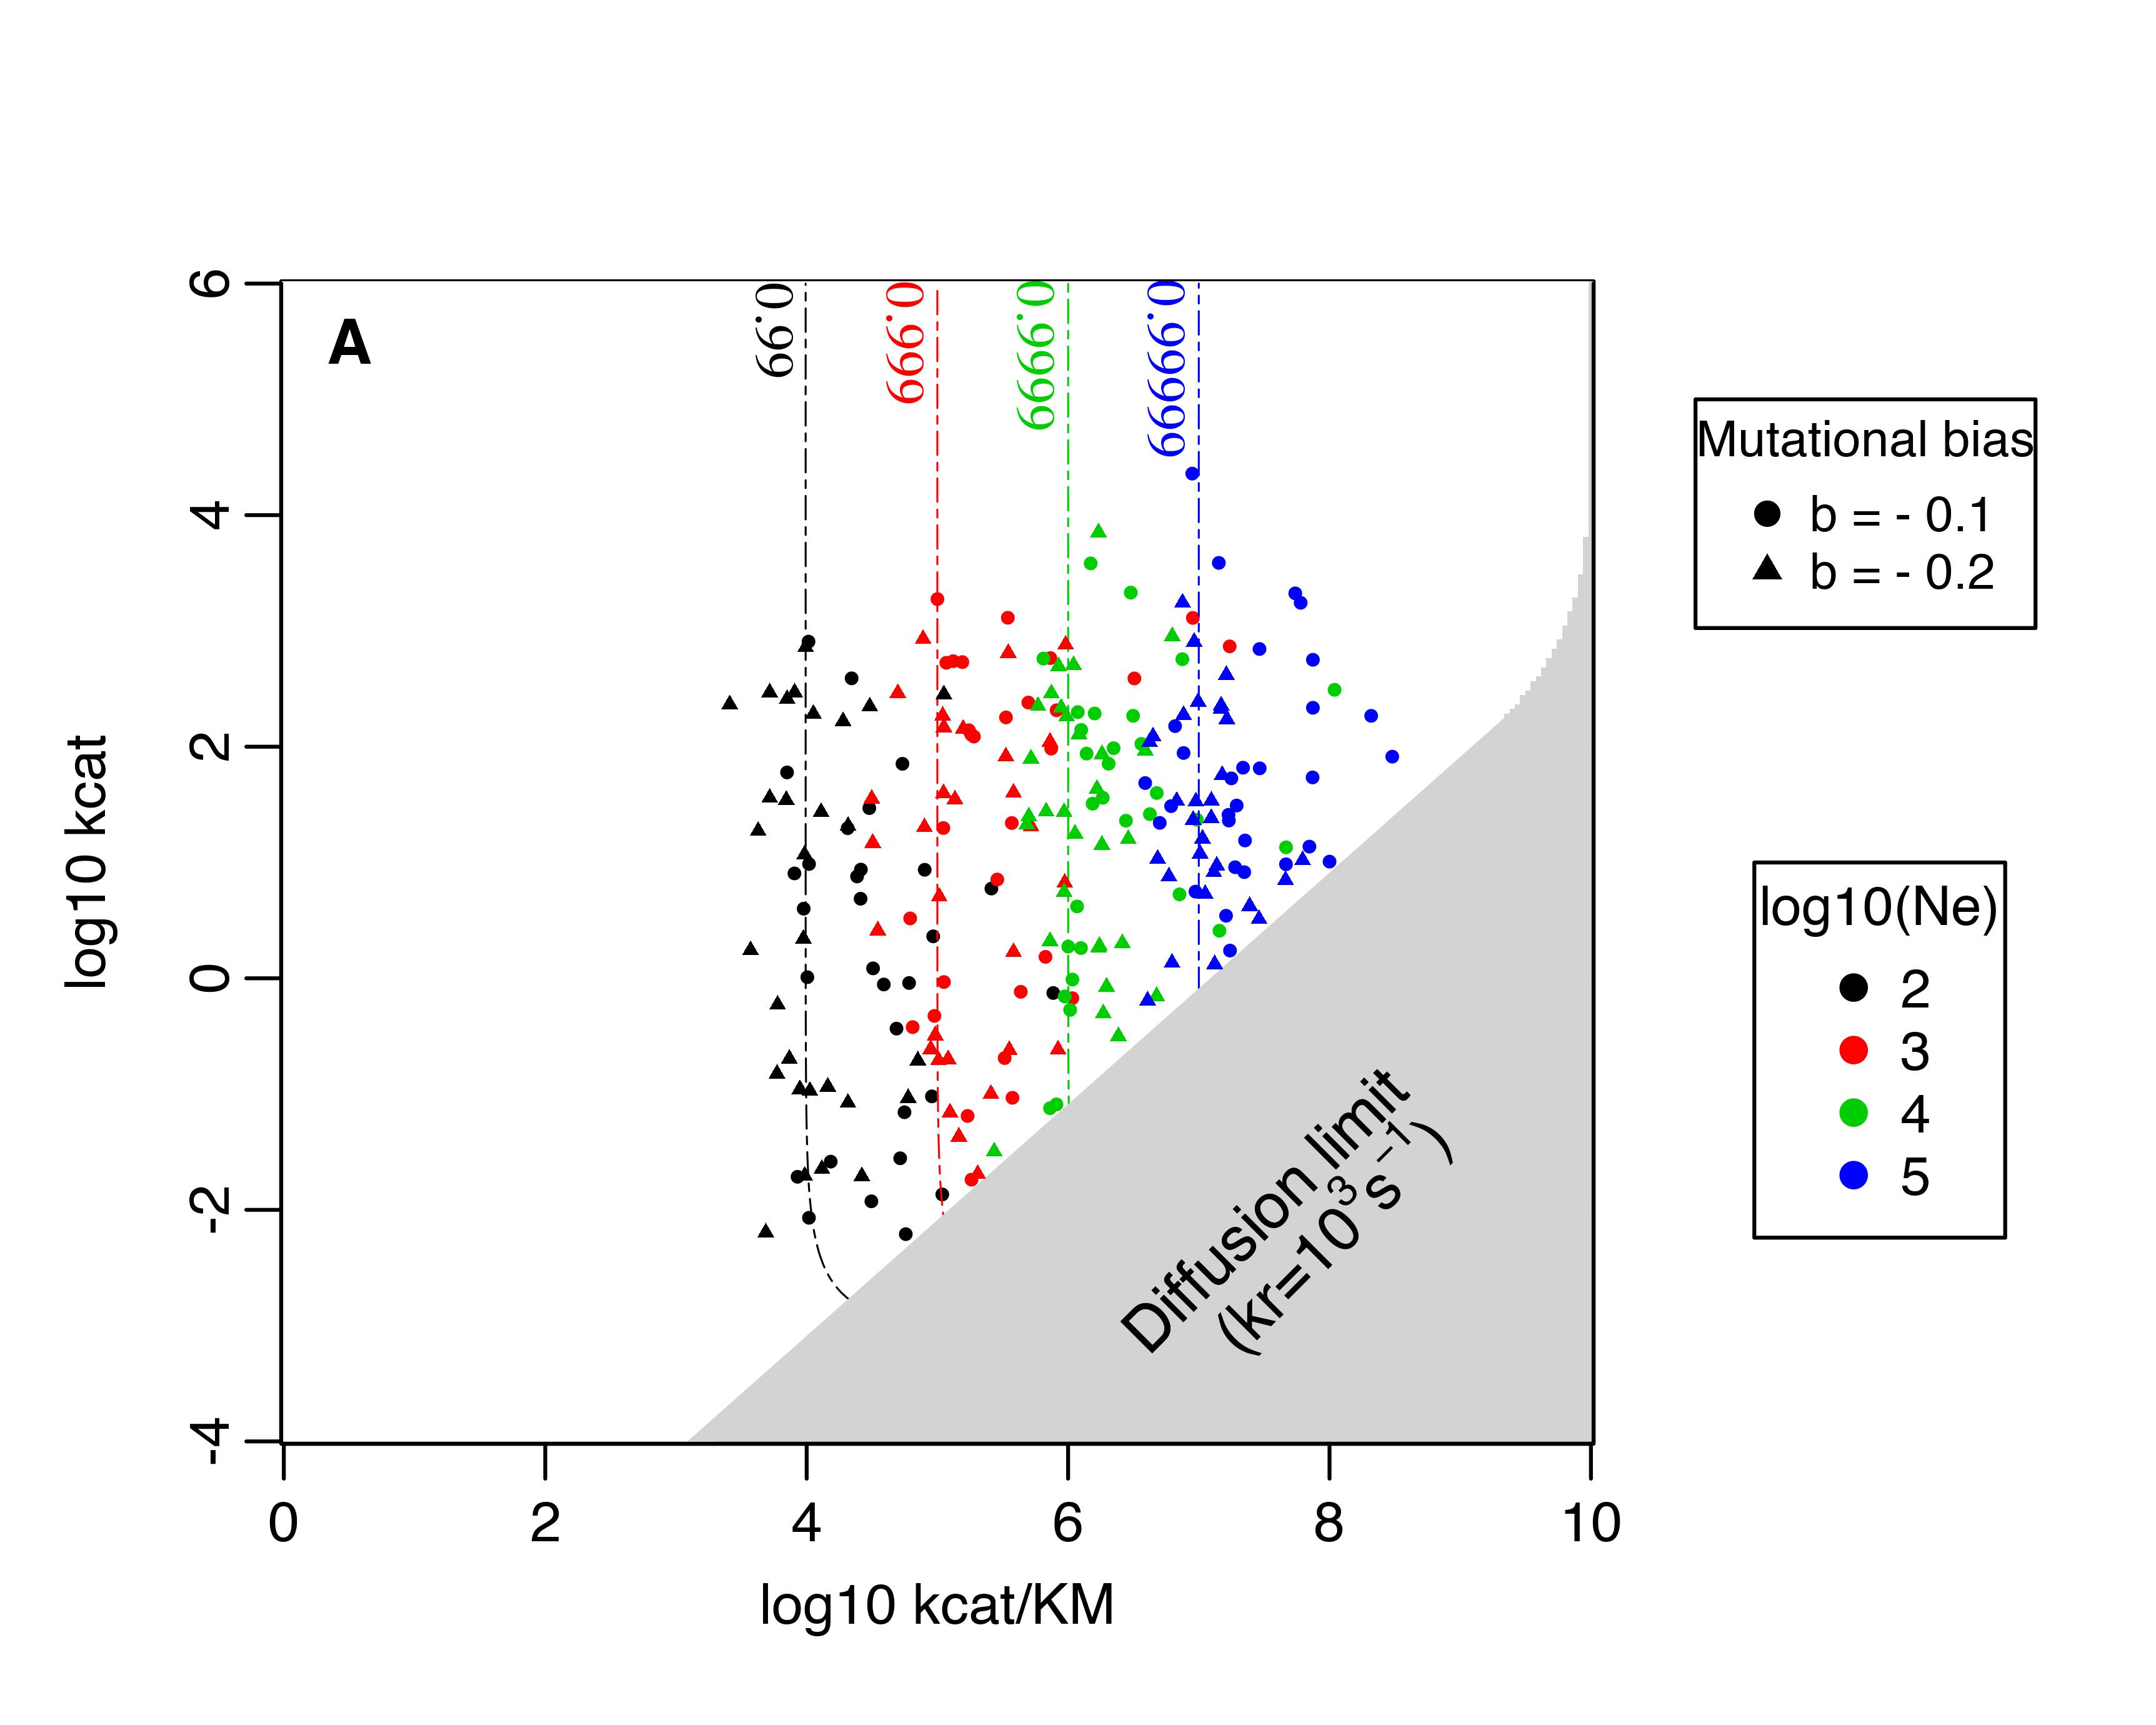
\includegraphics[scale=0.65,trim=0.25cm 0cm 0.5cm 1.5cm,clip]{pics/Enzymes/2DFitLandscape_Evo_Results_lowF_withbias_Def.jpeg} 
%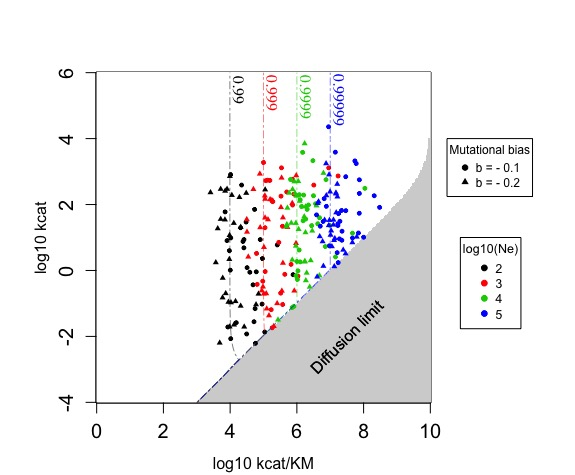
\includegraphics[scale=0.45]{Figures/2DFitLandscape_Evo_Results.jpeg}
%\includegraphics[scale=0.64,trim=0cm 0cm 3cm 1.5cm,clip]{Figures/.jpeg}
\end{minipage} \hspace{0.5cm}\hfill
\begin{minipage}[c]{0.46\linewidth}
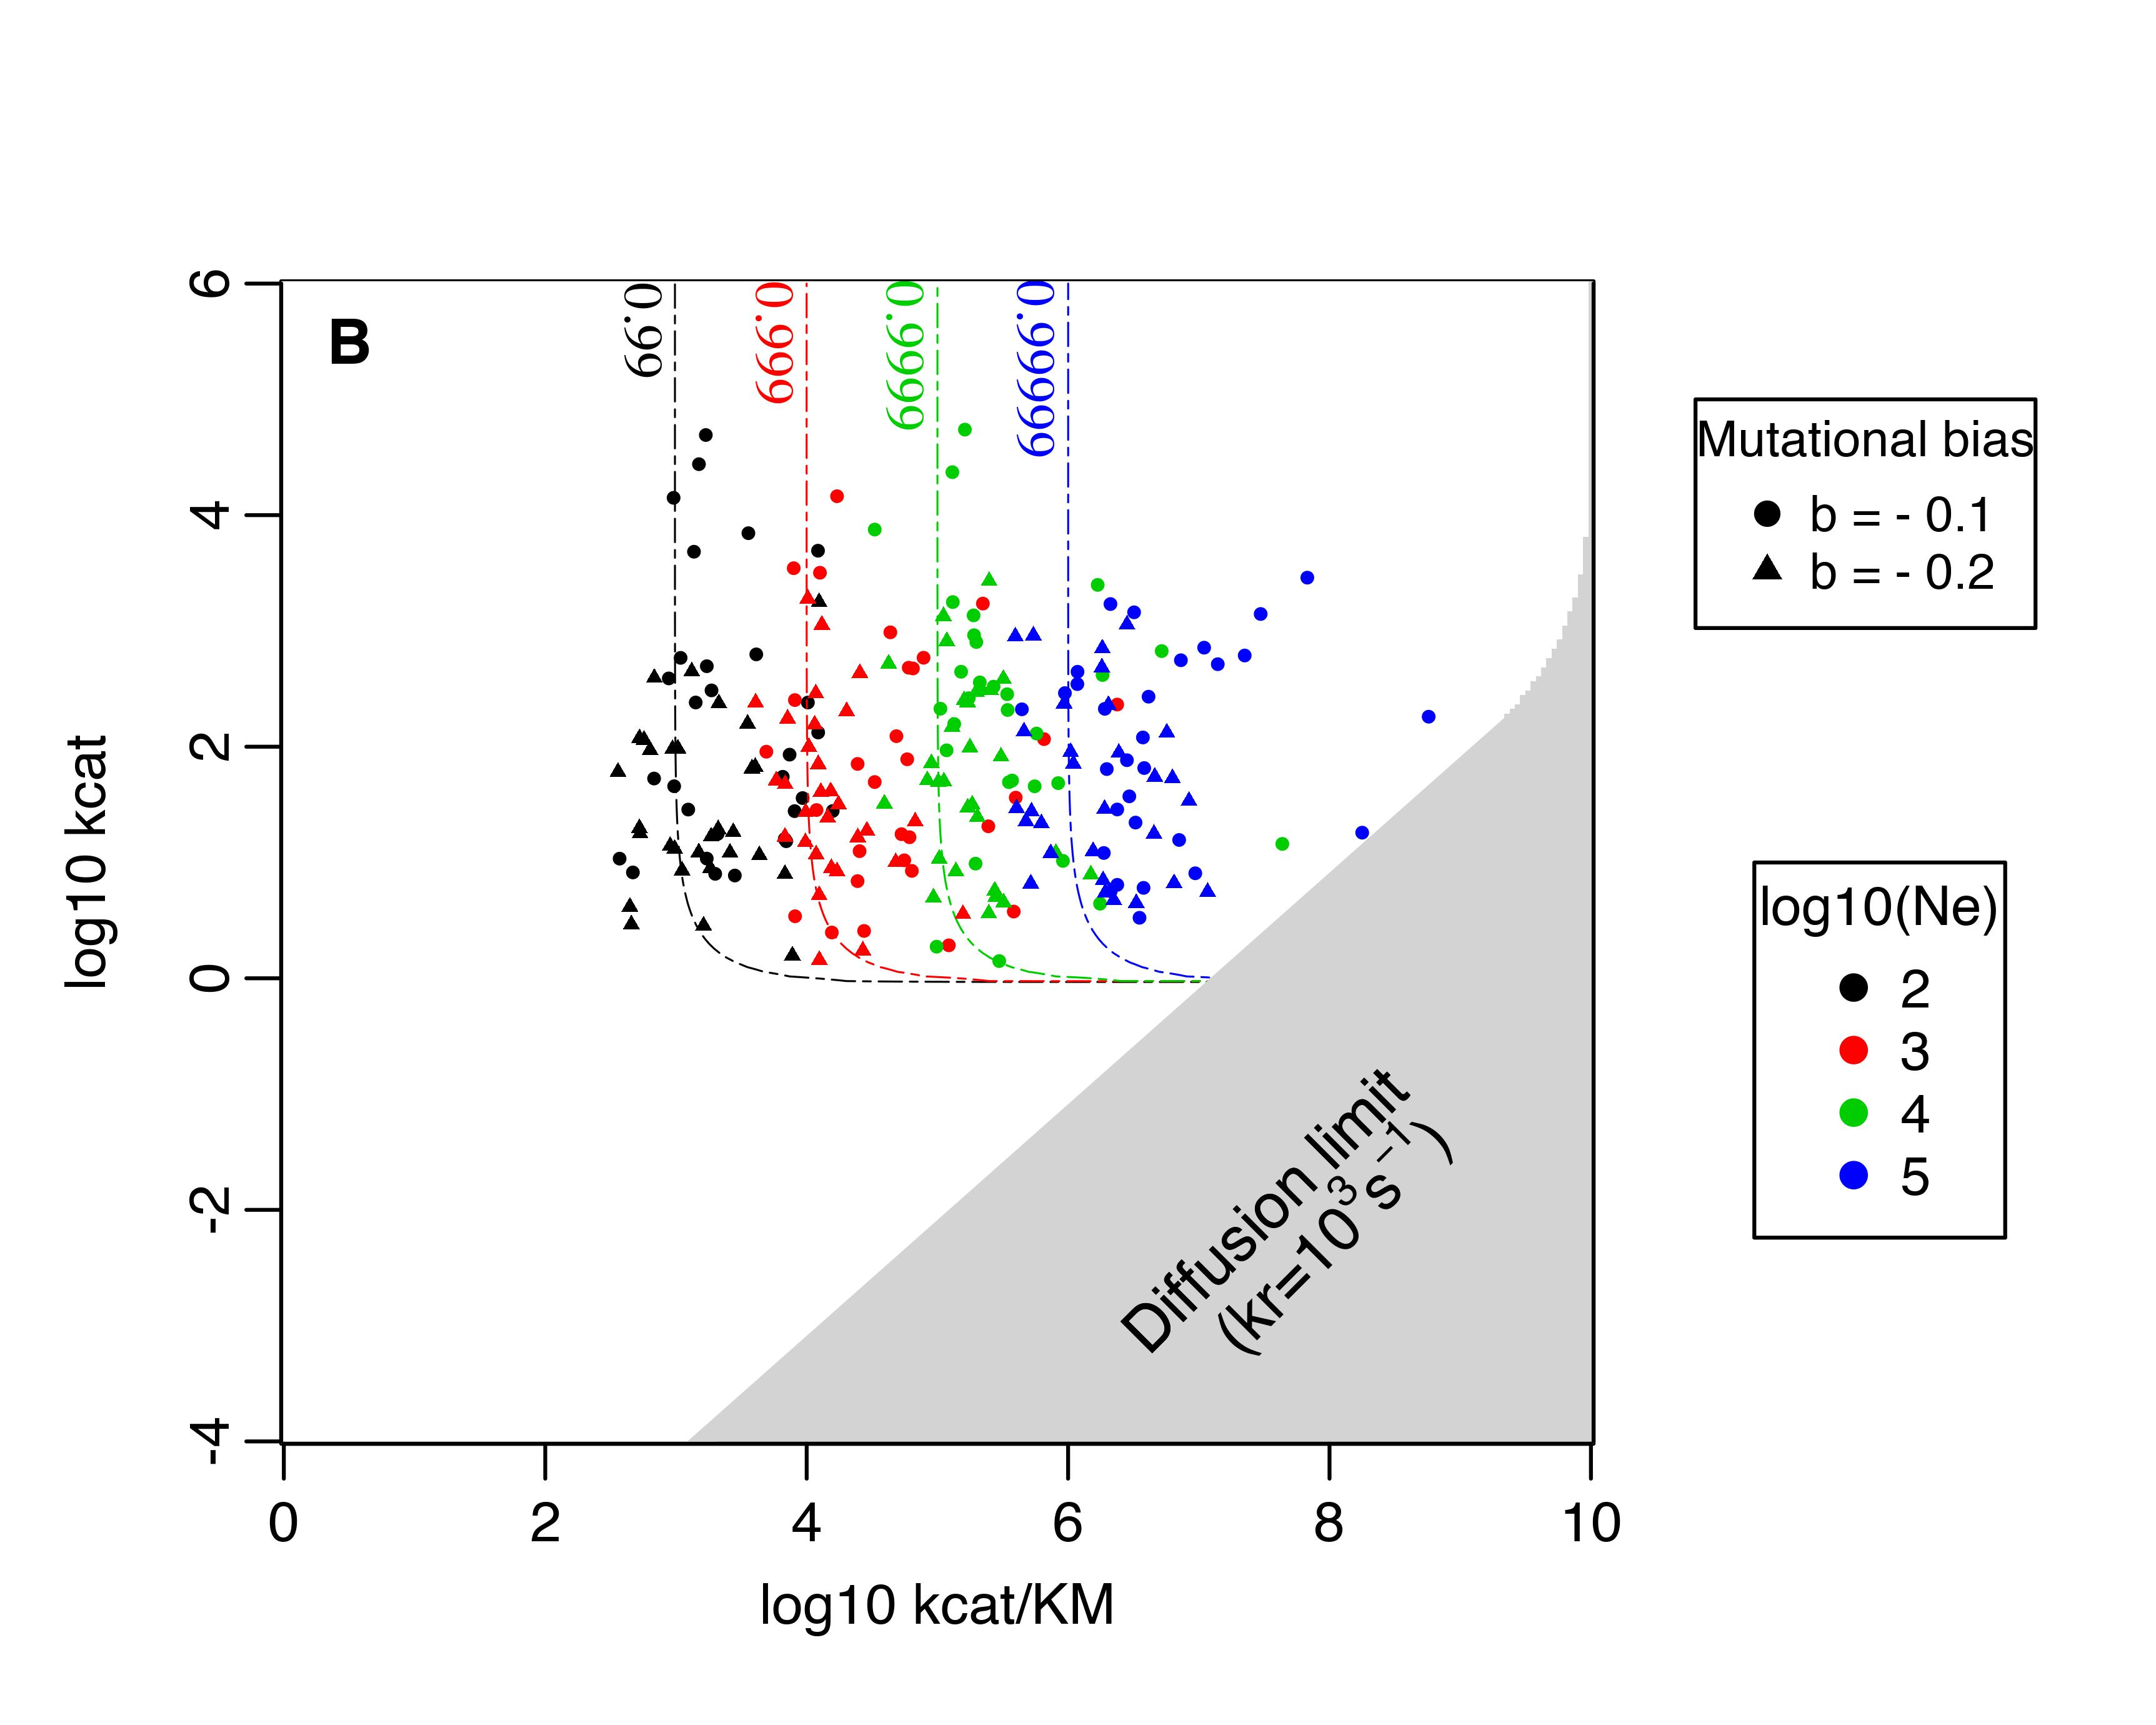
\includegraphics[scale=0.65,trim=0cm 0cm 3.5cm 1.5cm,clip]{pics/Enzymes/2DFitLandscape_Evo_Results_highF_withbias_Def.jpeg} 
\end{minipage}
%\vspace{0.5cm}
\caption{Population genetic simulations predict that enzymes should reach a predictable set of features when mutation biases towards lower efficiencies are considered (see SM  fig. S17 for the case of an absence of bias). Indeed, the mutation selection drift equilibrium establishes close to an isocline indicative of effective selection that depends on the effective population size $N_e$. The cases considered here are that of a transporter with a low flux at saturation and high affinity (A; $V_{Tm}=1\mu Ms^{-1}$ and $K_T=10\mu M$) and one with a high flux at saturation but low affinity (B; $V_{Tm}=1mMs^{-1}$ and $K_T=100mM$) with effective population sizes ranging from $10^2$ to $10^5$ (different colors) and two strengths of the mutational bias (the absence of mutational bias was also considered, see SM). Each of 30 independent simulations for each scenario is represented a dot in the ``empirical" parameter space ($k_\text{cat}, \;k_\text{cat}/K_M$), but only $k_\text{cat}$ and $k_f$ were susceptible to evolve. $k_r$ is set to $10^3s^{-1}$ such that the grey part of the parameter space is inaccessible to enzymes that would otherwise exceed the diffusion limit. 
}
\label{figure2D_Evolutionary_results}
\end{figure*}

How much variance in evolutionary outcomes these differences in fitness landscapes may explain is contingent on the interplay between selection, mutation and drift. Small differences in an isocline position should indeed be of little importance if populations perform random walks on the fitness plateau, for instance. To approach how populations evolve on our mathematically derived fitness landscapes, we built a simple population genetics model in which absolute fitness is directly proportional to the flux arising from the first enzyme at steady-state -- which itself equals the net inward flux of nutrients. Two different levels of metabolic demands were considered, corresponding to parameter values of amino acids/nucleosides and sugar transporters (panels (A) and (I) in SM Fig. S3). In this instance of the model, only $k_\text{cat}$ and $k_f$ were susceptible to evolve through mutations. Mutational effects on $\log_{10}k_{cat}$ and $\log_{10}k_f$ were drawn from independent normal distributions with mean $b \leq 0$, and the absolute value of $b$ setting the intensity of a mutational bias towards less efficient parameter values, as has been widely documented in many contexts \citep{EyreWalker07,Serohijos12,Heckmann18}. The standard deviation of the distribution of mutational effects equals $0.3$ such that most mutations explore the neighbouring parameter space,  seldom changing a parameter by more than one order of magnitude (one $\log_{10}$ unit) in compliance with empirical estimates \citep{Carlin16}. Since the relation between kinetic parameters may be constrained -- \textit{e.g.} due to shared properties of the energy profile of a reaction -- we tested the influence of negative and positive relationships using bivariate normal distributions, with three different values of $\rho$ (see Materials and Methods for details). 

In the absence of mutational bias ($b=0$), simulated enzymes spread over the fitness plateau, as expected (Fig.~S16-A for low flux, Fig.~S17A otherwise). The onset of the plateau depends on the strength of drift and hence derive from the effective population size $N_e$, following the classical expectation that selection becomes inefficient when $N_e \times s < 1$ \citep{Wright31,Kimura68}. Introducing a mutational bias that makes enzyme kinetics less efficient on average has a strong effect on both $k_\text{cat}$ and $k_f$, preventing simulated enzymes from improving far above the drift barrier (FIG.~\ref{figure2D_Evolutionary_results}-A for low flux, FIG.~\ref{figure2D_Evolutionary_results}-B otherwise). 
Even weak biases ($b=-0.1$) lead to enzymes evolving in the vicinity of the isocline where $N_e \times s \approx 1$. Increasing the strength of this bias to $0.2$ only slightly decreases the population variance around this expectation. Finally, mutational correlations do not impact much the distribution of evolutionary outcomes (SM Fig. S18).

Our results suggest a strong effect of the effective population size on enzyme evolution, such that species with $N_e$ above $10^5$ \citep[most unicellular organisms]{Bobay18} should express extremely efficient enzymes. This appears to not be the case, as for instance Eukaryotes and Prokaryotes display similar enzymes despite large differences in effective population sizes \citep{Bar-Even11}. As we will later discuss, this conundrum might resolve when considering the smaller size of organisms forming large populations, making them more sensitive to noise in gene expression and favouring higher concentrations. 
%It is thus possible that the role of genetic drift is not well captured by a model that considers small parts of a large system in isolation, or more generally that the link between fitness and flux is not as straightforward as we have assumed. 
Notwithstanding this issue, the prediction of enzymes evolving a predictable set of kinetic parameters strongly suggests that a large part of the broad variance in enzyme features is due to differences in the selective context experienced by each, thereupon requiring further investigation on the dependency of the position of the fitness plateau to parameters of our model.

\noindent \paragraph{The joint evolution of enzyme concentrations and kinetic parameters}

\begin{figure}[h!]
\centering
\begin{minipage}[c]{0.5\linewidth}
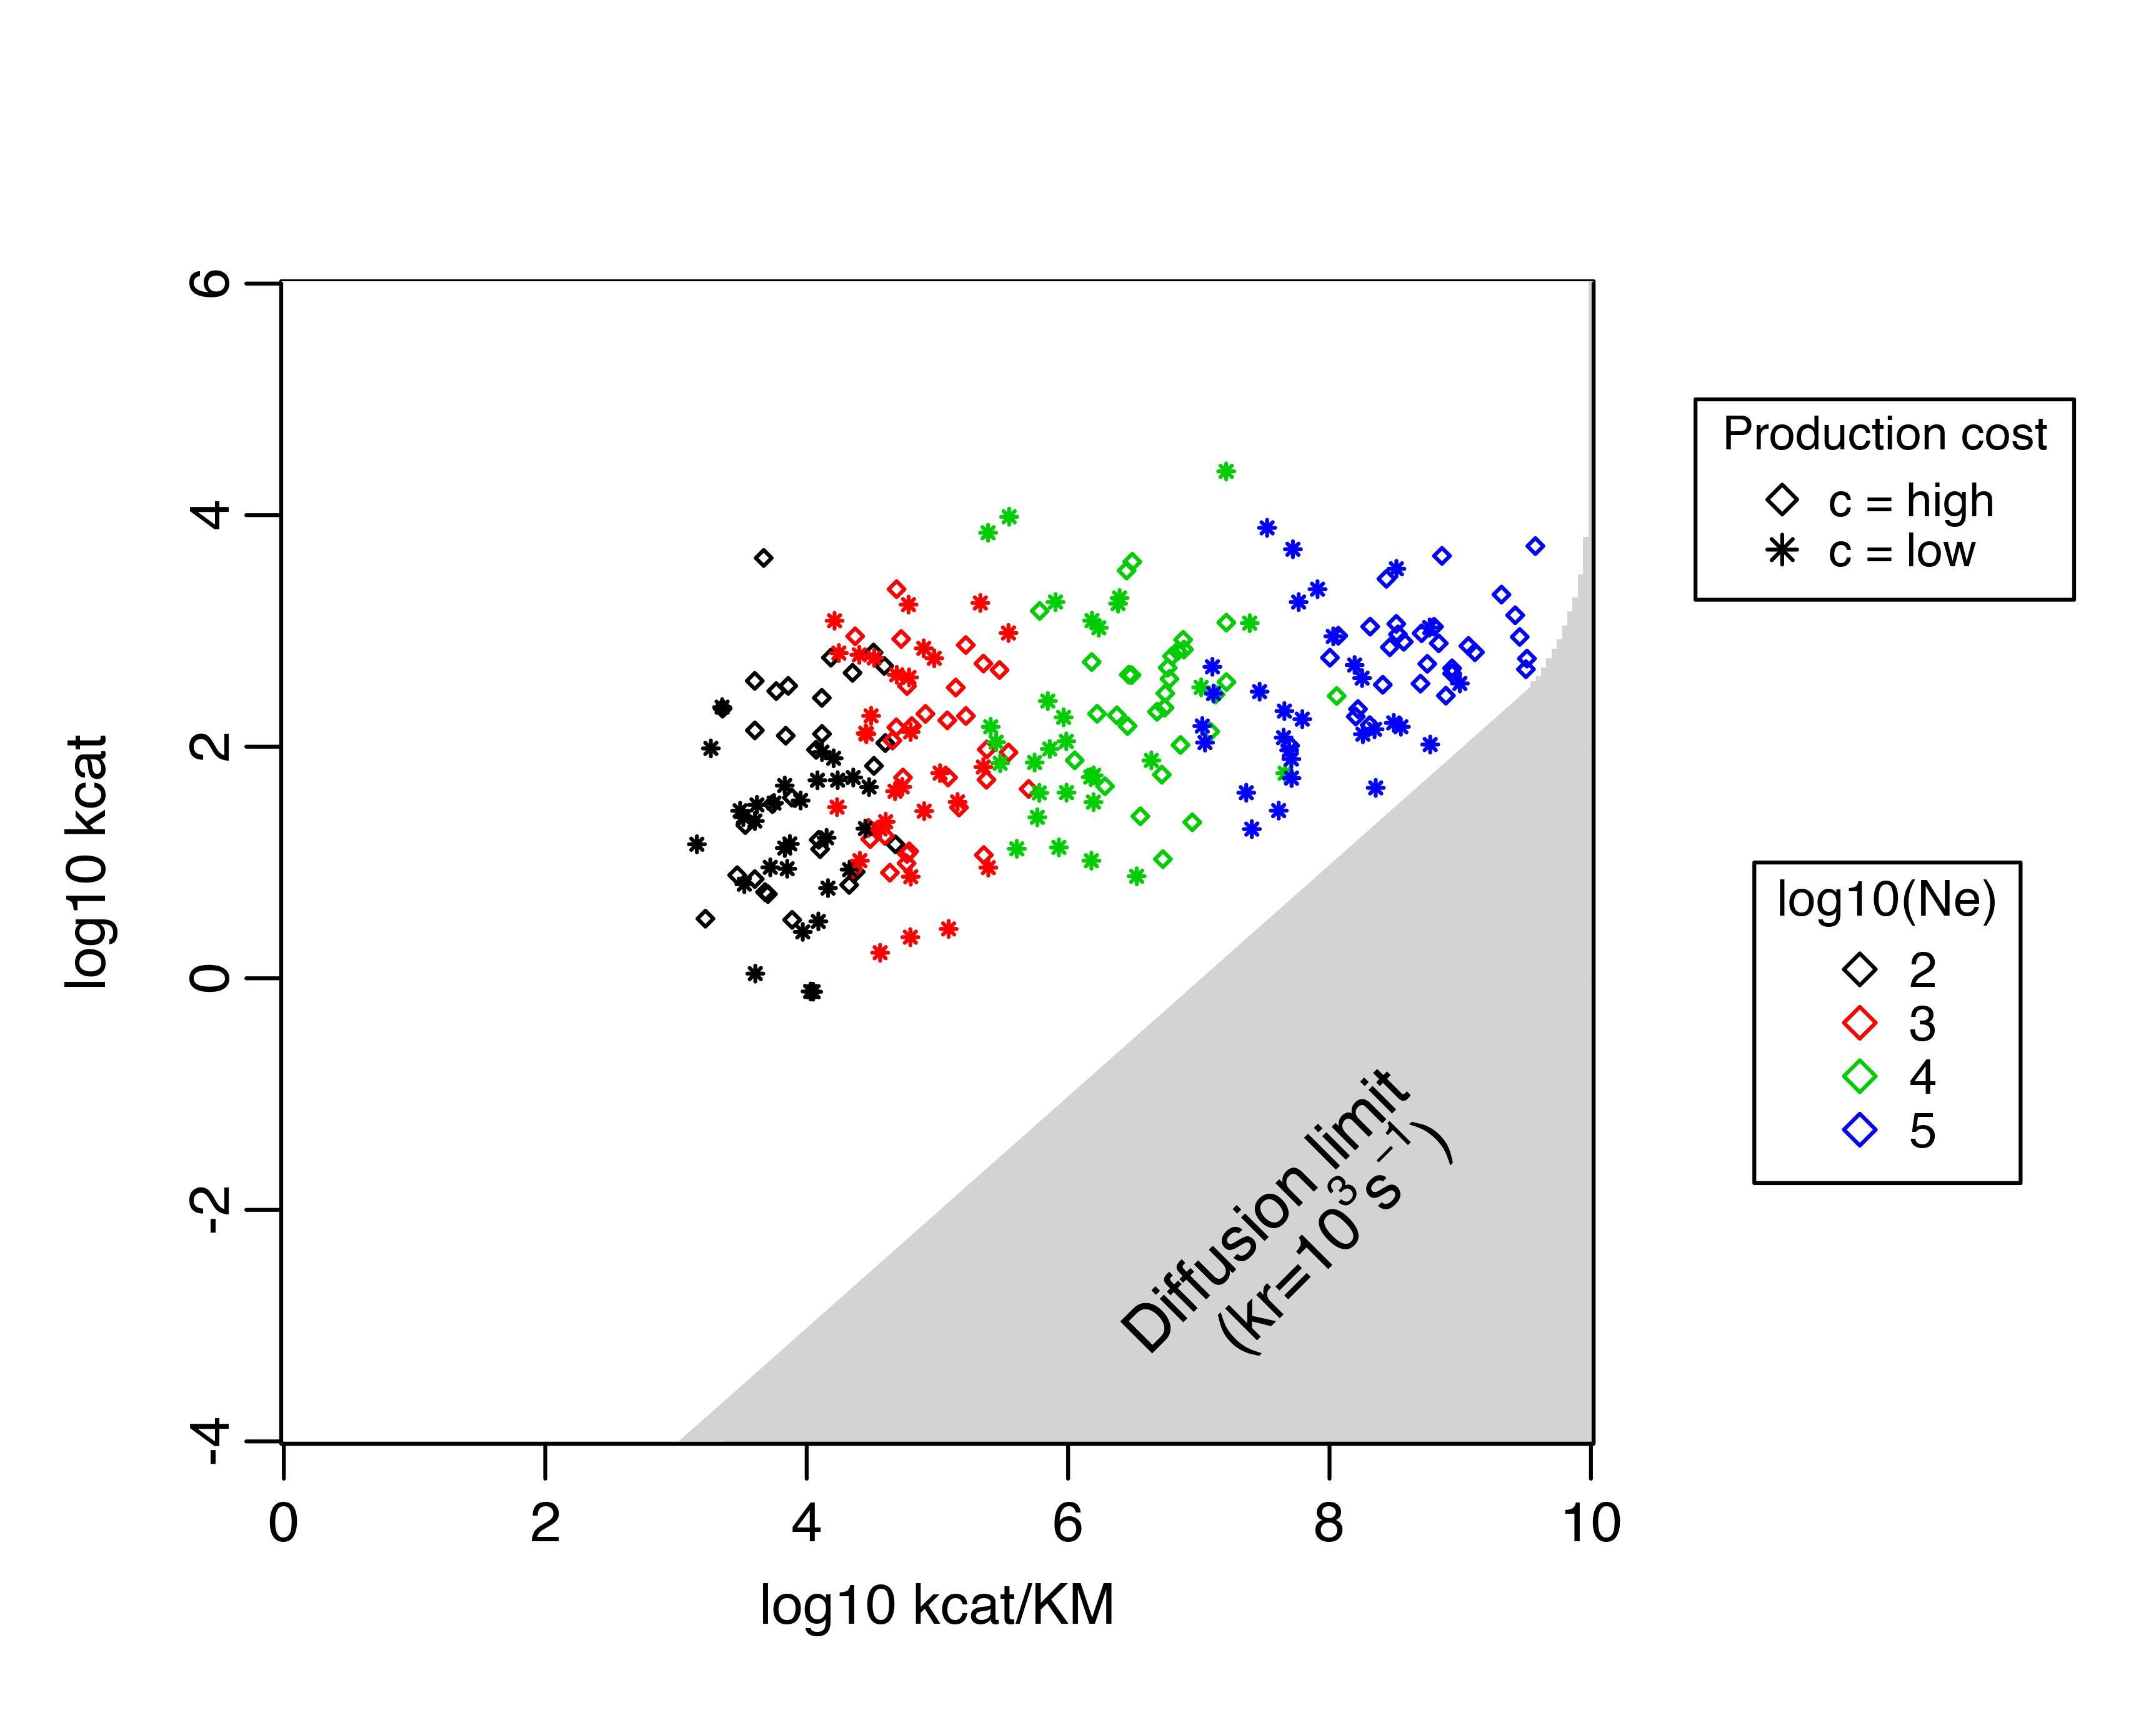
\includegraphics[scale=0.65,trim=0.25cm 0cm 0cm 0.75cm,clip]{pics/Enzymes/Evo_Results_CostCrow_PaperModM.jpeg}
\caption{Simulations of the joint evolution of en-}
\label{figure2D_Evolutionary_results_HF}
\end{minipage}
\hspace{0.5cm}\hfill
\begin{minipage}[c]{0.42\linewidth}
%\vspace{0.5cm}
\caption*{zyme concentration and kinetic parameters, with a twofold cost of enzyme overexpression (the direct metabolic cost and the indirect cost of cell packing). The case considered here is that of a transporter with a high flux at saturation and low affinity ($V_{Tm}=1 mMs^{-1}$ and $K_T=1mM$) under a high mutational bias on kinetic constants ($b=-0.2$). Two different costs of protein production $c$ are considered along with four effective population sizes ranging from $10^2$ to $10^5$. We ran 30 independent simulations for each scenario, each represented by a dot in the ``empirical" parameter space as described in fig.~\ref{figure2D_Evolutionary_results}.
}
\end{minipage}
\end{figure}

Hitherto, we have considered enzymes to be highly concentrated, an assumption that we now relax since it is an important component of the presumed kinetic activity \citep{Koshland02}. Predictably, increasing the concentration of the first or second enzyme in a pathway releases the selection on their kinetic parameters \citep{Noor16}, producing larger fitness plateaus as an enzyme concentration increases (see SM - Figs S12-B and S13-B for this influence in different contexts). Due to the compensatory effects between concentration and activity, we anticipate that the joint evolutionary dynamics of the concentration and kinetic parameters should yield a negative correlation between them, as reported by \citet{Davidi16,Davidi18}. 

Despite their common role on reaction efficiency, enzyme concentration expectedly responds to very different selection pressures than kinetic parameters, as increased gene expression levels come with costs \citep{Wagner05,Lang09,ScottM10,Noor16,Kafri16}. Indeed, producing extra proteins requires both energy and matter \citep{Novick57,Stoebel08,Wagner05,Lynch15} and may impede the efficiency of physical processes that rely on an optimal intermediate content \citep{Dong95,Dill11,Andrews20}. We designed a new instance of our population genetics model to study the tangled evolution of kinetic constants and enzyme concentration, introducing two of these costs: (1) the cost of producing proteins $c$, considered to be proportional to concentration \citep{Wagner05,Chou14,Lynch15}, and (2) the exponential cost of an increase in macromolecular crowding, which hinders diffusion and thus slows down reactions \citep{Dill11,Schavemaker18,Andrews20} 
% when cellular concentrations go beyond a threshold $[Proteome] \approx 3-4 mM$ 
(see SM Fig. S15 for the resulting fitness landscapes of enzyme concentration).

The two types of costs result in a different shape of the fitness landscape, with the noticeable difference that evolutionarily expected concentration depends on $N_e$ when the cost of production is considered (SM - Fig. S19) but not with crowding effects (SM - Fig. S20). With a combination of the two costs, enzyme concentrations decrease with $N_e$ and production costs, resulting in the evolution of higher kinetic constants (FIG. \ref{figure2D_Evolutionary_results_HF}). This is because at higher effective sizes, direct costs of protein production are large enough to incur effective selection for lower protein expression. This is no longer the case when $N_e$ decreases, such that the major force driving the optimization of enzyme concentration becomes that opposing macromolecular crowding, which is less sensitive to $N_e$ (as shown in Fig. S19 in SM). The balance between these two selective forces, and the dependency to $N_e$, obviously depend on the relative importance of these costs (SM - Fig. S20), itself depending on many parameters (protein length, molecular weight, etc.) that should only make enzymes marginally different within a given species (when their activity evolves on similar fitness landscapes).
%The balance between these two fitness costs and their screening by Natural Selection is obviously sensitive to the precise value of the cost of production (see SM Figure S20 also), but overall, they can only explain marginally differences between enzymes of a given species. Even more striking is the fact that under the two assumptions made, big enough $N_e$s should lead to even more efficient enzymes, calling for the need of even more mechanistic models of fitness as indicated in the discussion. Noticeably, because the mutational landscape of gene expression is more balanced than that of kinetic parameters, playing on concentrations proved to evolve quicker and approach more readily the fitness plateau of activity. Only then, the fine tuning of enzymes occurs through the improvement of kinetic parameters.

\subsubsection{Discussion\label{sec:Discussion}}

Most enzymes have been considered to be only moderately efficient \citep{Bar-Even11}, if not sloppy \citep{Bar-Even15}. This claim was put into perspective by \citet{Newton18} who argued that the link between fitness and enzyme efficiencies is complex and may be partly enzyme dependent, such that all enzymes may not evolve on a common fitness landscape. Through this work, we have developed a model where enzyme efficiencies are mechanistically linked to fitness through the impact of nutrient gradients on the production of metabolites. Our results emphasize that an enzyme's fitness landscape -- and the resulting mutation-selection-drift balance -- may indeed be largely context dependent, possibly explaining a large part of the extreme observed variance in enzyme features.

At first sight, all enzymes evolve on fitness landscapes that have the same general shape, with a fitness plateau surrounded by a steep slope. While this shape is usual in models of enzyme evolution \citep{Hartl85,Kaltenbach14,Yi19}, in our model the landscape is drawn in the parameter space formed by the two forward kinetic parameters $k_\text{cat}$ and $k_f$, instead of a composite ``efficiency'' whose relevance is questionable \citep{Eisenthal07,Koshland02}. Our model allows to predict the precise position of the fitness plateau in various contexts, showing that model parameters may have a selective impact on $k_f$, $k_\text{cat}$, or both, thereby confirming the relevance of considering their distinct evolutionary dynamics. 

We have shown that the exact position of the plateau is important through a population genetics model including mutational biases that produce less efficient enzymes at a slightly higher frequency. Despite their small effect, these biases are sufficient to have a significant impact on the evolutionary dynamics occurring on the fitness plateau, preventing enzymes to explore the parameter space far away from an isocline whose precise value can be predicted. Because the mutation-selection-drift balance occupies a narrow part of the landscape, this makes the evolution of an enzyme, in principle, highly predictable. Likewise, we anticipate that differences between enzymes should largely be explained by differences in the shapes of their individual fitness landscapes. 

Overall, the selective pressure acting on an enzyme results from an interplay between several biochemical factors. We have effectively found that the shape of the fitness landscape is first governed by features of the transporter initiating a pathway, especially the maximum flux they can sustain. Using parameters that correspond to empirical estimates for sugars and amino acids/nucleosides, we have found that enzymes contributing to subsequent metabolic pathways should be different, with those in the ``sugars" pathway being selected for faster kinetics.

While sharing a common transporter, enzymes along a pathway are also subject to a variety of local chemical contexts, making each evolve on its own unique fitness landscape. This could explain, at least in part, the large within-pathway variance of enzyme kinetic parameters. Physical constraints may for instance act differentially on different enzymes, as exemplified by the intrinsic reversibility of a reaction that fuels the selective pressure towards higher efficiency in downstream enzymes. This may contribute to explain the high efficiency of a few enzymes like TIM %, and thereby why there exists some ``equilibrium enzymes" pushing reactions close to their chemical equilibrium 
\citep{Williamson67,Davidi18}.

One way to compensate for low kinetic constants is to enhance the level of expression of an enzyme, as confirmed by our model -- concentration indeed has a strong influence on the fitness landscape of $k_f$ and $k_\text{cat}$. Nonetheless, concentration and kinetic parameters face very distinct selection regimes: while the latter are both under directional selection, vanishing at high efficiencies, concentration is under stabilizing selection -- owing to a combination between its positive impact on the flux and the adverse costs to high expression -- as already pinpointed by \citet{Chou14}. Their joint evolution is complex because the position of the concentration optimum depends on an enzyme's kinetic constants, whose fitness landscape itself depends on concentration. This results in a slightly increased variance in enzyme efficiencies compared to simulations with fixed concentrations, along with a complex relationship with genetic drift, because small populations tend to tolerate higher enzyme concentrations and, therefore, evolve less efficient enzymes.

It should be noted that our model does not consider another selection pressure on enzyme concentrations that arises from noise in gene expression, as argued by \citet{Wang11}. Indeed, low expression results in detrimental noise that should be avoided by pushing enzyme concentrations towards higher values in small organisms like Prokaryotes (see SM section Text S6 for an estimate of this effect). This could result in a different relationship between $N_e$ and enzyme efficiencies than considered here, possibly explaining the confusing observation that species with larger populations (and smaller sizes) do not express markedly more efficient catalysts. Furthermore, an enzyme's effective concentration can also increase through compartmentalization \citep{Ovadi04,Diekmann13,Cornejo14} and substrate channeling \citep{Welch94,Huang01,Sweetlove18}, within the limits imposed by noise, and modify the selective pressure acting on kinetic parameters.

This illustrates that rather than making precise predictions, our study aims at making the strong claim that selection acting on enzyme features is important for their diversity, possibly largely overcoming the diversity arising from neutral processes. If this is indeed the case, trends in enzyme evolution can be predicted -- as it was shown empirically in the context of antibiotic resistance \citep{Walkiewicz12} -- and further improvements of this model should allow one to predict the expected features of individual enzymes. Such improvements are made easier by the use of a mechanistic framework, where fitness arises as enzymatic efficiency helps ingesting nutrients and win the competition for resources. This framework could even be enriched by other dimensions relevant to the genotype-phenotype-fitness map \citep{Bershtein17,Echave19,Kinsler20}. 

Unfortunately, mechanistic does not mean free of a definition of fitness, as we have here assumed that the latter is proportional to metabolic flux, hence considering each flux in isolation. Fitness instead results from a wide range of metabolic pathways that combine together and should all be competitive to certain degrees. How global epistasis builds up \citep{Weinreich13,Otwinowski18,Reddy20}, and genetic drift acts in this context, is far from obvious \citep{Iwasa04,Weinreich05,Weissman09}. But this should not impact much how enzymes evolve in old, overall efficient pathways, as any impediment in efficiency should have a relatively independent effect on fitness in this context, as captured by our model. Understanding these complex interactions between pathways would nevertheless be crucial to understand how metabolic pathways arose and improved, likely from a highly inefficient state during early steps in the evolution of life on Earth \citep{Kacser84,Schmidt03,Heckmann18}.


%While our focus was not on the evolution of interactions within and between pathways and high-order epistasis, the results of the model considering the evolution of neighbouring enzymes in a pathway suggest that any inefficient enzyme in the pathway should make virtually all other enzymes evolve on 

%Pour moi, il faudrait focaliser à ce stade sur  ce qu'il manque dans le modèle (les questions d'interactions en grande dimension), puis dire dans quel cadre le modèle est déjà crucial. Cela nécessite de couper le dernier paragraphe, ce qui ne te plait pas trop, du coup j'attends ton retour là-dessus. Pour la concentration, il me semble qu'avancer des choses est quand même très hasardeux vu les phénomènes qui peuvent biaiser l'interprétation, j'ai l'impression que cela peut plutôt faire partie de cette idée d'épistasie, en disant que pour comprendre l'évolution de ce genre de systèmes il faut en étudier conjointement les composants. Ce qui me gêne si on met l'évolution des transporteurs plus ahut, c'est que cela conduit à revenir à plusieurs reprises sur l'idée d'épistasie/interactions.

%, addressing the role of concentration on current enzyme features, empirically, should be much more straighforward. Indeed, as enzyme concentrations seemingly mutates more frequently, its ...

%J'ai l'impression que c'est un peu casse-gueule parce que c'est ce qui est fait largement dans la théorie du contrôle du flux, dont on veut se démarquer. Je pense que c'est bien si à ce stade on se concentre vraimen sur l'aspect évolutif, sur lequel on a le plus de choses à dire je crois.



%In parallel, we have made the assumption that enzymes could readily escape the stability-activity trade-off. It is however still unclear whether this trade-off can preclude cells to reach optimalities for both these quantities, at least in some enzymes, because enzymes first need to fold correctly before accomplishing their task while folded protein without activity only fuels the protein burden. If stability has allowed to understand the evolution of many molecular processes (as summarized in the introduction), it has been shown that stability and activity may widely be involved in the selective presures acting at the molecular level \citep{Echave19}. This calls for the need to more mechanistic models linking genotypes to phenotypes and fitness \cite{Bershtein17}, that will on the one hand enable to grasp what truly shapes cellular efficiency as a whole and on the other hand help understand the reported patterns of molecular evolution acting on genomes.



%Plus trop convaincu par ce dernier paragraphe pour l'instant; j'ai l'impression que c'est une pierre pour construire un modèle d'évolution des voies enzymatiques y compris une fois qu'elles sont déjà présentes, mais qu'il faut évidemment introduire ces interactions, ce qui peut être fait à l'aide de ce modèle sans faire d'hypothèses invérifiables.

\subsubsection{Materials and Methods\label{sec:M&M}}

%%%\subsection{Validation of the analytical solutions and Raphson Newton approach}

%%%Both analytical solutions -- for (PD) and (FD) -- were tested and therefore validated with different sets of kinetic values for the enzymes (cf.table X1 in Appendix). The Raphson Newton algorithm implementation was also checked for the two enzymes model it was designed for, showing quick and accurate convergence towards solutions determined when Euler explicit method was used to simulate the reaction kinetics (cf.table X2 in Appendix).

%Détail intéressant mais dispensable vu le besoin impérieux de place: Furthermore, this selective pressure might also help explain the phenomenon of substrate channeling, which brings a hedge against competition by collocating reactions \citep{Rickey-Welch94,Sweetlove18}.

%ER A déplacer dans le MM

\noindent \paragraph{Quantifying the maximum size for cells using passive diffusion}

If a cell is to be viable, it has, at least, to uptake enough glucose to compensate for basal metabolism -- metabolism that allows to maintain the same cell size for non-actively growing cells \citep{Lynch15} -- leading to the following equation: $\phi_{PD}=C_M$, with $\phi_{PD}$ the uptake through passive diffusion and $C_M$ the basal metabolism demand. To calculate the maximum size a cell can reach using only passive diffusion, we relied on the formula $C_M=0.39V^{0.88} (10^9 ATP/hr)$ estimated in \citep{Lynch15}. We also assumed the cell to be of spherical shape, both concentrations -- inside and outside the cell -- to be constant with the cellular concentration staying so low that it can be overlooked, meaning that the uptake resulting from passive diffusion can merely be written as $\phi_{PD}=P.[S_{\text{out}}].\frac{SA_{\text{sphere}}}{V_{\text{sphere}}}$, where $SA_{\text{sphere}}$ and $V_{\text{sphere}}$ are the surface area and the volume of a sphere, and $P$ represents the cell permeability and was measured to $10^{-6}\mu m^{-1}$ \citep{Wood68} for glucose. Finally, we considered that each glucose yields 30 ATP molecules \citep{Rich03}. 

\noindent \paragraph{Flux sustained by the first enzyme}

When assessing the flux of product made by the first enzyme in a pathway, both (PD) and (FD) result in similar sets of equations; we focus on FD here (see Text S5 - Mathematical appendix in Supplementary material for a comparison with PD). FD typically relies on the specific binding of substrate molecules -- located outside the cell -- by transmembrane carrier proteins, followed by their translocation into the cytoplasm \citep{danielli1954,Wilbrandt61,Kotyk67,Bosdriesz18}. This specific process obeys Michaelis Menten-like kinetics when transport is assumed to be symmetric \citep{Kotyk67}, which can be modelled through Briggs-Haldane equations \citep{Briggs25,Haldane30,Stein86d}:

\small
\begin{equation}
\frac{d[S_\text{in}]}{dt}=V_{Tm}.\frac{[S_\text{out}]-[S_\text{in}]}{K_T+([S_\text{out}]+[S_\text{in}])+\alpha.\frac{[S_\text{out}][S_\text{in}]}{K_T}}
\end{equation}
\normalsize

with:
\small
\begin{equation*}
  \left\{
      \begin{aligned}
		&V_{Tm}\text{: the maximum rate of a given carrier protein;}\\
		&K_T\text{: a constant inversely proportional to the transpor-}\\
		&\text{  ter efficiency};\\
		&\alpha \text{ : the Kotyk interactive constant  capturing the dis-}\\
		&\text{  equilibrium between bound and free transporters.}
      \end{aligned}
    \right.
\end{equation*}
\normalsize

%Alongside the concentration gradient, the Kotyk interactive constant \cite{Kotyk67} also brings by something special because the efflux (\textit{i.e. outwards flow}) cannot be overlooked due to the emergence of saturation in the process \citep{Teusink98,Bosdriesz18}.
By construction, $\alpha$ cannot exceed 1 \cite{Kotyk67} and is close to this upper limit for sugars (\textit{e.g.} $\alpha=0.91$ for glucose \citep{Teusink98}, so we set $\alpha=1$ by default in this study, maximizing the effect of interaction).

A model including both FD and irreversible substrate conversion by an enzyme therefore corresponds to the following chemical equation:

\begin{equation}
\footnotesize
\schemestart
 S$_{out}$
 \arrow{<=>[$V_{Tm},K_T$][$\alpha$]}
 S$_{in}$ + E
 \arrow{<=>[$k_{f}$][$k_{r}$]}
 ES
 \arrow{->[*0$k_{\text{cat}}$]}
 E + P$$
\schemestop
\label{chemMMT1R}
\end{equation}

Using analytical tools (see \citet{Kuile94} and \citet{Bosdriesz18}, rederived in Supplementary material - Text S5 Mathematical appendix), the flux can be determined through the following set of equations:

\vspace{-0.25cm}
\small
\begin{align}
\strut
[ES]^*=\frac{k_f[S_{in}]^*}{k_{r}+k_{cat}+k_f[S_\text{in}]^*}.[E_{tot}]\\
v=\frac{d[P]}{dt}=k_{cat}[ES]^*
\end{align}

\normalsize
where:
\vspace{-0.25cm}

\small
\begin{align}
[S_\text{in}]^*=\frac{-b+\sqrt{b^2-4ac}}{2a}
\end{align}

\normalsize
with:
\small
\begin{equation}
  \left\{
      \begin{aligned}
        a&=k_f k_{cat}[E_{tot}](1+\frac{[S_{out}]}{K_T})+k_fV_{Tm}\\
		b&=k_f k_{cat}[E_{tot}]([S_{out}]+K_T)+(k_{cat}+k_r-k_f[S_{out}])V_{Tm}\\
		c&=-V_{Tm}[S_{out}](k_r+k_{cat})\\
      \end{aligned}
    \right.
\end{equation}

\normalsize
%\vspace{-0.5CM}
% Because of the Kotyk interaction constant -- set to $1$ -- the flux cannot reach the value of $V_{Tm}$, and rather stabilizes around an amount of product formed $\frac{d[P]}{dt}=0.9\mu M.s^{-1}$. In SM possibly

\noindent \paragraph{Multiple enzymes model}

In order to study the evolution of downstream enzymes, we considered an unbranched metabolic pathway in which the product formed by the first reaction serves as the substrate for a second reaction whose flux determines fitness. Theoretically, as there is nothing prohibiting increase in product concentrations -- for it is not considered reversible at this point -- any second enzyme should be able to sustain any metabolic demand. We penalized large increases in cellular concentrations through a degradation process of the product of the first reaction, occurring at rate $\eta_d$ ($\times$ this concentration). 
%This rate can result from outward diffusion, whose leak can be described with equations of passive diffusion (therefore, if we assume a low environment/outside concentration of the product, $\eta_d=P.SA/V$, with $P$, $SA$ and $V$ denoting similar quantities than in the (PD) case detailed in the first section of Materials and Methods). It may also arise as a by-product of non-specific or promiscuous activities where the product reacts with other metabolites or enzymes albeit with lower affinities, because such a reaction can be described through Michaelis Menten kinetics : assuming that $[P_1]<<K_M$ means that the amount of diverted - and therefore lost - product per unit time tends to $(k_{cat,ns}[E_{ns}]/K_{M,ns}) [P_1]$, where the parameters represent that associated with non specific kinetic activities. 
The chemical reactions occurring after uptake (Michaelis Menten part of Eq.\ref{chemMMT1R}) are described by the following equations:

\small
\begin{align}
\schemestart
 S$_{in}$ + E$_1$
 \arrow{<=>[$k_{f1}$][$k_{r1}$]}
 E$_1S$
 \arrow{->[*0$k_{\text{cat}1}$]}[0]
 E$_1$ + P$_{1}$
 \schemestop
 \label{chemMMT1R_deg}
 \end{align}
 \begin{align}
 \schemestart
 P$_{1}$ + E$_2$
 \arrow{<=>[$k_{f2}$][$k_{r2}$]}
 E$_2$P$_1$
 \arrow{->[*0$k_{\text{cat2}}$]}[0]
 E$_2$ + P$_{2}$
 \arrow(@c1--){->[*0$\eta_d$]}[-90]
 P$_{1out}$
\schemestop
\label{chemMMT2R_deg}
\end{align}

\normalsize
Such a system may reach a steady-state at which the cellular concentrations of the substrate $S_{in}$ and of the first product $P_1$ are constant. At this point, the net instantaneous uptake of substrate equals the instantaneous production of $P_1$ which, in turn, equals the sum of the instantaneous amount of degraded $P_1$ and the instantaneous production of $P_2$, according to the principle of mass conservation. It yields the following system of equations:

\footnotesize

\begin{equation}
		\begin{aligned}
V_{Tm}.&\frac{([S_{out}]-[S_{in}])}{K_T+([S_\text{out}]+[S_\text{in}])+\alpha.\frac{[S_\text{out}][S_\text{in}]}{K_T}}=V_{m1}.\frac{[S_{in}]}{K_{M1}+[S_{in}]}
		\end{aligned}
		\label{mathMMT1R_deg}
\end{equation}

\begin{equation}
\begin{aligned}
V_{m1}.&\frac{[S_{in}]}{K_{M1}+[S_{in}]}=V_{m2}.\frac{[P_1]}{K_{M2}+[P_1]}+\eta_d.[P_1]
		\end{aligned}
		\label{mathMMT2R_deg}
\end{equation}

\normalsize
\noindent where appear the traditional Michaelis-Menten kinetic parameters for the (i$^{eth}$) reaction:

\small
\begin{equation*}
  \left\{
      \begin{aligned}
		&V_{m_i}=k_{cat_i}[E_{tot_i}]\\
		&K_{M_i}=\frac{k_{r_i}+k_{cat_{i}}}{k_{f_{i}}}
      \end{aligned}
    \right.
\end{equation*}

\normalsize
To test the potential influence of toxicity, we defined the absolute fitness as a function of both the flux and a toxicity factor whose influence is represented through a sigmoid function and reflects the non-linearity nature of toxic effects \citep{Clark91,Wright10}: $f=\phi(1-\frac{[P]}{[P]+T})$

In an independent section, we also introduced reversibility through the modification of equation (\ref{chemMMT1R_deg}), which becomes:

\small
\begin{align}
\schemestart
 S$_{in}$ + E$_1$
 \arrow{<=>[$k_{f1}$][$k_{r1}$]}
 E$_1S$
 \arrow{<=>[*0$k_{\text{cat}1}$][$k_{inh1}$]}[0]
 E$_1$ + P$_{1}$
 \schemestop
 \label{chemMMT1R_degrev}
 \end{align}
 
\normalsize
Such a phenomenon is described by the more general form of Haldane equation \citep{Haldane30,Cornish-Bowden79a}, which changes the contribution of the first reaction ($V_{m1}.\frac{[S_{in}]}{K_{M1}+[S_{in}]}$) in both equations (\ref{mathMMT1R_deg}) and (\ref{mathMMT2R_deg}) to:

\footnotesize
\begin{equation*}
		\begin{aligned}
		V_{m1^{+}}.&\frac{[S_{in}]}{K_{M1^{+}}+[S_{in}]+K_I [P_1]}-V_{m1^{-}}.&\frac{[P_1]}{K_{M1^{-}}+[P_1]+[S_{in}]/K_I}
		\end{aligned}
		\label{mathMMT1R_rev}
\end{equation*}
\normalsize
with $V_{m1^{+}}$ and $K_{M1^{+}}$ respectively correponding to the previous $V_{m1}$ and $K_{M1}$, while:

\small
\begin{equation*}
  \left\{
      \begin{aligned}
		&V_{m1^{-}}=k_{r1}[E_{tot1}]\\
		&K_I=k_{inh1}/k_{f1}\\
		&K_{M1^{-}}=K_{M1^{+}}/K_I
      \end{aligned}
    \right.
\end{equation*}

\normalsize
To solve these systems %, which are not easily tractable analytically -- for they rely on cubic equations -- 
we implemented the Newton method \citep{Atkinson89} aiming to find $[S_{in}]^*$ and $[P_1]^*$. We ran the algorithm starting from very low values of concentration (both set to $10^{-20}M$) to determine numerically the equilibrium without facing convergence problems. The final flux can then be determined through the ``production'' part of equation (\ref{mathMMT2R_deg}), \textit{i.e.} $V_{m2}.\frac{[P_1]}{K_{M2}+[P_1]}$.


\noindent \paragraph{Validation of the method and computing of the fitness landscapes}

To validate the approach, we compared equilibrium results obtained with Raphson-Newton algorithm to those obtained when simulating the process with Euler explicit schemes for a set of (3x3) kinetic values -- $k_\text{cat}$ and $k_f$ -- encompassing three orders of magnitude (see SM - Section Text 5 for further details).

We then drew fitness landscapes after determining the flux -- assumed to be to be linearly related to fitness -- achieved for enzyme kinetic parameters $k_\text{cat}$ and $k_f$ varying by 10 orders of magnitude, setting $k_r$ to $10^3 s^{-1}$ -- within the range found for several enzymes \citep{Klipp94,Knowles77} -- unless stated otherwise. Except in the section dedicated to the influence of enzyme concentration, we set the enzyme concentration such that $[E_{tot}]=1mM$, lying nearby the highest observed values \citep{Albe90,Noor16}. Other parameters are detailed on a case-by-case basis as they may change depending on the goal of each section. To compare with the data and visualize results in the experimenter's parameter space, we also determined the flux and plotted simulation results using $k_\text{cat}$ and $\frac{k_\text{cat}}{K_M}$, also making them vary by 10 orders of magnitude. We divided the parameter space in 100 log-equidistant values (250 for representations with $k_{cat}/K_M$ to obtain a cleaner demarcation for the diffusion limit).

\noindent \paragraph{Population genetics model}

Evolutionary simulations rely on a Wright-Fisher process including the selective effects of mutations displacing enzymes on mathematically-derived fitness landscapes. Two fitness landscapes were considered: weak flux, high affinity (Fig.~S3~A of SM) and high flux, low affinity (Fig.~S3~I of SM), both with saturated facilitated diffusion ($[S_{out}]=10K_T$) and the following constant parameters: $k_r=10^3s^{-1}$ and $[E_{tot}]=1mM$. Mutations occur at a rate $\mu=10^{-1}/N_e$ following reproduction, with an effect sampled in Gaussian distributions with dispersion ($\sigma=0.3$). The mean effect of a mutation is given by parameter $b$, hence representing the mutation bias -- absent with $b=0$, low ($b=-0.1$) or high ($b=-0.2$). Kinetic parameters were initiated to the inefficient values of $k_{cat}=10^{-3}s^{-1}$ and $k_f=10^2M^{-1}s^{-1}$ and $k_f$ was limited to values under the diffusion limit -- $10^{10}M^{-1}s^{-1}$ ($k_{cat}$ was also limited to $10^{6}s^{-1}$ when $b=0$ to avoid physical outliers). To analyse simulation outcomes, we picked out the kinetic and fitness values of the most represented genotype when multiple variants were segregating. 30 simulations were ran for each set of parameters. Finally, we verified that evolutionary steady-states were reached and considered it was the case when at least the average fitnesses (over all simulations) of the last three time-steps were not significantly different one from another (SM Figures S5 and S6).

We also simulated the case where mutations between parameters are correlated. We tested both positive and negative mutational relationships through a bivariate Gaussian distribution whose correlation coefficient were set to $\rho=-0.8$, $\rho=-0.5$, $\rho=+0.5$ (see SM Figure 18 for the results with a moderate flux). 

\paragraph{Evolution of enzyme concentrations}

Finally, we simulated the joint evolution between kinetic parameters and enzyme concentration, repeating the previous procedure with concentration as an evolvable quantity and the fitness function including deleterious effects of extra gene expression (see SM section Text S5 for the effect of each cost considered independently one from another). Mutations affected either levels of expression or kinetic constants, with those affecting levels of expression (in log values) being drawn from Gaussian distributions with mean $0$ and $\sigma=0.2$ to comply with existing estimates \citep{Landry07,Metzger16,Hodgins-Davis19}. Because sugars are directly involved in energy metabolism, we computed these simulations for the case of a high flux which can more readily be linked to the cost of expression.

As explained above, producing extra proteins is costly, both energetically and because it may increase a cell's crowding. The cost of protein production is considered to be proportional to the steady-state enzyme concentration, with a slope $c$. Empirical estimates suggest that $c$ should be in the range $[10^{-4}, 10^{-3}]$ \citep{Wagner05,Lynch15}, such that producing an extra mM of a protein would impede the whole energy budget by one $10000^\text{th}$ to one $1000^\text{th}$ (we also consider $c=10^{-5}$ and $10^{-2}$ in the SM). Accordingly, we calculate the absolute fitness $f=\Phi-[E_{tot}]c$, where $\Phi$ is the flux generated by the enzyme. 

The influence of crowding was computed by penalizing $k_f$ through an effective $k_{f,act}=k_f.10^{-([E_{tot}]+[M_b])/[2M_b]}$, where $[M_b]=2.5.10^{-3}M$ represents the basal protein concentration of a viable cell and also constitutes a scaling factor that complies with \citet{Andrews20} log-linear influence of crowding or glass transition effects described by \citep{Dill11}.


%\paragraph{Data availability}

%The models have been implemented using R. The source code for these models and the simulated data are available from https://gitlab.in2p3.fr/florian.labourel/ruemee.

%All the enzyme data used in this work to compare fitness landscapes and measured values were recovered from \citep{Bar-Even11}, and so was the classification of reactions with regards to metabolic groups. Thanks to their authors and publisher, datasets are publicly available at https://pubs.acs.org/doi/10.1021/bi2002289. Apart from that, no new empirical data were generated in support of this research.

\subsection{SM. Resource uptake and the evolution of moderately efficient enzyme : the full set of parameters involved in enzyme evolution}

This chapter was published as the supplementary material to the previous one and can also be found online (\url{https://doi.org/10.1093/molbev/msab132} ).

\subsubsection{Fitness landscapes with passive diffusion\label{sec:FLPD}}

Passive diffusion (PD) efficiency is proportional to the surface-to-volume (SA:V) ratio such that smaller cells are more efficient than larger ones. Here we focus on rather small cells ($D=1\mu m$), alike Prokaryotes rather than Eukaryotes, whose larger ratio befits this mode of diffusion. Fitness landscapes for upstream enzymes are represented in Figure~\ref{fig1-ann}.

\begin{figure}[htb!]
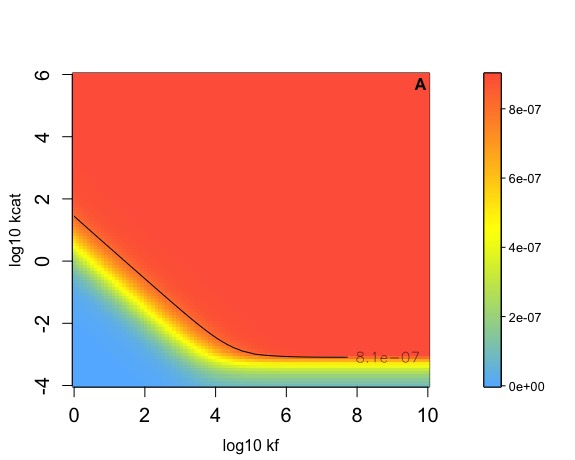
\includegraphics[scale=0.38,trim=0cm 0cm 0cm 1.5cm,clip]{pics/SM-Enzymes/Fit_Landscape2D_PD_abnormal.jpeg}
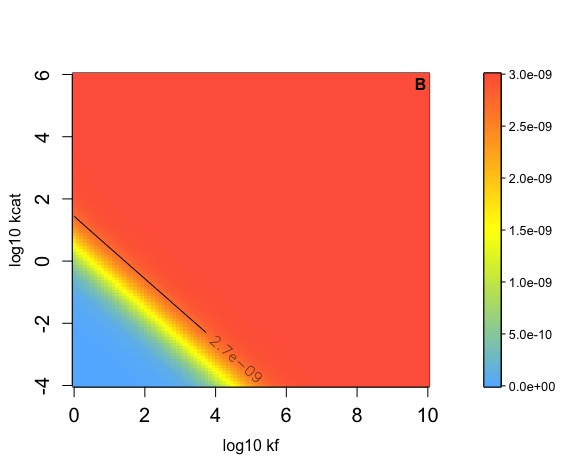
\includegraphics[scale=0.38,trim=0cm 0cm 0cm 1.5cm,clip]{pics/SM-Enzymes/Fit_Landscape2D_PD_normal.jpeg}  
\caption{Fitness landscapes for the first enzymes in pathways when uptake results from PD with $P=10^{-12}m^{-1}$\citep{Wood68,Chakrabarti94} in line with values for nucleosides or sugars for instance. The isocline corresponds to 90\% of the maximum flux. In panel A, the flux plateau is shown for an abnormally high environment nucleoside concentration ($[S_{out}]=0.15M$) -- that would be more consistent for sugars -- which allows to compare the respective landscapes for PD and FD when similar levels are reached, although the situation described for PD is thence far-fetched. The trend -- steep slope, large plateau -- is even more pronounced than for FD, because concentrations used with FD are low in comparison, which proved to move the plateau towards higher values for both kinetic parameters. In panel B, the flux is represented given the same concentration as that used with FD ($[S_{out}]=0.5mM$), showing a large plateau whose span is barely demarcated by an area sustaining a very low flux. Furthermore, the flux obtained is more than 2 orders of magnitude lower than for facilitated diffusion, suggesting that PD can only marginally contribute to nutrient uptake even under an extremely favourable scenario.}
\label{fig1-ann}
\end{figure}

\begin{figure}[htb!]
\begin{center}
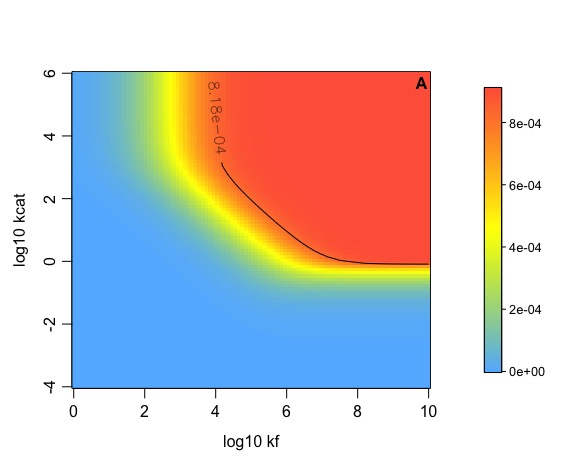
\includegraphics[scale=0.4,trim=0cm 0cm 0cm 1.5cm,clip]{pics/SM-Enzymes/Fit_Landscape2D_FD_abs_sugars.jpeg} 
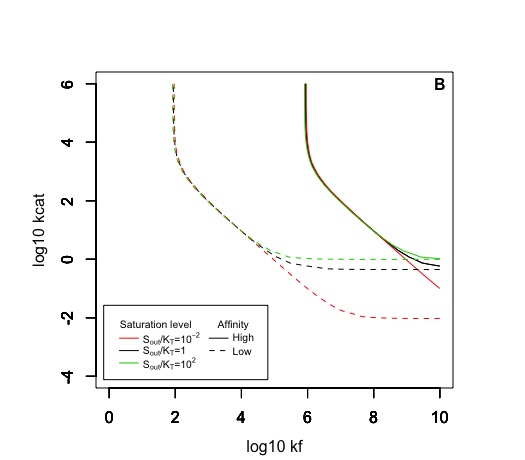
\includegraphics[scale=0.4,trim=0cm 0cm 0cm 1.5cm,clip]{pics/SM-Enzymes/2DFit_NonSatToSat_sugars.jpeg}   
\caption{Fitness landscapes for the first enzymes in pathways when uptake results from FD with sugar-like transporters ($V_{Tm}=10^{-3}M.s^{-1}$). On the right hand side (A), the absolute flux is shown for a moderate affinity and nearly saturated transporters ($[S_{out}]=10K_T$, $K_T=1mM$) to compare with absolute flux resulting from PD of sugars (see Figure \ref{fig1-ann}); the isocline corresponds to $90\%$ of the maximum achievable flux. In (B) -- where affinity is either high ($K_T=10\mu M$) or low ($K_T=0.1M$) -- the influence of the substrate concentration in the environment is represented and proven to have little or no impact also in the case of a high flux, especially when the affinity is high.}
\label{fig2-ann}
\end{center}
\end{figure}

Comparing with facilitated diffusion (FD, shown in the paper), one can see that for a similar flux (Fig \ref{fig1-ann}-A) the landscape is even flattest with PD, because of the flattening influence of high external concentrations (for a same flux level) that increase nutrient gradients. Anyhow, the substrate concentration yielding such a high level is either very unlikely to be found even within multicellular organisms -- for nucleosides/amino acids -- or still yielding very low flux relatively to FD -- for sugars -- as sugar flux are many orders of magnitude higher than nucleosides/amino acids ones (see (A) of Figure~\ref{fig2-ann} for absolute flux with sugar-like transporters). Likewise, setting the concentration to more realistic levels for nucleosides/amino acids does not alter the shape of the landscape while proving PD to be nowhere near the efficiency of FD (illustration (B) on the right of Figure~\ref{fig1-ann}). Besides, as for lower levels of flux, saturation only affects the selective pressure acting on $k_{cat}$ when transporters affinity is moderate to low.

\subsubsection{Transporters and the general shape of the fitness landscape (under FD) \label{sec:FP1}}

On Figure \ref{fig3FD-ann}, the fitness landscape of the upstream enzyme is displayed considering different kinetic parameters of transporters (summarized by the 0.9 isocline in fig.~2A of the article) that correspond to those found in living organisms. In well studied organisms, sugars correspond to the (F,I) cases -- low to moderate affinity, high flux -- and amino acids and nucleosides more or less match with (A) cases -- and to a lower degree, (B) and (D). As discussed in the paper, the maximum flux induced by transporters increases the selective pressure on both $k_{cat}$ and $k_f$ of the first enzyme, while their affinity mainly influences selection on $k_f$.

\begin{figure*}[h!]
\centering
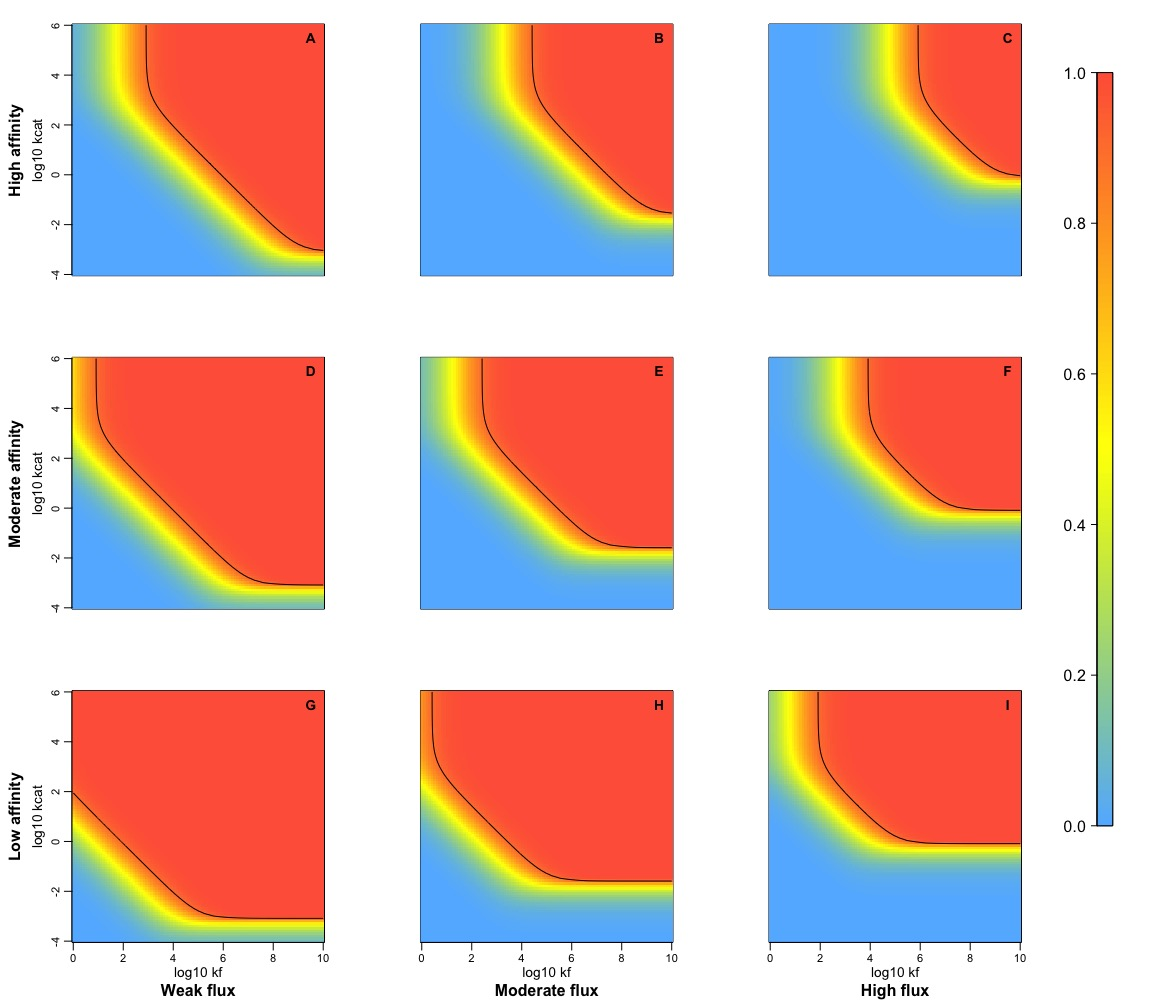
\includegraphics[scale=0.41,trim=0.2cm 0 0 0cm,clip]{pics/SM-Enzymes/Fit_Landscape2D_Sensitivity.jpeg} 
%\vspace{0.2cm}
\caption{Both the affinity and rate of a transporter have an impact on the (normalized) flux landscape for upstream enzymes, the black isocline (corresponding to $0.9$) delineates the fitness plateau. Each plot represents the landscape obtained with a pair of values for transporters affinity $K_T$ and saturation $V_{Tm}$. Moving one step to the right means that $V_{Tm}$ increases by 1.5 orders of magnitude -- from $10^{-6}$ (low flux) to $10^{-3} M.s^{-1}$ (high) -- and one step up means that $K_T$ decreases by 2 orders of magnitude, starting at $10^{-1}M$ (low affinity). Increasing $K_T$ extends the plateau only towards the left part of the landscape, allowing enzymes with lower $k_f$s on the plateau, whereas decreasing $V_{Tm}$ extends the plateau in both directions. Other parameter values are : $k_r=1000/s$, $[E_{tot}]=1mM$ and $[S_{out}]=10 \times K_T$.}
\label{fig3FD-ann}
\end{figure*}

\subsubsection{Fitness landscape of the second enzyme (under FD)\label{sec:FP2}}

\noindent\paragraph{Fitness landscapes with a degradation rate}

On Figure \ref{fig3-ann}, concentrations of the first product are represented as functions of the second enzyme parameters, perfectly matching flux landscapes displayed in the article down to the details of the shape. Predictably, it shows that the degradation rate exerts an apparent influence once and only once metabolite concentrations start to rise and their product with the degradation rate approach the level of flux achieved within the pathway (slightly below $10^{-6}M$). Indeed, at steady-state, if the next enzyme is very inefficient, almost exactly the flux of newly formed product is degraded, which means that $\eta_d [P_1]^*\approx \Phi_{P_1}$, yielding $[P_1]^*\approx\Phi_{P_1}/ \eta_d$.



\begin{figure}[htb!]
\centering
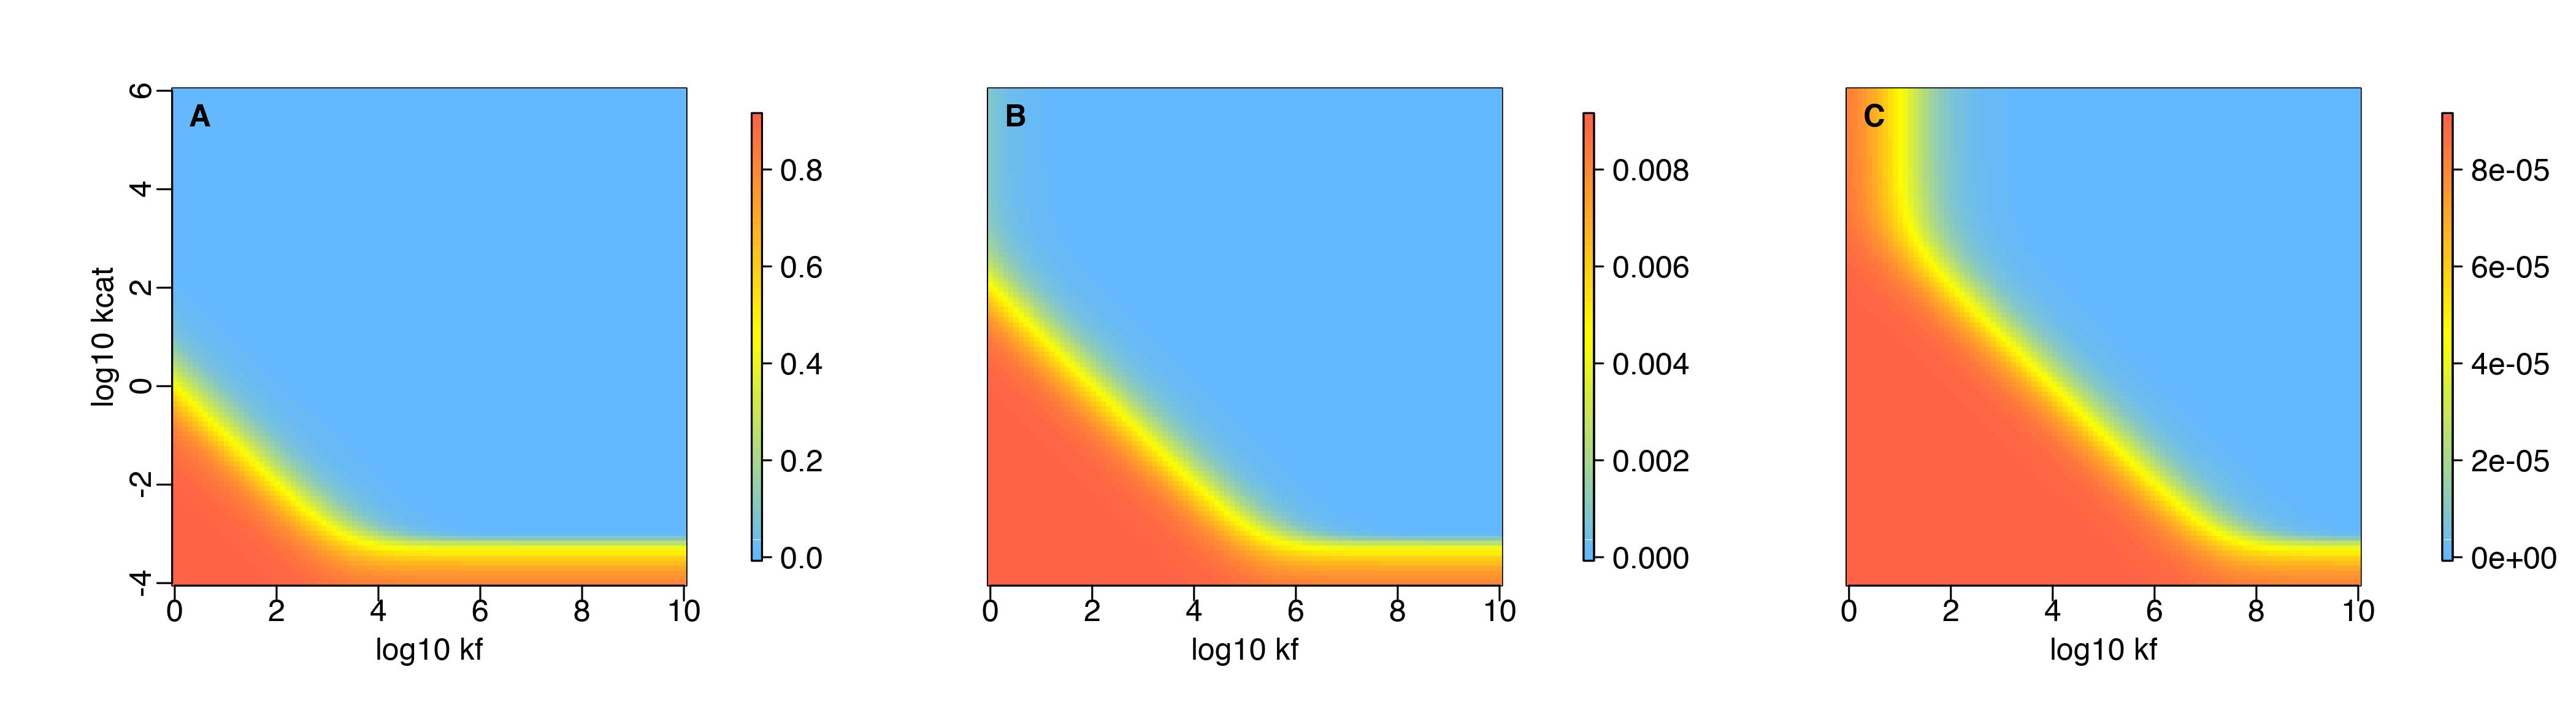
\includegraphics[scale=0.46,trim=1cm 0cm 0cm 1cm,clip]{pics/SM-Enzymes/2DConcentrationLandscape_degrates.jpeg} 
\vspace{-0.3cm}
\caption{Concentrations (unit: M) of the product of the first reaction for three degradation rates are plotted as functions of second enzyme kinetic parameters, for the model case of nearly saturated amino-acids like transporters ($\displaystyle V_{Tm}=1 \mu M/s$, $\displaystyle K_T=50\mu M$ and $\displaystyle [S_\text{out}]=10K_T$). The first enzyme is assumed to be perfect and highly concentrated ($k_f=10^{10}M^{-1}s^{-1}$, $k_{cat}=10^6s^{-1}$, $k_r=10^3s^{-1}$, $[E_{tot}]=10^{-3}M$). In (A), the degradation rate is set to $\eta_d=10^{-6}s^{-1}$ and limits the intracellular concentration of product to $[P_{1}]=1M$, while in (B) and (C), these values are respectively $\eta_d=10^{-4}s^{-1}$ and $10^{-2}s^{-1}$ limiting it to $[P_{1}]=10^{-2}M$ and $[P_{1}]=10^{-4}M$.}
\label{fig3-ann}
\end{figure}

\begin{figure}[htb!]
\centering
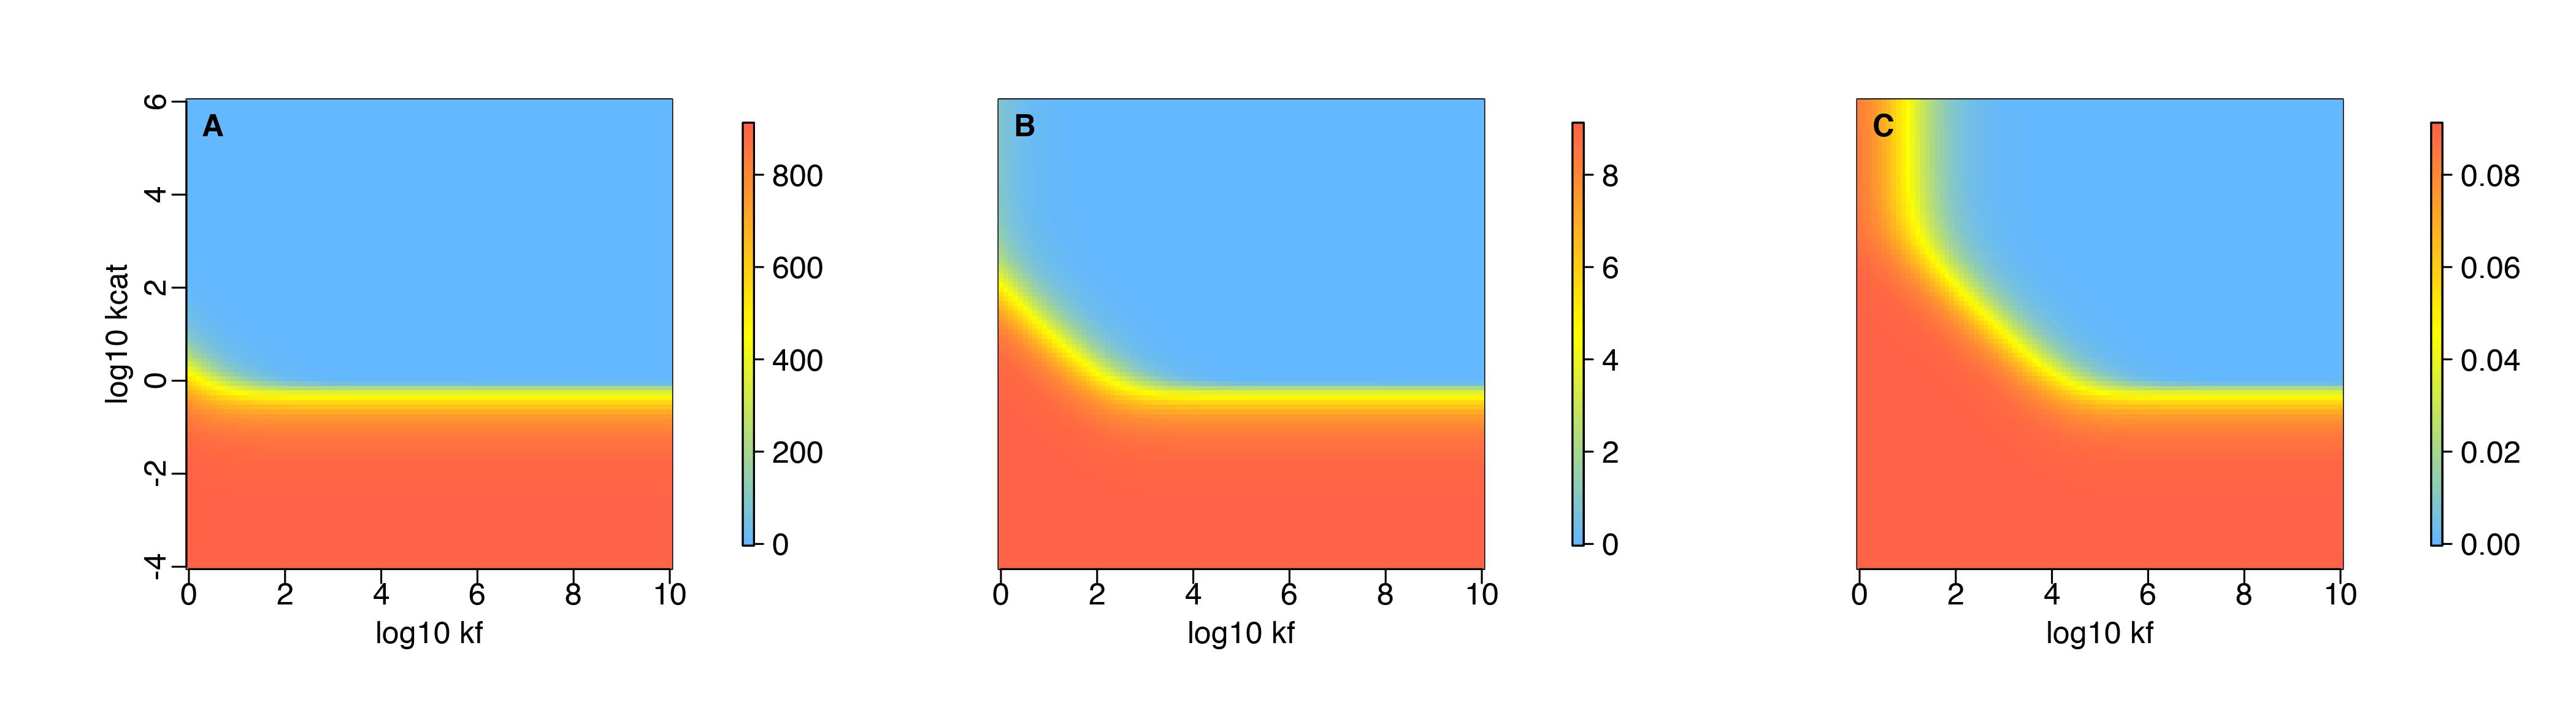
\includegraphics[scale=0.46,trim=1cm 0cm 0cm 1cm,clip]{pics/SM-Enzymes/2DConcentrationLandscape_degratesHF.jpeg} 
\vspace{-0.3cm}
\caption{Concentrations (unit: M) of the product of the first reaction for three degradation rates are plotted as functions of second enzyme kinetic parameters, for the model case of nearly saturated sugar like transporters ($\displaystyle V_{Tm}=1 mM/s$, $\displaystyle K_T=5 mM$ and $\displaystyle [S_\text{out}]=10K_T$). The first enzyme is assumed to be perfect and highly concentrated ($k_f=10^{10}M^{-1}s^{-1}$, $k_{cat}=10^6s^{-1}$, $k_r=10^3s^{-1}$, $[E_{tot}]=10^{-3}M$). In (A), the degradation rate is set to $\eta_d=10^{-6}s^{-1}$ and limits the intracellular concentration of product to $[P_{1}]=10^3M$, while in (B) and (C), these values are respectively $\eta_d=10^{-4}s^{-1}$ and $10^{-2}s^{-1}$ limiting it to $[P_{1}]=10^{1}M$ and $[P_{1}]=10^{-1}M$. As the first two concentrations (A and B cases) cannot be reached without completely compromising a cell's viability, only the higher one is considered to compare with the first enzyme (fitness landscape in Figure \ref{fig4-ann}) along with two higher degradation rates limiting concentration to $[P_{1}]=10^{-2}M$ and $[P_{1}]=10^{-4}M$, the same amount than in the case of amino acids with the upper degradation rates.}
\label{fig4a-ann}
\end{figure}

\begin{figure*}[h!]
\begin{center}
\begin{minipage}[c]{0.52\linewidth}
%\hspace{0.75cm}
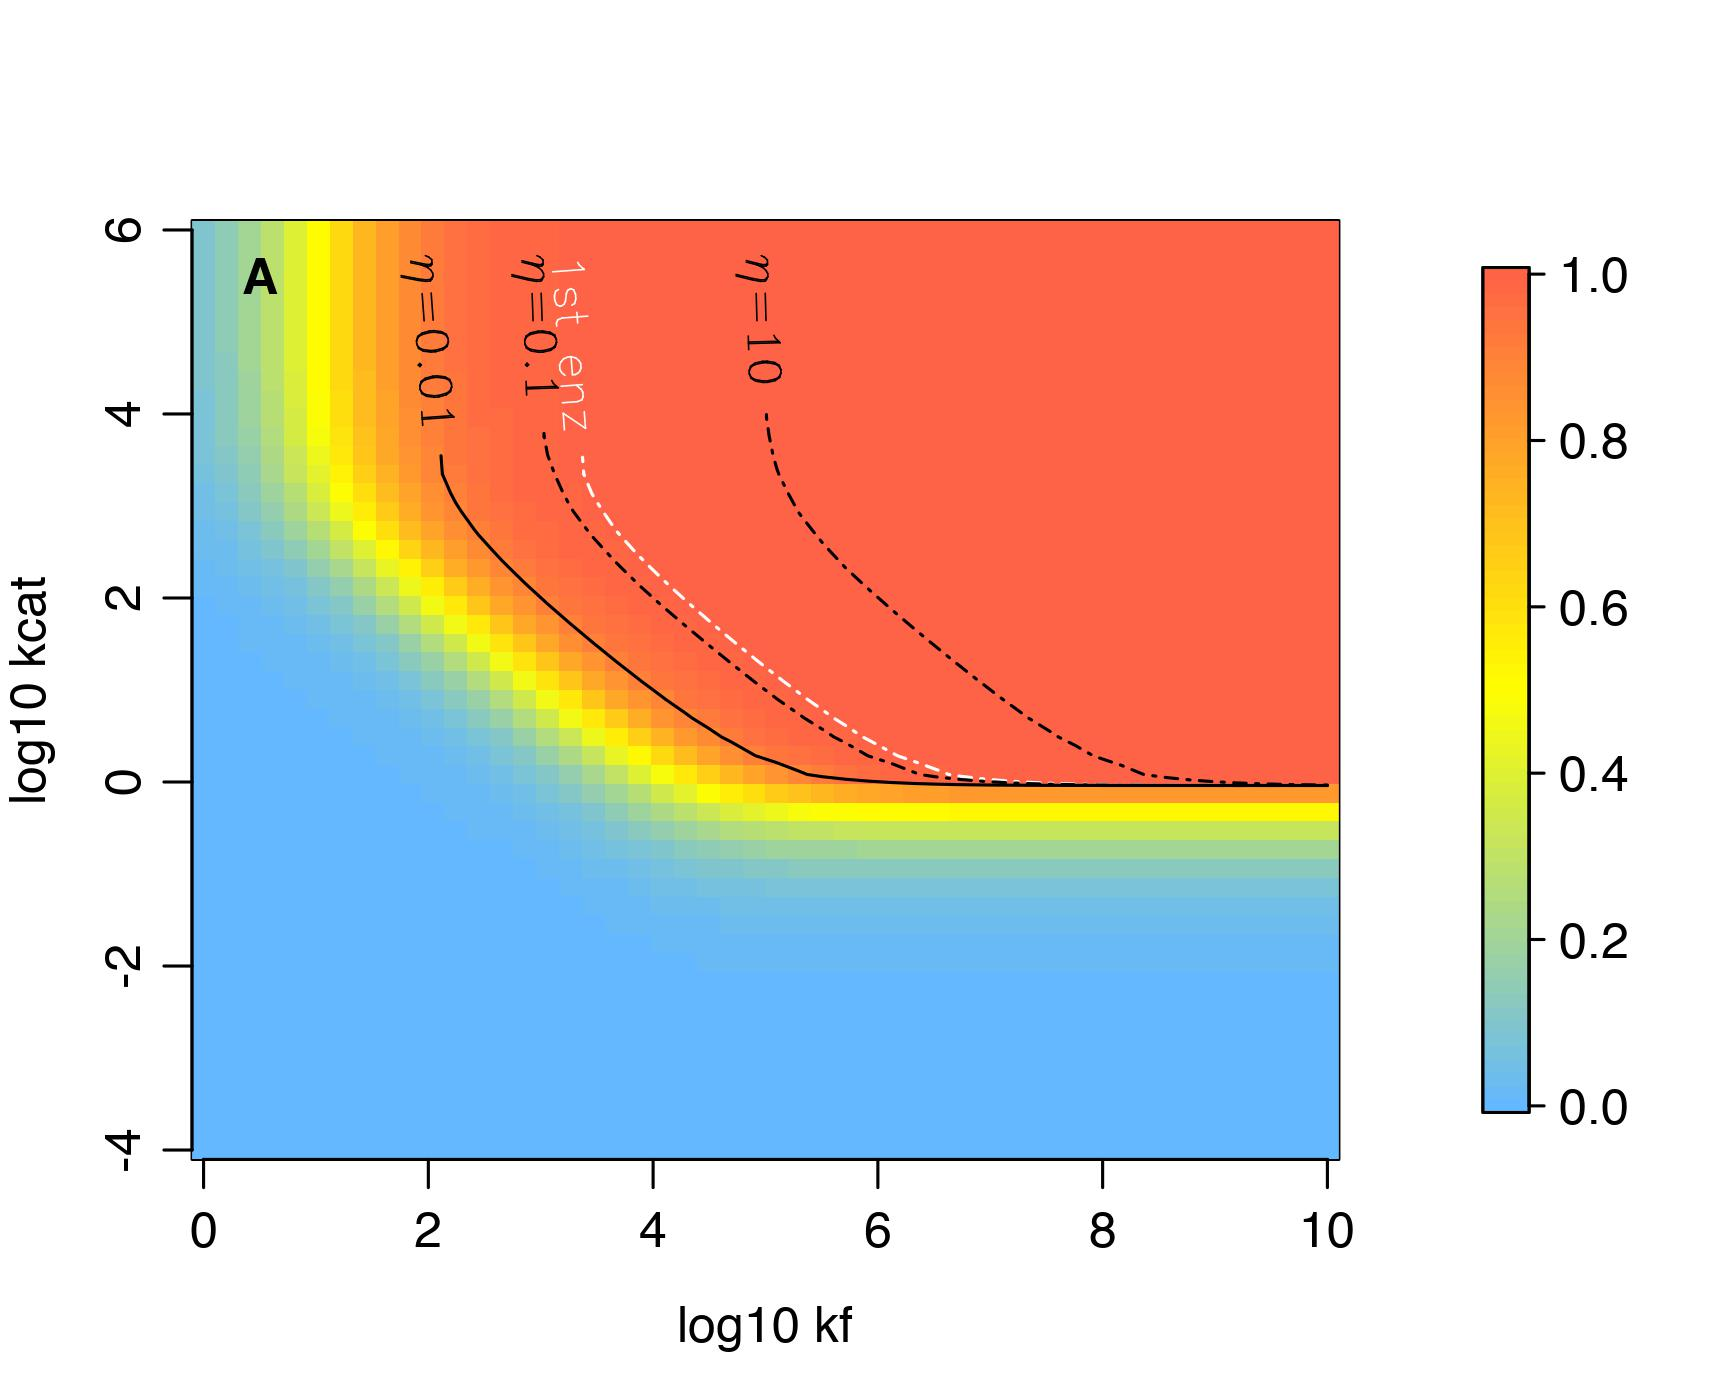
\includegraphics[scale=0.55]{pics/SM-Enzymes/2DFitLandscape_etahigh_noreverse_HF.jpeg} 
%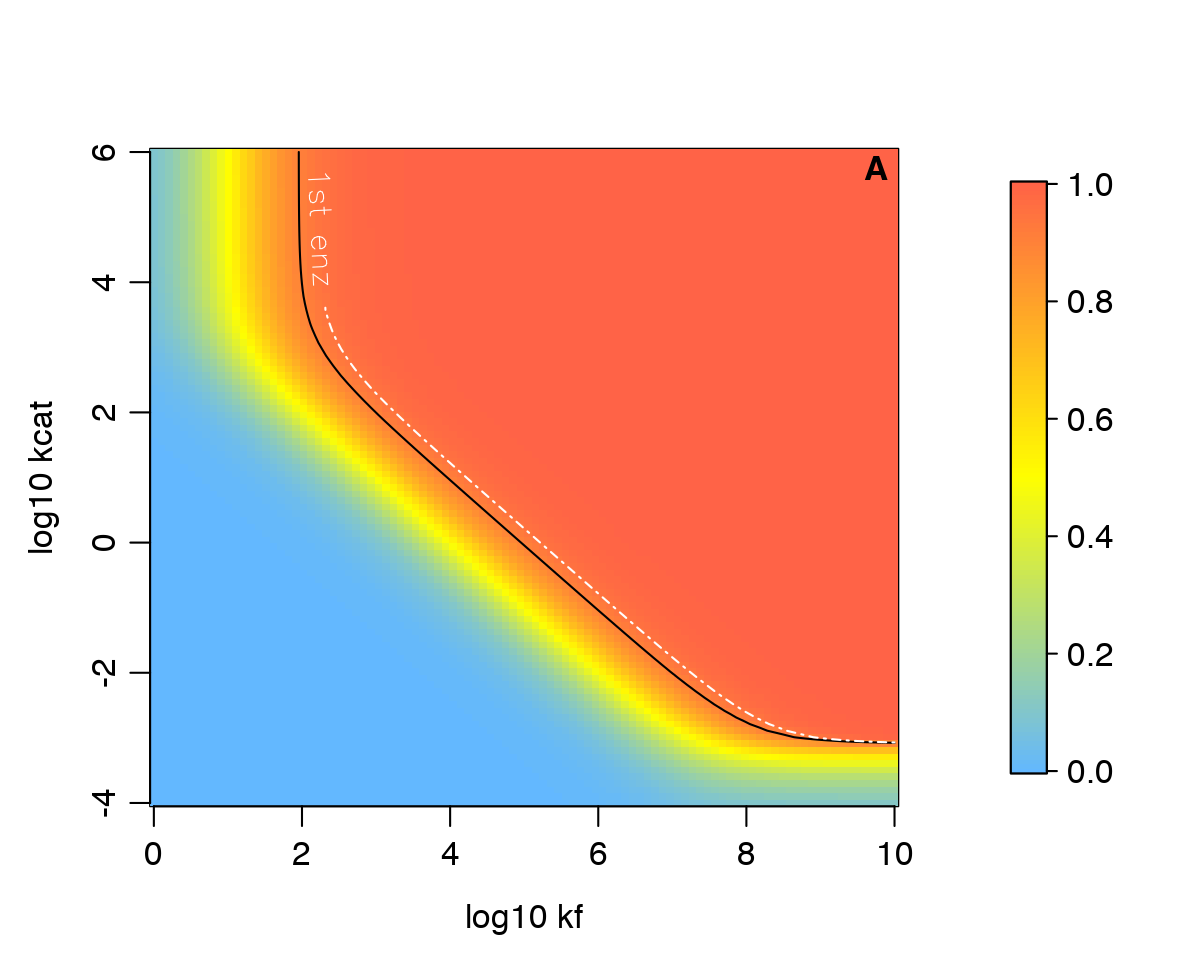
\includegraphics[scale=0.5]{Figures/2DFitLandscape_etahigh_noreverse.png} 
\end{minipage} \hfill
%\hspace{0.3cm}
\begin{minipage}[c]{0.47\linewidth}
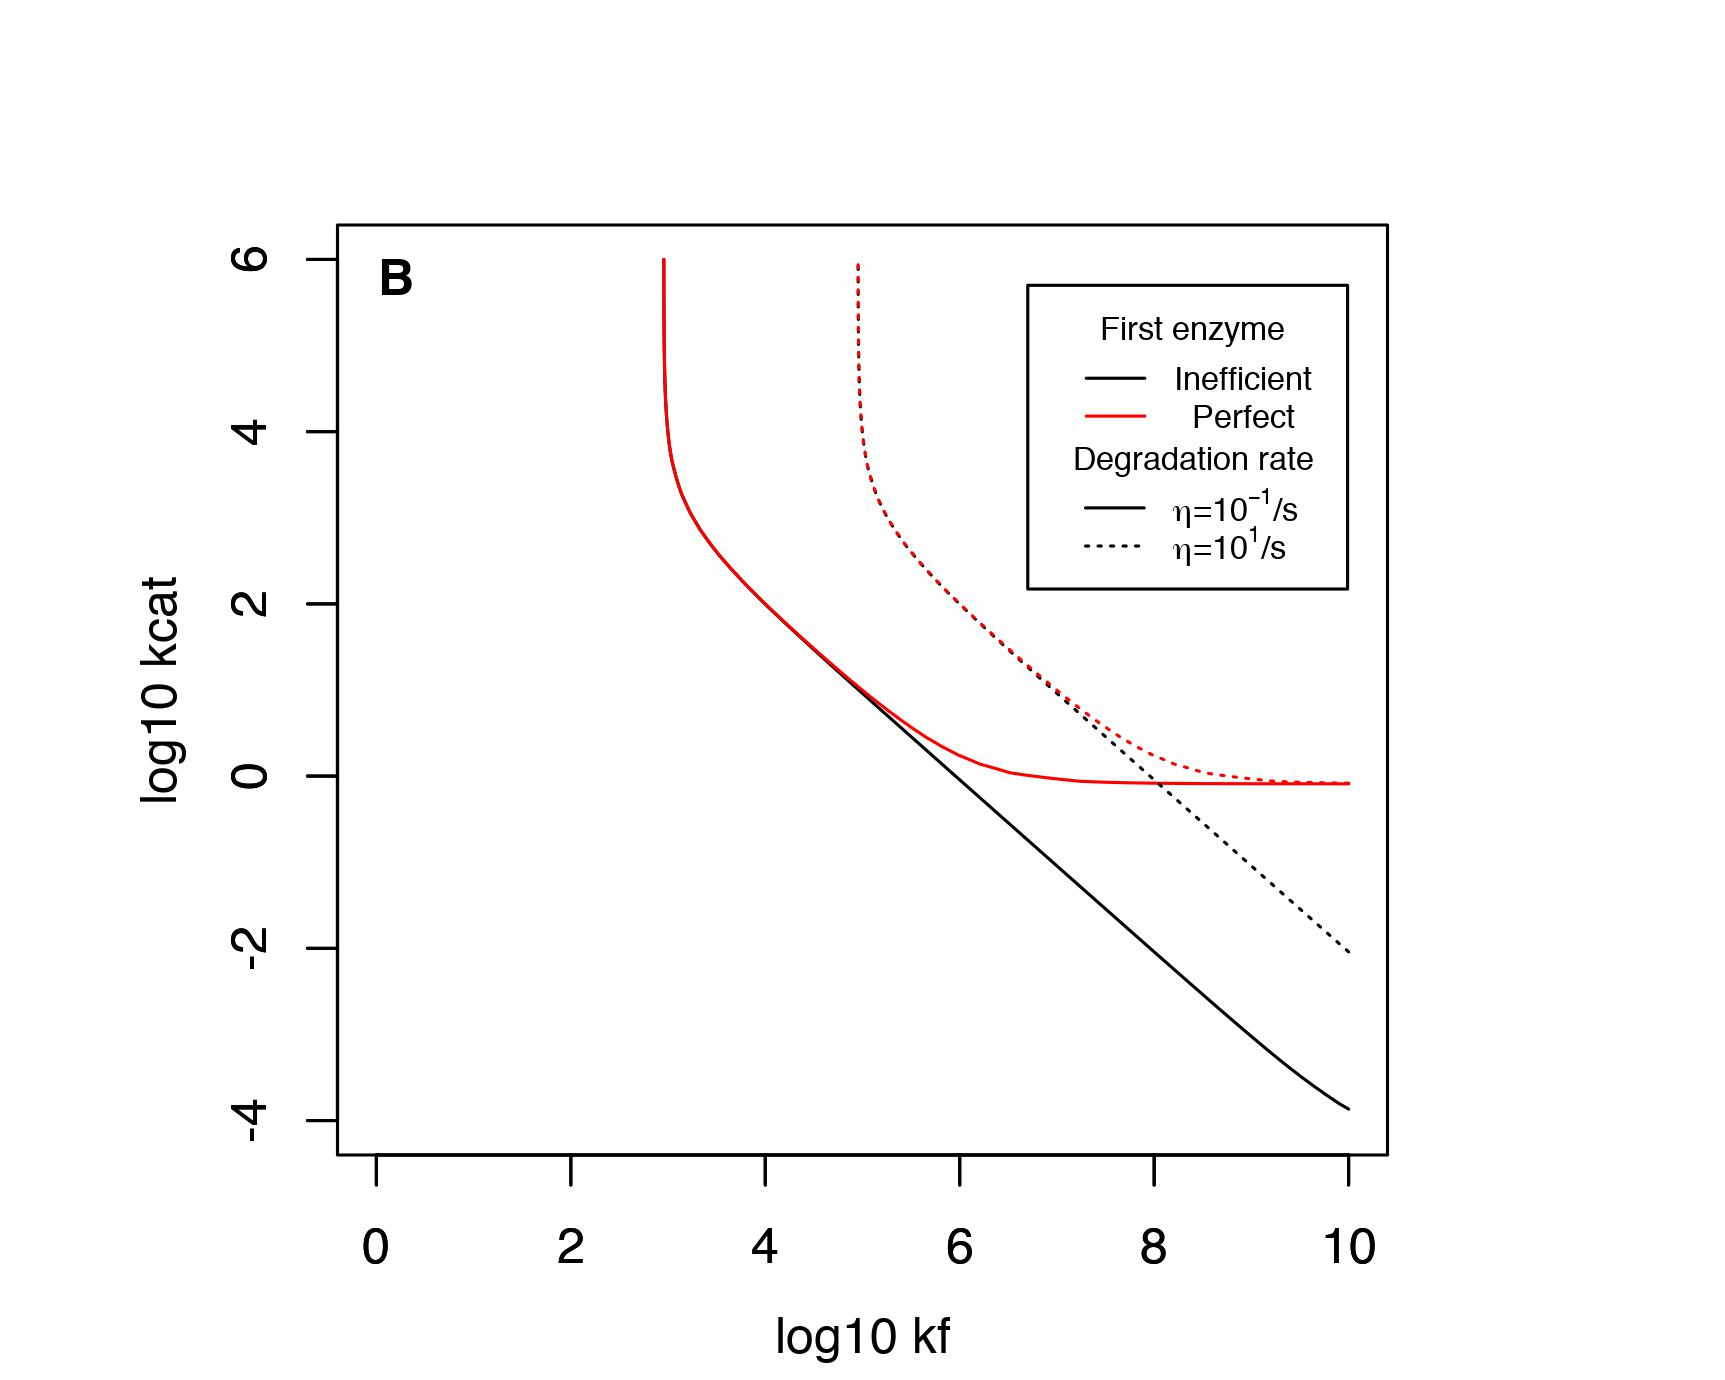
\includegraphics[scale=0.55]{pics/SM-Enzymes/2DFit_Landscape_2Enz_First_Enz_Influence_HF.jpeg} 
%\includegraphics[scale=0.42,trim=10 0 0 0,clip]{Figures/2DFit_Landscape_2Enz_First_Enz_Influence.jpeg} 
\end{minipage}
%\vspace{-0.3cm}
\caption{Fitness landscapes for the second enzyme in the context of an irreversible pathway (no backwards flux for the first reaction). These enzymes are involved in a high flux pathway whose pace is driven by $\displaystyle V_{Tm}=1 mM/s$, $\displaystyle K_T=5mM$ and $\displaystyle [S_\text{out}]=10K_T$. Constant settings for both enzymes also correspond to the model case with $k_r=1000s^{-1}$ and $ [E_{tot}]=1mM$. (A) shows the fitness landscape for a rather low degradation rate (for the case of sugars) limiting $[P_1]$ to $10^{-1}M$ when the upstream enzyme is perfect and concentrated ($k_f=10^{10}M^{-1}.s^{-1}$, $k_{cat}=10^6s^{-1}$), and constrasts this landscape with that for two higher degradation rates limiting concentration to $[P_{1}]=10^{-2}M$ and $[P_{1}]=10^{-4}M$. Predictably, the isocline moves toward upper $k_f$s. Besides, contrasting these landscapes with that of the first enzyme shows that they are rather similar. Plateau isoclines drawn in (B) show results for the two higher degradation rates, in the context of an upstream concentrated enzyme being either perfect (see above) or inefficient ($k_f=10^{2}M^{-1}.s^{-1}$, $k_{cat}=10^{-2}s^{-1}$, $k_r=10^3s^{-1}$). Decreasing $\eta_d$ still makes the cell tolerant to higher concentrations of intermediate metabolites (the product of the first reaction), while the efficiency of the first enzyme only influences the pressure on $k_{cat}$ if high intracellular concentrations are not toxic.}
\label{fig4-ann}
\end{center}
\end{figure*}

Equilibrium concentrations for sugars are higher for similar degradation rates because the influx is larger (see Figure \ref{fig4a-ann}) - the increase being proportional to that of the flux. If the absolute concentration -- instead of the relative cost -- matters then the constant $\eta_d$ may be higher for sugars (thereby reaching biologically relevant metabolite concentrations). %We have represented the metabolite concentration of the intermediate product in Figures.~.\ref{fig3-ann} and \ref{fig4a-ann} to confirm that with the same degradation rate, the maximum concentraito

%The considerations above stand for linear cost functions; when the fitness is instead penalized by a non linear toxicity function (see next subsection, Figures \ref{fig4b-ann} and \ref{fig4c-ann})... but to enable the comparison with the case of amino acids, we show on Figure \ref{fig4-ann} results for concentrations limited to the same amount than in the case of amino acids shown in FIG.3 of the paper (by multiplying each $\eta_d$ by a factor $10^3$ corresponding to the differences between the two maximum fluxes). 


Degradation rates modulate the fitness landscapes of the second enzyme. One remarkable phenomenon here is that the landscape does not depend much on the efficiency of the first enzyme : this is especially true for $k_f$, whose selective pressure is mostly insensitive to the first enzyme efficiency (or the level of flux, more generally). For a system where a specific flux of metabolite $\Phi$ can either be converted through a chemical reaction with a dedicated enzyme or degraded, it can be shown that the relative loss of fitness incurred by a change in $k_f$ does not depend on $\Phi$ when $\Phi<<k_{cat}[E_{tot}]$ (see Mathematical appendix for the proof, where $V_m=k_{cat}[E_{tot}]$). This explains that the location of the fitness landscape for the second enzyme in this case scarcely depends on the previous enzyme.

The flux of product that the second enzyme needs to process depends on the interplay between the first intracellular enzyme, the degradation rate and transmembrane transporters. To test the selective influence of the latter on the second enzyme, we plotted the landscape of the second enzyme for different degradation rates and first enzyme efficiencies when the pathway is initiated by sugar-like transporters, showing that the processes studied follow similar trends than with transporters involved in lower fluxes (see Figure \ref{fig4-ann} for sugars, to contrast with landscapes for lower fluxes found in Fig.~3 of the article).

\noindent\paragraph{Fitness landscapes with a non-linear toxicity function}

\begin{figure}[htb!]
\centering
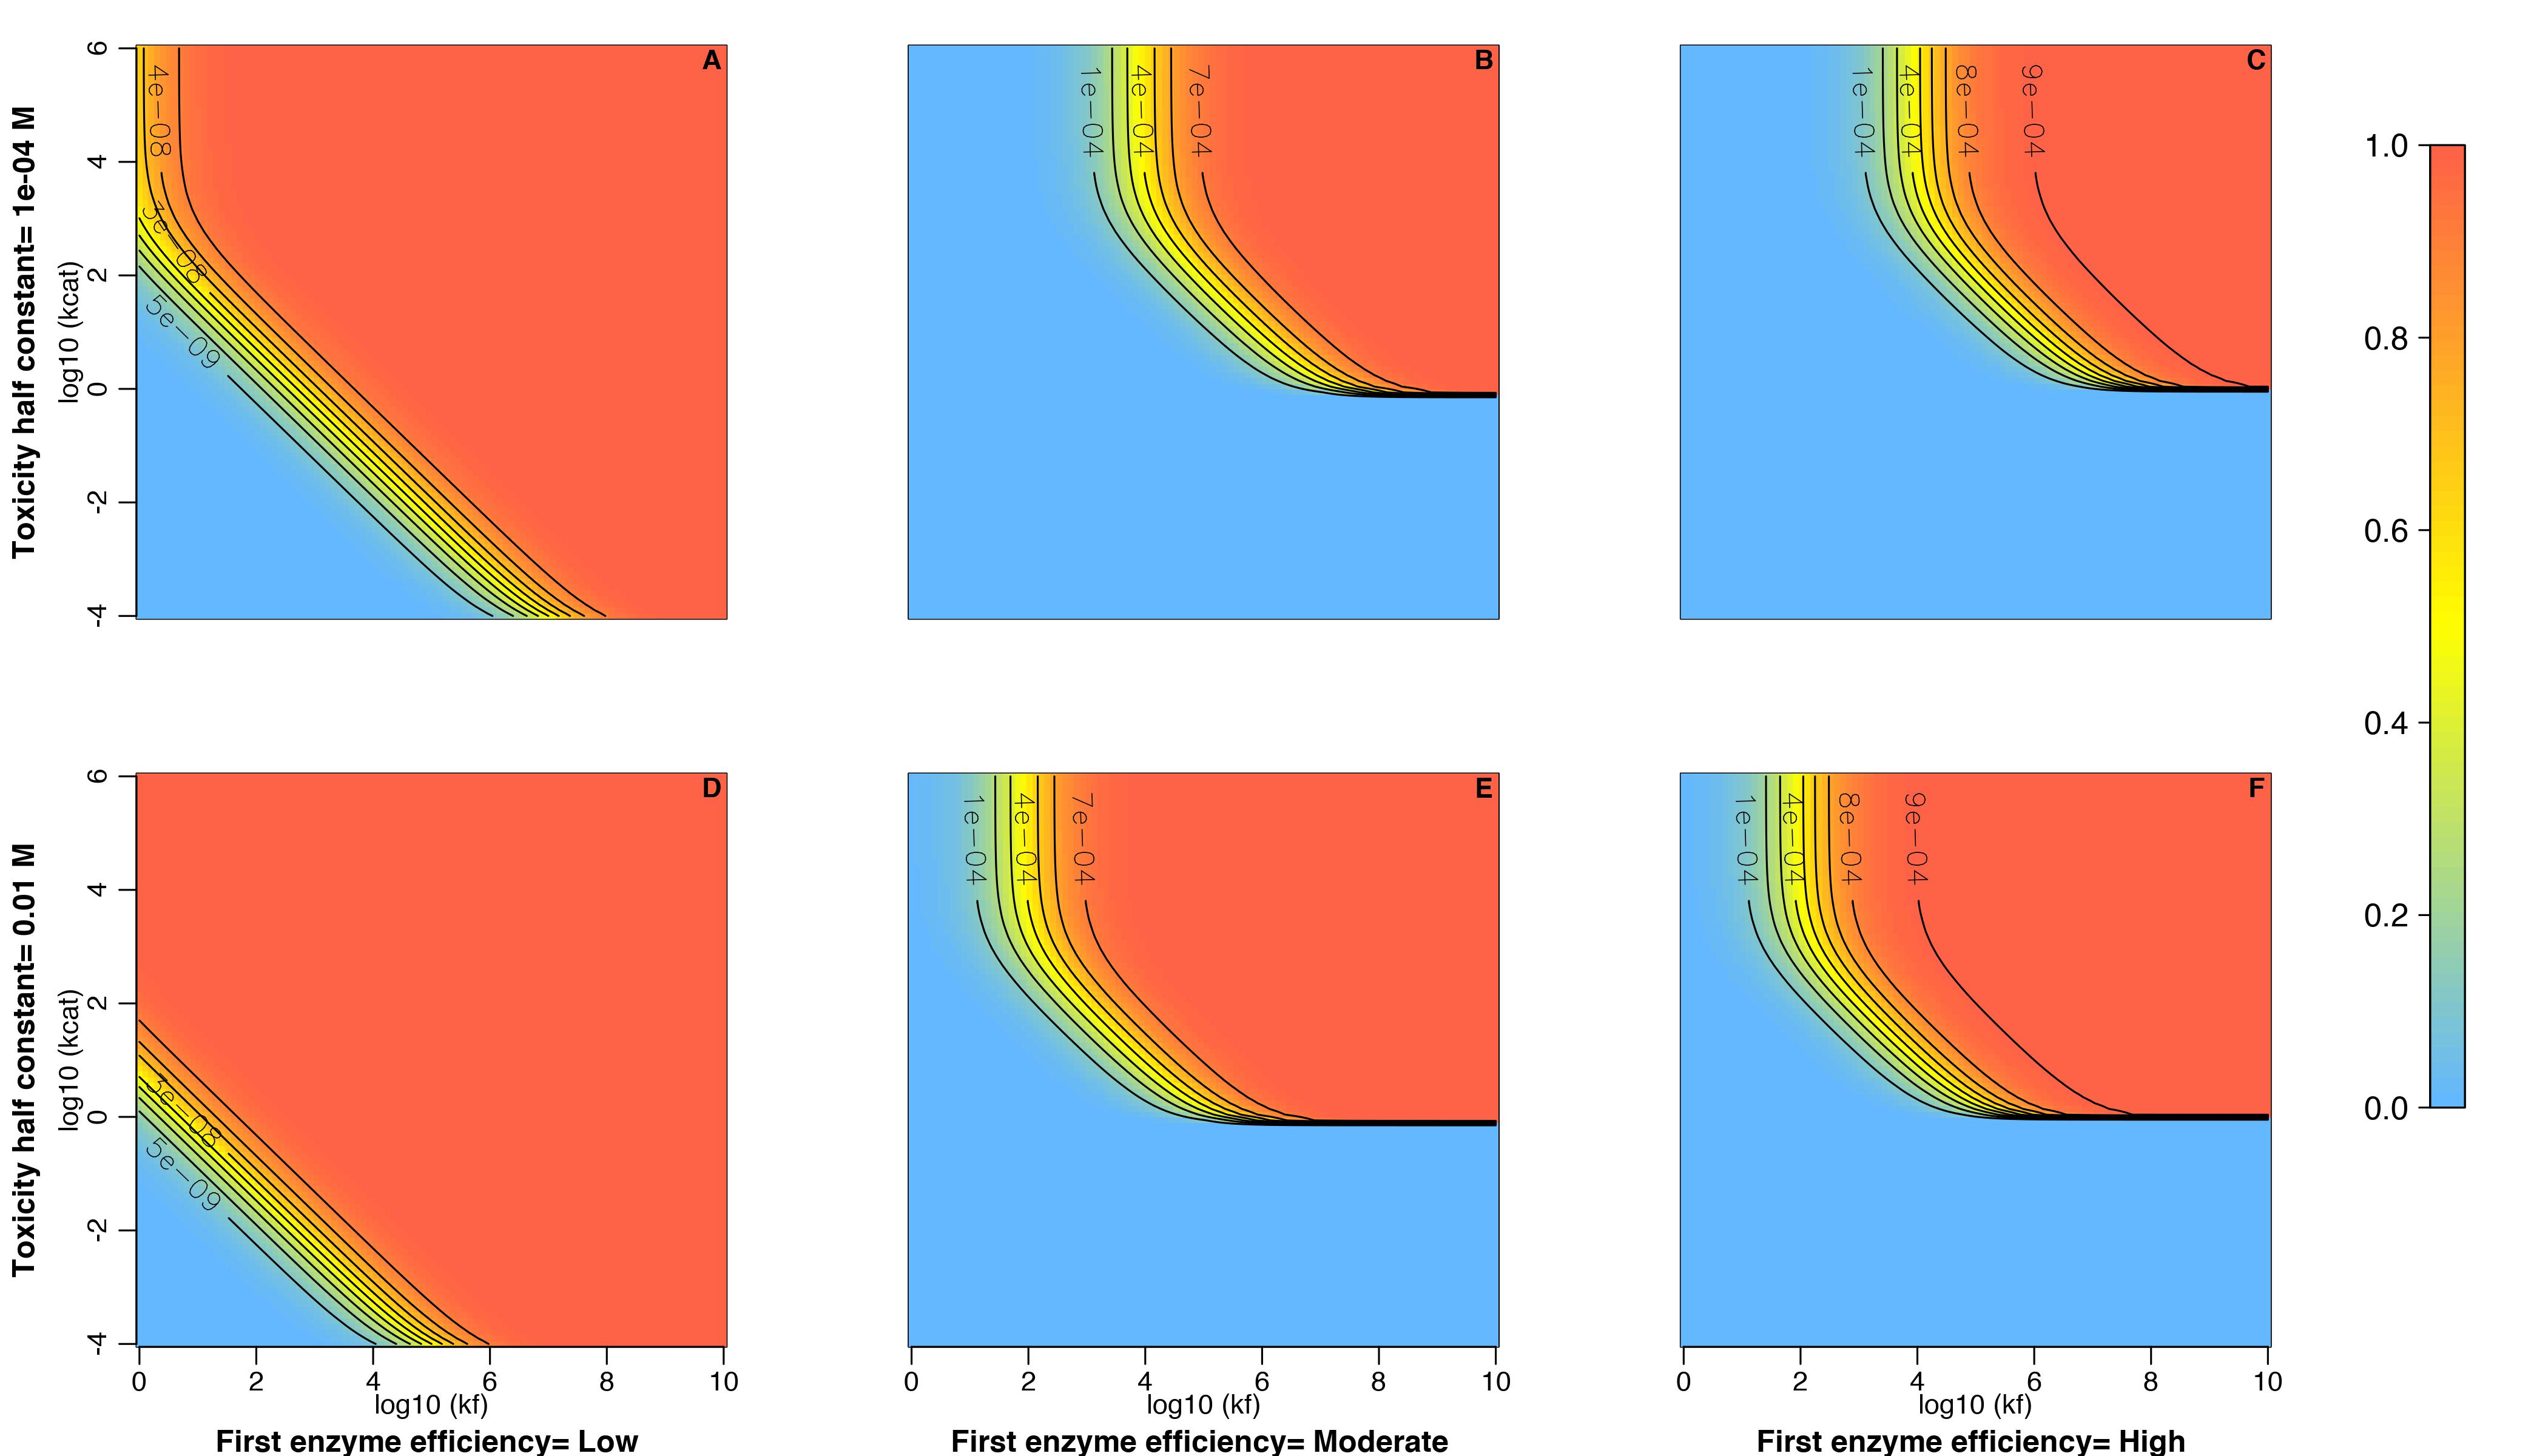
\includegraphics[scale=0.46,trim=0cm 0cm 0cm 0cm,clip]{pics/SM-Enzymes/2DFit_Landscape_2Enz_First_Enz_Influence&Tox.jpeg} 
%\vspace{-0.3cm}
\caption{Fitness landscapes for the second enzyme in a pathway when different metabolite toxicity $T$ and first enzyme efficiencies (low : $k_f=10^2 M^{-1}s^{-1}$, $k_{cat}=10^{-2}s^{-1}$; moderate : $k_f=10^5M^{-1}s^{-1}$, $k_{cat}=10^1s^{-1}$; high : $k_f=10^{10}M^{-1}s^{-1}$, $k_{cat}=10^6s^{-1}$) are considered. The case presented here is that of sugar-like transporters ($V_{Tm}=1mM s^{-1}$ and $K_T=5mM$). Note that other kinetic parameters are still $[E_{tot}]=10^{-3}M$, $k_r=10^3s^{-1}$ and no reaction reversibility $K_{eq} = 0$. As a bad first enzyme diminishes the flux by several orders of magnitude, the fitness landscape of the second enzyme already flattens for low kinetic values and the influence of toxicity is marginal. On the contrary, the moderately and highly efficient first enzymes give rise to similar fitness landscapes for the second enzyme because they generate relatively similar levels of flux : this is true for both toxicity constants (see Figure \ref{fig4c-ann} for a direct comparison based on relative fitness isoclines), with a linear relationship between the toxicity concentration and the location of the plateau. The fact that the location of the plateau is only determined by the amount of metabolite an enzyme has to process and the cellular tolerance to high concentrations indicates that it applies for any enzyme downstream the first two ones, as expected.}
\label{fig4b-ann}
\end{figure}

\begin{figure}[h!]
\centering
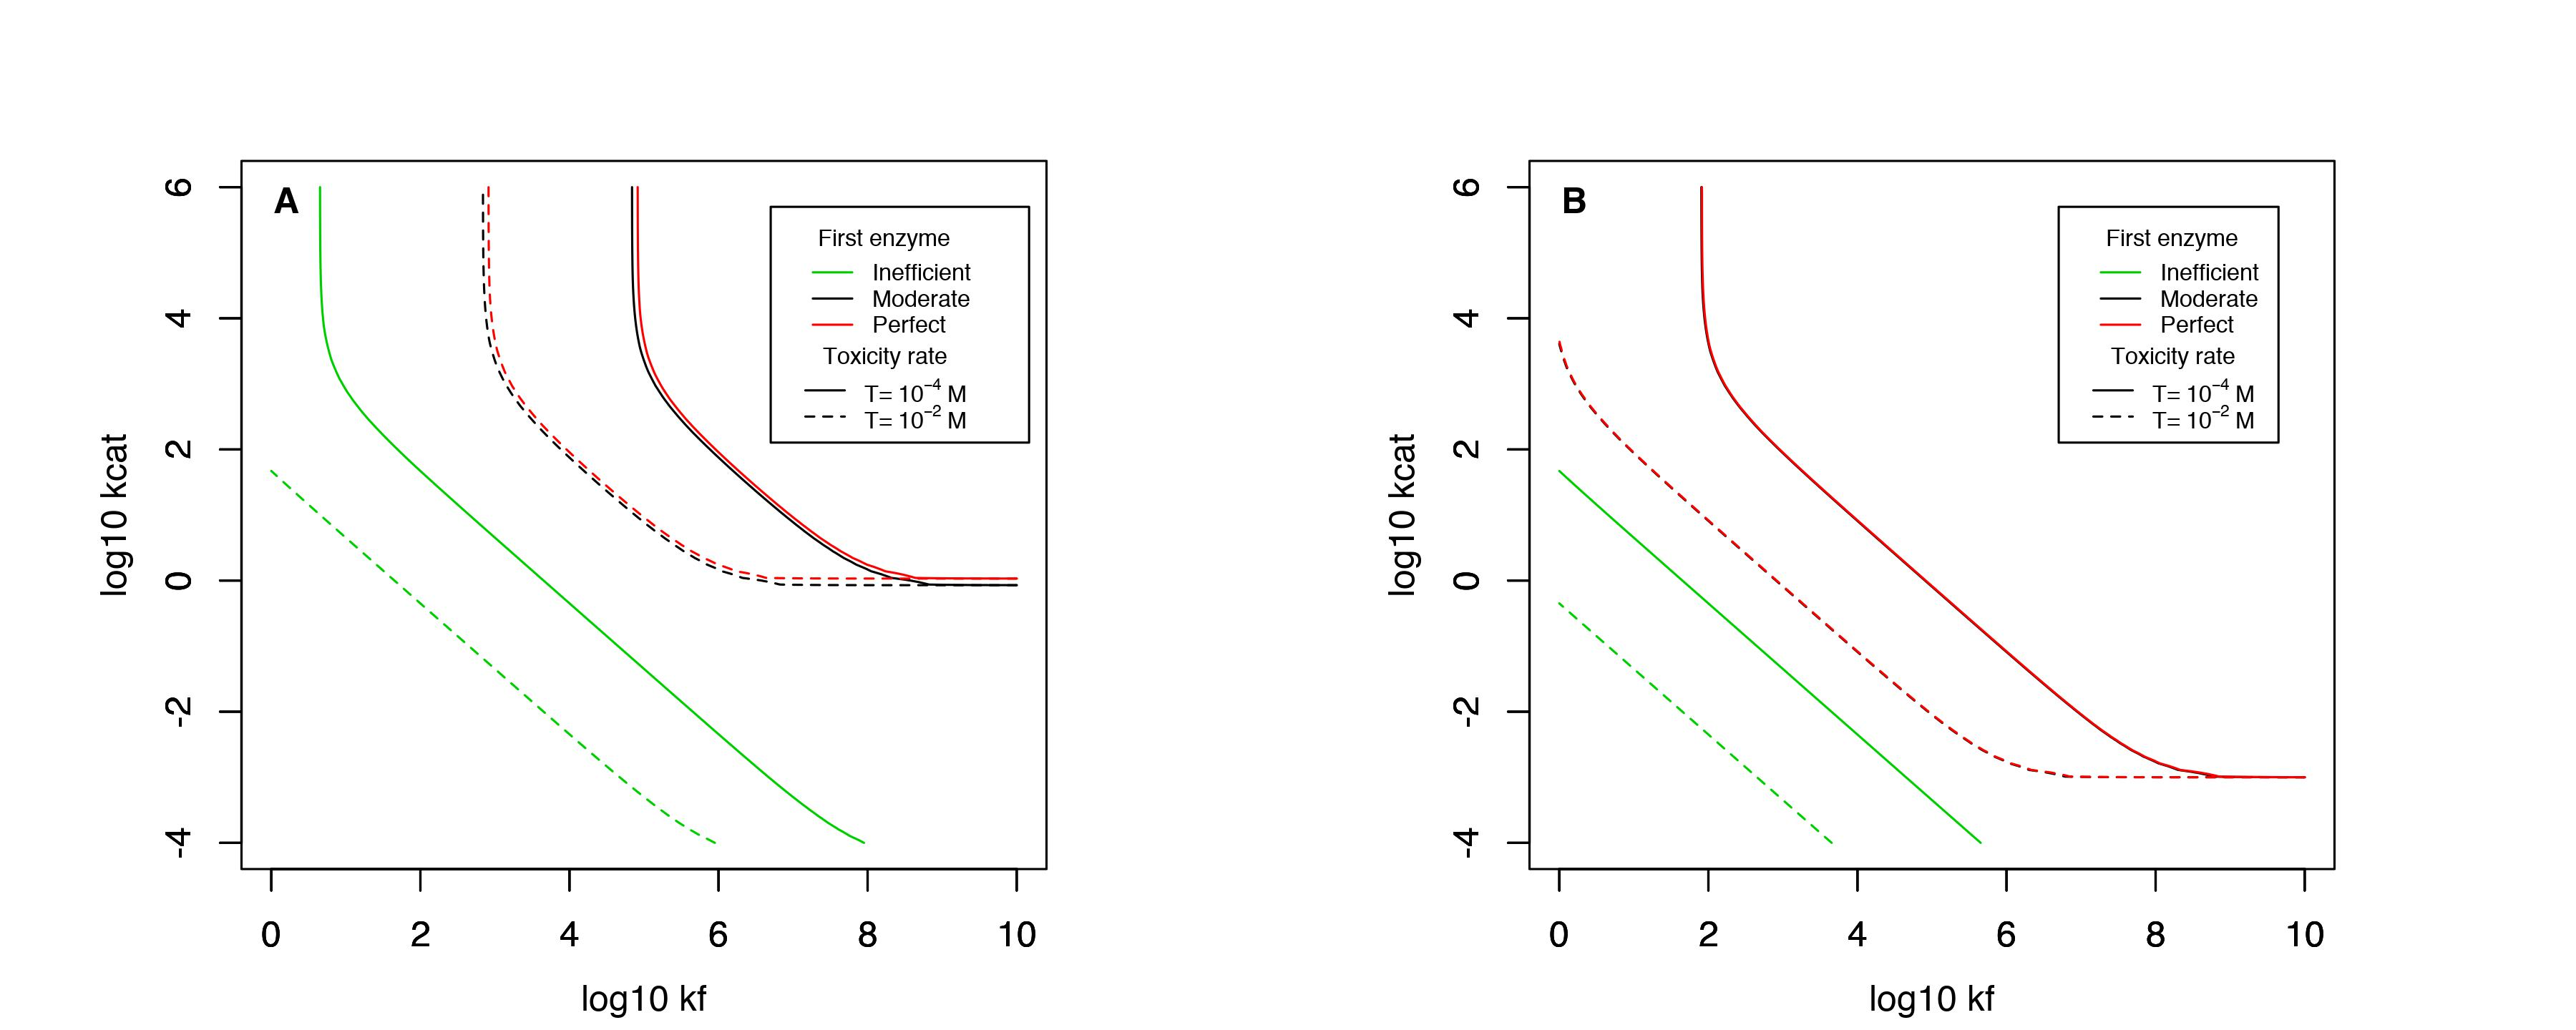
\includegraphics[scale=0.46,trim=0cm 0cm 0cm 0cm,clip]{pics/SM-Enzymes/2DFit_Landscape_2Enz_First_Enz_Influence_Tox_Allflux.jpeg} 
%\vspace{-0.3cm}
\caption{Fitness landscapes (depicted by the 0.9 isoclines) for the second enzyme in a pathway when different metabolite toxicities $T$ and first enzyme efficiencies (low : $k_f=10^2M^{-1}s^{-1}$,$k_{cat}=10^{-2}s^{-1}$; moderate : $k_f=10^5M^{-1}s^{-1}$,$k_{cat}=10^1s^{-1}$; high : $k_f=10^{10}M^{-1}s^{-1}$,$k_{cat}=10^6s^{-1}$) are considered. Note that other kinetic parameters are still $[E_{tot}]=10^{-3}M$, $k_r=10^3s^{-1}$ and neither reaction reversibility ($K_{eq} \approx 0$) nor degradation rate ($\eta_d=0$) are considered to show the effect in isolation from the other ones. (A) represents the cases of Figure \ref{fig4b-ann} for which we see that the isoclines showing the level of flux were partly misguiding since the fitness landscapes are in fact complletely superimposable for the cases of a moderately and highly efficient first enzyme. The exact same pattern is found on (B) which represents the case of amino acids like transporters ($V_{Tm}=10^{-6}M$, $K_T=50\mu M$). In any case, toxicity proved to display a similar influence, although the shift depends on the level of the flux as shown in Fig. \ref{fig4b-ann}. Still, the influence of the first enzyme is different with this form of toxicity than with a linear degradation rate, because the level of flux henceforth matters, which was mostly not the case previously for $k_f$ (see text for the demonstration).}
\label{fig4c-ann}
\end{figure}

\begin{figure}[h!]
\centering
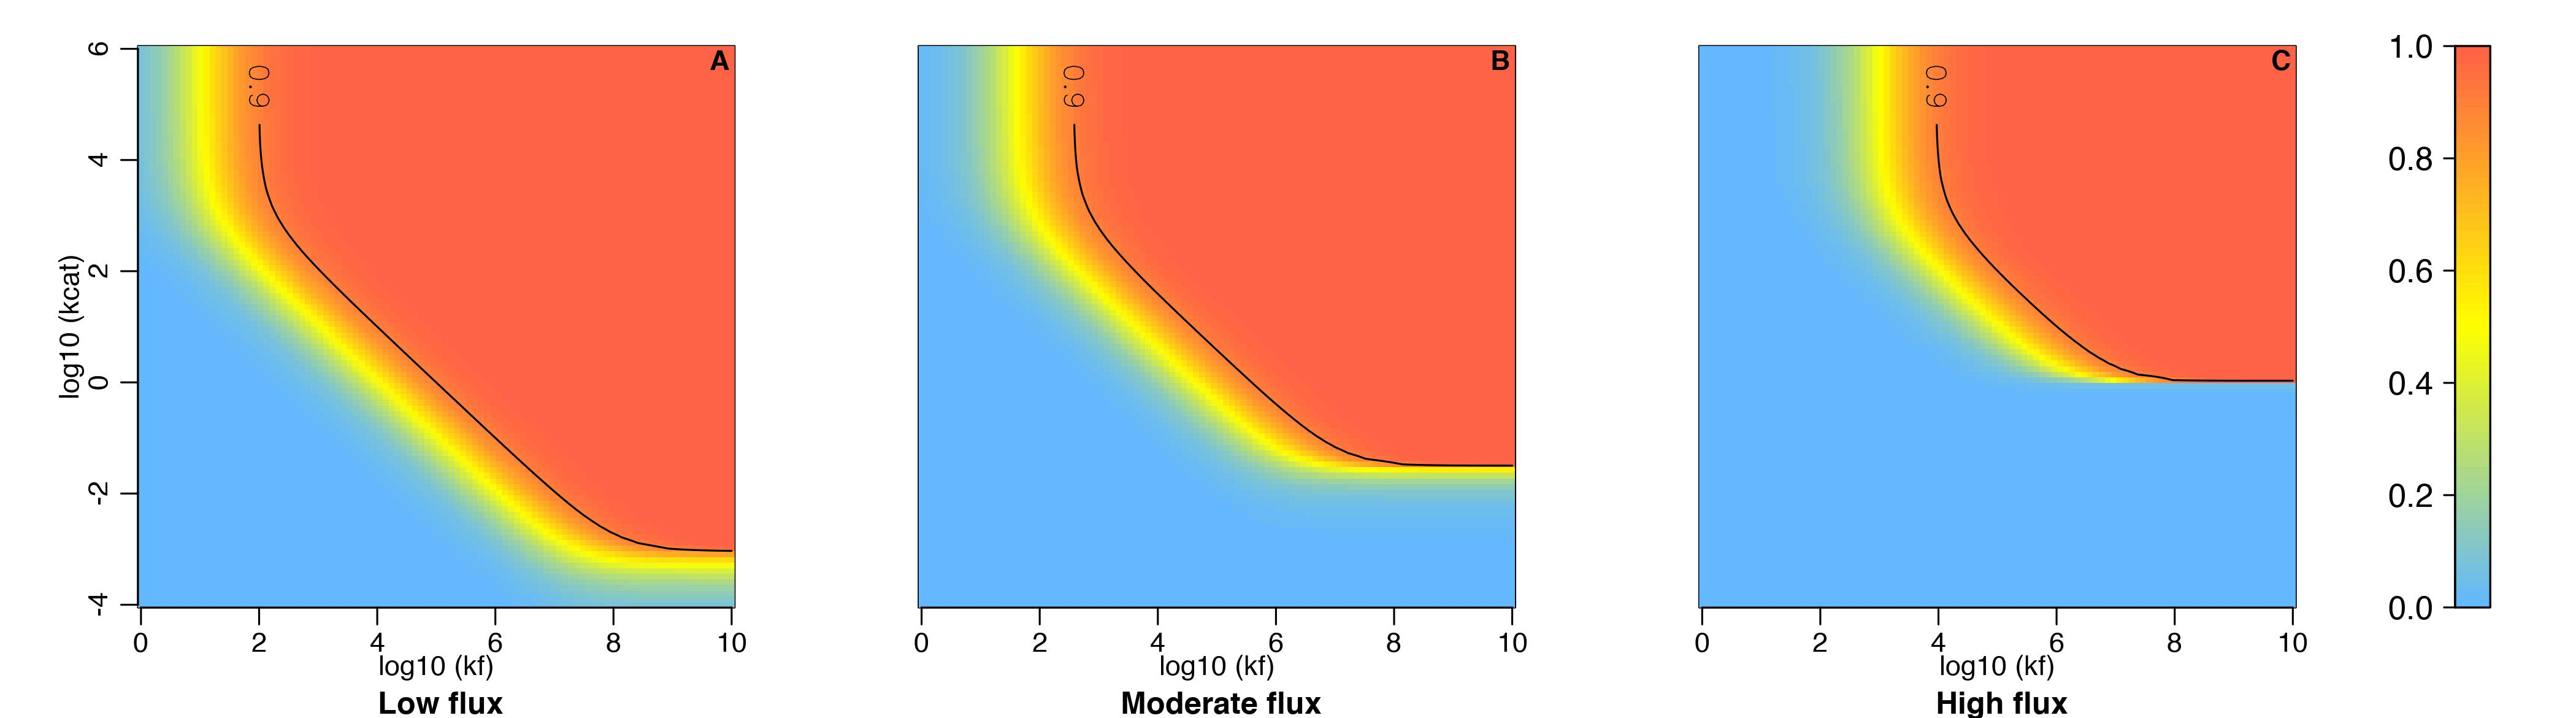
\includegraphics[scale=0.46,trim=0cm 0cm 0cm 0cm,clip]{pics/SM-Enzymes/2DFit_Landscape_2Enz_First_Enz_GenFlux&Tox.jpeg} 
%\vspace{-0.3cm}
\caption{Fitness landscapes of any enzyme for different levels of flux (Low : $\Phi=10^{-6}M.s^{-1}$; Moderate : $\Phi=10^{-4.5}M.s^{-1}$; High : $\Phi=10^{-3}M.s^{-1}$, with a moderate toxicity for the intermediate metabolite ($T=10^{-3}$) and a moderately high degradation rate $\eta_d=10^{-2}s^{-1}$. Note that other kinetic parameters are still $[E_{tot}]=10^{-3}M$, $k_r=10^3s^{-1}$ and no reaction reversibility $K_{eq} \approx 0$. One can clearly see that for enzymes involved in non-reversible pathways, the flux is the main driver of the fitness landscape on which an enzyme evolve when metabolite toxicity is accounted for.}
\label{fig4d-ann}
\end{figure}

So far, we have considered that the flux was decreased due to the loss of product mainly arising from non-specific activities. But fitness may also be impacted because excessive concentrations in one or few metabolites disrupt other pathways or produce damaged metabolites (for example through promiscuous processes), both phenomena being largely documented (see references in the article). To test the influence that toxicity may have on fitness, we set the absolute fitness to $f=\Phi (1-\frac{[P_1]}{[P_1]+T})$ \citep{Clark91}, such that it results from both the flux of final products (the product formed by the second reaction) and a sigmoid influence dependent on the concentration of the first product $P_1$ (which is processed by the second enzyme to produce the final product). $T$ acts as a threshold concentration which, when getting approached, significantly diminishes fitness. At first approximation, toxicity yields the same effect as the degradation rate (see Figure \ref{fig4c-ann}), but in this context, the proximity to the concentration threshold depends on the flux of substrate provided by the reactions upwards in the metabolic pathway. Accordingly, an inefficient first enzyme releases the selection pressure (in green in Figure \ref{fig4c-ann}), but not a moderately efficient or perfect first enzyme (see Figure \ref{fig4b-ann}).

To gain a better sense of -- and generalize -- this flux-dependent selection process, we drew fitness landscapes where a fixed supply of substrate is added continously, processed by a perfect enzyme $E_n$ which produces a product $P_n$ that in turn, can eventually be processed by a following enzyme $E_{n+1}$. 
%Reversibility was set to 0 because it can decrease the net flux and therefore the factor we are interested in. 
Toxicity and degradation were set to moderate values, but these parameters do not qualitatively impact the results. It is straightforward on Figure \ref{fig4d-ann} that the flux proportionally increases the selective pressure on enzyme kinetic parameters (increasing the flux by one order of magnitude moves isoclines by one order of magnitude to the upper right). Because we have only considered a given amount of (first or $n^{ieth}$) substrate produced -- which can correspond to any reaction at any location within a pathway -- the fitness landscape depicted here applies to any enzyme under directional selection to maximize the flux. In fact, the enzyme needs even not be involved in a pathway directly initiated by a transporter and may well be located downstream in branching pathways. It is noteworthy that this dependency between enzymes in a pathway is caused by the non-linear toxicity function; varying the flux under the linear cost function, as described above, would predominantly result in identical fitness landscapes.

\subsubsection{Interplay between kinetic parameters\label{sec:IKP}}

\noindent\paragraph{Reversibility and reverse rate influence on fitness landscapes}

We have shown in the article that the interplay between kinetic parameters should play a part in the wide variability observed among enzymes, focusing on the effect of inescapable non specific interactions and their possible toxicity (the latter being also detailed in the previous section of the SM). But we have also discussed that physical constraints, the reversibility of reactions in first place, can also explain large differences among enzyme kinetic parameters by competing for the use of a specific substrate --  similar to non specific interactions. We here present why reversibility matters and how it impacts the fitness landscape in more details. %evolvable=susceptible to adapt by NS, peut-être qu'on veut être plus général, mutable?

\begin{figure*}[h!]
\centering
\begin{minipage}[c]{0.49\linewidth}
%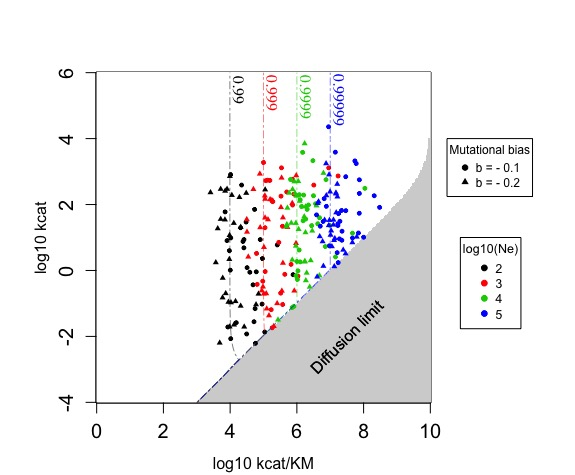
\includegraphics[scale=0.45]{Figures/2DFitLandscape_Evo_Results.jpeg}
\hspace{-1.3cm}
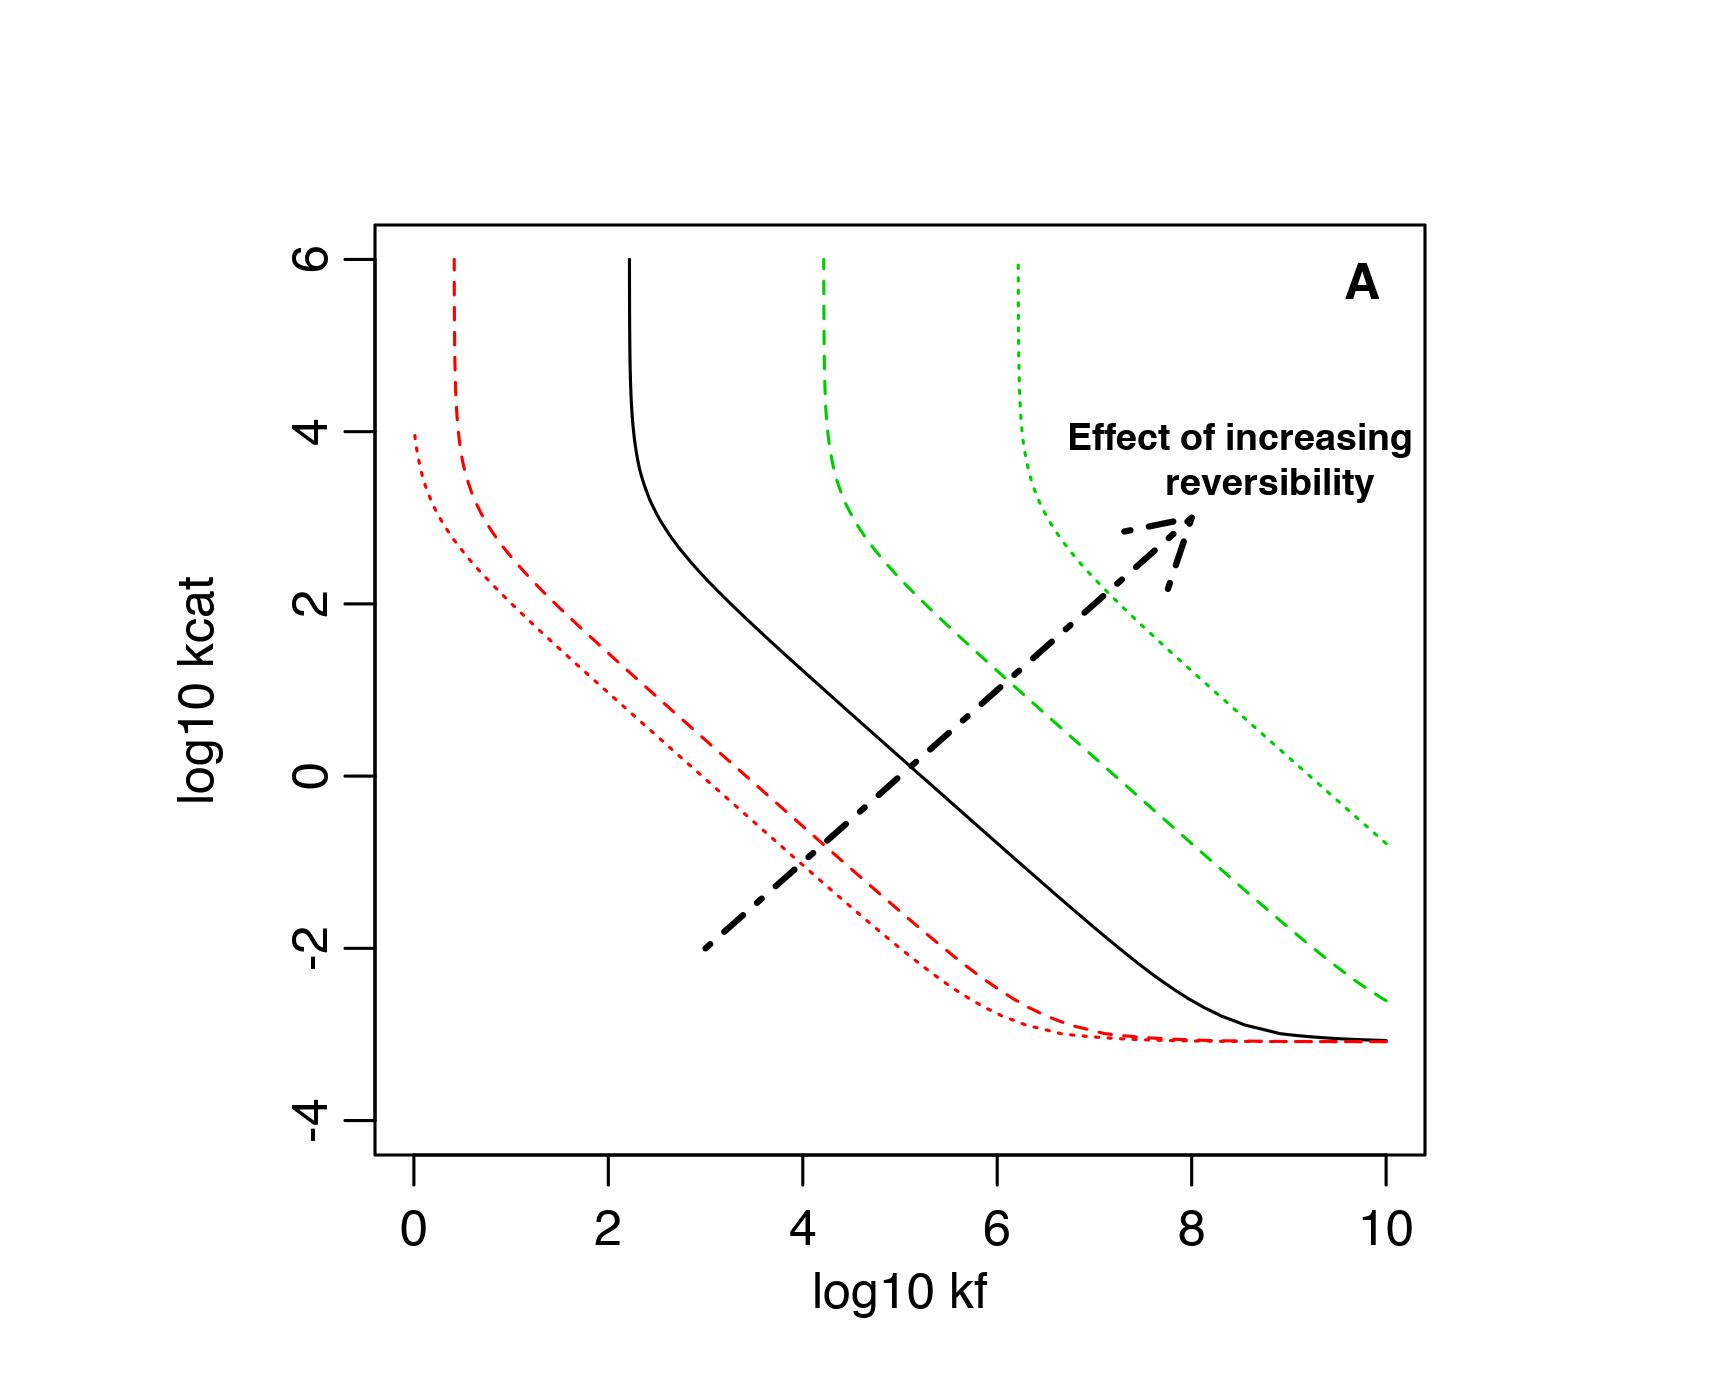
\includegraphics[scale=0.58,trim=0cm 0cm 0cm 1.5cm,clip]{pics/SM-Enzymes/2DFitLandscape_Multiple_Reverse.jpeg} 
\end{minipage} \hspace{-1.3cm}
\begin{minipage}[c]{0.49\linewidth}
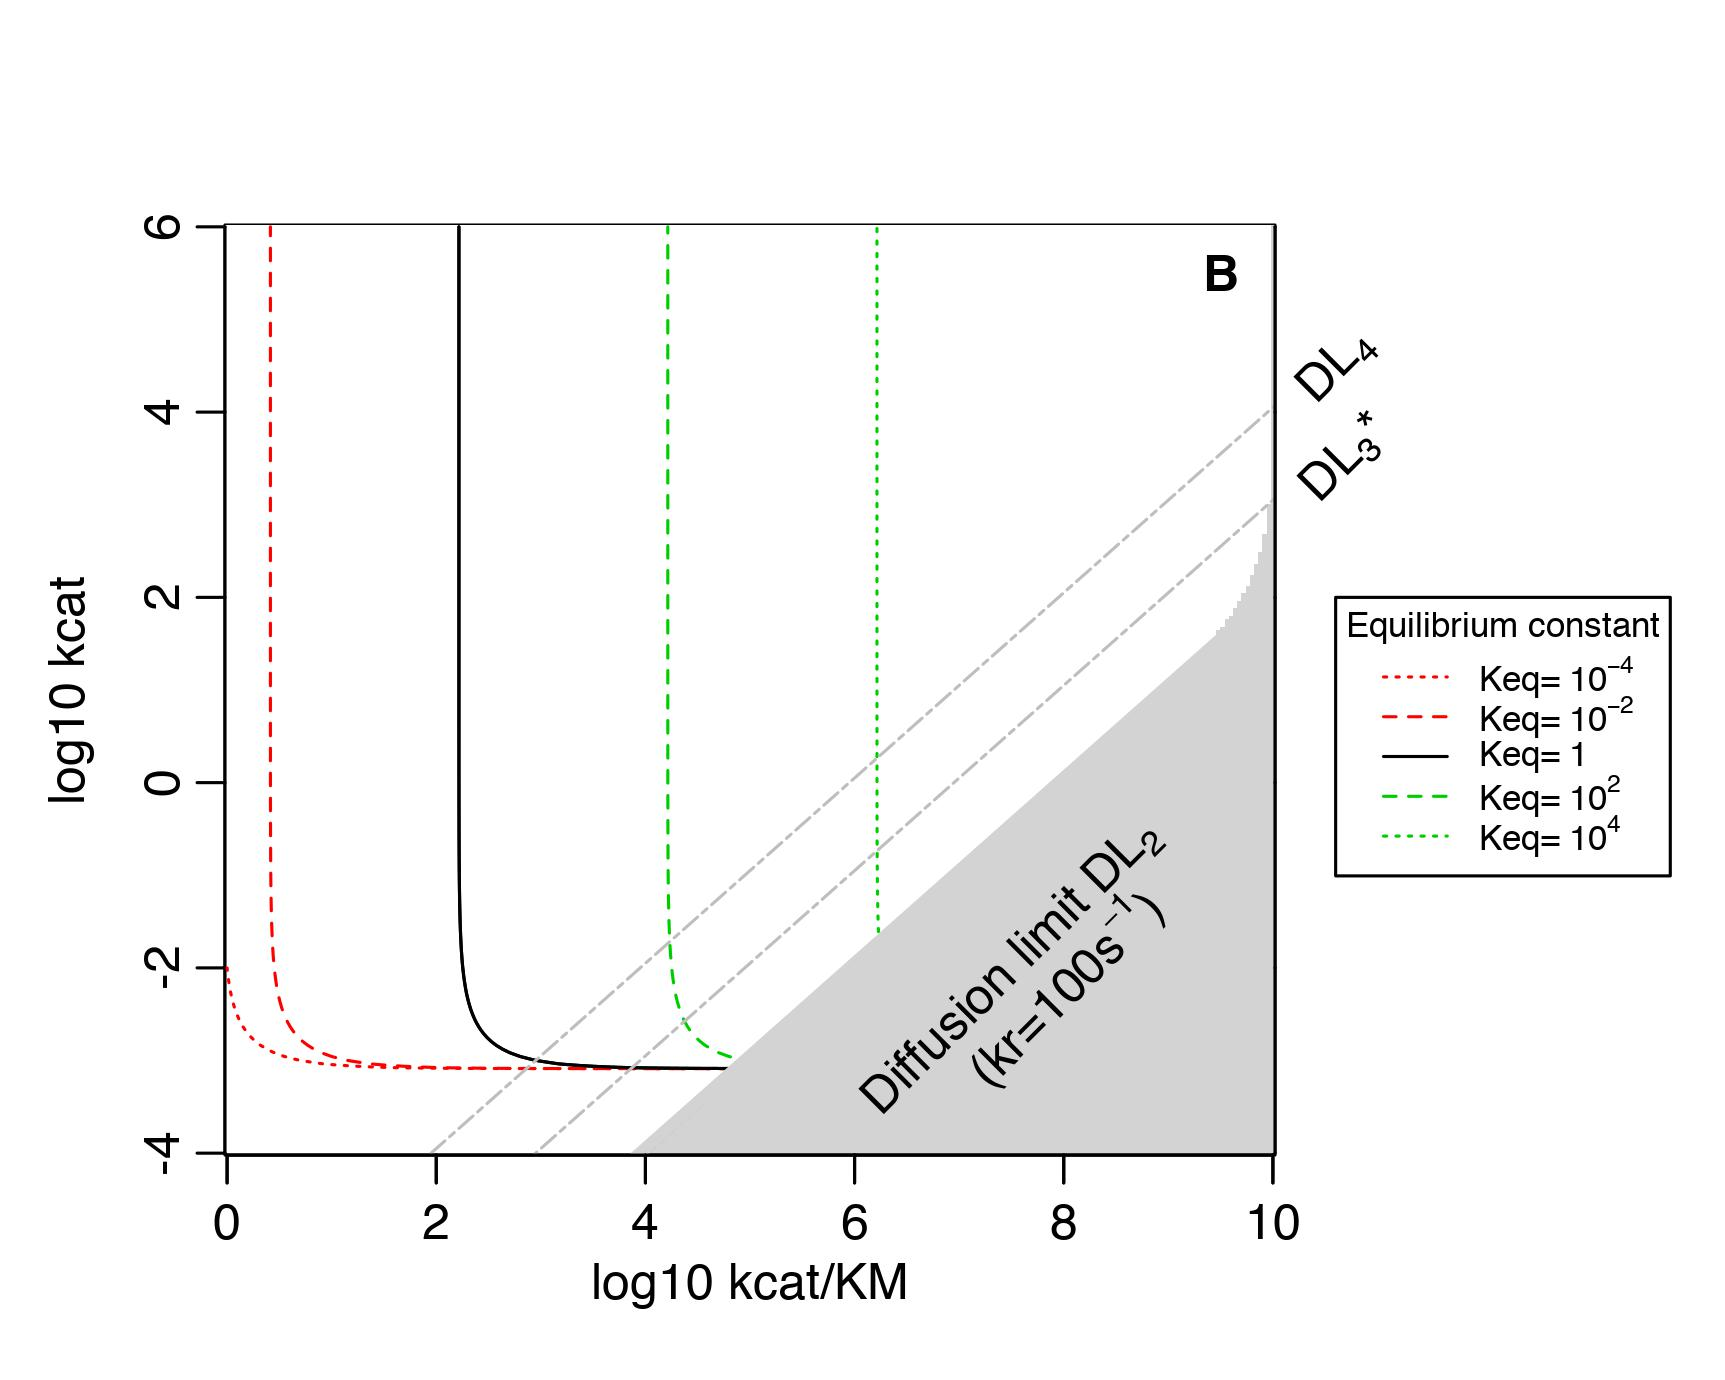
\includegraphics[scale=0.58,trim=0cm 0cm 0cm 1.5cm,clip]{pics/SM-Enzymes/2DFitLandscape_Multiple_Reverse_exp_par.jpeg}
\end{minipage}
%\vspace{0.5cm}
\caption{Backwards reaction rates of an enzyme directly upstream have a strong impact on the fitness landscape. Both plots show results of the influence of the reversibility of the first reaction on the fitness landscape of the next enzyme. Parameters are identical as in the model case for amino acids, with $k_r=10^3s^{-1}$ and $[E_{tot}]=1mM$. $K_{eq}$ equals $[S]_{eq}/[P]_{eq}=k_rk_{inh}/k_\text{cat}k_f$ \citep{Klipp94} and quantifies the degree of reversibility, a low $K_{eq}$ featuring low reversibility and vice versa. The first enzyme is a nearly perfect forward enzyme, but with $k_f=10^{8}M^{-1}$ and $k_{cat}=10^4s^{-1}$ so that we can test for enzymes being even more efficient working in reverse without using abnormal values (eg. association constant overcoming the diffusion limit set to $10^{10}M^{-1}s^{-1}$). 
%so that we can test for enzymes being even more efficient working in reverse without using abnormal values (\textit{e. g.} association constant overcoming the diffusion limit set to $10^{10}M^{-1}s^{-1}$). 
Reversibility was equally spread between the two backwards parameters (\textit{e.g.} $K_{eq}=10^2$ yields $k_r=10^{1}k_{cat}$ and $k_{inh}=10^{1}k_f$), and a low degradation rate was considered ($\eta_d=10^{-4}s^{-1}$). In (A), results are plotted in the theoretical parameter space ($k_f, \; k_\text{cat}$), showing that any increase in reversibility increases the pressure on enzyme kinetics by the same magnitude -- except when reactions are highly non-reversible (in red). In (B), the same results are shown in the experimenter parameter space of the second enzyme, showing that there is an increased pressure on $k_\text{cat}/K_M$ under higher reversibility. 
%(trivially, as the isoclines are displaced towards higher values) but also on $k_\text{cat}$, first because $k_{cat}$ and $k_{cat}/K_M$ are not independent; second, 
While the plateau is not moved upwards, indicative of a selection on $k_\text{cat}$ independent on reversibility when $k_\text{cat}/K_M$ is fixed, positive selection for this parameter may still arise due to the diffusion limit that precludes the access to the lowest $k_\text{cat}$ at high $k_\text{cat}/K_M$. The diffusion limit should play an important role for enzymes with a high dissociation rate $k_r$, as illustrated by the delineation of the diffusion limit (grey area or grey dashed lines) corresponding to several $k_r$ values (eg. DL$_3$ stands for $k_r=10^3s^{-1}$; the star indicates that it is the case represented in (A)).}
\label{figure2D_Reverse}
\end{figure*}

\begin{figure*}[h!]
\centering
\begin{minipage}[c]{0.49\linewidth}
%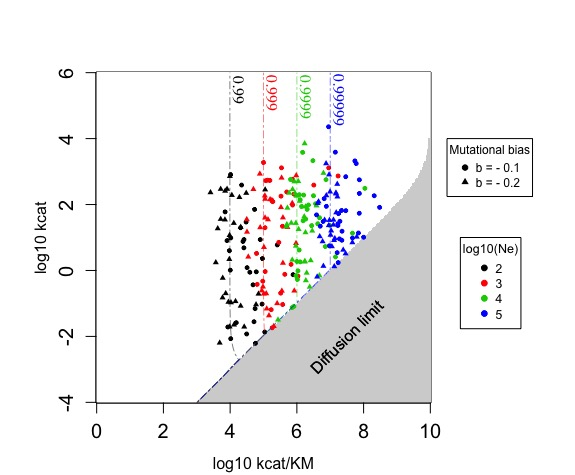
\includegraphics[scale=0.45]{Figures/2DFitLandscape_Evo_Results.jpeg}
\hspace{-1.3cm}
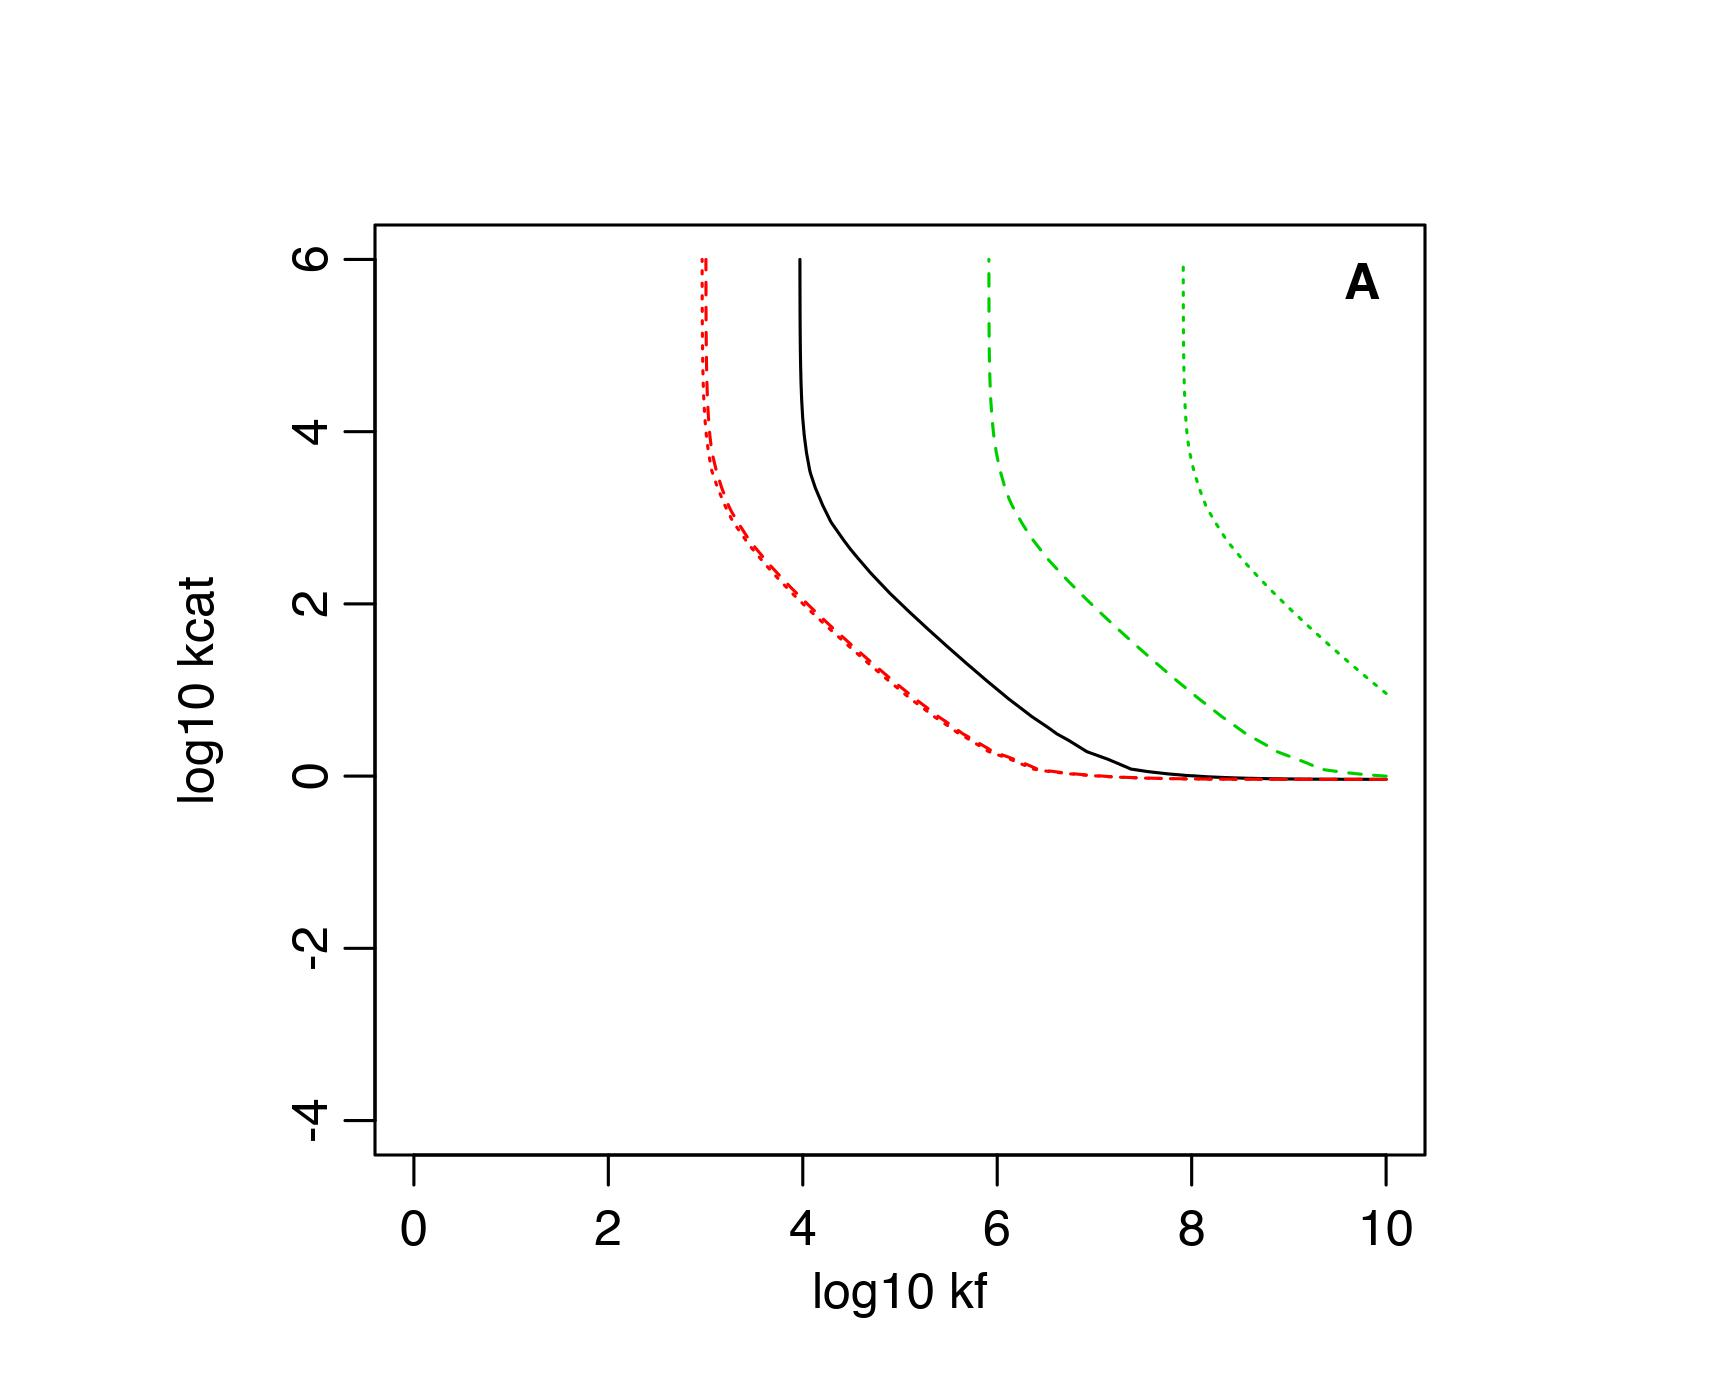
\includegraphics[scale=0.58,trim=0cm 0cm 0cm 1.5cm,clip]{pics/SM-Enzymes/2DFitLandscape_Multiple_Reverse_HighFlux.jpeg} 
\end{minipage} \hspace{-1.3cm}
\begin{minipage}[c]{0.49\linewidth}
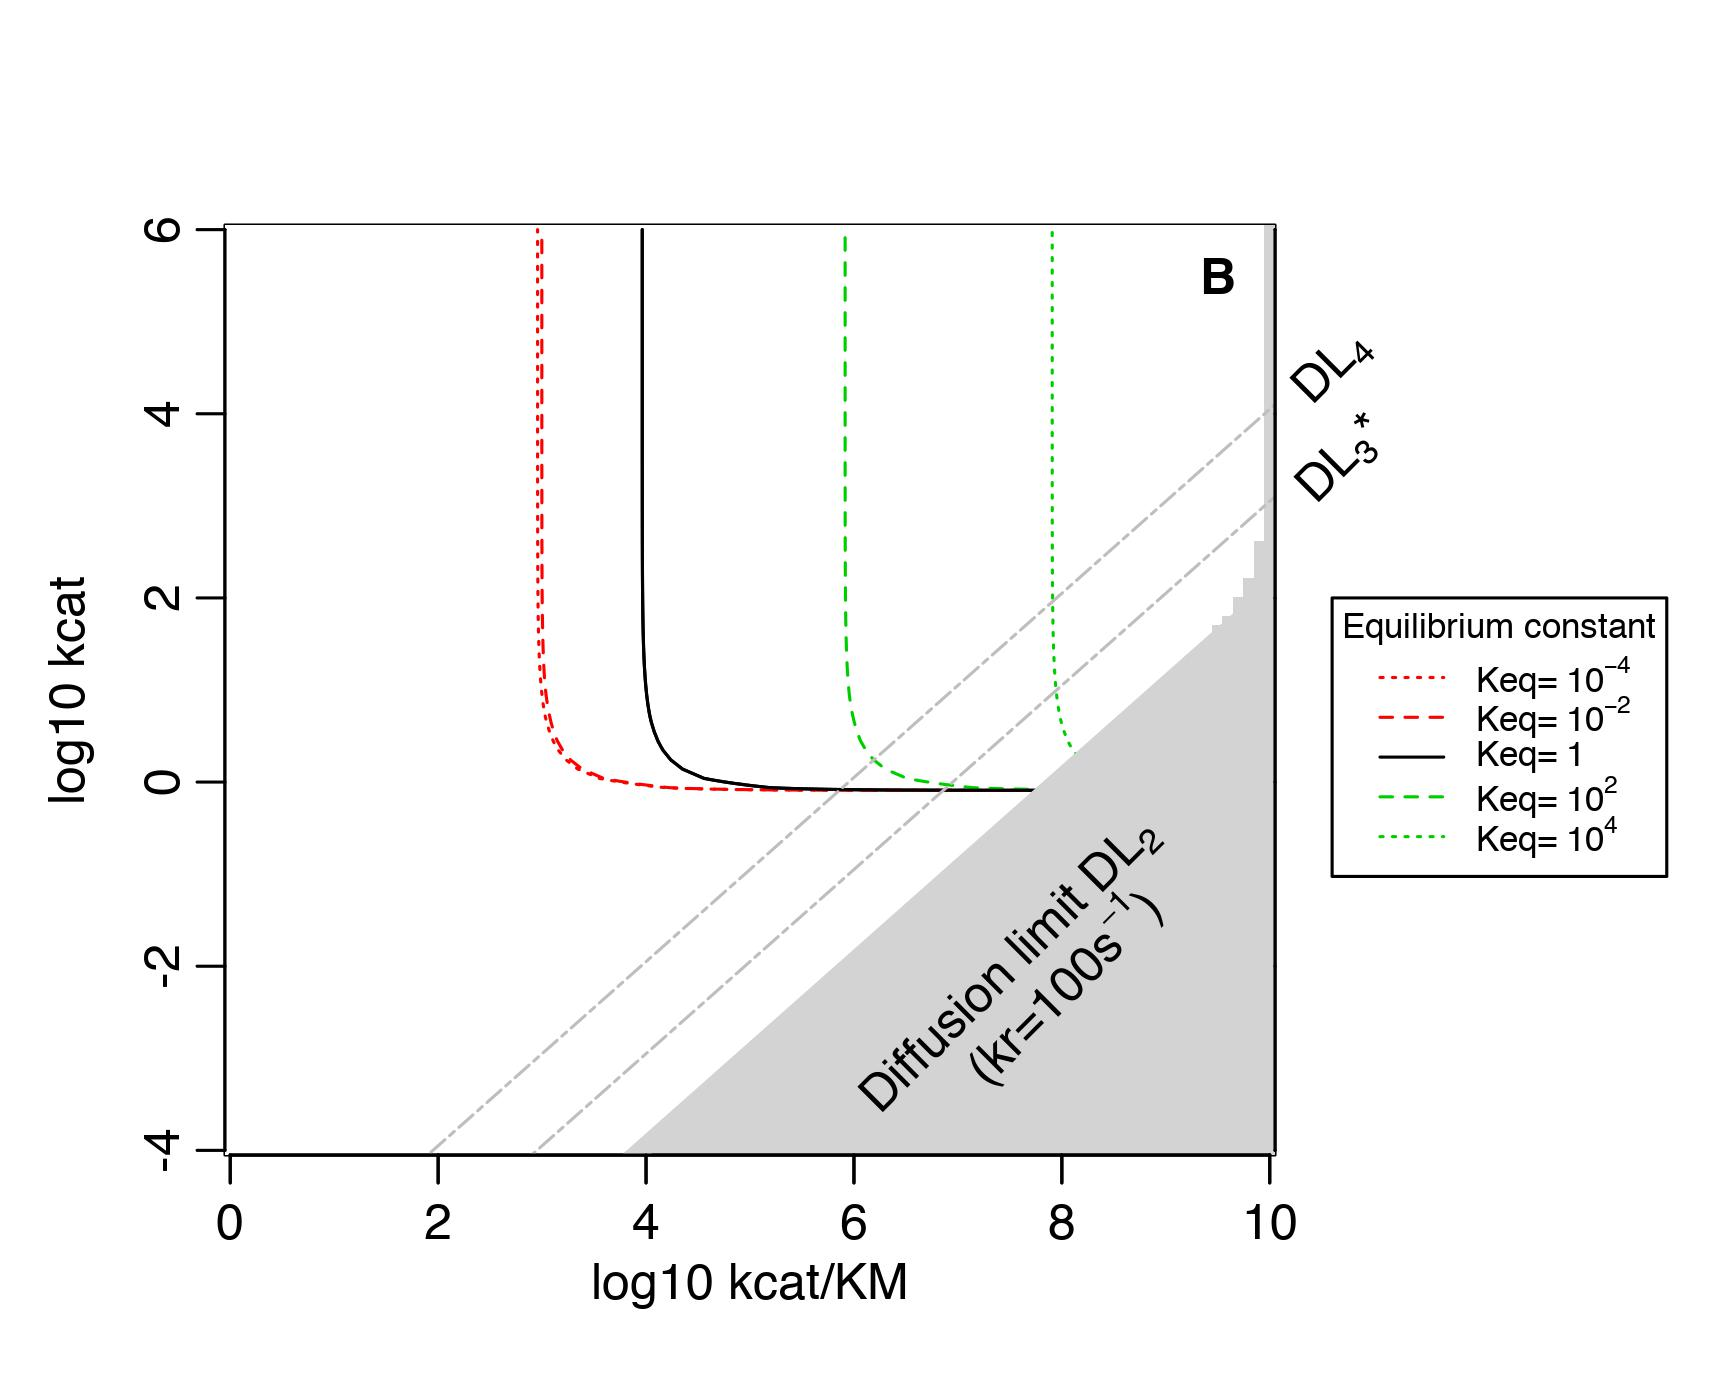
\includegraphics[scale=0.58,trim=0cm 0cm 0cm 1.5cm,clip]{pics/SM-Enzymes/2DFitLandscape_Multiple_Reverse_exp_par_HighFlux.jpeg}
\end{minipage}
%\vspace{0.5cm}
\caption{Influence of backwards parameters on fitness landscapes: both plots show results of the influence of the reversibility of the first reaction on the fitness landscape of the following enzyme. Parameters for uptake are $V_{Tm}=1mM.s^{-1}$ and $K_T=5mM$, corresponding to the model case for sugars. The settings for enzymes are also the same as the generic ones used previously (highly concentrated enzymes and $k_r=10^3s^{-1}$).%$K_{eq}$ equals $[S]_{eq}/[P]_{eq}=k_rk_{inh}/k_{cat}k_f$ \citep{Klipp94} and quantifies the degree of reversibility - low $K_{eq}$ featuring low reversibility and vice versa.
The first enzyme is a nearly perfect forward enzyme, but with $k_f=10^{8}M^{-1}$ and $k_{cat}=10^4s^{-1}$. Reversibility was equally spread between the two backwards parameters (eg. $K_{eq}=10^2$ yields $k_r=10^{1}k_{cat}$ and $k_{inh}=10^{1}k_f$), and a low degradation rate was considered ($\eta_d=10^{-4}s^{-1}$). In (A), results are plotted in the theoretical parameter space (made up of $k_f$ and $k_{cat}$), showing that any increase in reversibility increases the pressure on enzyme kinetics by the same magnitude -- except when reactions are highly irreversible (in red) -- because the first product, instead of accumulating, may thus often react backwards and limit the flow progressing forward. In (B), the same results are shown in the experimenter parameter space of the second enzyme, showing that there is an increased pressure on $k_{cat}/K_M$ (trivially, as the isoclines are displaced towards higher values) but also on $k_{cat}$, first because $k_{cat}$ and $k_{cat}/K_M$ are not independent; second, because the diffusion limit precludes the access to high $k_{cat}/K_M$ for a wider range of $k_{cat}$ values when the pressure on $k_{cat}/K_M$ is higher. This is particularly true when the dissociation rate $k_r$ of the second enzyme is high, as illustrated by the delineation of the diffusion limit (grey area or grey two-dashed lines) corresponding to several $k_r$ values.}
\label{fig8-ann}
\end{figure*}

%As stated in the main manuscript, reversibility is an intrinsic feature of chemical reactions that cannot be directly overcome by Evolution \citep{Haldane30,Cornish-Bowden79a}. A highly reversible reaction corresponds to a large intrinsic equilibrium constant $K_{eq}=[S]_{eq}/[P]_{eq}$ \citep{Klipp94}, and results in higher backward than forward rates in the following chemical equation: \begin{equation}
%\ce{ E + S <=>[k_{f}][k_{r}] ES <=>[k_{cat}][k_{inh}] E + P_1 },
%\label{chemMM_fullrev}
%\end{equation}
%where $k_{inh}$ represents the rate at which enzyme and product combine back. Such a (reversible) reaction could in principle influence the selective pressure acting on the following enzyme in the pathway, for both enzymes compete to process the same metabolite $P_1$. We thus quantified how reversibility affects the evolution of an enzyme downstream (Figure~\ref{figure2D_Reverse} ; using the same model case parameters used throughout the paper (see FIG.1 of the paper
%for details) and considering a nearly perfect first enzyme for consistency: $k_{cat}=10^4s^{-1}$,$k_f=10^8M^{-1}s^{-1}$).% to avoid outliers for backward parameters (see legend of Fig.~\ref{figure2D_Reverse} for details on how we distributed the effect of reversibility among parameters)
%We also estimated the impact of the dissociation constant of the second reaction on the fitness landscape. To begin, both enzymes are still highly concentrated ($[E]_{tot}=1mM$), an evolvable quantity whose well-documented effect is eventually assessed at the end of the section.

Discussion of the direct effect of reversibility can be found in the dedicated section of the paper while 
% (FIG.~\ref{figure2D_Reverse}-A). Indeed, increasing $K_{eq}$ moves the fitness plateau toward the upper-right corner in the ($k_f$,$k_\text{cat}$) parameter space, hence selecting for more efficient downstream enzymes. The effect appears linear, except for very low values of $K_{eq}$ where it fades -- such that a 100-fold change in $K_{eq}$ has little impact -- because the main issue when reactions are highly non-reversible becomes, again, metabolite accumulation. Therefore, the reversibility of the upstream reaction appears like a critical parameter for the evolution of an enzyme, able to generate large changes in evolutionarily expected kinetic parameters.
the graphical results on which this dicussion is based are presented in Figures \ref{figure2D_Reverse} for a low flux and \ref{fig8-ann} for a high flux. Both of them are shown in the theoretical's (A) and experimenter's (B) parameter space to better grasp how basic properties give rise to phenomenological ones. Overall, the equilibrium constant $K_{eq}$ has a rather similar impact on the fitness landscape of the next enzyme than the non-linear toxicity function, with a highly reversible upstream enzyme exerting a selection pressure downstream towards an increase of kinetic parameters.

\begin{figure*}[h!]
\centering
\begin{minipage}[c]{0.49\linewidth}
%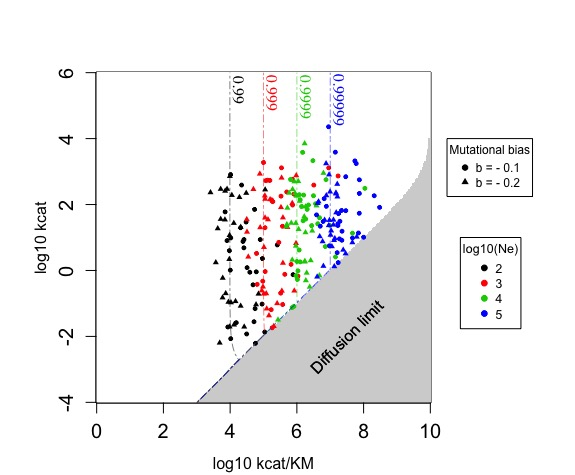
\includegraphics[scale=0.45]{Figures/2DFitLandscape_Evo_Results.jpeg}
\hspace{0cm}
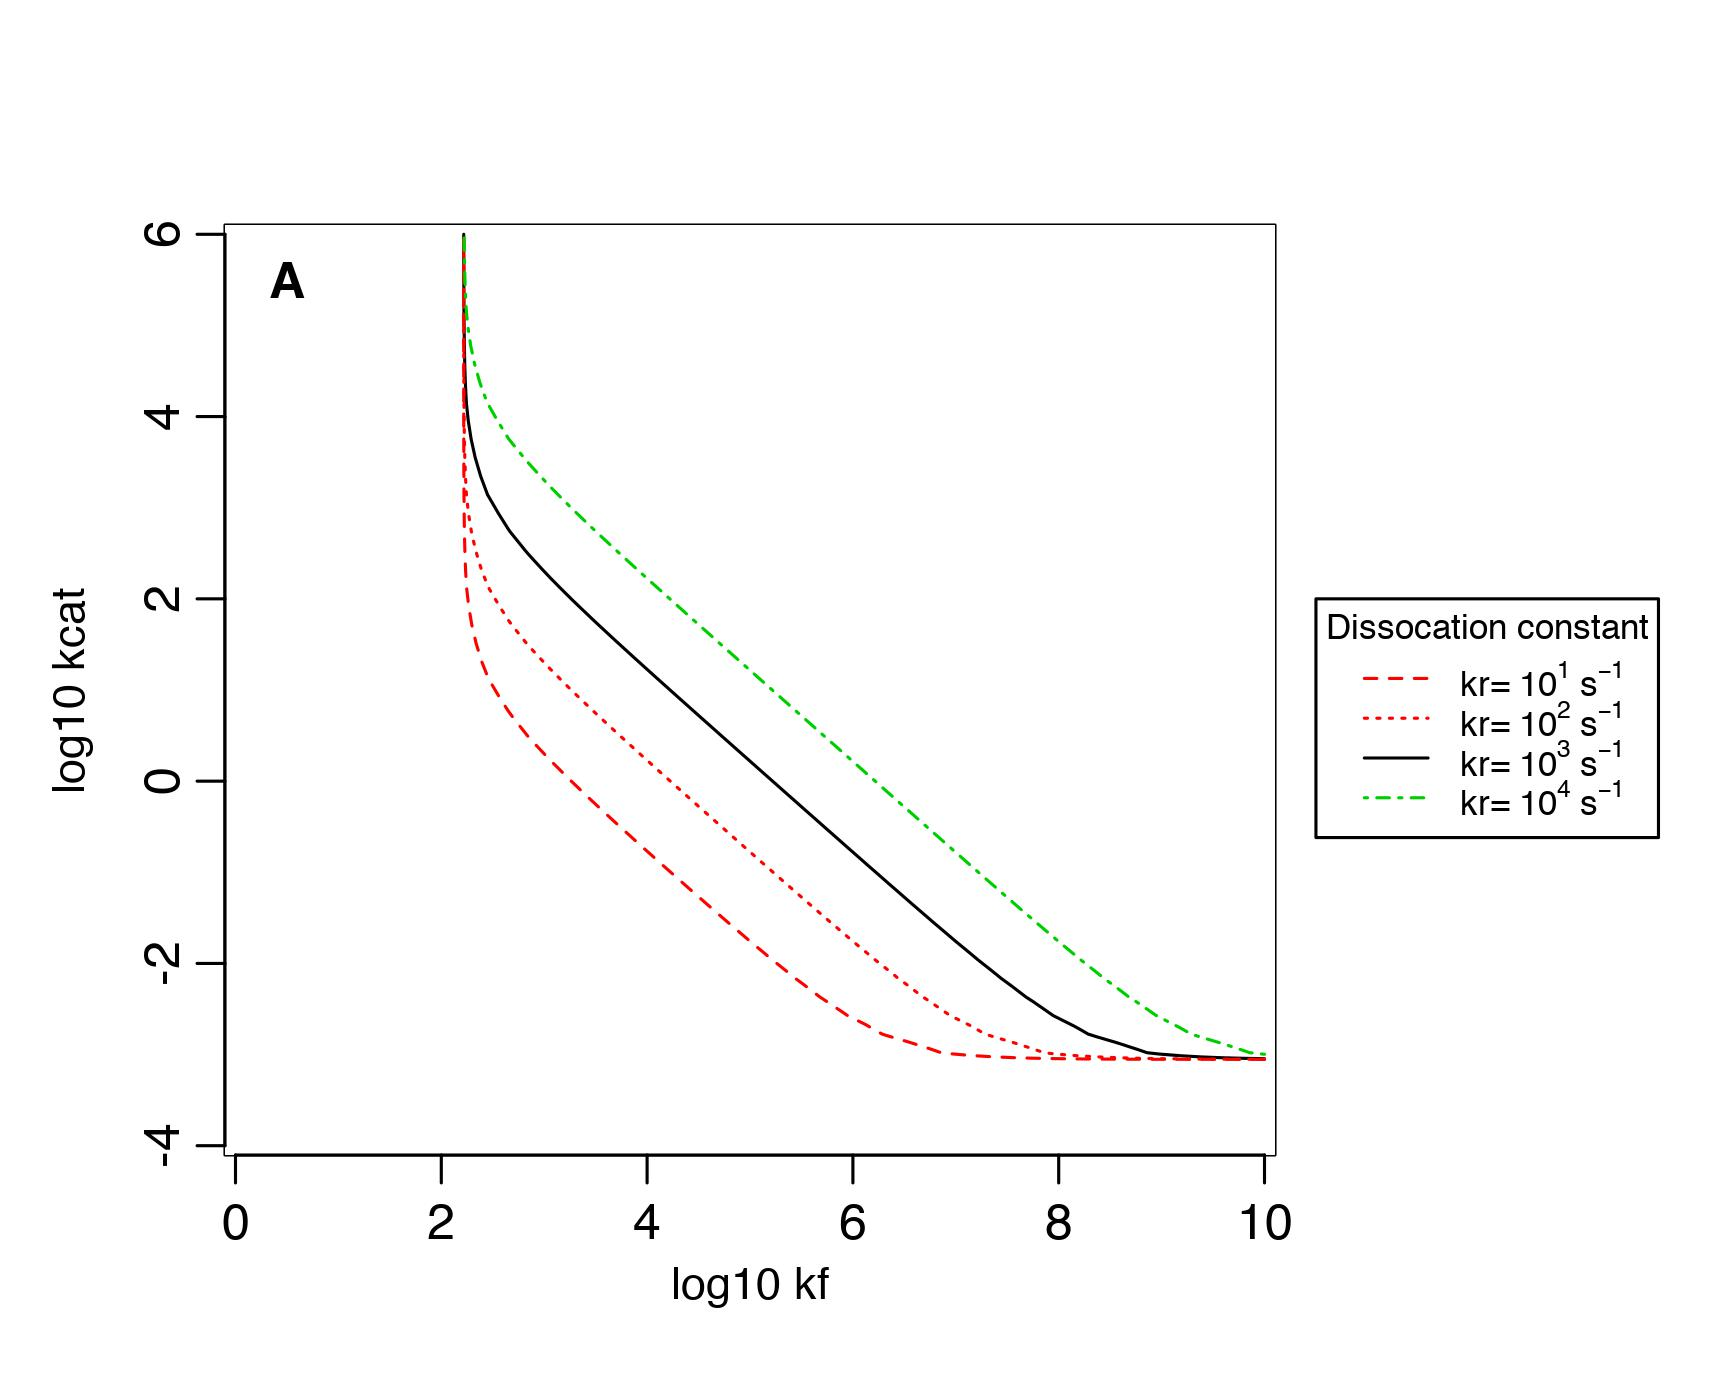
\includegraphics[scale=0.54,trim=0cm 0cm 0cm 1.5cm,clip]{pics/SM-Enzymes/2DFitLandscape_kr_sens.jpeg} 
\end{minipage} \hspace{0cm}
\begin{minipage}[c]{0.49\linewidth}
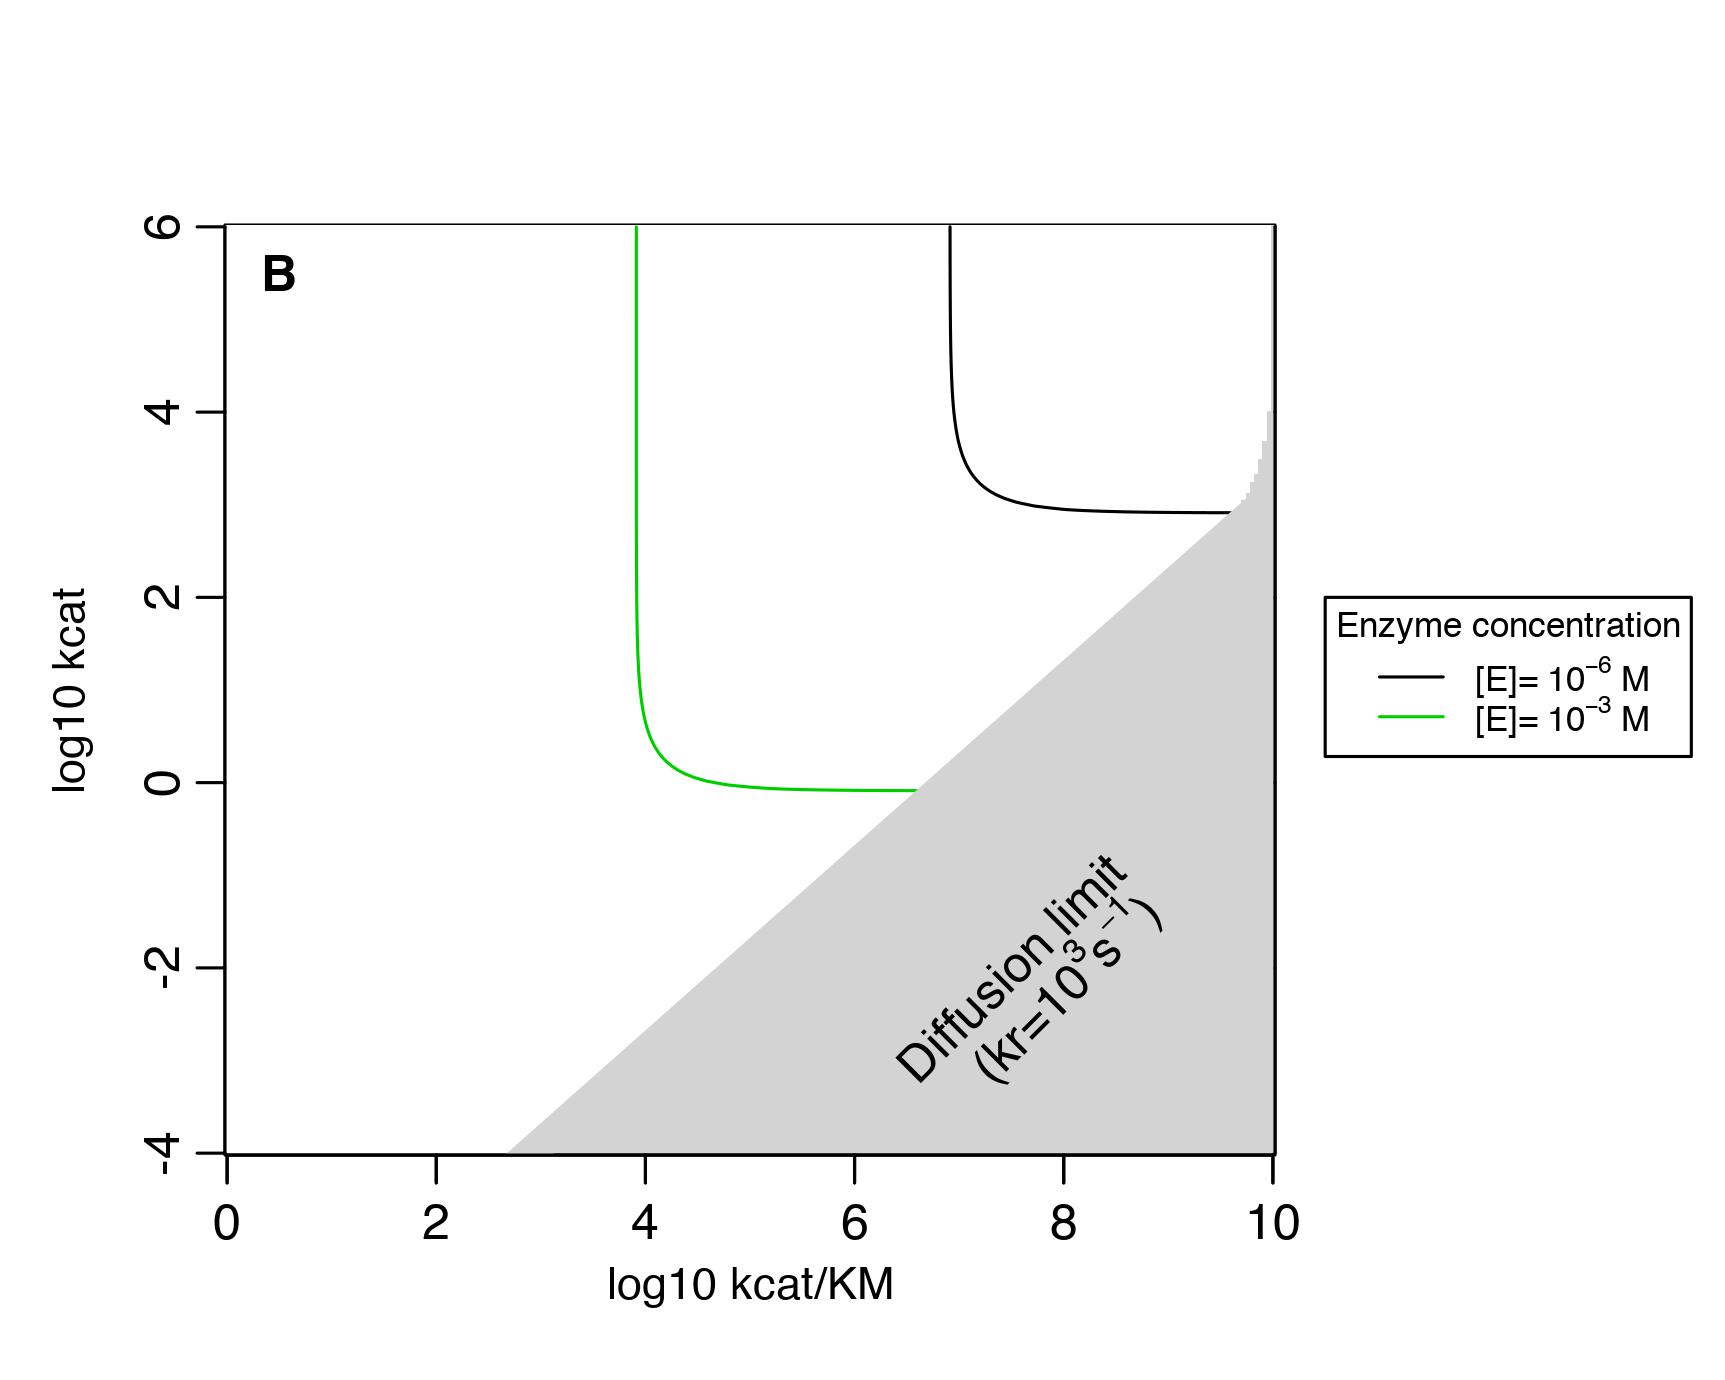
\includegraphics[scale=0.54,trim=0cm 0cm 0cm 1.5cm,clip]{pics/SM-Enzymes/Plot2DFitLandscape_Enz_conc_HighFlux.jpeg}
\end{minipage}
%\vspace{0.5cm}
\caption{Influence of several kinetic quantities involved in catalytic activity. (A) Influence of the dissociation constant $k_r$ on the joint selective pressure acting on forward parameters $k_{cat}$ and $k_f$ for the model case of the first enzymes involved in the processing of amino acids (see FIG. 1 in main body of article). (B) Influence of enzyme concentration on the pressure acting on forward parameters in the model case for sugars ($V_{Tm}=1mM.s^{-1}$ and $K_T=1mM$): see next figure for the effect in the context of amino acids-like pathways, coupled to the influence of reversibility. In this panel, increasing an enzyme concentration is not costly, which is an unrealistic assumption relaxed later.}
\label{fig9-ann}
\end{figure*}

Increasing reversibility through an increase in $k_r$ (Figure \ref{fig9-ann}-A) increases the selective pressure on both kinetic parameters downstream -- except for very low $k_r$ -- jointly pushing them towards higher values. %, thereby increasing $k_{cat}/K_M$ without getting stuck by the diffusion limit. 
%Moreover, as $k_r$ increases, the negative relationship between $k_\text{cat}$ and $k_f$ (on a part of the fitness landscape isocline) is enhanced; in other words, increasing $k_r$ makes the two other kinetic parameters more interchangeable.
When using the ``empirical" parameter space (Figure~\ref{figure2D_Reverse}-B), we observe that increasing reversibility $K_{eq}$ only selects for higher $k_\text{cat}/K_M$ in principle. Yet, the diffusion limit constraint also matters since it removes accessibility to the high $k_{cat}/K_M$, low $k_{cat}$ part of the landscape (see grey area and grey lines on Figure~\ref{figure2D_Reverse}-B). As $K_{eq}$ sets the ratio between the four kinetic parameters, the joint evolution of forward and backward rates is determined by the dependency this ratio creates : indeed, higher reversibility comes on average with higher $k_r$s for similar turn-over rates $k_{cat}$, which means that higher reversibility pushes both $k_{cat}$ and $k_{cat}/K_M$ to the upper right corner. On the contrary, when $K_{eq}$ is low, the diffusion limit may vanish from the experimenter's space and opens it up completely. As a consequence, the unbinding rate $k_r$ of an enzyme may eventually fuel a positive codependency between the forward rates $k_\text{cat}$ and $k_f$ as the latter is no longer sufficient to ensure a high $k_\text{cat}/K_M$ (see Figure~\ref{figure2D_Reverse}-B and Figure~\ref{fig8-ann}-B of SM for this influence in the theoretical parameter space).

Because optimal concentrations may generally be below $10^{-3}M$ and since the flux is determinant in the drawing of the fitness landscape (especially when accounting for toxicity of metabolites), the influence of epistasis between following enzymes also differs (see Figure \ref{fig11bis-ann}). This means that when toxicity is the main driver of the selective pressure, the moderate epistasis - between kinetic parameters of neighbouring enzymes - shown with high concentrations (see Figure \ref{fig4c-ann}) increases if lower concentrations are assumed.

\begin{figure*}[h!]
\vspace{-0.75cm}
\centering
\begin{minipage}[c]{0.49\linewidth}
%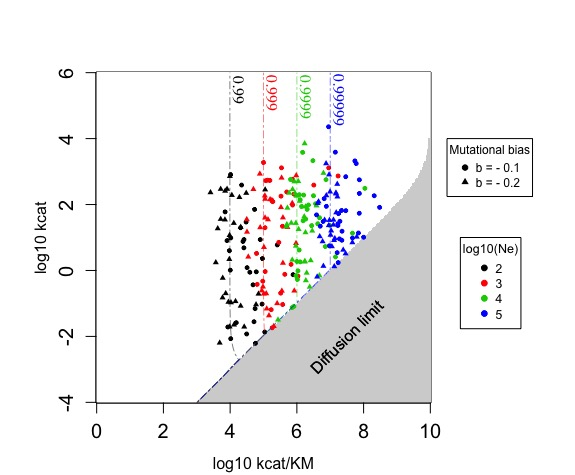
\includegraphics[scale=0.45]{Figures/2DFitLandscape_Evo_Results.jpeg}
\hspace{-0.5cm}
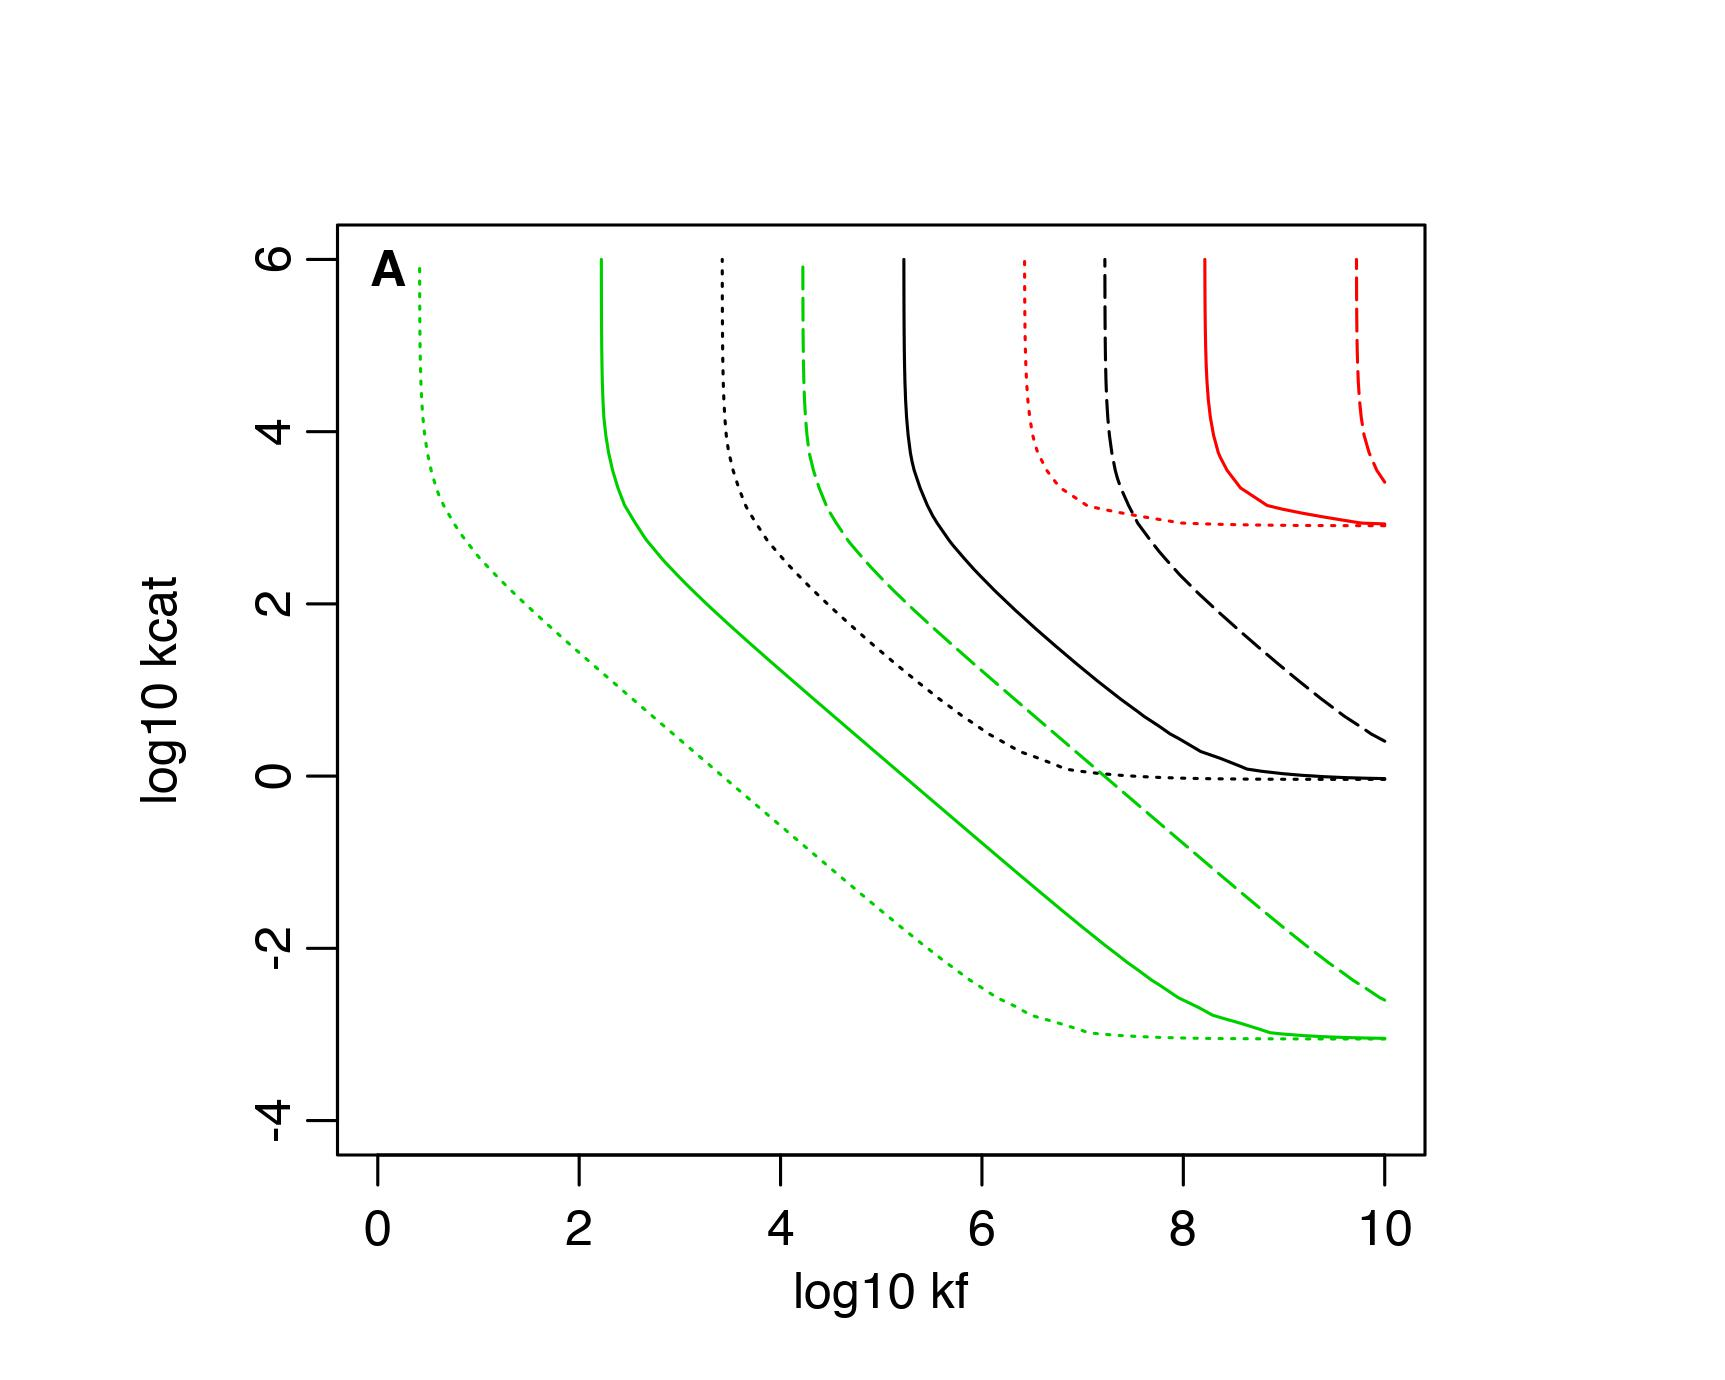
\includegraphics[scale=0.52,trim=0cm 0cm 0cm 1cm,clip]{pics/SM-Enzymes/Fit_Econc_sens2Enz.jpeg} 
\end{minipage} \hspace{-1cm}
\begin{minipage}[c]{0.49\linewidth}
\includegraphics[scale=0.52,trim=0cm 0cm 0cm 1cm,clip]{pics/SM-Enzymes/Fit_Econc_sens2Enz_kactKM.jpeg}
\end{minipage}
%\vspace{0.5cm}
\caption{Influence of enzyme concentration on kinetic parameters for the model case of amino acids ($V_{Tm}=1\mu M.s^{-1}$ and $K_T=50\mu M$) followed by a nearly perfect enzyme and including a low degradation rate ($\eta_d=10^{-4}s^{-1}$) for the first product, represented in (A) the theroretical parameter space; and (B) the experimenter's parameter space: the case of downstream enzymes in a pathway. These plots show the joint variability introduced by the reversibility of the previous -- the first one here -- reaction and the concentration of the enzyme of the focal -- the second one here -- reaction. General trends are identical than for the first enzyme and reversibility of the previous reaction has the same effect (with the same magnitude) no matter the enzyme concentration. Decreasing enzyme concentration pushes the fitness plateau towards higher values of both $k_{cat}$, $k_f$ and $k_{cat}/K_M$. In this panel, increasing an enzyme concentration is not costly, which is an unrealistic assumption relaxed later.}
\label{fig10-ann}
\end{figure*}

\begin{figure*}[h!]
\vspace{-0.5cm}
\centering
%\begin{minipage}[c]{0.48\linewidth}
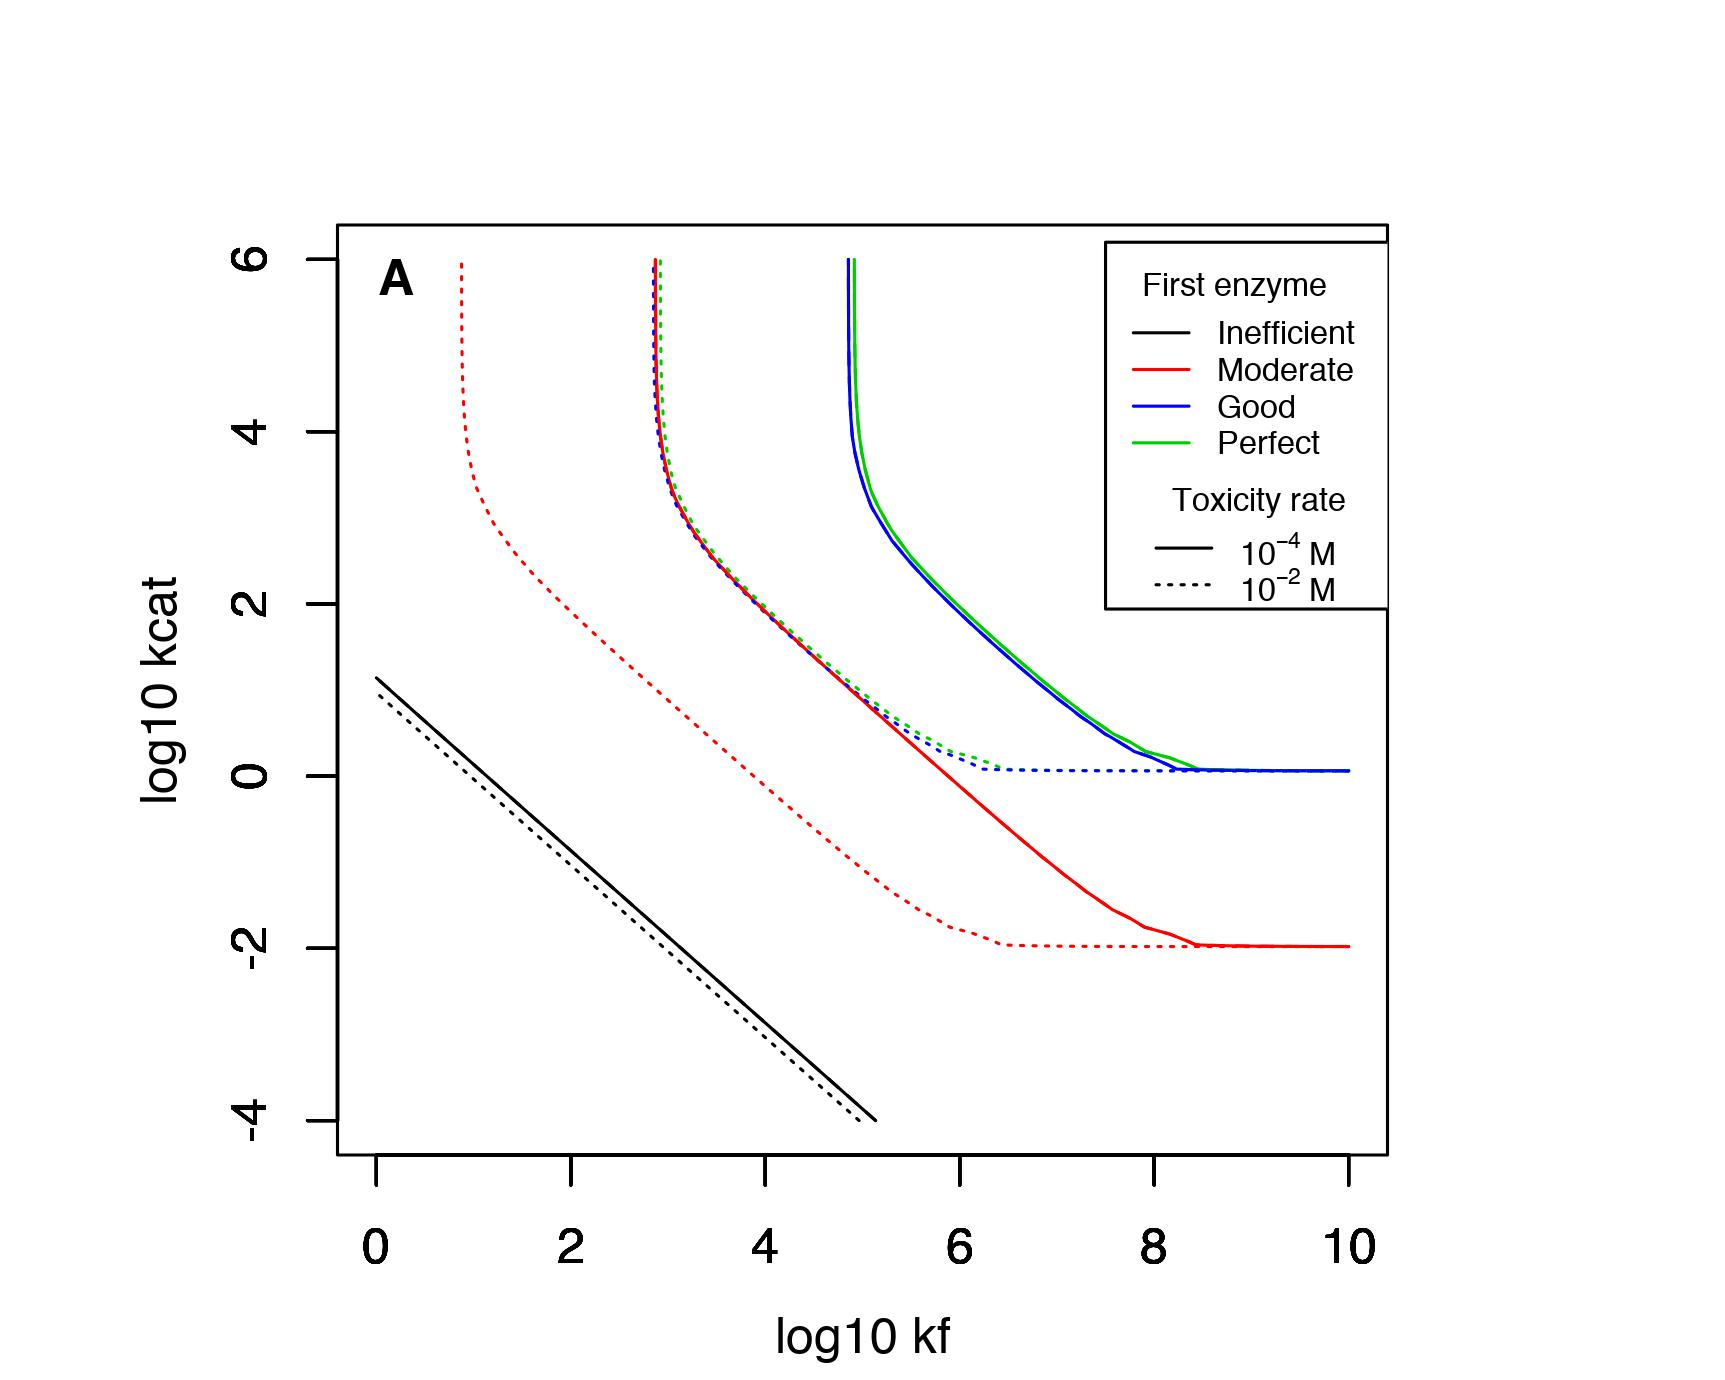
\includegraphics[scale=0.54,trim=0cm 0cm 0cm 0.5cm,clip]{pics/SM-Enzymes/2DFit_Landscape_2Enz_First_Enz_Influence&Tox&DegLow&Conc_Low.jpeg} 
\hspace{-0.5cm}
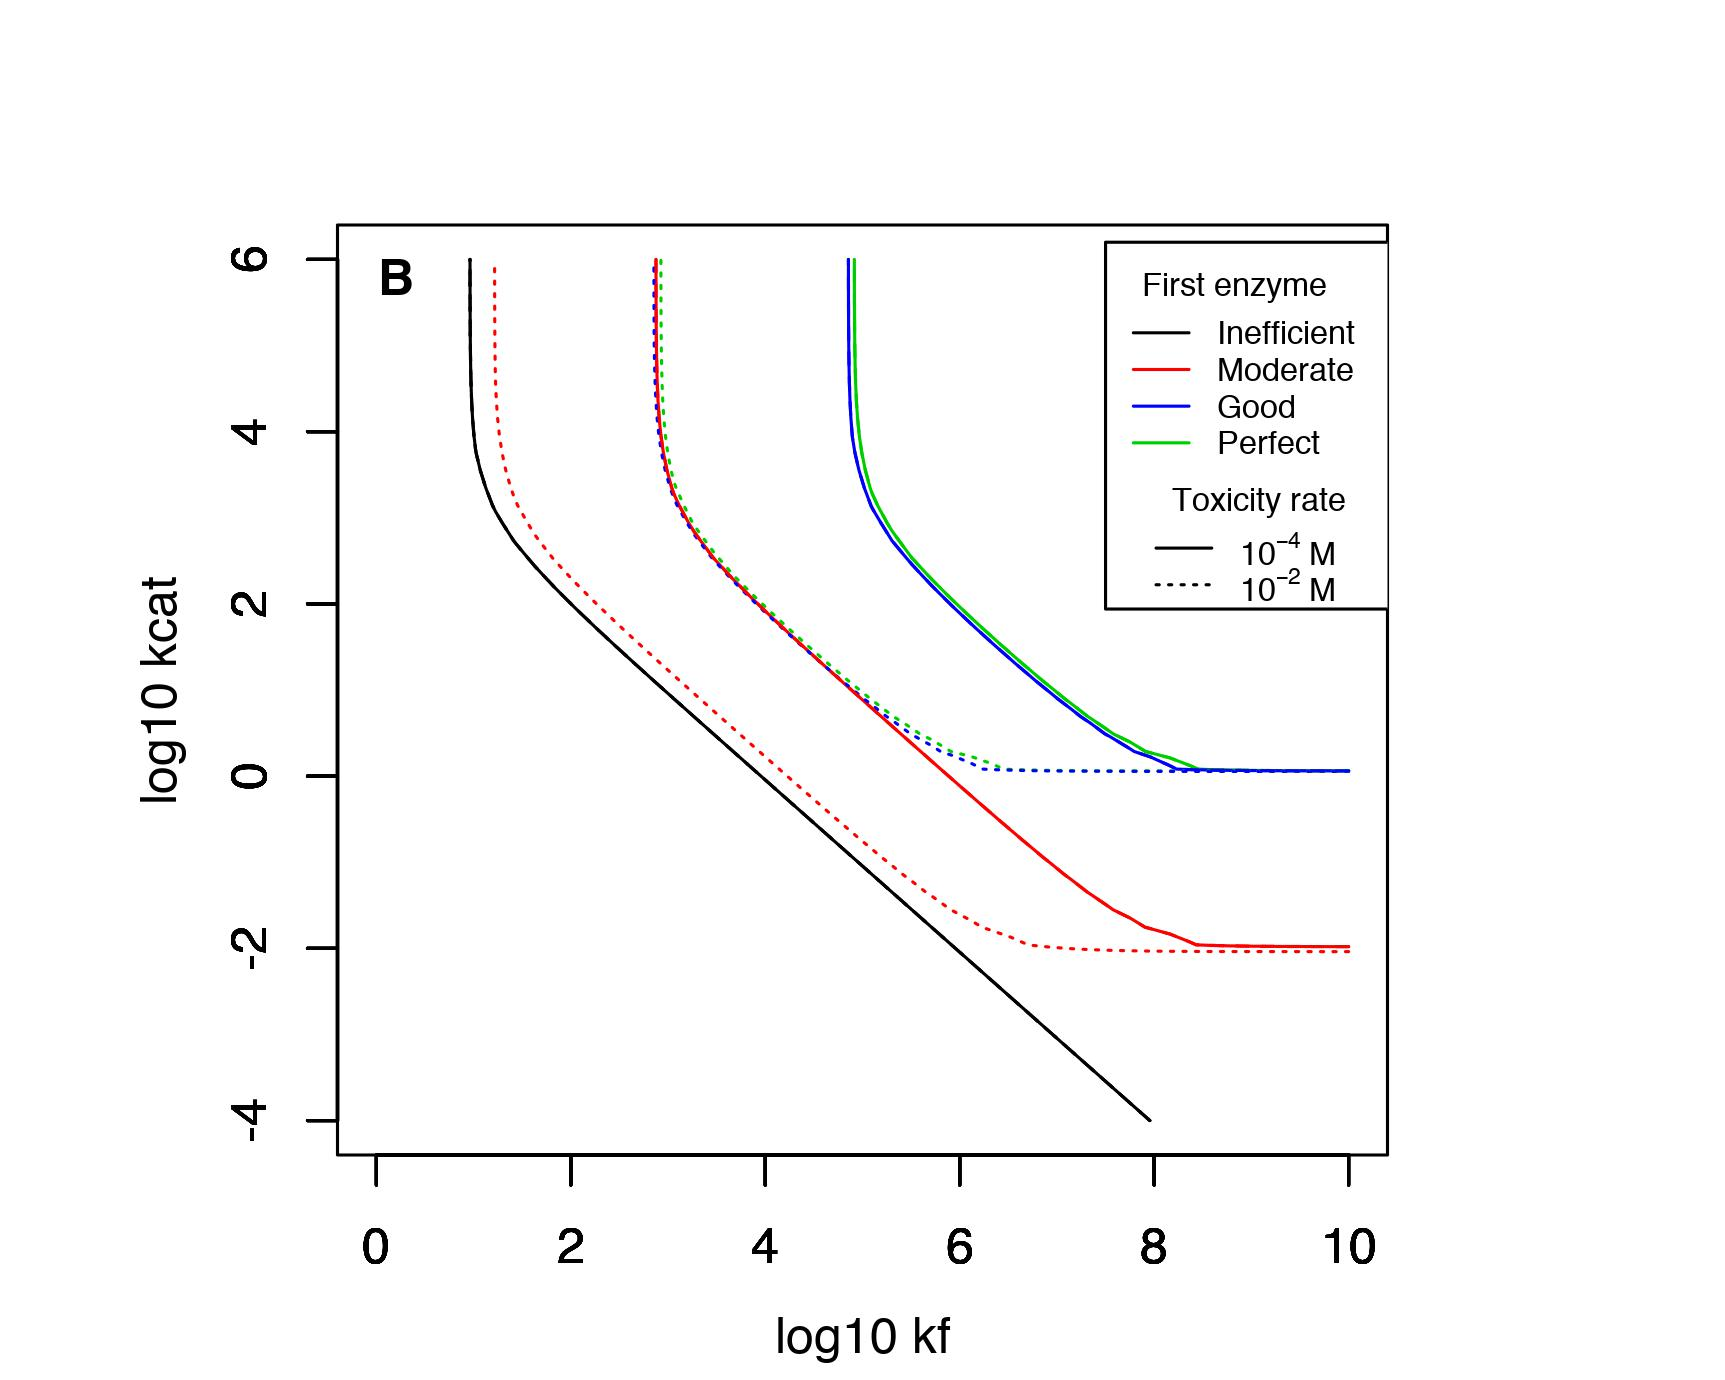
\includegraphics[scale=0.54,trim=0cm 0cm 0cm 0.5cm,clip]{pics/SM-Enzymes/2DFit_Landscape_2Enz_First_Enz_Influence&Tox&DegMod&Conc.jpeg}
%\end{minipage} \hspace{-1cm}
%\begin{minipage}[c]{0.48\linewidth}
%\includegraphics[scale=0.5,trim=0cm 0cm 0cm 1.5cm,clip]{Figures/Fit_Econc_sens2Enz_kactKM.jpeg}
%\end{minipage}
%\vspace{0.5cm}
\caption{Influence of the first enzyme efficiency on the landscape of a second enzyme involved in the same pathway, considering two different levels of toxicity along a low degradation rate ($\eta_d=10^{-6}s^{-1}$) in (A) and a moderate one ($\eta_d=10^{-2}s^{-1}$) in (B). Contrary to preceding figures, the concentration is now set to $[E_{tot}]=1\mu M$ to see how it may influence epistasis relationships within a pathway. Four first enzyme efficiencies are considered (Inefficient : $k_f=10^2M^{-1}.s^{-1}$, $k_{cat}=10^{-2}s^{-1}$; Moderate : $k_f=10^5M^{-1}.s^{-1}$, $k_{cat}=10^{2}s^{-1}$; High : $k_f=10^7M^{-1}.s^{-1}$, $k_{cat}=10^{4}s^{-1}$ ; Perfect : $k_f=10^{10}M^{-1}.s^{-1}$, $k_{cat}=10^{6}s^{-1}$). We see here, that toxicity being a major factor of influence, it changes how the fitness landscape of a second enzyme reacts to different first enzyme efficiencies. This is expected since toxicity dependent lanscapes have been proved to be sensitive to the level of flux. In (B), an inefficient enzyme is more constrained because the higher degradation rate still competes with the second enzyme at relatively low metabolite concentrations.}
\label{fig11bis-ann}
\end{figure*}

\noindent\paragraph{Enzyme concentration and shape of the fitness landscape}

\begin{figure*}[h!]
\centering
%\begin{minipage}[c]{0.48\linewidth}
%\includegraphics[scale=0.45]{Figures/2DFitLandscape_Evo_Results.jpeg}
\hspace{-0.5cm}
\includegraphics[scale=0.6,trim=0cm 0cm 0cm 0cm,clip]{pics/SM-Enzymes/1DFit_Lanscape_Scaling_Concentration.jpeg} 
%\end{minipage} \hspace{-1cm}
%\begin{minipage}[c]{0.48\linewidth}
%\includegraphics[scale=0.5,trim=0cm 0cm 0cm 1.5cm,clip]{Figures/Fit_Econc_sens2Enz_kactKM.jpeg}
%\end{minipage}
%\vspace{0.5cm}
\caption{Influence of enzyme concentration on the fitness landscapes for different combinations of enzyme kinetic parameters and different costs of production. The panels represent the absolute value of the $log_{10}$ spread between the maximum fitness and the fitness for the concentration represented on the x-axis, such that a peak corresponds to high fitness. $k_{cat}$ improves from left to right (specific values indicated at the top of each column) and $k_f$ improves from top to bottom (specific values indicated at the right of each row). The grey area delimits the crowding limit where fitness equals zero because the cytoplasm undergoes the glass transition; obviously, because diffusion slows down before reaching this level, fitness starts to plummet for concentrations approximately an order of magnitude below (see the case of a moderately low $k_f$ on the first row, where the cost of expression is not the dominant constraint). In parallel, the protein cost exerts a linear influence with expression, which is especially important when kinetic parameters are higher, as outlined by the cost-dependent spread of the influence of concentration in the lower panels. This means that Natural Selection should oppose the protein burden differently for protein of different costs and that drift should in turn act differently upon enzyme kinetic parameters depending on the values of $N_e$s since the burden differs with these parameters.}
\label{fig11-ann}
\end{figure*}

Finally, levels of gene expression can also influence an enzyme's catalytic activity, and as such, high enzyme concentrations can relax the selective pressure acting on enzyme kinetic parameters, whereas very low concentrations require that extreme kinetic efficiencies evolve when the metabolic demand is high like in the case for sugars (see Figure \ref{fig9-ann}B). In this context, the influence of enzyme concentrations is similar for the second enzyme (see Figure \ref{fig10-ann}) such that increasing it comes with a relaxed selective pressure on both $k_\text{cat}$ and $k_f$ (and $k_\text{cat}/K_M$). %Here again, we see that increasing the specificity constant $k_\text{cat}/K_M$ may have no influence on the flux due to the dependency of the latter on both kinetic parameters in some parts of the parameter space% (especially true when there is a discrepancy between efficiency of binding and turn-over)

However, we have unreasonably assumed here that gene expression is cost-free, an assumption that we now relax by introducing two well documented costs: 1) the cost of protein production and 2) the cost of (excessive) macromolecular crowding. Therefore, on the one hand $[E_{tot}]$ increases the flux by increasing the enzyme kinetic activity while on the other hand, it hinders diffusion in an exponential manner and reduces the net effect of flux on fitness because part of this flux is diverted to sustain the enzyme concentration (detailed formulas describing these processes can be found in the paper - section Materials and Methods). This interplay gives rise to the fitness landscapes depicted in figure \ref{fig11-ann} (in which the absolute value of the spread to the maximum fitness is represented on a log-scale such that highest values still correspond to the highest fitnesses), where a crowding limit emerges mechanistically (in grey) for concentrations corresponding to the glass transition \citep{Dill11}. Besides, the optimum concentration is shifted owing to the cost of production, a phenomenon which is both dependent on the kinetic parameters of the enzymes and the estimate of the cost used. %This implies that a cell has to maximize its kinetic constants in order to remove eh protein burden and that this process should be highly sensitive on effective population sizes that are responsible for the selective screening. As a matter of fact, this is what we found when we simulated the joint evolution of kinetic parameters with enzyme concentrations.

\subsubsection{Evolutionary simulations\label{sec:ER}}

Due to the interplay between drift, mutation and selection, Evolution eventually establishes steady-states in which enzyme kinetic parameters walk randomly -- in response to nearly neutral mutations -- in a given part of the landscape. To study the mutation-selection-drift balance for enzymes, we first verified that the equilibrium was achieved for each set of parameters detailed in the main body of the article and for each instance of the model (see the top 4 rows of Figure \ref{fig5a-ann} for moderate metabolic demands corresponding to amino-acids/nucleotides for instance, Figure \ref{fig5b-ann} for high metabolic demand corresponding to sugars; Figures \ref{fig6a-ann}, \ref{fig6b-ann}, \ref{fig6c-ann} for the cases of a low flux when considering mutational correlations; Figures \ref{fig8b-ann}, \ref{fig8c-ann}, \ref{fig8d-ann} for the cases considering the joint evolution of kinetic constants with enzyme concentrations under different set of assumptions). Watching carefully dynamics, one can notice that clonal interference seems to curb a little the evolutionary process inpopulations with higher $N_e$s, as expected.

\begin{figure*}[h!]
\centering
\begin{minipage}[c]{0.48\linewidth}
%\includegraphics[scale=0.45]{Figures/2DFitLandscape_Evo_Results.jpeg}
\includegraphics[scale=0.56,trim=0cm 0cm 3cm 1.5cm,clip]{pics/SM-Enzymes/2DFitLandscape_Evo_Results_lowF_nobias.jpeg}
\end{minipage} \hspace{-0.5cm}%\hfill
\begin{minipage}[c]{0.48\linewidth}
\includegraphics[scale=0.56,trim=1cm 0cm 0.5cm 1.5cm,clip]{pics/SM-Enzymes/2DFitLandscape_Evo_Results_lowF_withbias.jpeg} 
\end{minipage}
\caption{Comparison between evolutionary steady-states and fitness landscapes depicted by isoclines -- for the case of a low flux with high affinity ($V_{Tm}=1\mu Ms^{-1}$ and $K_T=10^{-5}M$) -- under various scenarios: four effective population sizes from $10^2$ to $10^5$ (different colors) and three cases of mutational biases %pulling down $\log_{10}k_{cat}$ and $\log_{10}k_{f}$ on average by the value indicated for $b$ were considered 
$b$ ($b=0$ corresponds to the absence of mutational bias). For each scenario, 30 independent simulations were ran, whose outcomes are represented by a dot (per simulation), here in the experimenter parameter space ($k_\text{cat}$ and $k_\text{cat}/K_M$). Only $k_\text{cat}$ and $k_f$ were susceptible to evolve, while $k_r$ was set to $10^3s^{-1}$ such that the grey part of the parameter space is inaccessible to enzymes due to the diffusion limit. At evolutionary steady-state, enzyme efficiencies evolve on the plateau in any case, each plateau starting according to the strength of drift enzymes cope with. In (A), no mutational bias results in evolutionary outcomes that spread all over the plateau, some reaching very high $k_\text{cat}$ and/or $k_\text{cat}/K_M$ values, while in (B) enzyme efficiencies stick to their predicted isoclines -- under the Nearly Neutral Theory of Evolution \citep{Ohta92} -- owing to the over-representation of mutations that diminish efficiency. The stickiness to the isocline is self-evidently positively correlated to the average mutational bias% and nearly neutral mutations evolve more readily with a higher mutational bias
.}
\label{fig7low-ann}
\end{figure*}

\begin{figure*}[h!]
\centering
\begin{minipage}[c]{0.48\linewidth}
%\includegraphics[scale=0.45]{Figures/2DFitLandscape_Evo_Results.jpeg}
\includegraphics[scale=0.56,trim=0cm 0cm 3cm 1.5cm,clip]{pics/SM-Enzymes/2DFitLandscape_Evo_Results_highF_nobias.jpeg}
\end{minipage} \hspace{-0.5cm}%\hfill
\begin{minipage}[c]{0.48\linewidth}
\includegraphics[scale=0.56,trim=1cm 0cm 0.5cm 1.5cm,clip]{pics/SM-Enzymes/2DFitLandscape_Evo_Results_highF_withbias.jpeg} 
\end{minipage}
\caption{Comparison between evolutionary steady-states and fitness landscapes depicted by isoclines -- for the case of a high flux with low affinity ($V_{Tm}=1mMs^{-1}$ and $K_T=0.1M$) -- under various scenarios: four effective population sizes from $10^2$ to $10^5$ (different colors) and three cases of mutational biases %pulling down $\log_{10}k_{cat}$ and $\log_{10}k_{f}$ on average by the value indicated for $b$ were considered 
$b$ ($b=0$ corresponds to the absence of mutational bias). For each scenario, 30 independent simulations were ran, whose outcomes are represented by a dot (per simulation), here in the experimenter parameter space ($k_\text{cat}$ and $k_\text{cat}/K_M$). Only $k_\text{cat}$ and $k_f$ were susceptible to evolve, while $k_r$ was set to $10^3s^{-1}$ such that the grey part of the parameter space is inaccessible to enzymes due to the diffusion limit. At evolutionary steady-state, enzyme efficiencies evolve on the plateau in any case, each plateau starting according to the strength of drift enzymes cope with. In (A), no mutational bias results in evolutionary outcomes that spread all over the plateau, some reaching very high $k_\text{cat}$ and/or $k_\text{cat}/K_M$ values, while in (B) enzyme efficiencies stick to their predicted isoclines -- under the Nearly Neutral Theory of Evolution \citep{Ohta92} -- owing to the over-representation of mutations that diminish efficiency. The stickiness to the isocline is self-evidently positively correlated to the average mutational bias% and nearly neutral mutations evolve more readily with a higher mutational bias
.}
\label{fig7high-ann}
\end{figure*}


\noindent\paragraph{Mutation-Selection-Drift balance of kinetic parameters}

As explained in the article, fitness at steady-state matches the expectations of the Nearly Neutral Theory \citep{Kimura68,Ohta73,Ohta92}, with average fitnesses aligned with drift barriers \citep{Sung12} when mutations are biased towards making enzymes less efficient, and a large nearly neutral area (more fitness variability) when there is no bias at all (see bottom lines of plots in Figures \ref{fig5a-ann} and \ref{fig5b-ann} when no mutational correlations are considered; that in Figures \ref{fig6a-ann}, \ref{fig6b-ann}, \ref{fig6c-ann} otherwise - in the case of a low flux). No significant difference on the evolutionary trends exists between simulations based on enzymes involved in pathways initiated by transporters with distinct rates $V_{Tm}$. Therefore, when no mutational bias is considered, enzyme kinetic parameters cover the whole nearly neutral plateau that begins when fitness has reached the drift barrier isocline, which stands at $w=1-1/N_e$ relatively to the maximum achievable level (because mutations occuring at this level of fitness cannot provide more than $s=1/N_e$ of extra fitness). It ensues that enzymes display a wide variability in robustness -- as seen in Figures \ref{fig7low-ann} and \ref{fig7high-ann}.

\begin{figure}[!p]
\begin{center}
\begin{minipage}[c]{0.6\linewidth}
\includegraphics[scale=0.675,trim=0cm 0cm 0cm 0cm,clip]{pics/SM-Enzymes/2DFitLandscape_Evo_Results_lowF_withbias_MutCorr.jpeg} 
\vspace{0.2cm}
\includegraphics[scale=0.675,trim=0cm 0cm 0cm 0cm,clip]{pics/SM-Enzymes/2DFitLandscape_Evo_Results_lowF_withbias_HighMutCorr.jpeg}
\includegraphics[scale=0.675,trim=0cm 0cm 0cm 0cm,clip]{pics/SM-Enzymes/2DFitLandscape_Evo_Results_lowF_withbias_PosMutCorr.jpeg}
\end{minipage} \hfill
\begin{minipage}[c]{0.375\linewidth}
\caption{Comparison between evolutionary steady-states and fitness landscapes depicted by isoclines -- for the case of correlated mutations and a low flux with high affinity ($V_{Tm}=1\mu Ms^{-1}$ and $K_T=10\mu M$) -- under various scenarios: four effective population sizes from $10^2$ to $10^5$ (different colors) and two cases of mutational biases %pulling down $\log_{10}k_{cat}$ and $\log_{10}k_{f}$ on average by the value indicated for $b$ were considered 
$b$. For each scenario, 30 independent simulations were ran, whose outcomes are represented by a dot (per simulation), here in the experimenter parameter space ($k_\text{cat}$ and $k_\text{cat}/K_M$). Only $k_\text{cat}$ and $k_f$ were susceptible to evolve, while $k_r$ was set to $10^3s^{-1}$ such that the grey part of the parameter space is inaccessible to enzymes due to the diffusion limit. In (A), a moderate negative correlation ($\rho=-0.5$) is considered, that does not change much the outcomes from the case of no correlation at all, while a higher negative correlation ($\rho=-0.8$) and a positive correlation ($\rho=0.5$) did slightly change enzyme kinetics at steady-state. Indeed, enzyme efficiencies at the mutation-selection-drift balance stands in the vicinity of their respective drift barrier, albeit negative correlations can pull enzyme fitnesses more or less an order of magnitude down depending on their strength (and the other way around for a positive correlation). In (C), enzymes are also pulled away from the diffusion limit because increases of $k_{cat}/K_M$ are much more often corerlated to increased $k_{cat}$ due to the correlation.
.}
\label{fig7a-ann}
\end{minipage}
\end{center}
\end{figure}

Introducing mutational correlations through bivariate gaussian distributions (see Materials and Methods in the paper) did not change qualitatively outcomes of the mutation-selection-drift balance : when an unlikely high trade-off is considered, enzymes hit the drift barrier a little earlier because of the extreme mutational pressure. On the contrary, a yet more unlikely positive mutational correlations pull enzyme parameters up by approximately an order of magnitude on average, merely because positive mutations provide nearly twice the effect they would in the other cases (for instance increasing $k_{cat}$ and $k_f$ by half an order of magnitude is rather similar to increasing either one by an order of magnitude, at least for some combinations of parameters). %As mutations provide a higher extra fitness when affecting moderate parameters (but not extreme ones for one of the parameter is stuck by physical limits - eg. Diffusion Limit)#spéculatif et probablement pas l'effet ici.
Expectingly, a positive correlation therefore favours combination of more homogeneous kinetic parameters (compare (C) with (A) and (B) in Figure \ref{fig7a-ann}), simply because positive mutations on $k_{cat}/K_M$ are more often correlated to positive mutations on $k_{cat}$.

\noindent\paragraph{Mutation-Selection-Drift balance of kinetic parameters with enzyme concentrations\label{sec:MSDBPC}}

In this section, we report results in which enzyme concentrations are made evolvable quantities subject to the two aforementionned costs (1) crowding; (2) protein production.

Accounting only for (1) results in an increase in variance mainly within effective population size replicates (see Figure \ref{fig8a-ann}) and a shift from the expected isocline based on a high concentration : as enzymes can partially compensate for differences in kinetic activities due to kinetic constants of enzymes, it enables enzymes to explore a little wider area for a given effective population size.

\begin{figure}[h!]
\begin{center}
\begin{minipage}[c]{0.575\textwidth}
    \includegraphics[scale=0.6,trim=0cm 0cm 0cm 0cm,clip]{pics/SM-Enzymes/Evo_Results_Crowding.jpeg}
    \includegraphics[scale=0.6,trim=0cm 0cm 1cm 0cm,clip]{pics/SM-Enzymes/Evo_Conc_Results_Crowding.jpeg}
  \end{minipage}\hfill
  \begin{minipage}[c]{0.375\textwidth}
    \caption{\small Evolutionary outcomes for enzyme fitness and kinetic constants in the case of a high flux with low affinity ($V_{Tm}=10^{-3}M$; $K_T=1 mM$) where the cost of expression includes only macromolecular crowding effects. Again, 30 simulations were ran for each set of parameter and 2 mutational biases were considered for enzyme kinetic constants, while levels of expression were not subject to mutational bias on the course of their evolution. The first plot (A) shows how enzyme efficiencies spread in the landscape when the mutation-selection-drift balance has established. Values are slightly higher than in the case of fixed enzyme concentrations although concentrations lie on average at sligthly upper levels (see (B) and (C), with no influence of the mutational bias). This means that fighting against this cost comes with a slightly higher directional selective pressure. \normalsize}
\label{fig8a-ann}
  \end{minipage}
%\vspace{0.2cm}
\end{center}
\end{figure}

Accounting only for the cost of production ((2); see Figure \ref{fig8a2-ann}) largely increases the variance for a given effective population size because higher concentrations can compensate for lower kinetic parameters as long as they do not overcome a cost threshold set by $N_e$, and higher concentrations can more readily evolve (unbiased mutational effects and no physical ceiling in the model) than higher kinetic parameters, which are again considered to be biased. Depending on the relative cost of expression, an enzyme can evolve towards very low kinetic parameters thanks to extremely high (and unrealistic) concentrations or, on the contrary, evolve towards very high kinetic parameters due to the early onset of the protein burden. Because the level of expression under the mutation-selection-drift balance is determined by $N_e$, results are still largely dependent on this factor (in fact, even more than when enzyme concentration is set - see paper for discussion). None of these two independent constraints considered in isolation realistically catch the overall protein burden. In Figure \ref{fig8a2-ann}, results are shown including both of these costs (like in the article) but for the 4 different costs. Depending on $N_e$ and the cost of production, the two constraints are now affecting the evolutionary outcomes: when the cost is unlikely low, outcomes resemble that of crowding alone while when it is high, they resemble outcomes found when considering protein production alone. Between theses two cases, a mixture of the two constraints affects enzyme steady-states and is discussed in the article since they correspond to the more likely ones.

\begin{figure} [h!]
\begin{center}
\caption{Evolutionary outcomes for enzyme fitness and kinetic constants in the case of a high flux with low affinity ($V_{Tm}=10^{-3}M$; $K_T=1 mM$) when the cost of expression includes only the cost of production (first page) or a combination between the latter and that of crowding (second page). Again, 30 simulations were ran for each set of parameter and a mutational bias (b=-0.2) were considered for enzyme kinetic constants, while 4 costs of production (scaled with regard to a high concentration of $10^{-3}M$) were considered, each one corresponding to a row above. For each page, plots on the left represent the spread of enzyme kinetic constants while those on the right show the fitness reached -- both under the mutation-selection-drift balance. As a general rule, enzyme concentrations allow for a little wider exploration in the vicinity of the expected $N_e$-dependent isocline (here that for $[E_{tot}]=1mM$). Besides, the protein cost increases the difference between $N_e$s because Natural Selection now more or less actively select against the protein burden in relation to the strength of drift. Note also that absurd concentrations can be achieved since there is no deleterious effects of crowding. When crowding also limits concentration, the outcomes become more or less sensitive to the cost of enzyme production: for an unlikely very low cost, results are much alike those obtained with crowding alone. However, when assuming higher costs, outcomes depend on a balance between these two influences, which tend to increase the selective screening for higher $N_e$. As a consequence, enzymes are pushed towards higher efficiencies than when considering high enzyme concentrations, which is all the more true with higher $N_e$s.}
\label{fig8a2-ann}
\end{center}
\end{figure}

\begin{figure}[!p]
\begin{center}
\vspace{-0.75cm}
\begin{minipage}[c]{0.6\textwidth}
\begin{center}
    \includegraphics[scale=0.52,trim=0cm 0cm 0cm 0cm,clip]{pics/SM-Enzymes/Evo_Results_Cost_H.jpeg}
    \includegraphics[scale=0.52,trim=0cm 0cm 0cm 0cm,clip]{pics/SM-Enzymes/Evo_Results_Cost_M.jpeg}
    \includegraphics[scale=0.52,trim=0cm 0cm 0cm 0cm,clip]{pics/SM-Enzymes/Evo_Results_Cost_L.jpeg}
    \includegraphics[scale=0.52,trim=0cm 0cm 0cm 0cm,clip]{pics/SM-Enzymes/Evo_Results_Cost_VL.jpeg}
    %\includegraphics[scale=0.55,trim=0cm 0cm 0cm 0cm,clip]{Figures/Evo_Conc_Results_Crowding.jpeg}
    \end{center}
  \end{minipage}\hfill
  \begin{minipage}[c]{0.4\textwidth}
  \includegraphics[scale=0.52,trim=0cm 0cm 0cm 0cm,clip]{pics/SM-Enzymes/Evo_Conc_Results_Cost.jpeg}
  \end{minipage}
  %\vspace{-0.25cm}
  %\caption{(Caption next page.)}

%\vspace{0.2cm}
\end{center}
\end{figure}

\begin{figure}[!p]
\begin{center}
\vspace{-0.75cm}
\begin{minipage}[c]{0.6\textwidth}
\begin{center}
    \includegraphics[scale=0.52,trim=0cm 0cm 0cm 0cm,clip]{pics/SM-Enzymes/Evo_Results_CostCrow_H.jpeg}
    \includegraphics[scale=0.52,trim=0cm 0cm 0cm 0cm,clip]{pics/SM-Enzymes/Evo_Results_CostCrow_M.jpeg}
    \includegraphics[scale=0.52,trim=0cm 0cm 0cm 0cm,clip]{pics/SM-Enzymes/Evo_Results_CostCrow_L.jpeg}
    \includegraphics[scale=0.52,trim=0cm 0cm 0cm 0cm,clip]{pics/SM-Enzymes/Evo_Results_CostCrow_VL.jpeg}
    \end{center}
    %\includegraphics[scale=0.55,trim=0cm 0cm 0cm 0cm,clip]{Figures/Evo_Conc_Results_Crowding.jpeg}
  \end{minipage}\hfill
  \begin{minipage}[c]{0.4\textwidth}
  \includegraphics[scale=0.52,trim=0cm 0cm 0cm 0cm,clip]{pics/SM-Enzymes/Evo_Conc_Results_CostCrow.jpeg}
  \end{minipage}
  %\vspace{-0.25cm}
\label{fig8a3-ann}
%\vspace{0.2cm}
\end{center}
\end{figure}

%\addtocounter{figure}{-1}
\pagebreak

\subsubsection{{Influence of noise in gene expression on the selective pressure acting on enzyme concentrations}\label{sec:NGESEC}}

One explanation that can account for the discrepancy between these clear-cut results and empirical data is noise in gene expression, whose influence is also manifold as shown by \citep{Wang11}. In the competition for resources, a cell needs to possess exactly the right amount of enzymes for a given set of kinetic parameters. To ensure that this happens, a cell has to possess continously at least one transcript of a specific enzyme. Since typical prokaryotic cells range around $V_{cell}=1 \mu m^3$, for a prokaryotic cell to have at least one transcript yields a concentration $[RNAm]=\frac{1/(6.02\times10^{23})}{10^{-15}}\approx 1nM$. Making the conservative hypothesis of a 1:100 ratio between transcripts and proteins, this yield a noisy concentration threshold around $[E_{tot}] \approx 0.1 \mu M$ for this kind of cells. This is a highly conservative estimate of this threshold, for 1 transcript on average is far from sufficient to alleviate noisiness and even less to tune the kinetic activity with the needed subtelty. As a consequence, the threshold should be one or two order of magnitude higher and typically stands around $1-10\mu M$ for average prokaryotic cells, therefore precluding the access to low concentrations in prokaryotes in a volume dependent manner, with smaller prokaryotes being even more constrained than the above estimate. Small cells are thus subject to a complex balancing selection acting on their protein content that needs to be adressed carefully to better understand how enzyme concentrations are tuned, but in Prokaryotes at the least, concentrations are restricted within a narrow range which cannot explain most of the observed variability.%Peut-être que cette explication est longue pour une partie discussion mais en résultats ce serait un peu spéculatif asns doute (j'ai vu bien pire dans PNAS déjà, mais on s'est fait critiquer pour moins que ça, sans doute à juste titre.)

\subsubsection{{Mathematical and computational appendix}\label{sec:App}}

\noindent\paragraph{General description of nutrient driven pathways - analytical solution for the first enzyme}

The model describing the metabolism (through the first enzyme) inside the cell relies on the following system of equations:
\begin{subnumcases}
\displaystyle
\frac{d[ES]}{dt}=k_f.[E].[S]-(k_{cat}+k_r).[ES], \label{EquiES}\\
%\frac{d[S_\text{in}]}{dt}=-k_f.[E].[S_\text{in}]+k_r.[ES]\\
\frac{d[P]}{dt}=k_{cat}.[ES]\label{EquiP},\\
{[E_{tot}]=[E]+[ES]},
\label{MM_equa}
\end{subnumcases}
\noindent where $[E]$, $[S]$ and $[ES]$ denote the respective cytoplasmic concentrations of the enzyme, substrate, and of their complexes. We assume that the system can reach an equilibrium obeying $\left.\frac{d[ES]}{dt}\right|_{[ES]=[ES]^*}=0$, resulting in the following equation:
\begin{align}
[ES]^*=\frac{k_f[S]^*}{k_{r}+k_{cat}+k_f[S]^*}.[E_{tot}],
\label{MMT_equi_cond}
\end{align}
\noindent where the equilibrium concentration of the substrate within the cell $[S]$ depends on the uptake mechanism considered, as described in the next two sections. 

\noindent\paragraph{Uptake by passive diffusion}

Passive diffusion occurs when molecules cross the membrane without specifically binding any protein. This well-known process can be modelled through Fick’s diffusion law \citep{Fick55,overton1899,meyer1899} that takes into account the surface area of a cell $S_c$, its permeability $P$ and the outside-inside concentration gradient. Ignoring cell growth -- or, similarly, assuming growth to be far slower than diffusion -- this equation can be written as:

\begin{equation}
\frac{d[S]}{dt}=\frac{P.S_c}{V_c}.([S_\text{out}]-[S]),
\end{equation}
\noindent recalling that $[S]$ is the intracellular substrate concentration, and with $V_c$ the volume of the cytoplasm. Assuming a large surrounding environment where the external concentration of the substrate $[S_\text{out}]$ remains constant\footnote{A depleting environment would bring back to a quasi steady state situation in which the substrate concentration decreases although on a much slower timescale than that at which happen chemical reactions and transport.} and an homogeneous distribution of the substrate inside the cytoplasm, the dynamics of $[S]$ should obey the following differential equation:
%%% Je ne sais pas si on peut avoir des notes de bas de page (ça m'étonnerait)
\begin{equation}
\frac{d[S]}{dt}=\frac{P.S_c}{V_c}.([S_\text{out}]-[S])-k_f.[E].[S]+k_r.[ES],
\label{MMT_equa_PD}
\end{equation}
\noindent such that the equilibrium value $[S]^*$ (where $\frac{d[S]}{dt}=0$) obeys the equation:

\begin{align*}
\frac{P.S_{c}}{V_c}.([S_\text{out}]-[S]^*)&+k_{r}\frac{k_f[S]^*[E_{tot}]}{k_{r}+k_{cat}+k_f[S]^*}
-k_f[S]^*\frac{(k_{r}+k_{cat})[E_{tot}]}{k_r+k_{cat}+k_f[S]^*}=0.
\end{align*}

\noindent which can be written:

\begin{align}
-Pk_f\frac{S_c}{V_c}([S]^*)^2+(P\frac{S_c}{V_c}([S_{out}]k_f-(k_r+k_{cat}))-k_{cat}k_f[E_{tot}])[S]^*+P\frac{S_c}{V_c}[S_{out}](k_r+k_{cat})=0
\end{align}

Since a concentration cannot be negative and this quadratic equation has a single positive root, we obtain a single equilibrium value $[S]^*$ under passive diffusion, whose calculation is straightforward.
%=\frac{-b+\sqrt{b^2-4ac}}{2a}$, with:

\iffalse %comment -> \fi
\small
\begin{equation}
  \left\{
      \begin{aligned}
        a&=\frac{P.S_c}{V_c}k_f\\
		b&=\frac{-P.S_c}{V_c}([S_\text{out}]k_f-(k_r+k_{cat}))-k_f k_{cat}[E_{tot}]\\
		c&=\frac{-P.S_c}{V_c}[S_\text{out}](k_r+k_{cat})\\
      \end{aligned}
    \right.
\end{equation}
\normalsize
\fi

\noindent\paragraph{Uptake by facilitated diffusion}

Assuming that transport is bidirectional and symmetric, FD obeys Michaelis Menten-like kinetics \citep{Kotyk67} that can be modelled through Briggs-Haldane equations \citep{Briggs25}:
\begin{equation}
\frac{d[S]}{dt}=V_{Tm}.\frac{[S_\text{out}]-[S]}{K_T+([S_\text{out}]+[S])+\alpha.\frac{[S_\text{out}][S]}{K_T}}
\end{equation}

with:
\small
\begin{equation*}
  \left\{
      \begin{aligned}
		&V_{Tm}\text{: the maximum rate of a given carrier protein;}\\
		&K_T\text{: a constant inversely proportional to the transpor}
		\text{ter efficiency};\\
		&\alpha \text{ : the Kotyk interactive constant  capturing the dis}
		\text{equilibrium between bound and free transporters.}
      \end{aligned}
    \right.
\end{equation*}
\normalsize

%%%Je ne comprends pas la phrase suivante. Il me semble que sous diffusion simple l'efflux n'est pas non plus overlooked : l'équilibre est un équilibre entrée / sortie
Along the concentration gradient, the Kotyk interactive constant 
$\alpha$ \cite{Kotyk67} also brings by something new because transporters saturation (\textit{i.e. outwards flow}) can no longer be overlooked \citep{Teusink98,Bosdriesz18}. By construction, $\alpha$ cannot exceed 1 and is apparently close to this upper limit for sugars (\textit{e.g.} $\alpha=0.91$ for glucose \citet{Kotyk67}) so we set $\alpha=1$ by default in this study. With similar assumptions to the PD derivation above regarding the external environment, the inward net flow of the substrate is given by:

\begin{align*}
\frac{d[S]}{dt}=V_{Tm}.\frac{[S_\text{out}]-[S]}{K_T+([S_\text{out}]+[S])+\alpha\frac{[S_\text{out}][S]}{K_T}}+k_{r}[ES]-k_f[S][E],
\label{MMT_equa_FD}
\end{align*}
which at steady-state yields a unique positive solution $[S]^*$ because the system can be summarized by equations (8) and (9) found in the Materials and Methods of the main body of the article, after following the same steps than for PD.
%\small
%\begin{align*}
%&V_{Tm}([S_\text{out}]-[S_\text{in}]^*)=(K_T+([S_\text{out}]+[S_\text{in}]^*)+\alpha%\frac{[S_\text{out}][S_\text{in}]^*}{K_T})\times\\
%&(k_f[S_\text{in}]^*\frac{k_r+k_{cat}}{k_r+k_{cat}+k_f[S_\text{in}]^*}[E_{tot}]-k_r%\frac{k_f[S_\text{in}]^*}{k_r+k_{cat}+k_f[S_\text{in}]^*}[E_{tot}])
%\end{align*}
%\normalsize

%Though this equation is rather awkward, the counterpart of equation (\ref{canonical_MMT}) in the end appears with the following trinomial coefficients, with $[S_E]$ denoting the environment concentration:
%%% A REFORMULER EN DONNANT LA SOLUTION

\iffalse
\small
\begin{equation}
  \left\{
      \begin{aligned}
        a&=k_f k_{cat}[E_{tot}](1+\frac{[S_\text{out}]}{K_T})+k_fV_{Tm}\\
		b&=k_f k_{cat}[E_{tot}]([S_\text{out}]+K_T)+(k_{cat}+k_r-k_f[S_\text{out}])V_m\\
		c&=-V_m[S_\text{out}](k_r+k_{cat})\\
      \end{aligned}
    \right.
\end{equation}
\normalsize
\fi

\noindent\paragraph{Flow in metabolic pathways}

The flow of product is obtained by substituting $[S]$ in equation (\ref{MMT_equi_cond}) with its steady-state value under either passive or facilitated diffusion, and merging with equation (\ref{EquiP}):

\begin{equation}
\frac{d[P]}{dt}=\frac{k_{cat} k_f[S]^*}{k_{r}+k_{cat}+k_f[S]^*}.[E_{tot}].
\label{GenFluxEq}
\end{equation}

\noindent\paragraph{Influence of the metabolite influx and the degradation rate for the fitness landscape of an enzyme}

Let $\Phi$ be the influx of a specific metabolite $M$ (which can be the product of the previous enzyme). Such a process - where an enzme competes against degradation to produce its product - can be described by the following expression of flux conservation:

\begin{equation}
\Phi=V_m \frac{[M]}{K_M+[M]}+ \eta_d[M]
\end{equation}

Note that this equation is similar to that of (\ref{GenFluxEq}) where $\frac{d[P]}{dt}=\Phi$, $k_{cat}[E_{tot}]=V_m$ and $\frac{k_r+k_{cat}}{k_f}=K_M$, with the difference that a degradation rate has been added. Rearranging the terms is straightforward and yields a quadratic equation whose only valid solution is:

\begin{equation}
[M]^*=\frac{b(-1+(1-\frac{4ac}{b^2})^{1/2})}{2a},
\end{equation}

where:

\begin{center}
$\begin{cases}
a=\eta_d \\
b=V_m+\eta_d K_M-\Phi \\
c=-\Phi K_M
\end{cases}
$
\end{center}

When $\Phi<<V_m$ one can write:

\begin{align*}
\frac{ac}{b^2}\approx \frac{\eta_d \Phi K_M}{Vm^2+2\eta_d K_M V_m+(\eta_d K_M)^2}
\end{align*}

which yields:

\begin{equation*}
\frac{ac}{b^2}\approx
\left\{
\begin{aligned}
  &\frac{\eta_d \Phi K_M}{Vm^2}, \text{if}~\eta_d K_M<<V_m\\
  &\frac{\Phi}{4Vm}, \text{if}~\eta_d K_M \approx V_m\\
  &\frac{\Phi}{\eta_d K_M}, \text{otherwise.}
\end{aligned}
\right.
\end{equation*}
%\frac{\eta_d \Phi K_M}{2}

Therefore, if $\Phi<<V_m$, one has $\frac{ac}{b^2} << 1$ in any case, such that it is always possible to approximate $[M]^*$ through its first order Taylor series expansion, which yields $[M]^*=\frac{b(-1+(1-2\frac{ac}{b^2}))}{2a}=\frac{-c}{b}$. This means that $[M]^*=\frac{\Phi K_M}{V_m+\eta_d K_M-\Phi}$, and, as we are interested in the case where $\Phi<<V_m$, $[M]^*\approx \frac{\Phi K_M}{V_m+\eta_d K_M}$.

As a consequence, if $\Phi=\mathcal{O} (V_m)$, the relative fitness - compared to the maximum attainable value - is $f=\frac{\Phi-\eta_d [M]^*}{\Phi}\approx \frac{V_m+(\eta_d-1)K_M}{V_m+\eta_d K_M}$, which is not influenced by $\Phi$. As soon as $k_{cat}$ is sufficiently high, the level of flux does not impact the selective pressure acting on $k_f$ anymore but marginally, which helps understand the shape of the fitness landscape when an enzyme competes against degradation processes.

\noindent\paragraph{General description of nutrient driven pathways - numerical solution for the model with two enzymes}

We checked the implementation of the Newton algorithm by comparing results for the flux of the second product given by the algorithm with those resulting from the numerical simulations of the process through Euler explicit method for 9 different couples of kinetic parameters, concentrated nearby the average enzyme kinetic parameters to avoid reactions too slow to reach equilibrium (low efficiencies) and/or numerical stability problems arising from high efficiencies. Simulations with the Euler method were ran for a total simulation time of 1s., with timesteps inversely proportional to the efficiency of the quickest kinetic parameter involved. Results for the control case of amino acids with a low degradation rate ($\eta_d=10^{-4}s^{-1}$) and following a first enzyme relatively efficient ($k_f=10^7M^{-1}s^{-1}$ and $k_{cat}=10^4s^{-1}$) to avoid the aforementionned issues with stability are reported in the following tables:

\begin{table}[h!]
\begin{center}
\begin{tabular}{|c|c|c|c|}
\hline
\diagbox{$log_{10} k_{f}$}{$log_{10} k_{cat}$} & 2 & 3 & 4\\
\hline
5 & 9.08871051750e-07 & 9.09087090923e-07 & 9.09087909102e-07 \\
\hline
6 & 9.09087909093e-07 & 9.09088727281e-07 & 9.09088809099e-07 \\
\hline
7 & 9.09088809098e-07 & 9.09088890917e-07 & 9.09088899099e-07 \\
\hline
\end{tabular}
\caption{Flux at steady-state using Euler explicit method}
\end{center}
\end{table}

\begin{table}[h!]
\begin{center}
\begin{tabular}{|c|c|c|c|}
\hline
\diagbox{$log_{10} k_{f}$}{$log_{10} k_{cat}$} & 2 & 3 & 4\\
\hline
5 & 9.09078909140e-07 & 9.09087090923e-07 & 9.09087909102e-07 \\
\hline
6 & 9.09087909093e-07 & 9.09088727281e-07 & 9.09088809099e-07 \\
\hline
7 & 9.09088809098e-07 & 9.09088890917e-07 & 9.09088899099e-07 \\
\hline
\end{tabular}
\caption{Flux at steady-state using Newton algorithm}
\end{center}
\end{table}

%\break

Finally, we compared the relative difference between dynamical solutions using Euler method and the root finding Newton algorithm:

\begin{table}[h!]
\begin{center}
\begin{tabular}{|c|c|c|c|}
\hline
\diagbox{$log_{10} k_{f}$}{$log_{10} k_{cat}$} & 2 & 3 & 4\\
\hline
5 & 0.000228646147092 & 6.40454889231e-13 & 2.40388743711e-13 \\
\hline
6 & 3.4637409099e-13 & 2.14299849973e-14 & 1.44419451114e-14 \\
\hline
7 & 2.05797717838e-13 & 1.9566504519e-14 & 4.30928964696e-15 \\
\hline
\end{tabular}
\caption{Relative differences between estimates of flux at steady-state}
\end{center}
\end{table}

The relative difference between the estimates is very low except for $log_{10}k_{cat}=2$ and $log_{10}{k_f}=5$ because one second is not enough to reach steady-state for such kinetic parameters. Indeed, looking at the last two steps of dynamic simulation reveals that changes in flux cannot yet be overlooked in that case, as shown in this table where the difference corresponds to the one that would be observed if it were to remain constant during one second:

\begin{table}[h!]
\begin{center}
\begin{tabular}{|c|c|c|c|}
\hline
\diagbox{$log_{10} k_{f}$}{$log_{10} k_{cat}$} & 2 & 3 & 4\\
\hline
5 & 1.74440671693e-09 &    0   & 0 \\
\hline
6 & 0&0&0 \\
\hline
7 & 0&0&0 \\
\hline
\end{tabular}
\caption{Difference of flux between the las two timesteps adjusted to one second}
\end{center}
\end{table}  

\break

%\vspace{-1cm}
\noindent\paragraph{Evolutionary trajectories for the simulations}

%\captionsetup{font={small}}

\begin{figure}[h!]
\vspace{-0.25cm}
\begin{center}
\includegraphics[scale=0.5,trim=0cm 0cm 0cm 0cm,clip]{pics/SM-Enzymes/Evo_SteadyState_LowF.jpeg} 
\vspace{-0.1cm}
\caption{\small Evolutionary outcomes for enzyme fitness in the case of a moderate flux with high affinity ($V_{Tm}=10^{-6}M$; $K_T=10\mu M$). The first four lines represent the evolution of an enzyme's fitness relatively to the time, starting from an enzyme with a very low efficiency. Timesteps are specific to each set of parameters: they are proportional to ($2.5\times 10^1$)$N_e$ for the low bias and increased by a factor $2$ with a high bias and $4$ with no bias for the establishment of steady-state is slowed down. Several parameters are considered : effective population sizes differ from one line to the other while mutational biases differ between columns. The last row indicates the span of fitness for each set of parameter when steady-state has been reached: each column corresponds to a different bias, as for the other plots.}
\label{fig5a-ann}
\end{center}
\end{figure}

\begin{figure}[h!]
\vspace{-0.5cm}
\begin{center}
\includegraphics[scale=0.5,trim=0cm 0cm 0cm 0cm,clip]{pics/SM-Enzymes/Evo_SteadyState_HighF.jpeg} 
\vspace{-0.1cm}
\caption{\small Evolutionary outcomes for enzyme fitness in the case of a high flux with low affinity ($V_{Tm}=1mM$; $K_T=0.1M$). The first four lines represent the evolution of an enzyme's fitness relatively to the time, starting from an enzyme with a very low efficiency. Timesteps are specific to each set of parameters: they are proportional to ($2.5\times 10^1$)$N_e$ for the low bias and increased by a factor $2$ with a high bias and $4$ with no bias for the establishment of steady-state is slowed down. Several parameters are considered : effective population sizes differ from one line to the other while mutational biases differ between columns. The last row indicates the span of fitness for each set of parameter when steady-state has been reached: each column corresponds to a different bias, as for the other plots.}
\label{fig5b-ann}
\end{center}
\end{figure}

\begin{figure}[H]
\vspace{-0.5cm}
\begin{center}
\includegraphics[scale=0.5,trim=0cm 0cm 0cm 0cm,clip]{pics/SM-Enzymes/Evo_SteadyState_MutCorr_LowF.jpeg} 
\vspace{-0.1cm}
\caption{\small Evolutionary outcomes for enzyme fitness in the case of a moderate flux with high affinity ($V_{Tm}=10^{-6}M$; $K_T=10\mu M$) and a moderate trade-off ($\rho=-0.5$ between $k_{cat}$ and $k_f$). The first four lines represent the evolution of an enzyme's fitness relatively to the time, starting from an enzyme with a very low efficiency. Timesteps are specific to each set of parameters: they are proportional to ($10^2$)$N_e$ and increased by a factor 2 when mutational bias is increased for the establishment of steady-state is slowed down. Several parameters are considered : effective population sizes differ from one line to the other while mutational biases differ between columns. The last row indicates the span of fitness for each set of parameter when steady-state has been reached: each column corresponds to a different bias, as for the other plots.\normalsize}
\label{fig6a-ann}
\end{center}
\end{figure}

\begin{figure}[H]
\vspace{-0.5cm}
\begin{center}
\includegraphics[scale=0.5,trim=0cm 0cm 0cm 0cm,clip]{pics/SM-Enzymes/Evo_SteadyState_HighMutCorr_LowF.jpeg} 
\vspace{-0.1cm}
\caption{\small Evolutionary outcomes for enzyme fitness in the case of a moderate flux with high affinity ($V_{Tm}=10^{-6}M$; $K_T=10\mu M$) and a high trade-off ($\rho=-0.8$ between $k_{cat}$ and $k_f$). The first four lines represent the evolution of an enzyme's fitness relatively to the time, starting from an enzyme with a very low efficiency. Timesteps are specific to each set of parameters: they are proportional to ($2.5\times 10^2$)$N_e$ and increased by a factor 2 when mutational bias is increased for the establishment of steady-state is slowed down. Several parameters are considered : effective population sizes differ from one line to the other while mutational biases differ between columns. The last row indicates the span of fitness for each set of parameter when steady-state has been reached : each column corresponds to a different bias, as for the other plots.\normalsize}
\label{fig6b-ann}
\end{center}
\end{figure}

\begin{figure}[H]
\vspace{-0.5cm}
\begin{center}
\includegraphics[scale=0.5,trim=0cm 0cm 0cm 0cm,clip]{pics/SM-Enzymes/Evo_SteadyState_PosMutCorr_LowF.jpeg} 
\vspace{-0.1cm}
\caption{\small Evolutionary outcomes for enzyme fitness in the case of a moderate flux with high affinity ($V_{Tm}=10^{-6}M$; $K_T=10\mu M$) and a positive correlation ($\rho=0.5$ between $k_{cat}$ and $k_f$) pushing both parameters in the same direction, for example if the respective energy barriers are positively correlated (which is unlikely, at least with this magnitude). The first four lines represent the evolution of an enzyme's fitness relatively to the time, starting from an enzyme with a very low efficiency. Timesteps are specific to each set of parameters: they are proportional to ($2.5\times 10^1$)$N_e$ and increased by a factor 2 when mutational bias is increased for the establishment of steady-state is slowed down. Several parameters are considered : effective population sizes differ from one line to the other while mutational biases differ between columns. The last row indicates the span of fitness for each set of parameter when steady-state has been reached : each column corresponds to a different bias, as for the other plots.\normalsize}
\label{fig6c-ann}
\end{center}
\end{figure}

\begin{figure}[H]
\vspace{-0.5cm}
\begin{center}
\includegraphics[scale=0.5,trim=0cm 0cm 0cm 0cm,clip]{pics/SM-Enzymes/Evo_SteadyState_ConcCrow_HighF.jpeg} 
\vspace{-0.1cm}
\caption{\small Evolutionary outcomes for enzyme fitness in the case of a high flux with low affinity ($V_{Tm}=10^{-3}M$; $K_T=1 mM$) when expression is limited by macromolecular crowding effects. The first four lines represent the evolution of an enzyme's fitness relatively to the time, starting from an enzyme with a very low efficiency. Timesteps are specific to each set of parameters : they are proportional to ($2.5\times 10^1$)$N_e$ and by a factor 2 when mutational bias is increased for the establishment of steady-state is slowed down. Several parameters are considered : effective population sizes differ from one line to the other while mutational biases differ between columns. The last row indicates the span of fitness for each set of parameter when steady-state has been reached : each column corresponds to a different bias, as for the other plots above.\normalsize}
\label{fig8b-ann}
\end{center}
\end{figure}

\begin{figure}[H]
\vspace{-0.5cm}
\begin{center}
\includegraphics[scale=0.5,trim=0cm 0cm 0cm 0cm,clip]{pics/SM-Enzymes/Evo_SteadyState_ConcCost_HighF.jpeg} 
\vspace{-0.1cm}
\caption{\small Evolutionary outcomes for enzyme fitness in the case of a high flux with low affinity ($V_{Tm}=10^{-3}M$; $K_T=1 mM$) when expression is limited only by the cost of protein production. The first four lines represent the evolution of an enzyme's fitness relatively to the time, starting from an enzyme with a very low efficiency. Mutational bias was set to $b=-0.2$. Timesteps are specific to each set of parameters : they are proportional to ($5\times 10^1$)$N_e$. Several parameters are considered : effective population sizes differ from one line to the other while costs of expression differ between columns. The last row indicates the span of fitness for each set of parameter when steady-state has been reached: each column corresponds to a different cost.\normalsize}
\label{fig8c-ann}
\end{center}
\end{figure}

\begin{figure}[H]
\vspace{-0.5cm}
\begin{center}
\includegraphics[scale=0.5,trim=0cm 0cm 0cm 0cm,clip]{pics/SM-Enzymes/Evo_SteadyState_ConcCostCrow_HighF.jpeg} 
\vspace{-0.1cm}
\caption{\small Evolutionary outcomes for enzyme fitness in the case of a high flux with low affinity ($V_{Tm}=10^{-3}M$; $K_T=1 mM$) when the cost of expression includes both macromolecular crowding effects and the cost of production. The first four lines represent the evolution of an enzyme's fitness relatively to the time, starting from an enzyme with a very low efficiency. Mutational bias was set to $b=-0.2$. Timesteps are specific to each set of parameters : they are proportional to ($5\times 10^1$)$N_e$. Several parameters are considered : effective population sizes differ from one line to the other while costs of expression differ between columns. Crowding influence is however considered fixed, since its effect should not be subject to a broad uncertainty/variability. The last row indicates the span of fitness for each set of parameter when steady-state has been reached : each column corresponds to a different cost, as for the other plots.\normalsize}
\label{fig8d-ann}
\end{center}
\end{figure}



\pagebreak
%\newpage

\section[A population genetics note about high order complementary epistasis]{On the importance of being Constant: a population genetics note about the influence of high order complementary epistasis}

In 1895, Oscar Wilde wrote The Importance of Being Earnest, ridiculing Victorian conventions. Far from these considerations, it was shown that the biological relevance of being earnestness is very dependent on the sex of an organism and the natural mating system of the species to which it belongs \citep{Wade80,Darwin08,Shuster09,Tilquin16}. The same holds when one substitutes this first name for its French counterpart "Constant". Since Biology is about being adapted, its fitness may rely on constantly changing its phenotype when the environment varies, or, on the contrary, may require one to target one or few (in the case of balancing selection) constant optimal phenotypic values or ratios. For illustrative purpose, let us slip ourself in the shoes of Alice pilgriming in her Wonderland. When she suddenly grows up, her whole body extends, not only one specific part \citep{Carroll66}. Were it not to be the case, this body would appear completely unfit due to simple physical properties such as the Fundamental principle of the dynamics of rotation regarding joints. Such conservation of scaling and relative proportions has been extensively studied for one century since the seminal work of D'arcy Thompson \citep{Darcy92} through the concept of allometry \citep{Gould66,Cheverud82,Damuth01,Dill11}, shedding light on these scaling laws \citep{West05}, their range of variation and the reasons behind both their variability and similarity \citep{Pelabon14}. We have shown previously that such constancy ratios should also been maintained along metabolic pathways since the final flux depends on the efficiency of all proteins involved in it. Consequently, it seems relevant to evaluate how this need for regularity impacts population genetics. This is what we propose to address in the following pages.

\subsection{{An introduction on epistasis, complexity and the need for complementarity}\label{sec:Intro-Epi-Complex}}

\subsubsection{About complex genetic interactions}

‘‘\textit{On rencontre sa destinée souvent par les chemins qu'on prend pour l'éviter}''.

Jean de la Fontaine

\begin{figure}[h!]
    \centering
    \includegraphics[scale=0.45,trim=3cm 0cm 0cm 0cm,clip]{pics/Epistasis/2D-epistasis.pdf}
    \caption{Main types of two-locus epistasis. First, no epistasis corresponds to the simple additivity model where loci (a/A or b/B) contribute the same amount to the trait no matter the value of a second locus involved in the trait. Magnitude epistasis depicts the case where synergistic or antagonistic effects come into play so that the effect of the combination is respectively increased or decreased compared to the expected additivity. With sign epistasis, the sign of the contribution brought by the second locus changes with the value of the first locus, which narrows the path towards the highest fitness. Reciprocal sign epistasis coincides with an extreme case of sign epistasis where both intermediate mutants (aB or Ab) are deleterious, giving birth to a fitness valley separating two local peaks.}
    \label{fig:2D-epistasis}
    \vspace{-0.5cm}
\end{figure}

Epistasis (see Figure \ref{fig:2D-epistasis}) is a ubiquitous phenomenon in which the effect of a mutation differs depending on the genetic background in which it occurs \citep{Bateson09,Phillips08,Domingo19}. As \citet{Weinreich13} pointed out, it is a measure of our ‘‘surprise" insofar as we \textit{a priori} expect mutational effects to be additive \citep{Phillips08,Domingo19}. Epistasis has long been known to occur between pairwise mutations where the combined effect between them results in a phenotype or a fitness not being the sum of that they would have in isolation from one another \citep{Bateson09}. If Adaptation can sometimes still occur through few genetic changes \citep{Orr05}, such epistatic interactions in general comes with several consequences. Forasmuch as it influences genetic architecture \citep{Hermisson03,Domingo19,Sella19}, it often narrows the path towards adaptive phenotypes \citep{Poelwijk07} and may even create fitness valleys under certain circumstances called reciprocal sign epistasis \citep{Weinreich05b,Poelwijk11} - see Figure \ref{fig:2D-epistasis} for visual explanations.

Because of the process of genetic drift \citep{Wright30,Kimura58,Ohta92,Sella09} that entails a mutational load \citep{Haldane37,Muller50,Agrawal12}, lower effective population sizes (as was shown again for enzyme efficiencies in our work - see \ref{sec:Results}) are, on average, further from the optimum phenotype. This is notably the case when a species experiences a bottleneck \citep{Wright31,Nei75} during which part of the genetic variability is lost even if adaptive. It was thus supposed that small effective population sizes could help escape from a local fitness peak by facilitating fixation of intermediate deleterious mutations \citep{Wright30,Wright32} ; therefore, subdivision in small populations should be better at finding the highest peak though they are less efficient to climb up towards this peak. In a sense, as Jean de La Fontaine once put it, one may often meet his (Adaptive) Destiny on the (Neutral) route he took to escape from It. However, introducing polymorphism and recombination disproved this conclusion \citep{Weinreich05} since combined mutations can either be found through stochastic tunneling \citep{Iwasa04b} -- whereby a population jump to the fixation of an adaptive double mutation thanks to the transient segregation of a first deleterious mutation -- or be brought together after having emerged in different lineages, and it was later shown that considering the width -- \textit{i.e.} the number of loci making up the valley -- of valleys would even reverse Wright's initial intuition with higher populations more prone to cross large fitness valleys, especially if these valleys are much alike plateaus \citep{Weissman09}.

Known as high(er)-order epistasis\footnote{see Illustrated Glossary of complex genetic interactions in Box \ref{Box-Glossary-CompInt}}, this phenomenon involving many interacting loci usually gives rise to rugged fitness landscapes \citep{Kauffman87,Kauffman89,Weinreich13} where peaks and valleys quickly follow each other in both the phenotype and the genotype spaces, as can be observed in Figure \ref{fig:NKModel}-C. Based on the NK-model (see Box \ref{Box-NKModel} to get to the nitty gritty of the model), \citet{Kauffman87} showed that such high order epistasis -- assimilated to a kind of complexity -- comes at a great cost for fitness since more ruggedness in turn increases the probability of being trapped at a local optimum \citep{Kauffman87,Geard02}, a finding that was further confirmed when accounting for the possibility of neutral mutations, through NKq and NKp models \citep{Barnett98,Newman98,Geard02}. Under certain assumptions, this model makes possible to estimate analytically the average expected mutation-selection-drift balance \citep{Weinberger91} and its mutational load counterpart, which can thus be contrasted to other such predictive frameworks.

\begin{mybox}{\begin{Note-box}
%\vspace{0.3cm}
\label{Box-Glossary-CompInt}A definition of high order epistasis\end{Note-box}}
\onehalfspacing
\textbf{High order epistasis} is the general case of epistasis where the interaction involves a great number of interacting parts owing to processes detailed in Box \ref{Box-Glossary-CompInt}. It features the effect of the genomic background on lower order interactions (see Figure \ref{fig:GlossCompInt}); noticeably, it was shown that the magnitude of epistasis sometimes seems to decline with its order \citep{Ferretti16,Weinreich18}, which means that high order interactions may be overlooked in certain cases. 
\begin{center}
    \includegraphics[scale=0.39,trim=0cm 0cm 0cm 0cm,clip]{pics/Epistasis/High-order-epistasis-sch.pdf}
    \captionof{figure}{In \textbf{High order epistasis}, the genetic background (denoted G) modifies how loci combine to produce a phenotype (\textit{eg.} $G1$ \textit{vs} $G2$, with a lower level interaction involving two loci in the picture). Synergistic epistasis ('syn', occuring in $G4$) means that mutations produce a higher effect on the phenotype than the expected additive one. Diminishing-returns epistasis ('dim') stands for any mutational interaction in which the effect of combined advantageous mutations is less than the sum of their isolated effect. As a corollary, \textbf{global epistasis} is a special case of diminishing returns epistasis ('dim', occuring in $G3$) and occurs when several loci combine additively ('add') on an underlying - possibly unobserved - trait that influences an observed trait or phenotype (including fitness) through a diminishing returns relationship.}
    \label{fig:GlossCompInt}
\end{center}
\end{mybox}

%\vspace{-0.3cm}

\begin{mybox}{\begin{Note-box}
\label{Box-Glossary-CompInt}Illustrated glossary on the processes behind high order epistasis\end{Note-box}}
\onehalfspacing
%\begin{minipage}{0.95\textwidth}
\begin{center}
    \includegraphics[scale=0.4,trim=0cm 0cm 0cm 0cm,clip]{pics/Epistasis/Genetic-interactions.pdf}
    \captionof{figure}{Summary of the genetic interactions involved in the emergence of high order epistasis. \textbf{Functional complementarity} results from the contribution of different intermediate phenotypic traits that each need be present in order to produce a functional phenotype: when different loci are involved in the intermediate traits, this gives rise to complementary epistasis (see also Figure \ref{fig:ComplementaryEpi}). This is true for example when a specific color results from the involvement of several pigments. \textbf{Functional redundancy} describes the existence of multiple ways - often involving sub-phenotypic traits (\textbf{\textit{Phenotypic redundancy}}) - to optimize a phenotypic trait (eg. concentration, affinity and catalytic rates for enzyme efficiency). \textbf{\textit{Genetic redundancy}} is also possible, with distinct loci involved in the same phenotypic trait (\textit{eg.} loci contributing to protein stability, or different genes involved in the same function) and may follow from duplication and sub-functionalization, for instance. \textbf{Pleiotropy} represents a process in which a specific locus (\textit{eg.} single residue) influences several traits at once. Owing to the numerous interactions occuring in gene newtorks, many loci are assumed to influence many traits at once: this idea has been coined \textbf{\textit{Universal pleiotropy}}. Loci - or underlying phenotypic traits - may combine through \textbf{Non-linear interactions}, akin the diminshing returns law shown here, to produce a focal trait. \textbf{Modularity} defines the existence of relatively independent modules (\textit{eg.} the arm and the leg) - in that they contribute independently to the phenotype - that are comprised of tightly interacting parts. Combined with epistasis, it extends the latter concept into \textbf{\textit{Modular epistasis}} where each functional units (modules) display purely buffering or aggravating interactions.}
    \label{fig:GlossCompInt}
\end{center}
\end{mybox}

    %\item[] Higher-order epistasis is a phenomenon where epistasis involves many different genes/residues and is used, for instance, to describe the influence of genetic background on epistasis involving two or few specific mutations.


Indeed, the influence of complexity on evolutionary trajectories and outcomes has in parallel thoroughly been addressed through the lens of Fisher's geometrical model \citep{Fisher30,Orr98,Orr00,Poon00,Martin06,Tenaillon07,Sella09,Tenaillon14}. Within this framework, epistasis builds up from the mathematical underpinnings \citep{Hartl96,Orr00,Tenaillon14,Hwang17} and the assumption of both non-linearities in the fitness landscapes\citep{Hwang17} and pleiotropy preexistence \citep{Tenaillon14} - see Box \ref{Box-FisherModel} for a description of Fisher's geometrical model and \citep{Stearns10} for a review on pleiotropy.Besides enabling to study the distribution of fitness effects \citep{Martin06,Lourenco11}, it is in principle possible through this framework to approach how complexity emerges and evolves \citep{Orr98,Martin07,Gros09,Le-Nagard11}, what it really portrays\footnote{In a broad sense, it can cover independent phenotypic traits, epistasis, pleiotropy among other (and more organismic) features.}, and even to try and derive that of an organism from the strength of drift experienced by an organism (when adopting a top-down approach) \citep{Tenaillon07}. This is because epistasis and pleiotropy are intrinsic features to the multidimensional formulation of the model \citep{Tenaillon14} such that complexity needs not be defined in terms of the unknown explicit genotypic-phenotypic relationships, but can on the contrary be understood as the factor limiting the strength of selection when adopting a top-down approach \citep{Le-Nagard11}. Interestingly, \citet{Hwang17} have recently disputed how we interpret the ins and outs of the model by shown, demonstrating that the amount of sign epistasis is contingent on the position in the landscape (see (C) in \ref{fig:FisherModel} to get a sense of why it is so); as well as it decreases with the predefined phenotypic dimensionality $n$. Yet more significant is their demonstration that fitness landscape complexity does not, in general, correlate with the $n$, which sheds light on the fact that complexity may take different irreducible and non-fungible forms.

Though fascinating, both these frameworks lack a mechanistic basis as highlighted recently by \citet{Martin14} and \citet{Yi19}, even if Fisher's geometrical model was specifically revived for this purpose by \citet{Hartl96} and subsequently led to several insights about the mutational load and the expected distribution of mutation fitness effects \citep{Poon00,Martin06,Martin07}. If we are to succesfully achieve a functional synthesis \citep{Dean07} predicated on an integrative approach \citep{Gudelj10}, such approaches deserve, at least, to be informed by the very biological processes giving rise to genetic interactions. Otherwise, disentangling causes from effects in Evolution will remain to the state of wishful thinking. For instance, it has been shown that the distribution of fitness effects can be captured using such models \citep{Martin06,Huber17}, but how alternate and potentially more parsimonious explanations could account for similar patterns is largely unknown \citep{Lourenco11}, a case that can also be made for fitness landscapes \citep{Blanquart16}. In the same vein, determining how features such as modularity \citep{Wagner07,Segre05,Hartwell99} or niche construction \citep{Bajic18} changes the landscape and whether it is a specific kind of intrinsic interactions or the evolutionary product that these interactions favour or even made necessary requires to understand how they all dynamically behave together, as was argued for molecular networks \citep{Alexander09}.

This is especially significant - and, noticeably, a major challenge for biological understanding \citep{Young19} - inasmuch as the genotype-phenotype-fitness map stems from the intertwining between interacting genes - susceptible to evolve \citep{Gros09} during the course of Adaptation - with their basic and emerging physiochemical properties \citep{Bershtein17,Bergelson21}. %To be put in a part on modelling strategies\citet{Yi19} proposed that, contrary to \citet{Dobzhansky73}'s view, ‘‘nothing in Evolution makes sense except in the light of Biology", which rightly questioned the original statement and rejuvenated the debate on the influence of mechanisms and constraints \citep{Gould79,Pigliucci00}, but failed to avoid circular reasoning. In fact, since Biology is the product of the joint Evolution of physical entities whose combined properties are explored in a (non-random) particular way \citep{Monod71,Monod74,Wagner12} during the process, it seems more likely that \citet{Dobzhansky73}'s statement holds if and only if we acknowledge that nothing in Evolution makes sense without accounting for physics and chemistry, which raises the need for more investigation merging these fields \citep{Dean07,Serohijos14}. 
Lately, shy first steps to fill in this theoretical gap have adopted the prolific paradigm of statistical physics - also used in \citep{Sella05} to determine genotype distribution at mutation-selection-drift balance - in an interesting attempt to derive the isotropic instance of Fisher's geometrical model from first principles \citep{Martin14} that draws inspiration from results of systems biology such as those of the FBA (Flux Balance Analysis) \citep{Orth10}. However, FBA should not be the most appropriate framework to study their past Evolution for several reasons. First, FBA relies on an assumption of optimality to solve the systems of equations describing the process as well as on the existence of fixed molecule contents; moreover, such an assumption comes with a corollary that yield should be optimize rather than nutrient consumption, which is not always relevant from an eco-evolutionary standpoint \footnote{See for example \citet{Schuster08} .}. Perhaps more importantly, because this framework does not deal with real mechanisms but only describes a complex system that has already evolved, it does not seem ideal to capture how genetic interactions evolved in the first place. On another hand, it seems nonetheless very well suited to tackle how these existing systems may react to changes and to give clues about their evolution from a given, already very complex point.

\begin{mybox}{\begin{Note-box}
\label{Box-NKModel}A brief note on Kaufman's NK model\end{Note-box}}
\onehalfspacing
%\begin{minipage}{0.95\textwidth}
NK models are a class of models which were initially built to understand the influence of complex epistasis interactions on the shape of the fitness landscape and the ability to adapt \citep{Kauffman87} but also eventually lead to progress in computer science and strategy sciences. Within this framework, an organism's fitness is simply the mean of all its components fitness. Its core assumptions are also very simple since only two parameters originally influence the fitness landscape: $N$ denotes the number of components that contribute to fitness while $K$ stands for the number of components influencing the fitness $c_i(i; K \text{other elements of the set of components})$ of each component \citep{Csaszar18}. Each of these entities can exist into two forms ('0' and '1'). For example, let us say that the fitness of a fictional organism depends only on $N=2$ traits which would be its brain size (small or large) and its body size (small or large). If $K=1$, $c_i$ is a each trait is independent such that if a large brain and a large body are adaptive, there is no epistasis and the fitness is just the average of that conferred by each of these features. However, if $K=2$, the fitness component brought by both of them depends on the other trait value, which seems more realistic, as a large shape with a small brain to use it should be deleterious. For 2 dimensions, fitness can be represented through the four nodes of a square. Increasing $N$ means that they map onto a N-dimensional hypercube, where the number of fitness maximum depends on $K$. This framework has largely been used to explain that epistasis complexity yields rugged fitness landscape as depicted in (C) of Figure \ref{fig:NKModel}. Although the framework is fascinating and has been very fruitful on several key issues, the latter analogy is not to be taken too literally, if taken at all, because it is not possible to assess whether the exploration of the N-dimensional rugged landscape is similar to the same process in an apparent 2 dimensional counterpart.
\begin{center}
    \includegraphics[scale=0.455,trim=0cm 0cm 0cm 0cm,clip]{pics/Epistasis/RuggedLandscapes.jpeg}
    \captionof{figure}{Illustration of the influence of complexity in NK models. When complexity is low ($K\approx 1$), the fitness landscape is smooth (A). Increasing K (toward the right) goes along with an increase in ruggedness of the landscape, which suggests that organisms can be trapped at local optimum - for instance in (C).}
    \label{fig:NKModel}
    \end{center}
\end{mybox}

%\begin{tabular}{ | c |}
\begin{mybox}{\begin{Note-box}
\label{Box-FisherModel}A brief description of Fisher's geometrical model\end{Note-box}}
\onehalfspacing
%\begin{minipage}{0.95\textwidth}
In Fisher's geometrical model, a phenotype is described by a set of $t$ idealized traits, each being independent from one another so that they are to be optimized specifically \citep{Fisher30} (see A below, in Figure \ref{fig:FisherModel}). These traits can consequently be depicted as independent axes in the euclidean space of the relevant dimensionality, such that fitness isoclines are represented by hyperspheres of dimension $t$ \citep{Tenaillon14}. Phenotypes are subject to stabilizing selection towards an optimum: the more an organism approaches the optimum, the lower the selective pressure is. %If an organism is fit for all but one trait, it can still be far away from the optimum since the fitness stems from the euclidean distance $d_t$ to the optimum.
\citet{Fisher30} used this model to set the stage for quantitative genetics by showing that it is more efficient to rely on a large amount of loci with small effects than the opposite as small mutational hyperspheres display very few bias towards deleterious mutations on the contrary to large ones (see B below). (Global) epistasis is also an intrinsic feature of the framework (see C below for details).
\begin{center}
    \includegraphics[scale=0.385,trim=0cm 0cm 0cm 0cm,clip]{pics/Epistasis/Fisher-Model.pdf}
    \captionof{figure}{Illustrating the framework with the two dimensional isotropic Fisher's geometrical model. The 2D fitness landscape can be described by a circle whose center represents the optimum under stabilizing selection - denoted by the star - and is surrounded by concentric fitness isoclines. This is because fitness decreases identically along any axis in the isotropic instance of the model. As shown in (B), mutations are also considered isotropic and can be represented by a sphere of radius $r$: the larger this sphere, the larger the disequilibrium between advantageous mutations (grey blue area in (B) where the two spheres overlap) and deleterious ones (grey area in (B) where mutations pull organisms further from the optimum). (C) shows that mutations with exactly similar effects on a trait may have very different impacts on fitness depending on the position in the phenotypic space : epistasis is thereby built from the core assumptions of the model \citep{Hwang17}.}
    \label{fig:FisherModel}
    \end{center}
%\begin{figure}[h]
    %\centering
    %\includegraphics[scale=0.45,trim=0cm 0cm 0cm 0cm,clip]{pics/Epistasis/Fisher-Model.pdf}
    
%\end{figure}
%\end{minipage}
\end{mybox}


%\end{tabular}


\subsubsection{Putting forward the concept of high order complementary epistasis}

\begin{figure}[h!]
    \centering
    \includegraphics[scale=0.285,trim=3.2cm 4cm 3.2cm 1cm,clip]{pics/Epistasis/Complementary epistasis.pdf}
    \includegraphics[scale=0.285,trim=3.2cm 4cm 6cm 1cm,clip]{pics/Epistasis/Complementary epistasis_EvoTraj.pdf}
    \caption{Description of complementary epistasis: on the left panel, its effect in the classical a/A-b/B case is shown in the short window, with the need for both A and B mutations to experience any gain of fitness, while the larger plot represents how phenotype/fitness isoclines can be mapped in the genotype space when more mutations are considered. On the right panel is also shown the mutational path that allows to gain extra fitness: first, a potentially advantageous but actually perfectly neutral mutation needs - at least - to exist on either one of the locus before the advantageous mutation can occur and give an actual extra push of fitness. This phenomenon can involve higher order interactions leading to the need for the segregation of numerous neutral mutations, which may besides be subject to mutational biases.}
    \label{fig:ComplementaryEpi}
\end{figure}

Be that as it may, it has not yet been determined how the combination of complementary epistasis \citep{Crow71,Sackton16} -- where a phenotypic trait can only be competitive if each and any of its underlying loci are (see Figure \ref{fig:ComplementaryEpi} for more details) -- with global epistasis \citep{Otwinowski18} could specifically change population genetics predictions arising from the Neutral Theory of Evolution and its extensions \citep{Kimura68,Ohta73,Ohta92} while this process seems to be to be strongly supported by mechanistic underpinnings \citep{Kacser73,Hartl85,Yi19,Taverna02,Bloom05,Labourel21} and \citet{Crutchfield00}'s work suggested that neutral diffusion in the genotype space can guide the evolution towards higher complexity\footnote{In this line of work, this neutral diffusion drives the finding of a higher complexity attraction subbasin, which gives rise to (quick) epochal evolution followed by stasis, echoing the pioneering and controversial work on punctuated equilibrium by Gould and Eldredge \citep{Eldredge71,Eldredge97}.}. This is what we propose to do in what follows; to justify the interest of such an investigation and its consequences, we start with the presentation of a toy model based on simplistic assumptions from global epistasis. We then put forward an analytical treatment dealing with a simple instance of the process. Finally, we show how this framework may have a profound impact on our understanding of Evolution at different levels of biological organization and put forward the key components that a more complete instance of the model should include. %In Perspectives & Conclusion Finally, we introduce how it can be tested and applied by contrasting its results to those obtained when simulating enzyme evolution along one and/or multiple pathways, and conclude by discussing possible further developments, among which the link with protein stability and evolutionary rates are of particular interest as well as the influence of stochastic environments on the actual coefficient of selection.

\subsection{{A first approach}\label{sec:FA}}
\subsubsection{A simplistic prediction of classical population genetics }

We expect that complementary epistasis should influence both the speed of adaptation, as was observed for evolutionary escape \citep{Weinreich05,Weissman09} and the mutational load (see introduction for previous approaches on this idea), and focus here on this latter phenomenon. More particularly, we assume that fitness should decrease with the number of units/loci involved and that the mutational bias should play a major part in hampering Adaptation because it influences the preexistence of potential complementary beneficial mutations (at loci which are drifting because they differ from the worst one). Nevertheless, it should be possible to derive a rough prediction from the underlying premises of such a phenomenon.

Based on results of the neutral theory of Evolution \citep{Kimura62,Ohta73}, we indeed know that Natural Selection cannot screen mutations whose selective effect $|s|$ is below $1/N_e$ for haploid populations. If fitness is limited by a maximum value, this means that deleterious mutations with effects $|s|\approx 1/N_e$ evolve through genetic drift and that fitness at the mutation-selection-drift balance establishes around $\prec f_1^* \succ~\approx 1-1/N_e$ when mutations are mostly deleterious and one locus is considered \citep{Kimura58}. Let us say that an organism starts with the maximum possible fitness. Through drift on the first gene, $f$ should decrease on average to approximately $1-1/N_e$. Drift on the second gene should again push fitness downwards since the maximum fitness relatively to which drift occurs is now set to $1-1/N_e$, such that $\prec{f_2^*}\succ ~\approx (1-1/N_e)\times (1-1/N_e)=(1-1/N_e)^2$. Therefore, considering $n$ complementary genes yield the following prediction $\prec{f_n^*}\succ ~\approx (1-1/N_e)^n$. If $N_e>>n$, this can be summarized by $\prec{f_n^*}\succ ~\approx 1-L^*$ using the first order Taylor expansion, with $L^*=n/N_e$ denoting the mutational load. In that case, this rough estimate is comparable in size to that from the Fisher's geometrical model in a N-dimensional space -- namely $L^*\approx n/(n+2N_e)$ -- \citep{Hartl96,Poon00,Sella09} that considers the influence of complexity on the evolutionary balance.%through patterns of pleiotropy and epistasis emerging from the underlying assumptions of the model \citep{Tenaillon14}.

\subsubsection{A toy evolutionary model}

In this toy model, we consider a fitness landscape subject to saturation due to diminishing returns epistasis \citep{Tokuriki12,Kaltenbach14} as has widely been documented for proteins in the case of stability \citep{Taverna02,Bloom05,Bloom06,Kaltenbach14} and catalytic efficiency \citep{Dykhuizen87,Hartl85,Yi19,Labourel21}. It has also been recently shown that global diminishing returns epistasis \citep{Kryazhimskiy14,Bahcall14,Otwinowski18} should arise for a complex trait as a by-product of the distribution of fitness effects \citep{Reddy20}. Such a fitness landscape can typically be described through a sigmoid function whose shape is given by the following equation (similar to that of Michaelis Menten):
\begin{align}
    f(x)=\frac{x}{x+K_X}
    \label{eq_sat}
\end{align}
The evolutionary process is then simulated using the probability of fixation \citep{McCandlish14}, which is a classical result in population genetics \citep{Haldane27,Kimura62,Wright31}. Within this simplified framework, neither clonal interference nor double/multiple mutants are considered, meaning that the fixation process concerns only one mutation (on one gene) at a time through a pairwise competition. Under this assumption, the probability that a mutation occurring in a haploid population is eventually fixed is given by:
\begin{align}
    P_{\text{fix}}(s,N_e)=\frac{1-e^{-2s}}{1-e^{-2N_es}}(\approx \frac{2s}{1-e^{-2N_es}} \text{, when $s<<1$})
\end{align}
 Let us say that $\mathbf{X}=(X_1,...,X_n)$ is the vector representing a state of the pool of $n$ complementary gene\footnote{For convenience, we only mention genes, but as stated previously, it may also apply to loci or organismic units, for instance.} where  $X_i$ denotes the phenotypic value of the $i^{eth}$ gene, and that $s_m'=\frac{f(X_m')-f(X_m)}{f(X_m)}$ denotes the potential selective value of a mutation $X_m'$ with fitness $f(X_m')$ occurring on the gene $m$ whose current value in the population is $X_m$ (and fitness $f(X_m)$). The fitness function detailed above therefore determines the maximum fitness a gene can potentially induce (\textit{e.g.} the maximum catalytic flux an enzyme may be able to sustain without incurring costs). The actual selective value of a mutation, and its evolutionary fate, depends on the whole genetic background $\mathbf{X}$ within which it occurs owing to the specific process of complementary epistasis that changes the selective effect this mutation provides to its carrier. Two cases have to be distinguished, as we specified below and on Figure \ref{fig:CompEpi-FixProb}.
 
 First, if the mutation affects the less efficient gene of a pool of complementary genes -- \textit{i.e.} $X_{m}=\min \limits_{i \in S_g} (\mathbf{X})$, such that $f_{\mathbf{X}}=f(X_m)$, with $S_g$ the set of genes involved in the phenotypic set $\mathbf{X}$ -- the probability of fixation of the mutation $X_m'$ rises only up to the threshold where it is no longer the worst gene among the pool. It yields:
 \begin{align}
     P_{\text{fix},X_{m}'} = \left\{
    \begin{array}{ll}
        P_{\text{fix}}(s_m',N_e)\text{, when $s_m'$} \leq \Delta s_{\{m,max\}} \\
        P_{\text{fix}}(\Delta s_{\{m,max\}},N_e)\text{, otherwise,}
    \end{array}
\right.
\label{eq:Pfix_compepi1}
 \end{align}
 
where $\Delta s_{\{m,max\}}=\min \limits_{\substack{i \in S_g \\ i\neq m}} \frac{f(X_i)}{f(X_m)} - 1$ (with $\Delta s_{\{m,max\}} \geq 0$). 

Conversely, if the mutation influences the phenotypic value of any other gene -- \textit{i.e.} $X_{m}>\min \limits_{i \in S_g} (\mathbf{X})$, with $S_g$ the set of genes involved in the phenotype $\mathbf{X}$ -- its probability of fixation is that of a perfectly neutral mutation as long as the phenotypic value for this gene remains above the minimum of the set while it is that of a disadvantageous mutation -- relatively to this threshold -- when it falls under it, such that:
 \begin{align}
     P_{\text{fix},X_{m}'} = \left\{
    \begin{array}{ll}
        1/N_e\text{, when $s_m'$} \geq \Delta s_{\{m,min\}} \\
        P_{\text{fix}}(s_{\{act,m'\}},N_e)\text{, otherwise,}
    \end{array}
\right.
\label{eq:Pfix_compepi2}
 \end{align}
 
where $\Delta s_{\{m,min\}}=\min \limits_{\substack{i \in S_g}} \frac{f(X_i)}{f(X_m)} - 1$ (with $\Delta s_{\{m,min\}} \leq 0$) and $s_{\{act,m'\}}=\frac{f(X_m')}{\min \limits_{\substack{i \in S_g}} f(X_i)}-1$.\\

\begin{figure}[h!]
    \centering
    \includegraphics[scale=0.45,trim=0cm 1cm 0cm 1cm,clip]{pics/Epistasis/Selection-Complementary-Epistasis.pdf}
    \caption{Explanations on how the probability of fixation depends on the locus affected by a mutation: as shown in A, the actual fitness is determined by the potential fitness of the worst locus. In accordance with that, two cases are to be distinguished : if the mutation hits the worst one (B), it evolves under selection-drift regime (with $P_{fix}$ corresponding to the single locus model expectation) up until its potential fitness reaches the $2^{nd}$ worst one of the set of complementary loci, where any extra improvement would have the same selective value as that provided by the difference between the two worst loci; on the other hand, if the mutation hits one of the other (then the worst one) loci, it evolves under pure neutrality ($P_{fix}=1/N_e$ for haploid Wright-Fisher process) down to the actual fitness because it does not affect this latter, and it is only below this threshold that it can be counter-selected according to the drift-selection regime.}
    \label{fig:CompEpi-FixProb}
\end{figure}

We considered the influence of different distribution of fitness effects by drawing phenotypic values $X_m'$ according to the following equation :
\begin{align}
\log_{10}(X_m') \sim \mathcal{N}(\log_{10}(X_m)-b,\sigma_X),
\end{align}
where $b$ represents the intensity of the bias towards deleterious mutations. To comply with estimates on biological phenotypic traits, be they catalytic constants \citep{Carlin16} or gene expression \citep{Metzger16,Hodgins-Davis19}, the distribution of mutational phenotypic effects is modelled through a Gaussian distribution whose mean depends on the present value of the trait $X_m$ at the loci $m$ and a variance $\sigma_X^2$ (and the aformentionned mutational bias). We examined different situations ranging from cases where no mutational bias exists ($b=0$) to some with high ones ($|b|=\lambda X_m$, where $\lambda>>0$). Both because it seems more realistic \citep{Carlin16} and because the optimization process would otherwise be far longer, mutations are drawn for the $log_{10}$ value of the trait in such a way that those affecting higher phenotypic values have a proportionally higher variability and are more biased (when the bias is not null).

Note that there exists a broad scientific literature on the distribution of fitness effects of mutations \citep{Keightley07,Orr03,Gillespie84} and some previous theoretical arguments for it (see for instance \cite{Martin06} and \cite{Rice15}), but we are here interested in the making of these effects from underlying causes and cannot, as a consequence, use distributions that result from evolved phenotype-fitness maps. We shall later discuss this point as a direct perspective of the present project.

\subsubsection{Simulation results}

As an attempt to evaluate the relevance of studying this phenomenon, we tested as a premise the influence of complementary epistasis on the mutational load. To do so, we set $K_X=1$ in equation (\ref{eq_sat}). Three mutational biases were considered ($0$;$-\sigma_X$;$-2\sigma_X$) ranging from no bias to a high one through which only 1 mutations out of 40, approximately, is advantageous. We also studied two different levels of phenotypic variability among mutants for the $log_{10}$ of $X_m'$ ($\sigma_X=0.25$ and $\sigma_X=0.5$), with the highest one producing advantageous mutations with greater selective effects while decreasing the relative pool of slightly deleterious ones. These sets of parameters are in line with the aforementioned estimates for some distribution of phenotypic effects of mutations \citep{Carlin16,Metzger16}. The initial value of each complementary phenotypic trait was set to $X_i=X_0$ for any gene, with $X_0=1-1/N_e$ to start from the null hypothesis of nearly-neutral Evolution under high deleterious bias (but only one module). This starting point thus coincides with the classical Wright and Kimura's expectation and should outstrip the final value as any extra epistasis comes at a cost. Finally, the probability of fixation was computed through either equation (\ref{eq:Pfix_compepi1}) or equation (\ref{eq:Pfix_compepi2}) depending on the locus which was affected and the simulations were ran for an average of $10
^3$ mutation events per gene per ideal Wright-Fisher individual (\textit{eg.} if $N_e=10^2$, $10^5$ mutations are drawn per gene).

\begin{figure}[h!]
    \centering
    \includegraphics[scale=0.83,trim=0cm 0.4cm 0cm 0.75cm,clip]{pics/Epistasis/Evo_Outcomes_Ne100.jpeg}
    \caption{Simulation outcomes for the fitness at mutation-selection-drift balance with $N_e=10^2$ under the interplay of complementary epistasis and diminishing returns epistasis (through the fitness landscape of traits). The number of complementary modules (\textit{eg.} genes) varies from 1 to 50. Each line corresponds to a level of mutational bias: null in (A) and (B), low in (C) and (D), high in (E) and (F) - see text for details; each column represents a level of mutational variability, with (A), (C) and (E) having low variability while (B), (D) and (F) display a moderately high variability.}
    \label{fig:Outcomes100}
\end{figure}

We simulated the evolutionary process for $N_e=10$ (see Appendix section at the end of this subsection) and $N_e=100$ and present the results obtained for the mutational load in this latter case. In line with expectations, we observed that the number of complementary genes (denoted under the generic term of modules in the figure) severely impairs the strength of Natural Selection, with a decrease of the order of $n_{mod}\times 1/N_e$ when mutational biases are considered. However, this is not the case when no bias is considered with a decrease being far more limited that does not jeopardise the optimisation process albeit marginally - see (A) and (B) on Figure (\ref{fig:Outcomes100}). Because deviations from the expected steady-state can accumulate, the balance is also more sensitive to the variability of mutational effects, with lower variability coming with a predictable decreased fitness - due to an increased amount of slightly deleterious mutations and a decreased amount of largely advantageous mutations - for the same level of mutational bias (compare (C) and (E) with (D) and (F) on Figure (\ref{fig:Outcomes100})). Owing to the very low effective population sizes, drift overwhelms Natural Selection and pushes the balance towards very low values, a process already documented in models based on universal pleiotropy such as \citep{Hartl96} and \citep{Poon00}. But we show here using a toy model that such complexity-selection trade-off may be readily observed without any preexisting pleiotropic relationship (and without accounting for the decrease of effective population size usually associated with complexity), which lends credit to the idea of an intrinsic cost to complexity.

\subsection{Towards an analytical treatment ?}

In order to grasp the effect of high order complementary epistasis, it is of great interest to derive results in terms of phenotypes and fitness distributions, rather than only the mutation load it entails. Based on insights by \citep{Sella05}, who shown that assuming weak mutations - such as in Moran or Wright-Fisher model - it is possible to determine the distribution of fitness at evolutionary steady-state as a combination between the neutral distribution of fitness and the effect of the power of selection $N_e$ using the formula:
\begin{align}
 \rho^*(f)   = \frac{f^v.\rho_g(f)}{ \int_{0}^{1} f^v.\rho_g(f) \, \mathrm{d}f }, 
\end{align}

where $v$ denotes the temperature analogy and can be estimated for both Moran and Wright-Fisher models (\textit{eg.} haploid Wright-Fisher model $v=2(N_e-1)$), $f$ represents any possible value of fitness for a genotype, and $\rho_g(f)$ is the neutral distribution of fitnesses in the genotype space. In this formula, one assumes symmetrical mutations ($\mu_{ij}=\mu{ji}$), but it is possible to relax this assumption \citep{Sella05}.

For example, if fitness is uniformly distributed between 0 and 1, meaning that $\rho_g(f) \sim \mathcal{U}(0,1)$, it is straightforward to show that the steady-state distribution of fitness is given by:
\begin{align}
    \rho^*(f)   =\frac{f^v}{1/(v+1)}=(v+1)f^v
\end{align}
As a direct consequence, such a fitness distribution yields the following mutational load:
\begin{align*}
    L^*=1-\prec f^*\succ &=1- (v+1)\int_{0}^{1} f^{v+1}.\rho_g(f) \, \mathrm{d}f\\
    &=1-\frac{v+1}{v+2}\\
    &=\frac{1}{v+2}\\
    &(=\frac{1}{2N_e}\text{for an haploid Wright-Fisher population})
\end{align*}

Simultaneously, the fundamental theorem of order statistics \citep{Casella02} enables one to determine the distribution of the $k^{ieth}$ order statistic. More particularly, the distribution followed by the minimum $X_{(1)}=\min \{X_1,X_2,...,X_n\}$ of a n-tuple of random variables identically distributed obeys the following equation:
\begin{align}
    f_{X_{(1)}}(x)=n~f(x)~(1-F(x))^{n-1},
    \label{eqFO_formula}
\end{align}

where $f(x)$ and $F(x)$ respectively represents the density and cumulative probability distribution of these variables.

It is therefore possible to determine the neutral distribution of fitness using known distributions under certain circumstances. A simple didactic case corresponds to the aforementioned uniform distribution, for which it is known that the first order statistic obeys a Beta distribution $\mathcal{B}(1,n)$ when $n$ variables are drawn. The neutral distribution of fitness under complementary epistasis is therefore given by this distribution, which yields that the fitness distribution at evolutionary steady-state also follows a Beta distribution as:

\begin{align}
 \rho^*(f)   = \frac{f^v.(1-f)^{n-1}}{ \int_{0}^{1} f^v.(1-f)^{n-1} \, \mathrm{d}f },
\end{align}

Notice that the scaling factor made by the beta function vanishes as it is present on both sides of the fraction. It follows that $\rho^*(f) \sim \mathcal{B}(v+1,n)$, whose expectancy - which corresponds to fitness at mutation-selection-drift balance - is given by $\prec f^*_{\mathcal{U}_n} \succ~=\frac{v+1}{v+1+n}$, which yields $\prec f^*_{hap,\mathcal{U}_n} \succ~=\frac{2N_e-1}{2N_e-1+n}$ in an haploid population for a corresponding mutational load of $L^*_{hap,\mathcal{U}_n}=\frac{n}{n+2N_e-1}$. Remarkably, this burden is the exact same quantity than that derived from Fisher's N dimensional geometric model, meaning that the latter coincides with a model of complementary epistasis where the neutral distribution of fitness is uniformly distributed.

Nonetheless, we know that such a distribution is not very realistic. Instead, the fitness distribution is more likely to obey a Beta-like distribution whose parameters may differ on a case-by-case basis. Beta-distributions do not enable analytic tractability, but \citet{Kumaraswamy80} put forward the beta-like Kumaraswamy distribution, which allows such calculations \citep{Jones09}. This distribution is described by the following DFD:
\begin{align*}
    f(x;a,b)=abx^{a-1}(1-x^a)^{b-1} \mathds{1}_{[0,1]},
\end{align*}
for which it is possible to write the first order statistic using Eq.(\ref{eqFO_formula}) and to apply it to the fitness distribution:
\begin{align*}
    \rho_g(f)=n\times abf^{a-1}(1-f^a)^{b-1}\mathds{1}_{[0,1]} ((1-f^a)^b))^{n-1}
\end{align*}
Rearranging the terms to gather $n$ and $b$ ones, it is straightforward to show that $\rho_g(f) \sim \mathcal{K}(a,nb)$. Consequently, the distribution of fitness at evolutionary steady-state obeys the following law:

\begin{align}
    \rho^*(f)   = \frac{a(nb)f^{v+a-1}(1-f^a)^{nb-1} \mathds{1}_{[0,1]}}{\int_{0}^{1} a(nb)f^{v+a-1}(1-f^a)^{nb-1} \, \mathrm{d}f}
\end{align}

Furthermore, another interesting property of this distribution is that its moments may be expressed analytically through a combination of beta functions and thus also through one of the well-known gamma distributions. It is very helpful because looking carefully at \citet{Sella05}'s formula shows that the fitness at evolutionary steady-state simply reduces to the ratio between the $v+1^{eth}$ and the $v^{eth}$ moments of the neutral fitness distribution. These considerations lead to the following expression:
\begin{align}
    \prec f^*_{\mathcal{K}_v(a,b)} \succ~=\frac{nb. B(1+(v+1)/a,nb)}{nb. B(1+v/a,nb)}=\frac{\Gamma (1+(v+1)/a)}{\Gamma(1+v/a)} \times \frac{\Gamma (1+nb+v/a)}{\Gamma(1+nb+(v+1)/a)},
    \label{feq_Kumar}
\end{align}

where $\Gamma(x,y)$ denotes the gamma function\footnote{Tha gamma function generalizes the factorial concept to the set of complex numbers.}.

When $a=1$ (or more broadly $ a \propto 1/k ~ |~k \in \mathbb{N^*}$), the gamma function can be expressed as a factorial, which simplifies the reduction of Eq.(\ref{feq_Kumar}). Yet, the relevance of using Beta-like distributions for the neutral distribution of fitness is to determine the influence of the balance between deleterious and advantageous mutations on the mutational load, which critically depends on both the ratio between $a$ and $b$, and their absolute values: more specifically, setting $a>1$ allows one to explore the influence of bell-like curves, as can be shown by drawing the DFD for a sample of parameters set:
\vspace{-0.25cm}
\begin{figure}[h!]
    \centering
    \includegraphics[scale=0.5,trim=0cm 0.25cm 0cm 0.25cm,clip]{pics/Epistasis/Kumar_dist.jpeg}
    \caption{Subset of Kumaraswamy distributions: each panel corresponds to a given value of $a$: $a<1$ in A produces distributions with an excess of extreme values as is often described about the distribution of fitness effects, $a=1$ in B represents simpler distributions, while $a=2$ in C encompasses bell-like distributions. The balance between low and high fitnesses is mainly determined by the ratio between $a$ and $b$: the higher $b$, the largest deleterious variants.}
    \label{fig:Kumar_dist}
\end{figure}

From the property connecting the Gamma function to factorial numbers for integer numbers -- $\Gamma(n+1)=n!$ -- it is straightforward to derive the steady-state fitness and its corollary mutational load when $a$ can be written under the form $1/k$ with $k \in \mathbb{N}^*$, which is given by:
\begin{align}
    \prec f^*_{\mathcal{K}_v(a,b)}\succ~=\prod _{i=1}^{1/a} \frac{2N_e/a+i}{2N_e/a+nb+i}
\end{align}

In parallel, it is also possible to determine an analytical solution when $a=2$ taking advantages of the well-known formula for half integers, which states that $\Gamma(m+1/2)=\frac{(2m)!}{2^{2m}m!}\sqrt{\pi}$ if $m \in \mathbb{N}^*$. Assuming that $nb$ is an integer, it is therefore possible to determine $\frac{\Gamma(N+1/2)}{\Gamma(N)}$ as well as $\frac{\Gamma(N+1/2+nb)}{\Gamma(N+nb)}$, which gives:
\begin{align}
    \prec f^*_{\mathcal{K}_v(2,b)}\succ~=2^{2nb}.\frac{(2N_e)!}{N_e!(N_e-1)!}.\frac{(N_e+nb)!(N_e+nb-1)!}{(2(N_e+nb))!}
    \label{eq_inter_fKura2}
\end{align}

Stirling's formula\footnote{As often happens in the History of Mathematics, Stirling's formula, despite its baptismal name, was not formulated first by Stirling but by De Moivre.} \citep{Dutka91} states that when $K$ is a large integer, the factorial matches the much simpler form $K!=\sqrt{2\pi K}(\frac{K}{e})^{n}$. Given that $\frac{(2K)!}{K!(K-1)!}=\frac{(2K)!K}{(K!)^2}$, substituting Stirling's formula in a term of the form found in Eq.(\ref{eq_inter_fKura2}) yields:
\begin{align*}
    \frac{(2K)!}{K!(K-1)!}\sim 2^{2K}\sqrt{\frac{K}{\pi}}\text{, for K} \in \mathbb{N}^*
\end{align*}

Finally, it yields for $a=2$ and $v=2(N_e-1)$:
\begin{align}
    \prec f^*_{\mathcal{K}_v(a,b)}\succ~=\sqrt{\frac{N_e}{N_e+nb}}
\end{align}

Using first order approximation, it follows from these findings that when $nb<<N_e$, the Poon-Otto's burden of complexity holds with $L^* ~\approx~ \frac{nb}{2N_e}$, which confirms that these confounding causes may be difficult to disentangle through data analysis alone. By contrast, if the number of interacting units is large, the mutational load can depart largely from this previous prediction, especially when $nb$ approaches or exceeds the order of magnitude of $N_e$. Noticeably, this new formulation shows that parameters $b$ (which can be seen as a mutational bias towards deleterious mutations) and $n$ are equally contributing to the load, and their importance critically depends on the shape of the neutral fitness distribution. Focusing on the most documented distributions, those displaying an excess of extreme values - both low and high ones potentially-, correspond to cases where the mutational load is increased if $b>1$, and decreased otherwise, for a given number of complementary units. But in contrast with Fisher's model, it seems plausible if not inevitable to assume that $n$ outnumbers small or even intermediate $N_e$ since each of the units can for instance represent an enzyme's or a protein's activity. 

\subsection{Discussion : how other biological features impact these predictions ?}

%To be put in the pesperctives part of the Obviously, there is a need to study higher and more realistic population sizes in order to draw robust conclusions.

Because the aim of this new framework is to try and understand the influence of epistasis from physical and chemical first principles, further developments will definitely need include other relevant features that should influence evolutionary outcomes. First, it is known that mutations occurring on coding sequences, even being synonymous, are rarely exactly neutral, reflecting in particular the cost arising from codon usage bias \citep{Ikemura85,Galtier18,laBella19}, a feature that definitely influences fitness landscapes \citep{Fragata18}. In parallel, not all kind of phenotypic traits undergo deleterious mutational biases as simple as that presented up until now : this is especially true for levels of expression\footnote{And organic shapes, albeit for different reasons.},  which often result themselves from complex changes in gene networks features such as the level of trans-regulatory elements, their affinity and specificity, and a pleitropic set of relations with cis-regulatory elements involving the whole genome \citep{Hodgkin98,Chesmore16,Boyle17,Sella19}. For illustrative purpose, let us imagine that a given gene is mainly regulated by a transcriptional inhibitor: as transcription factors face a mutational bias towards lower affinities, this bias should enhance gene expression rather than decrease it. Last but not least, if biological systems may be thought to be under directional selection to maximize growth and biomolecules production, the intertwining of pathways and biological reactions is more likely to result in a slightly different picture - portrayed on Figure \ref{fig:stab-mim} - than that displayed by a simple positive complementary epistasis: proteins that are too efficient may at some point yield collateral damages either because they monopolize resources in vain or as they induce toxicity (\textit{eg.} producing too many metabolites) \citep{Lilja17,Niehaus20,Labourel21}. Consequently, it seems more realistic that each of the non-worst genes is under more or less relaxed stabilizing selection towards an optimum, coinciding with the worst gene  -  that can only change when the worst gene of the set improves to a higher value - which means that even when no mutational bias exists, most genes involved in complementary epistasis should be pulled towards the worst one, for complementary epistasis becomes negative in those cases. Likewise, it seems judicious to study whether the effect of such epistasis differs when it occurs within entities part of a linear system or between parallel entities (which could of course be made by lower-level entities themselves) like two pathways comprised of proteins, which would also be philosophically interesting for its shared similarity with electric or heat systems - as recently outlined by \citet{Yi19} - where parallel and series circuit were shown to work differently a long while ago, by the then student Gustav Kirchhoff \citep{Charbonneau14}.\\

\begin{figure}[h!]
    \centering
    \includegraphics[scale=0.45,trim=1cm 7cm 0cm 4cm,clip]{pics/Epistasis/Stabilizing-mimetism.pdf}
    \caption{Owing to mutational biases, the mutational process exerts a pressure towards lower fitness phenotypes (A), which is not counterbalanced by Natural Selection above the actual fitness: this phenomenon may look like stabilizing selection since most mutations are going to stabilize the actual phenotype by pushing all loci towards the same lowest level coinciding with actual fitness. But in fact, it is even likely that mutations towards very high values of potential fitness can often prove to be deleterious rather than neutral (\textit{eg.} an enzyme far more efficient than its neighbours in a pathway may produce a metabolite so quickly that it ends up reaching toxic cellular levels.). In turn, only a small range of adaptive phenotypes exists at any given time (B). Despite the trait being under directional selection, this latter process thence mimics stabilizing selection, although towards an optimal area rather than a precise point, whilst the mutational pressure further stabilizes the actual deleterious phenotype.}
    \label{fig:stab-mim}
\end{figure}

Being directly based on functional insights, such a framework seems very relevant to start tackling the challenges set out by the joint evolution between basic functional epistasis -- and more broadly, genetic interactions -- and Adaptation from a population genetics theoretical perspective insofar as it may allow to draw very general and testable conclusions. In spite of its apparent specificity, it can indeed describe both intra-level and multilevel evolution: it is appropriate to describe the joint evolution of organs/appendages, as well as enzymes along a pathway, or organs/appendages and enzymes all together, provided that one knows how the genotype-phenoype-fitness map builds up. Many further developments are thereby possible.

One natural sequel would of course be to refine its components and account for the existence of compensatory mutations entailed by the multidimensional phenotypic redundancy of some biological features: higher enzyme concentrations can buffer lower kinetic enzymes - though it comes with the cost of a protein burden \citep{Koch83,Dill11,Kafri16}; villi can theoretically relax the selective pressure acting on enzymes for the absorption of nutrients; a longer calf can compensate for a smaller thigh or vice-versa, etc. To expand further in this area, it would also be relevant to see what happens when genes undergoing true stabilizing selection come into play, as they are also widespread\footnote{This is noticeably interesting for such fitness landscapes - including stabilizing selection - have been empirically documented in the case of drug resistance in microorganisms \citep{Ford20}.}\citep{Sella19}, and whether the joint evolution with the fitness effects of mutations - whose distribution both impacts the course and the outcome of Evolution while inescapably being subject to It - could overturn expectations.

However, it would seem premature to further investigate these specific building blocks more than others while we know that there exists plenty other kind of genetic interactions (\textit{eg.} biological modularity \citep{Wagner96}), that each deserves to be accounted for on a mechanistic basis: for instance, pleiotropy is, like epistasis and the distribution of fitness effects, both a result of Evolution and an intrinsic biological phenomenon \citep{Wagner96,Chesmore16} depending on its underpinnings, which are numerous. This means that understanding its joint evolution with epistasis requires first to inform which part is intrinsic to biological systems\footnote{In order to avoid introducing constraints which may be the result of Evolution, be it adaptive or not.}, when and how it can be alleviated, and how it finally impacts the genotype-phenotype-fitness map before these systems are studied using a complete framework, which undeniably sketches a rather more distant objective.%A first step of the project would therefore aim to deal analytically with simple instances of this model\footnote{Fisher's geometric model or Kaufman's NK complexity model seem well suited to feed into the thinking, but at this stage, it is not possible to state if they can properly translate the model assumptions.}, an approach which could then be further refine through simulations to study cases where analytic tools fail to yield predictions. This step should be the main subject of a first research article and comes with many perspectives.

Instead, it seems more appropriate to adopt a step-by-step approach where population genetics and first principle fitness landscapes are built in parallel, as was done in the past to understand the evolution of stability \citep{Taverna02,Bloom04} and its evolutionary \citep{Drummond05,Bloom06,Drummond08,Tokuriki09,Serohijos12,Dasmeh14,Echave17a} and functional consequences \citep{Bloom07,Geiler-Samerotte11,Dasmeh18}, and to derive the models of genetic interactions and constraints from these latter ones rather than taking them for granted because they currently exist after billion years of evolutionary history.% This would be the purpose of the second part of this project.

%\section{{Testing the framework and improving functional hypothesis through the evolution of enzymes embedded in pathways}\label{sec:TFEE}} PARTIE A RETRAVAILLER EN DISCUSSION DE LA PARTIE RESULTATS SUIVANTE

%Thereafter, the second step of the project could aim at studying how cellular fitness emerges as the intertwining of metabolic fluxes within a cell and how this relationship in turn influences enzyme evolution. Such a task would therefore intend to see how basic theoretical predictions match those explicitly modelling mechanisms, and contribute to draw conclusions about higher level constraints that population genetics approaches must take into account. It could build on insights from a previous approach that was recently built to prove that an enzyme's selective pressure is driven by several biochemical and ecological factors \citep{Labourel21}, which explain why their enzyme kinetic features resemble a zoo \citep{Bar-Even11,Davidi18} and seem far off physical optima if not sloppy \citep{Bar-Even15}. Noticeably, an enzyme's selective pressure partly relies on the efficiency of more upstream enzymes and the other way around, which fully legitimates to study theoretically the influence of complementary epistasis (as also do other models and experiments we already mentioned). Perhaps more importantly yet, because fitness relied on specific parts of pathways, our conclusions point to the need of looking deeper into how epistasis builds up in a pathway (series epistasis\footnote{\label{n1}In terms of electric/heat analogy.}) and between them (parallel epistasis\footnoteref{n1}), as well as it provides a framework to test ideas about the emergence and the further evolution of metabolic pathways.

%As stated in the introduction, some authors have already raised the need to address the consequences of high order epistasis - see \citep{Weinreich13} for instance - in the context of molecular evolution. In fact, \citet{Heckmann18} have lately tried to do so precisely in the case of enzyme kinetic parameters (focusing on turn-over numbers \(k_{cat}\)s). In their model relying on FBA\footnote{Flux Balance Analysis.}, the fitness of \textit{E.coli} cells results from the complex combination of thousands of enzymes whose \(k_{cat}\)s can undergo mutations. Mutation fixation of one variant is computed by a random draw from a binomial distribution with \citet{Kimura62}'s formula for fixation probability. Through that framework, they did observe that Evolution fails to produce optimal enzymes but this is mainly due to the premise that some enzymes are constrained under an efficiency ceiling, so that their study, though promising, does not provide a reliable answer to the influence of epistasis on Adaptation in the case of enzymes. This is even truer since FBA is already the fruit of a long evolutionary process and should therefore not be considered the appropriate framework to understand the joint evolution between epistasis and Adaptation.

%Previously, the Evolution of enzymes and pathways had usually been studied theoretically using the Flux Control Theory \citep{Kacser73,Heinrich74,Hartl85,Dean86}, where diminishing returns effects on flux are the result of complementary epistasis (named differently) because of the flux summation theorem \citep{Kacser73,Kacser95,Kaltenbach14}: this latter states that flux control has to be spread between all enzymes of a pathway. Though it is only valid under certain circumstances \citep{Bagheri-Chaichian03}, this theory has met some empirical success \citep{Dykhuizen90, Fell92} but came short of explaining why the system does not improve further its observed state since some enzymes - especially transporters among empirically documented cases \citep{Kacser81,Hartl85,Yi19} - necessarily have a large control and should therefore lead to a step-by-step increase through which large control coefficients continuously travel from one enzyme to another. Besides, the fact that transporters play a specific role is also puzzling and needs a careful examination for it can reflect many distinct causes (physical constraints limiting their efficiency through trade-offs \citep{Gudelj10,Bosdriesz18}, cellular constraints acting on metabolite and enzymatic content that, along with  organisms evolving under stabilizing selection for the efficiency of reactions, favour upstream control \citep{Wright10} are explanations that have been proposed in the past; but they are, in one way or another, \textit{ad hoc} assumptions).

%Surely, enzymes - and more generally proteins - face physical constraints at a point that prevents them from being more efficient, but this does not explain why the same enzyme can be more efficient -- both \textit{in vitro} and \textit{in vivo} \citep{Bar-Even11,Davidi16,Davidi18} -- in another species by many orders of magnitude and the fact that their kinetic activity can also be improved through readily evolvable levels of expression seems to contradict this argument and lends credence to initiatives trying to map fitness from first principles \citep{Bershtein17}. And even when these constraints are relevant, they have to be modelled in order to assess their influence. What we propose to do here is to build a model where fitness results from the flux sustained by different pathways and is initiated by nutrients for which cells are in competition alike it occurs in Nature. As a first approach relevant for theoretical purposes, a metabolic pathway can be modelled as a succession of more or less reversible Michaelis Menten reactions initiated by a transport process \citep{Labourel21}, according to the following scheme comprised of one initiating transport step followed by $n$ reversible reactions: 

%\small
%\begin{align}
 %\schemestart
 %\ch{$S_{j,env}$ + $T_j$}
  %\arrow{<=>[*0]}[0]
 %$S_j$ + $E_{j,1}$
 %\arrow{<=>[*0]}[0]
% $P_{j,1}$+$E_{j,2}$
 %\arrow{<=>}[0]
% (...)
 %\arrow(@c1--){->[*0$\eta_d$]}[-90]
% \arrow{<=>}[0]
% $P_{j,n-1}$+$E_{j,n}$
% \arrow{<=>}[0]
% P$_{j,f}$ ,
%\schemestop
%\label{chemMFluxGen}
%\end{align}
%\normalsize

%with $j$ denoting the $j^{ieth}$ nutrient, $S_{j,env}$ and $S_j$ corresponding to the environmental and the cellular substrate ($j$), $T_j$ and $E_{j,i}$ representing respectively the transporter protein and the $i_{eth}$ enzyme of the pathway involved in processing substrate $S_j$, while $P_{j,f}$ represents the final product of this pathway (\textit{eg.} energy).

%The first step of the model would intend to determine the evolutionary outcomes at mutation-selection-drift balance, how fitness builds up from the different enzymes and whether there is space for evolutionary contingency or not. To do so, one should model the joint evolution of enzymes embedded in one such pathway, where fitness is represented by the final point: the efficiency of enzymes derives from its kinetic parameters and its concentration, while the need for an efficient enzyme (\textit{i.e.} the fitness landscape on which it evolves) is driven by the extra flux it provides. It needs to account for possible loss of fitness due to excessive concentrations of metabolite (for instance, because it creates an imbalance with ubiquitous promiscuous reactions\citep{Khersonsky10,Peracchi18,Tawfik20,Niehaus20}), and that contingent to the protein burden related to the cost of expression, and, to a lesser point, cellular and membrane molecular crowding \citep{Chou14,Labourel21}. It also needs to include noise in gene expression as noisiness was shown to harbour a potential for very deleterious effects on such systems\citep{Wang11} - not to mention that some concentrations are biochemically unachievable - that should be contingent to cell sizes \citep{Labourel21} in such a way that evolutionary outcomes must be sensitive to this latter parameter.

%The follow-up step of this project would be to unveil what occurs when there are multiple pathways that contribute to a cell's fitness under diverse circumstances (pathways could be parallel or branched, fitness could be determined only by the last step of processes, like for phospholipid synthesis, or result from multiple additions that add along the pathway, like for energy). With these latter realistic components, there would emerge a need to synchronize pathways in order for cells to be efficient and ensure them, in particular, to avoid some adverse effects of over-competitiveness: the intrinsic constraint of epistasis would therefore concern two different levels of interactions. Interestingly, if we also explicitly introduce substrate competition, we may see that some cells sacrifice part of their functions in order to maximize their fitness. This should be especially true when the environment is considered dynamically and can be depleted by cells, because cells may rather feed on nutrients than produce them \textit{de novo}: determining when it happens and which cellular constraints (membrane crowding, protein burden) drive the process would open up avenues about the evolutionary trajectories that followed from the advent of the eukaryotic cell or transitions towards multicellularity.\\

%Concurrently, it has been established that the ability of a protein to fold and adopt its active conformation is a prerequisite to an enzyme's function \citep{Taverna02,Bloom04,Echave17a}, not to mention that misfolded states conceals the potential to be harmful \citep{Bucciantini02,Geiler-Samerotte11}. Accounting for the fact that enzymes cannot sacrifice too much stability \citep{Taverna02} subsequently enabled the community to better understand many processes in molecular evolution, such as the distribution of evolutionary rates or the effects of mutations \citep{Zeldovich07,Tokuriki07,Lobkovsky10,Tokuriki09,Echave17a,Bershtein17}, and led to insights about the evolvability of new functions \citep{Bloom04,Bloom06,Tokuriki08}. Meanwhile, it has been documented that mutations are on average destabilizing \citep{Tokuriki07,Tokuriki08} so that it gives rise to an apparent function-stability trade-off \citep{Shoichet95,DePristo05,Weinreich06,Lunzer10}, which can preclude many enzymes to be highly efficient \citep{Tomala19}. It has thus become increasingly apparent that understanding enzyme (and pathway) evolution crucially requires to integrate both these fitness components. At this stage however and in spite of commendable first proposals \citep{Bloom04}, combining mechanistically the effects of residues on stability and catalysis - through their contribution to the respective $\Delta G$ - within a general framework remains a major challenge \citep{Echave17a,Bershtein17} because the intensity of the trade-off and its existence itself\footnote{As many residues act specifically on stability, they can even buffer some of the deleterious effects of mutations affecting both \citep{Tokuriki09,Storz18}.} seem to be largely enzyme-dependent \citep{Schreiber94,Burg02,Knies17,Miller17,Tomala19}, and it is also anything but obvious to draw a two-dimensional phenotype-fitness map involving both these quantities (see \citep{Echave19} for one of the most recent and significant efforts relying on the ansatz of neutral threshold in the fitness landscapes). Thence, this issue of bringing together stability and catalysis still calls for more in-depth reflection to pick the right way to capture its founding principles, and, in turn, the arising evolutionary consequences for the question at hand.

%Because there are many dimensions that contribute to enzymes, the project may have to be split into two different research articles, the first one focusing on the effect of epistasis and competition, while the second would seek to bring together enzyme activity and stability within a single evolutionary framework. Such a model could be used later to test ideas not only about the evolution of the lower level entities embodied by proteins but also for the upper level entities constituted by pathways, as well as this could be a starting point to tackle the influence of the same mechanism when it concerns cells, another kind of essentially fungible entities \citep{Grosberg07}. It should also be useful to understand some patterns in molecular evolution because it has been shown that rates of Evolution are determined by a complex functional-stability relationship \citep{Marcos15,Echave16,Jack16,Jimenez18}, and also that highly expressed enzymes evolve more slowly \citep{Drummond05,Drummond08,Serohijos12}. Understanding what in the first place governs an enzyme's level of expression would therefore be useful to predict evolutionary rates - at least in the case of enzymes - and, coupled with the activity-stability gradient \citep{Echave19}, it may shed light on questions that are contingent to these estimates.
\newpage
\subsubsection*{Appendix - simulation outcomes for $N_e=10$}

\begin{figure}[h!]
    \centering
    \includegraphics[scale=0.75,trim=0cm 0cm 0cm 0cm,clip]{pics/Epistasis/Evo_Outcomes_Ne10.jpeg}
    \caption{Simulation outcomes for the mutation-election-drift balance with $N_e=10$ when the interplay of complementary epistasis and diminishing returns epistasis (through the fitness landscape of traits) are accounted for. The number of complementary modules varies from 1 to 50. Each line corresponds to a level of mutational bias: null in (A) and (B), low in (C) and (D), high in (E) and (F) - see text for details; each column represents a level of mutational variability, with (A), (C) and (E) having low variability while (B), (D) and (F) display a moderate to high variability.}
    \label{fig:Outcomes10}
\end{figure}

%\end{document}


%\section{Macromolecular crowding, niche construction and the evolution of cellular diversification}

%\subsection{Optimal cellular content depends on intrinsic constraints rather than on fitness yield}

%\subsection{Adaptive dynamics unveils the possible cause for cross-feeding Evolution (and overflow)}

%\subsection{Including reversibility through simulations refines prediction about conditions that should foster the evolution of cross-feeding}

\chapter{Perspectives and conclusion}

%\section{Lost in translation: making the case for a functional synthesis as a tenet of evolutionary theory}

%\subsection{Understanding Evolution needs an accurate genotype-phenotype-fitness map}

%\subsection{Understanding biological diversity needs models which does not a priori set a constrained range of possible phenotypes}

%\section{ from an evolutionary perspective}

%\subsection{Can we speak about unicellular and multicellular organisms ?}

%Example of yeasts: another way of moving forward

%\subsection{Adopting a transversal viewpoint to demystify what drives complex multicellularity - and its apparent losses}

%- Proposal of classification
%- Why does it matter: the
%- Finding a way to fulfill this task : first ideas

\section{Conclusion}
%\section{Further perspectives} Partie à retravailler en perspectives et conclusion

%We have designed here a project that intends to draw theoretical evolutionary predictions from first principles and to foster the dialog between functional and evolutionary approaches in order to better understand why organisms work the way they do. Because further developments on both ends of the project are contingent to their results, it is not possible to anticipate precisely the next steps, but we have already put forward how some of these natural steps will emerge from the project. Two other concomitant perspectives deserve to be considered at this stage.

%First, in the present outline of the project, the environment is considered to be constant such that fitness landscapes always look exactly the same, an unreasonable assumption for \textit{in vivo} conditions. Acknowledging that ecological conditions impact Adaptation dates all the way back to the very beginning of Evolutionary biology insofar as it is the tenet of Natural Selection identified by \cite{Darwin59} and \cite{Wallace58}: different environments can be seen as different fitness landscapes \citep{Wright31} where the optima are not located at the same place. Conversely, this means that species evolving under different environment are not subject to the same selective pressure, which therefore contribute to define evolutionary outcomes such as the mutation-selection-drift balance. Complexity is indeed ubiquitous in Nature \citep{Bergelson21}, even in simplified systems \citep{Sanchez-Gorostiaga19}. This is all the more true since environment are always subject to fluctuations - albeit with different magnitude, temporality and stochasticity - a phenomenon which has largely been proven to determine optimal phenotypic strategies such as predictive plasticity \citep{Gotthard95,Ghalambor07}, bet-hedging \citep{Cohen66,Slatkin74,Cooper82,Philippi89} or polymorphism \citep{Wittmann17}, be it among macro- \citep{Menu93,Philippi93,Harpak21} and micro-organisms \citep{Ratcliff10,Solopova14} or in between \citep{Martinez-Garcia17}.\citet{Wilke01b} and \citet{Mustonen08} compellingly unraveled how it should impact the long-term selective coefficient $s$, but it was not until recently that these ecological pressures were shown to impair severely the strength of Natural Selection under certain circumstances \citep{Cvijovic15}. Besides, it was also put forward that fitness landscapes may turn out to be deformable such that the power of selection would be even more contingent to the evolutionary and ecological history \citep{Bajic18}. Introducing ecological factors and other phenomenon likely to harm the potential of Natural Selection \citep{Graves17} cannot thus be overlooked when one is willing to make accurate predictions about \textit{in vivo} Evolution and should be added for further developments on either part of this project.

%Simultaneously, it could also become relevant to attempt to detect complementary epistasis in genomic data using well identified and characterized genes and pathways (\textit{eg.} genes involved in glycolysis) among closely related species - sharing similar ecological niches - or even within populations, whose genetic divergence concerns few loci. Identifying genes and/or loci of the same pathway that face distinct selective pressures depending on the genomic background to which they belong may yield testable predictions about the actual metabolic effects of mutations even when they depart from \textit{a priori} (for example, a mutation improving catalytic properties of an enzyme is supposed to increase the metabolic flux and may well do so - or not - in different organisms but still have few or no effect at all on the fitness in some but not all of them, because in those where it does not, it is not the fitness limiting step) and to reconcile expectations about fitness effects of mutations with their actual counterpart. Reciprocally, investigating why some mutations increasing fluxes\footnote{In principle, it could also be done with organs for instance, or symbiotic relationships or any complementary interaction, but the link with fitness for a seemingly improved parameter is yet more complex and makes it all but attainable at this stage.} display similar fitness effects than synonymous mutations would help appreciate how existing phenotypes and their underlying genotypes are translated into fitness while it should also feeds the community with information about mechanisms responsible for adaptation in functional sites such as the catalytic site of an enzyme.

%Then, using species with more or less different life histories and phylogenetic relatedness, it may become practicable to test these ideas on a wider scale as some pathways are largely conserved, and to see whether it influences the inference of population features (such as $N_e$). Obviously, there are many contributions that can equally account for similar selective signatures and the objective being to disentangle these manifold contributions, data analysis needs either be restricted to typical cases where flux, fitness and genomic index of adaptations can readily be determined, or to be seen from a broader perspective. This suggests another long-term line of research, where the combination of such a framework with the knowledge of other mechanisms involved in molecular fitness - namely protein stability \citep{Dasmeh14,Dasmeh18,Echave17a,Echave19} - would aim at explaining part of the variability observed when characterizing the fitness of specific sites or codons along and across phylogenies \citep{Rodrigue10,Rodrigue17,Parto17,Jones20} and may help to better grasp adaptation signals as was shown in \citep{Dasmeh14}, and also to identify what governs the adaptive process, a yet contentious issue \citep{Harpak21}. Along with many other lines of research, for instance on convergent Adaptation \citep{Stoltzfus17}, such an effort would also help uncover which part of the evolutionary process is contingent and which one is necessary \citep{Monod71,Ben-Menahem97}, for a similar strength of selection may yield pathways whose weakest links are spread differently, and, eventually, lead to variability in levels of evolvability.

%%%% Bibliography before appendices
%%%% After the initial round, you need to fix it by hand depending on where you generate your .bib file from
%%%% Mendeley often messes with italics and accents for instance
%\bibliographystyle{natbib}%%%%natbib.sty
%\bibliography{thesis.bib}%%%refs.bib
\printbibliography

% Appendices
\begin{appendices}

\lipsum[100]

\end{appendices}

\end{document}
